\chapter{Sviluppo}

Lo scopo di questo capitolo è quello di fornire una soluzione progettuale al problema mostrato nel capitolo precedente. Verranno quindi trattate le problematiche affrontate durante la fase di trasformazione del progetto in un artefatto eseguibile ed infine offerta una valutazione complessiva del sistema prodotto, illustrando preventivamente le informazioni relative alle metriche di valutazione utilizzate e alla natura dei test condotti.

\section{Progettazione}

\begin{figure}[h]
\centering
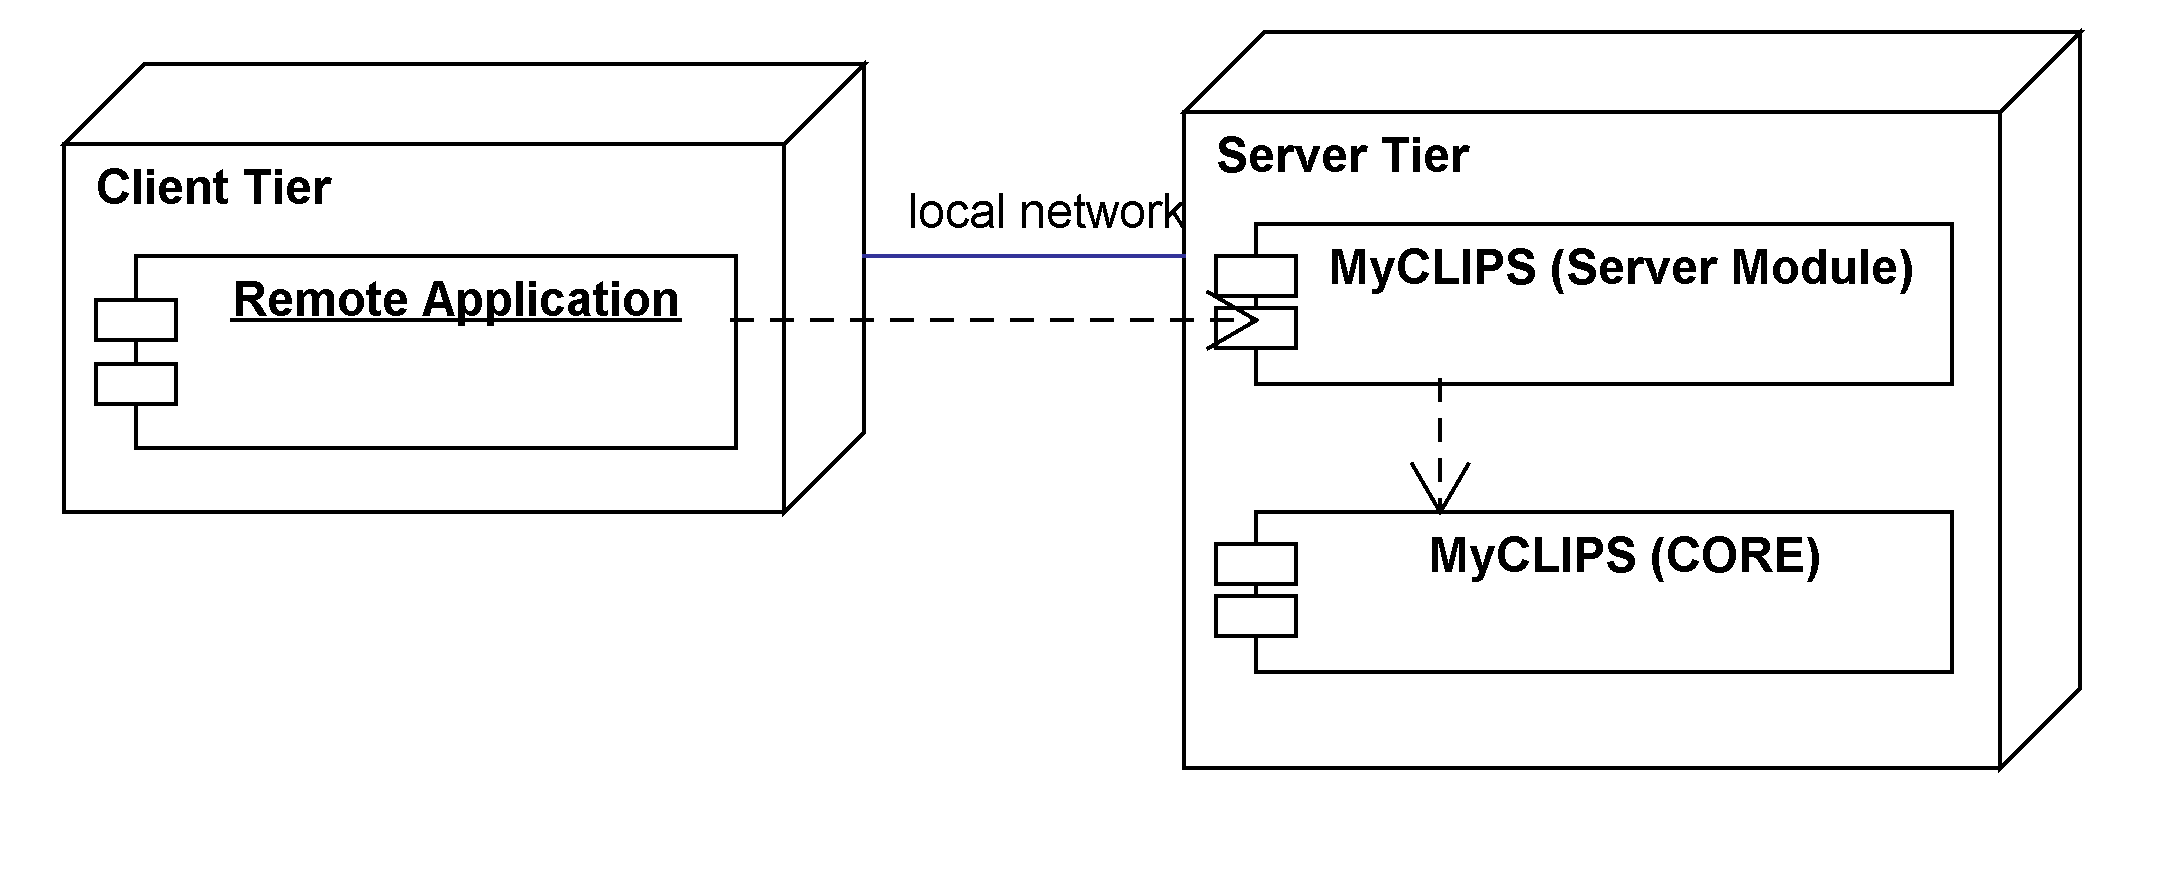
\includegraphics[width=0.8\textwidth]{Immagini/Capitolo3/Deployment/Client-Server.png}
\caption[Vista generale dell'architettura di sistema]{Vista generale dell'architettura di sistema: i servizi offerti dal modulo principale vengono distribuiti ad una serie di applicazioni remote attraverso l'utilizzo del componente Server}\label{fig:architettura-client-server}
\end{figure}

Il sistema è composto da due componenti principali distinte. Una prima, il \emph{core} del sistema MyCLIPS, realizza i servizi previsti dall'environment in una serie di API. Una seconda, il \emph{modulo server}, si pone come tramite fra i servizi offerti dalla prima componente e un gruppo di client, distribuendo le caratteristiche attraverso un modello d'architettura \emph{Client-Server}~(\figurename~\ref{fig:architettura-client-server}).

\begin{figure}[h]
\centering
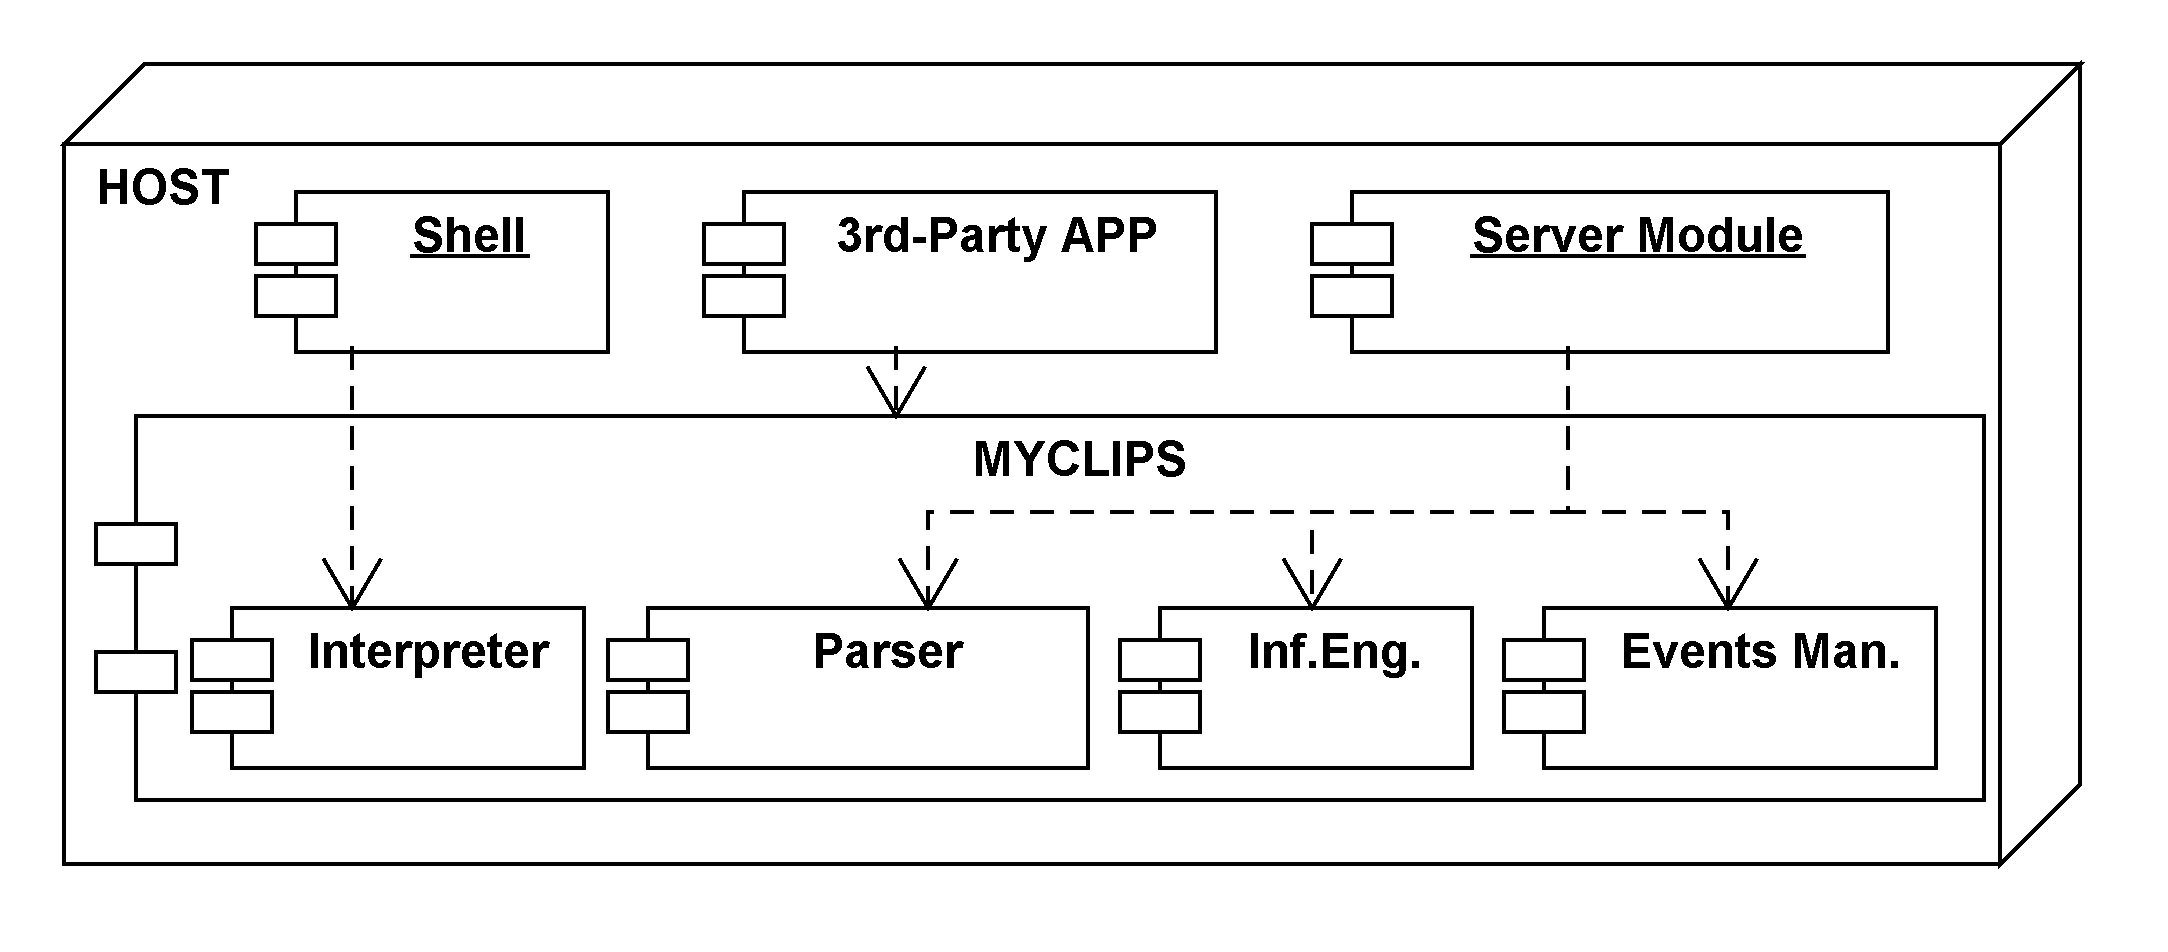
\includegraphics[width=0.9\textwidth]{Immagini/Capitolo3/Deployment/Shell-3rdPartyApp.png}
\caption[Vista generale dell'architettura locale di sistema]{Vista generale dell'architettura locale di sistema: i componenti del \emph{core} vengono utilizzati da componenti esterne (\emph{shell}, \emph{modulo server} o applicazioni generiche)}\label{fig:architettura-3rdparty}
\end{figure}

Il \emph{modulo server} è sia un elemento di sistema che un esempio d'istanza di applicazione generica che utilizza i servizi offerti dal \emph{core}. Un altro esempio è quello del componente \emph{shell}: un elemento distinto che utilizza le interfacce del \emph{core} per realizzare un terminale testuale con il quale utilizzare l'\emph{environment}~(\figurename~\ref{fig:architettura-3rdparty}).


\subsection{Core}

La componente principale è quella rappresentata dal \emph{core} di MyCLIPS: racchiude tutti i \emph{package} necessari alla realizzazione dei servizi principali del sistema~(\figurename~\ref{fig:packages-myclips}).

\begin{figure}[h]
\centering
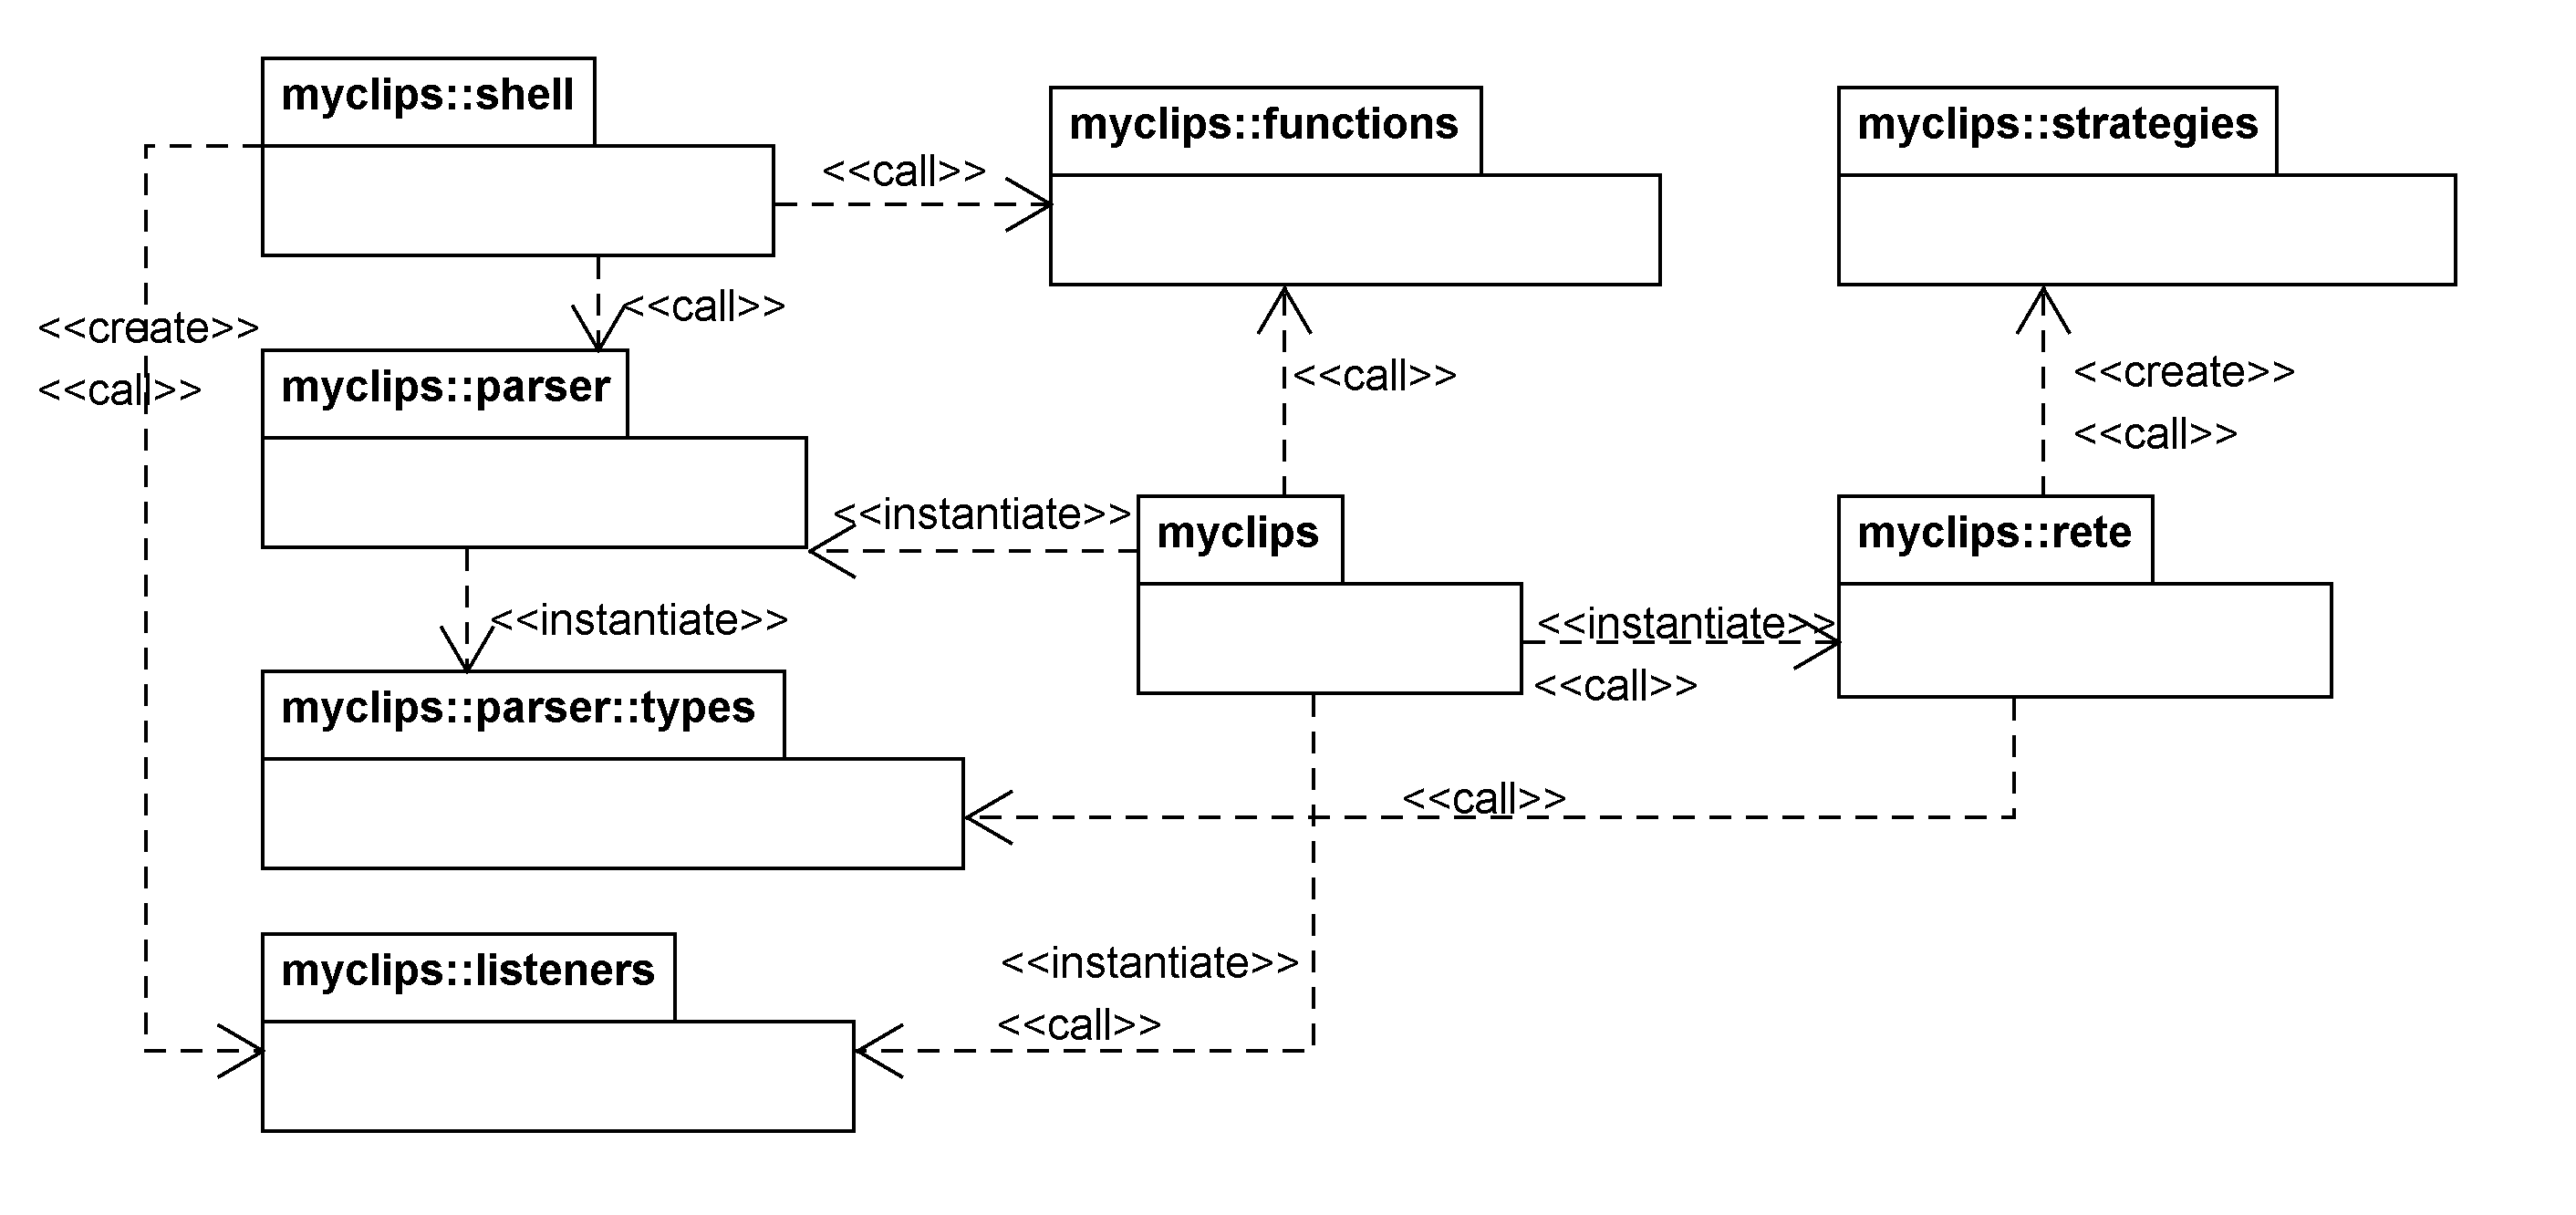
\includegraphics[width=1\textwidth]{Immagini/Capitolo3/Packages/Core.png}
\caption{Package \emph{myclips}: vista dei \emph{package} che compongono il \emph{core}}\label{fig:packages-myclips}
\end{figure}

%Lo scopo dei singoli \emph{package}, con riferimento alle funzionalità che realizzano, è dettagliato nel proseguo dei paragrafi.

\subsubsection{Modulo Parser}

\begin{figure}[h]
\centering
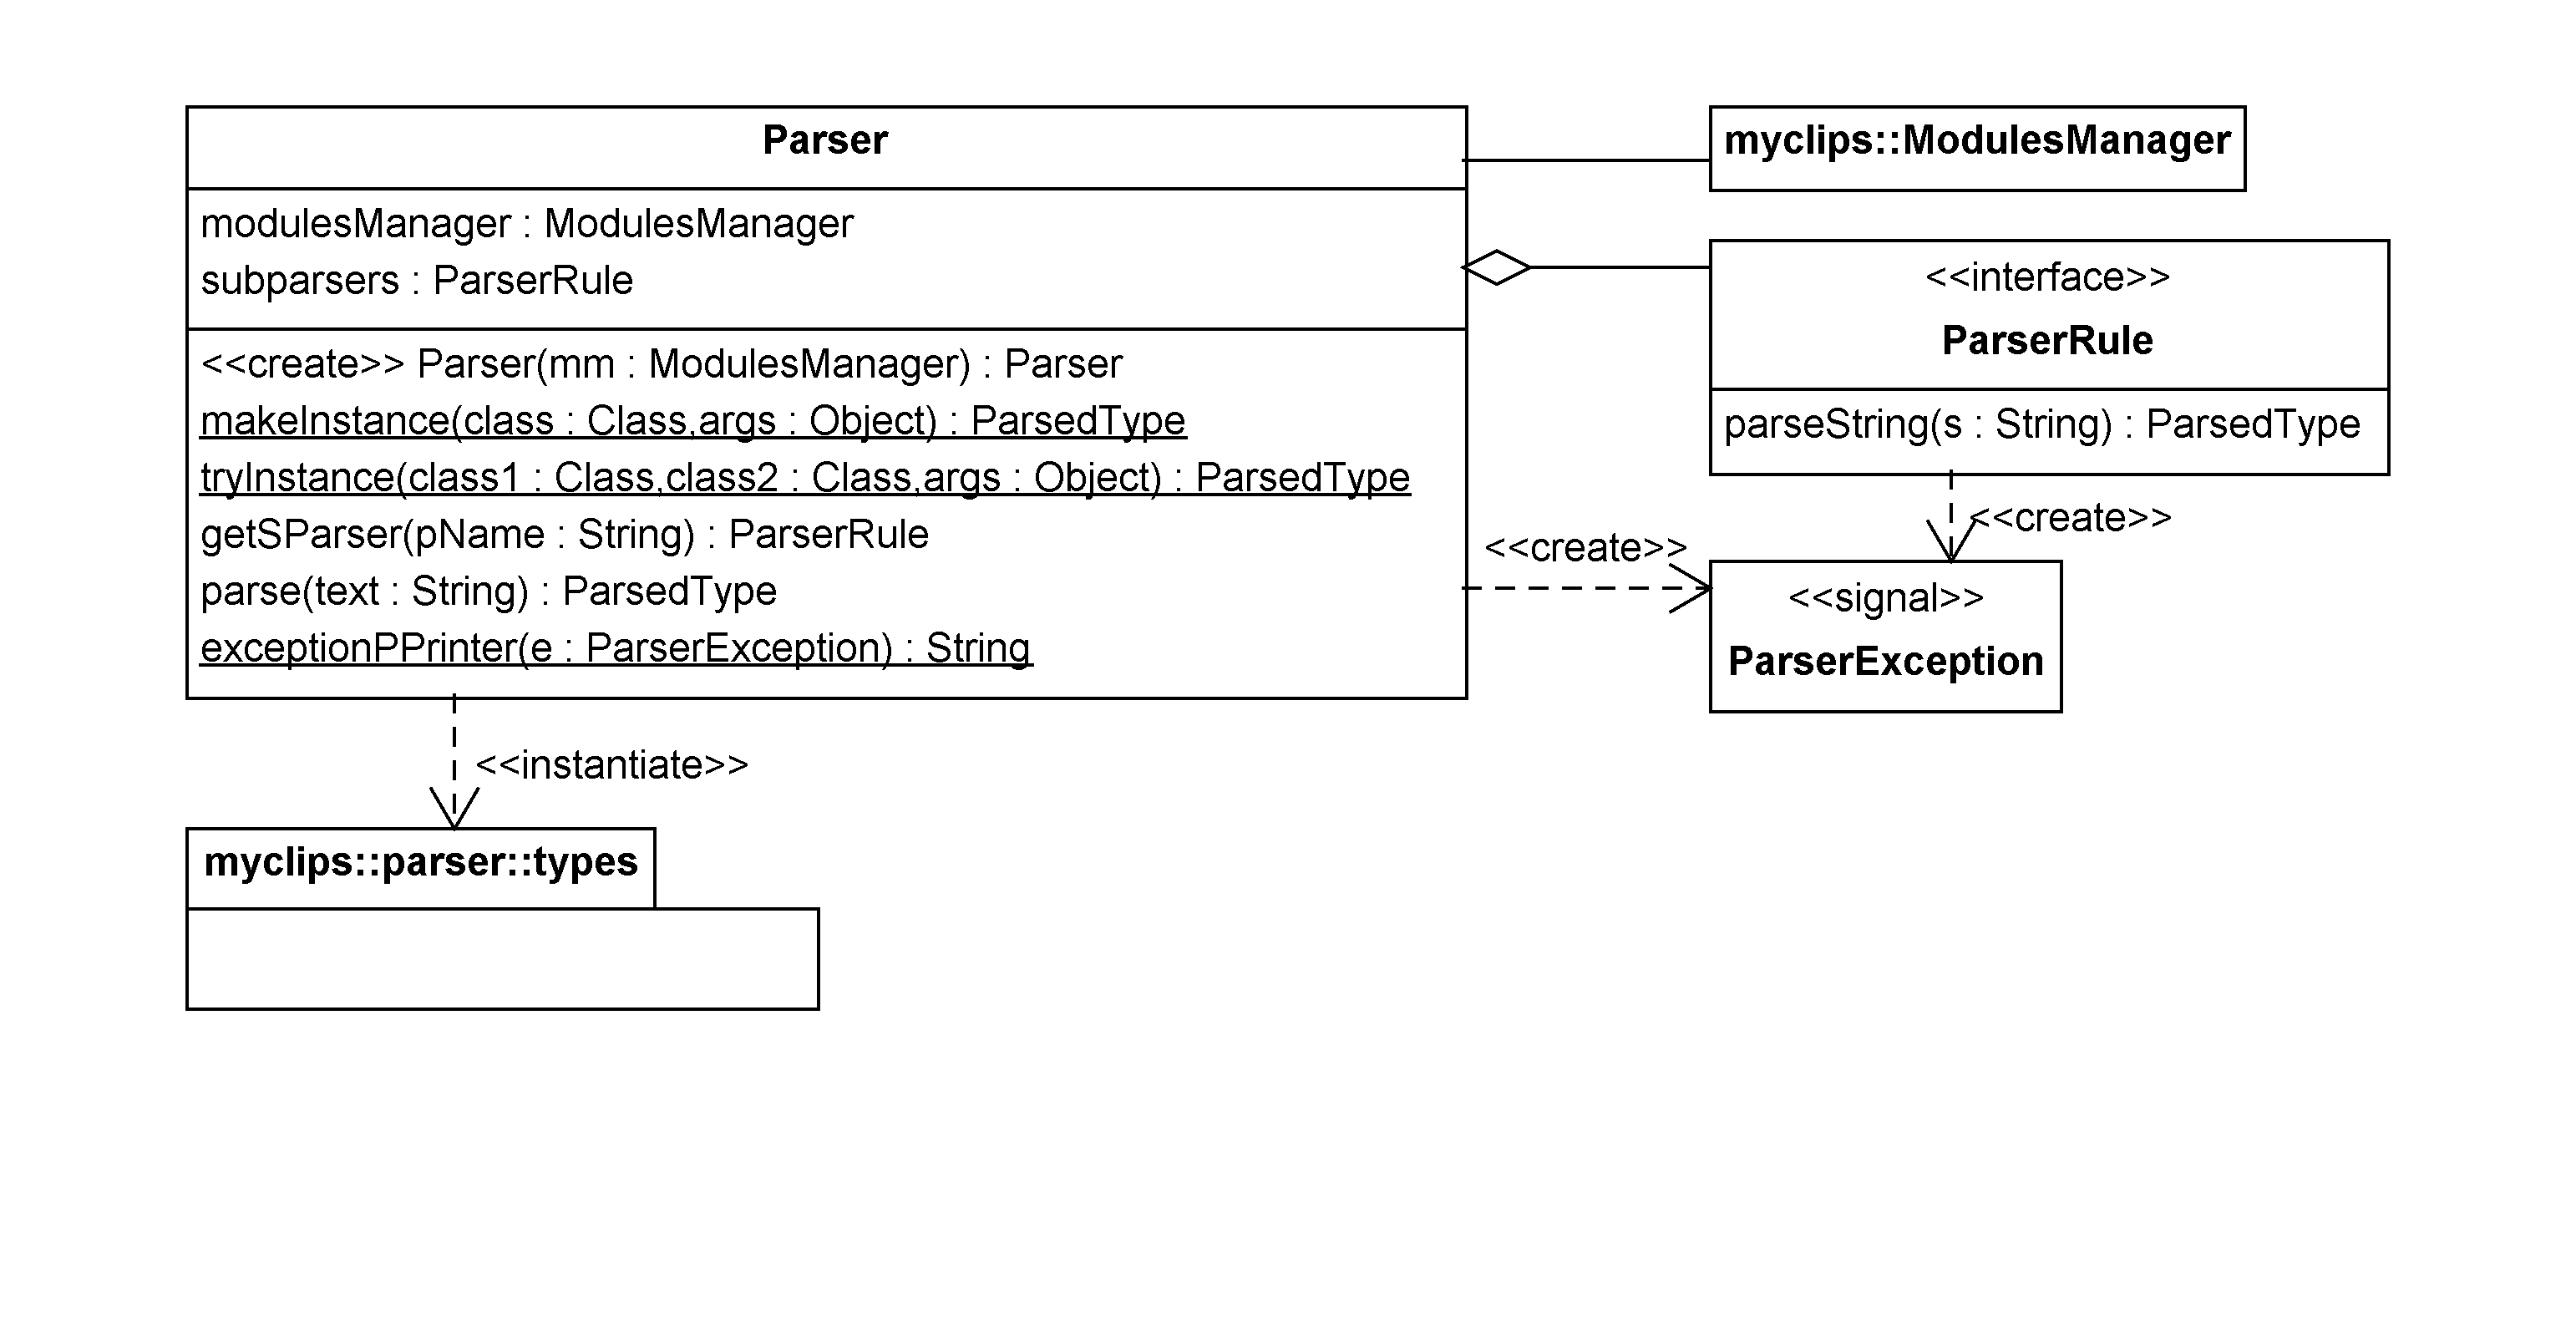
\includegraphics[width=1\textwidth]{Immagini/Capitolo3/Classi/myclips_parser_Parser.png}
\caption{Package \emph{myclips.parser}: vista delle classi relative al \emph{Parser}}\label{fig:class-myclips-parser-Parser}
\end{figure}

Il \emph{package} \emph{Parser} comprende l'insieme di classi e interfacce che realizzano la funzionalità di analisi e conversione del linguaggio di specifica in istanze utilizzabili dal motore inferenziale per il compimento delle proprie attività.

L'elemento principale del \emph{package} è la classe \emph{Parser}~(\figurename~\ref{fig:class-myclips-parser-Parser}), che organizza le regole di conversione (rappresentate dall'interfaccia \emph{ParserRule}) ed effettua le operazioni di conversione del testo in istanze. Le classi utilizzate per la rappresentazione dei costrutti convertiti sono organizzate all'interno del \emph{sub-package} \emph{myclips.parser.types}.

Il \emph{sub-package} contiene l'insieme di classi relative alla rappresentazione dei tipi atomici di base e dei costrutti compositi.

\begin{figure}[h]
\centering
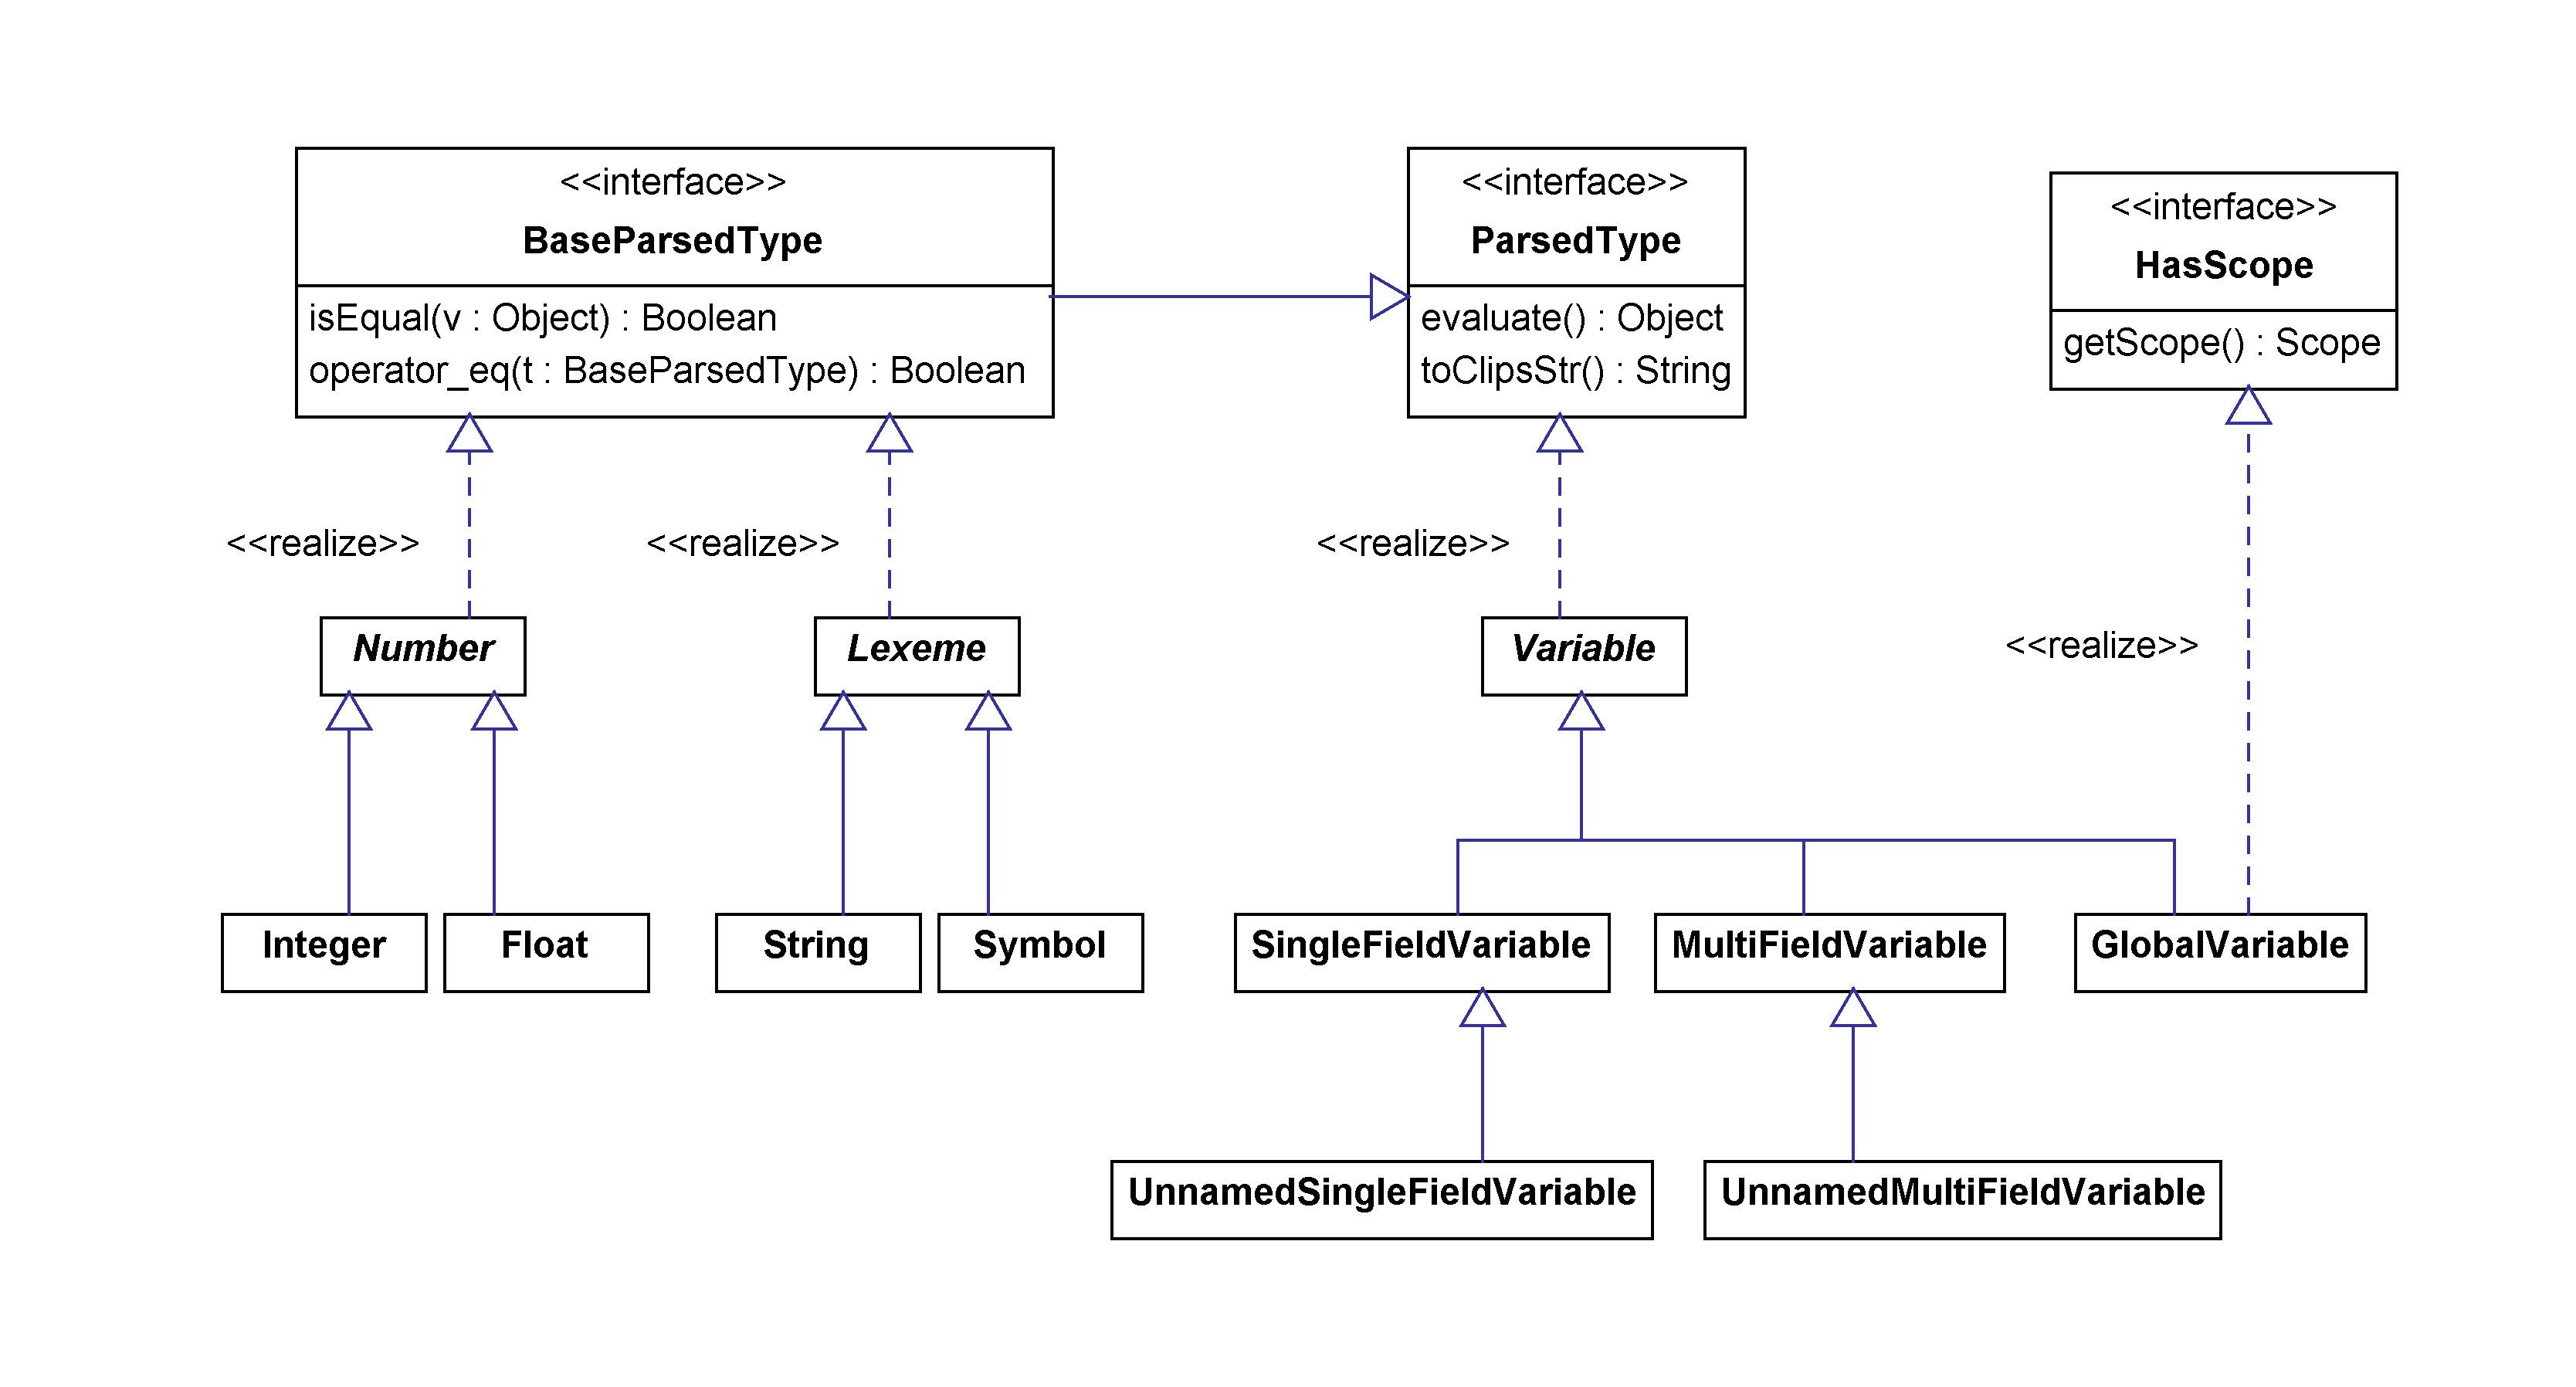
\includegraphics[width=0.8\textwidth]{Immagini/Capitolo3/Classi/myclips_parser_types_Atoms.png}
\caption{Package \emph{myclips.parser.types}: vista di classi e interfacce per gli elementi atomici}\label{fig:class-myclips-parser-types-Atoms}
\end{figure}

La gerarchia di tipi atomici supportata dal sistema segue le specifiche relative ai tipi proposti da CLIPS. Fanno parte di questa classificazione \emph{Lexeme}, specializzato da \emph{Symbol} e \emph{String}, e \emph{Number}, specializzato da \emph{Integer} e \emph{Float}. A questi tipi si uniscono quelli per la rappresentazioni delle variabili~(\figurename~\ref{fig:class-myclips-parser-types-Atoms}).

\begin{figure}[h]
\centering
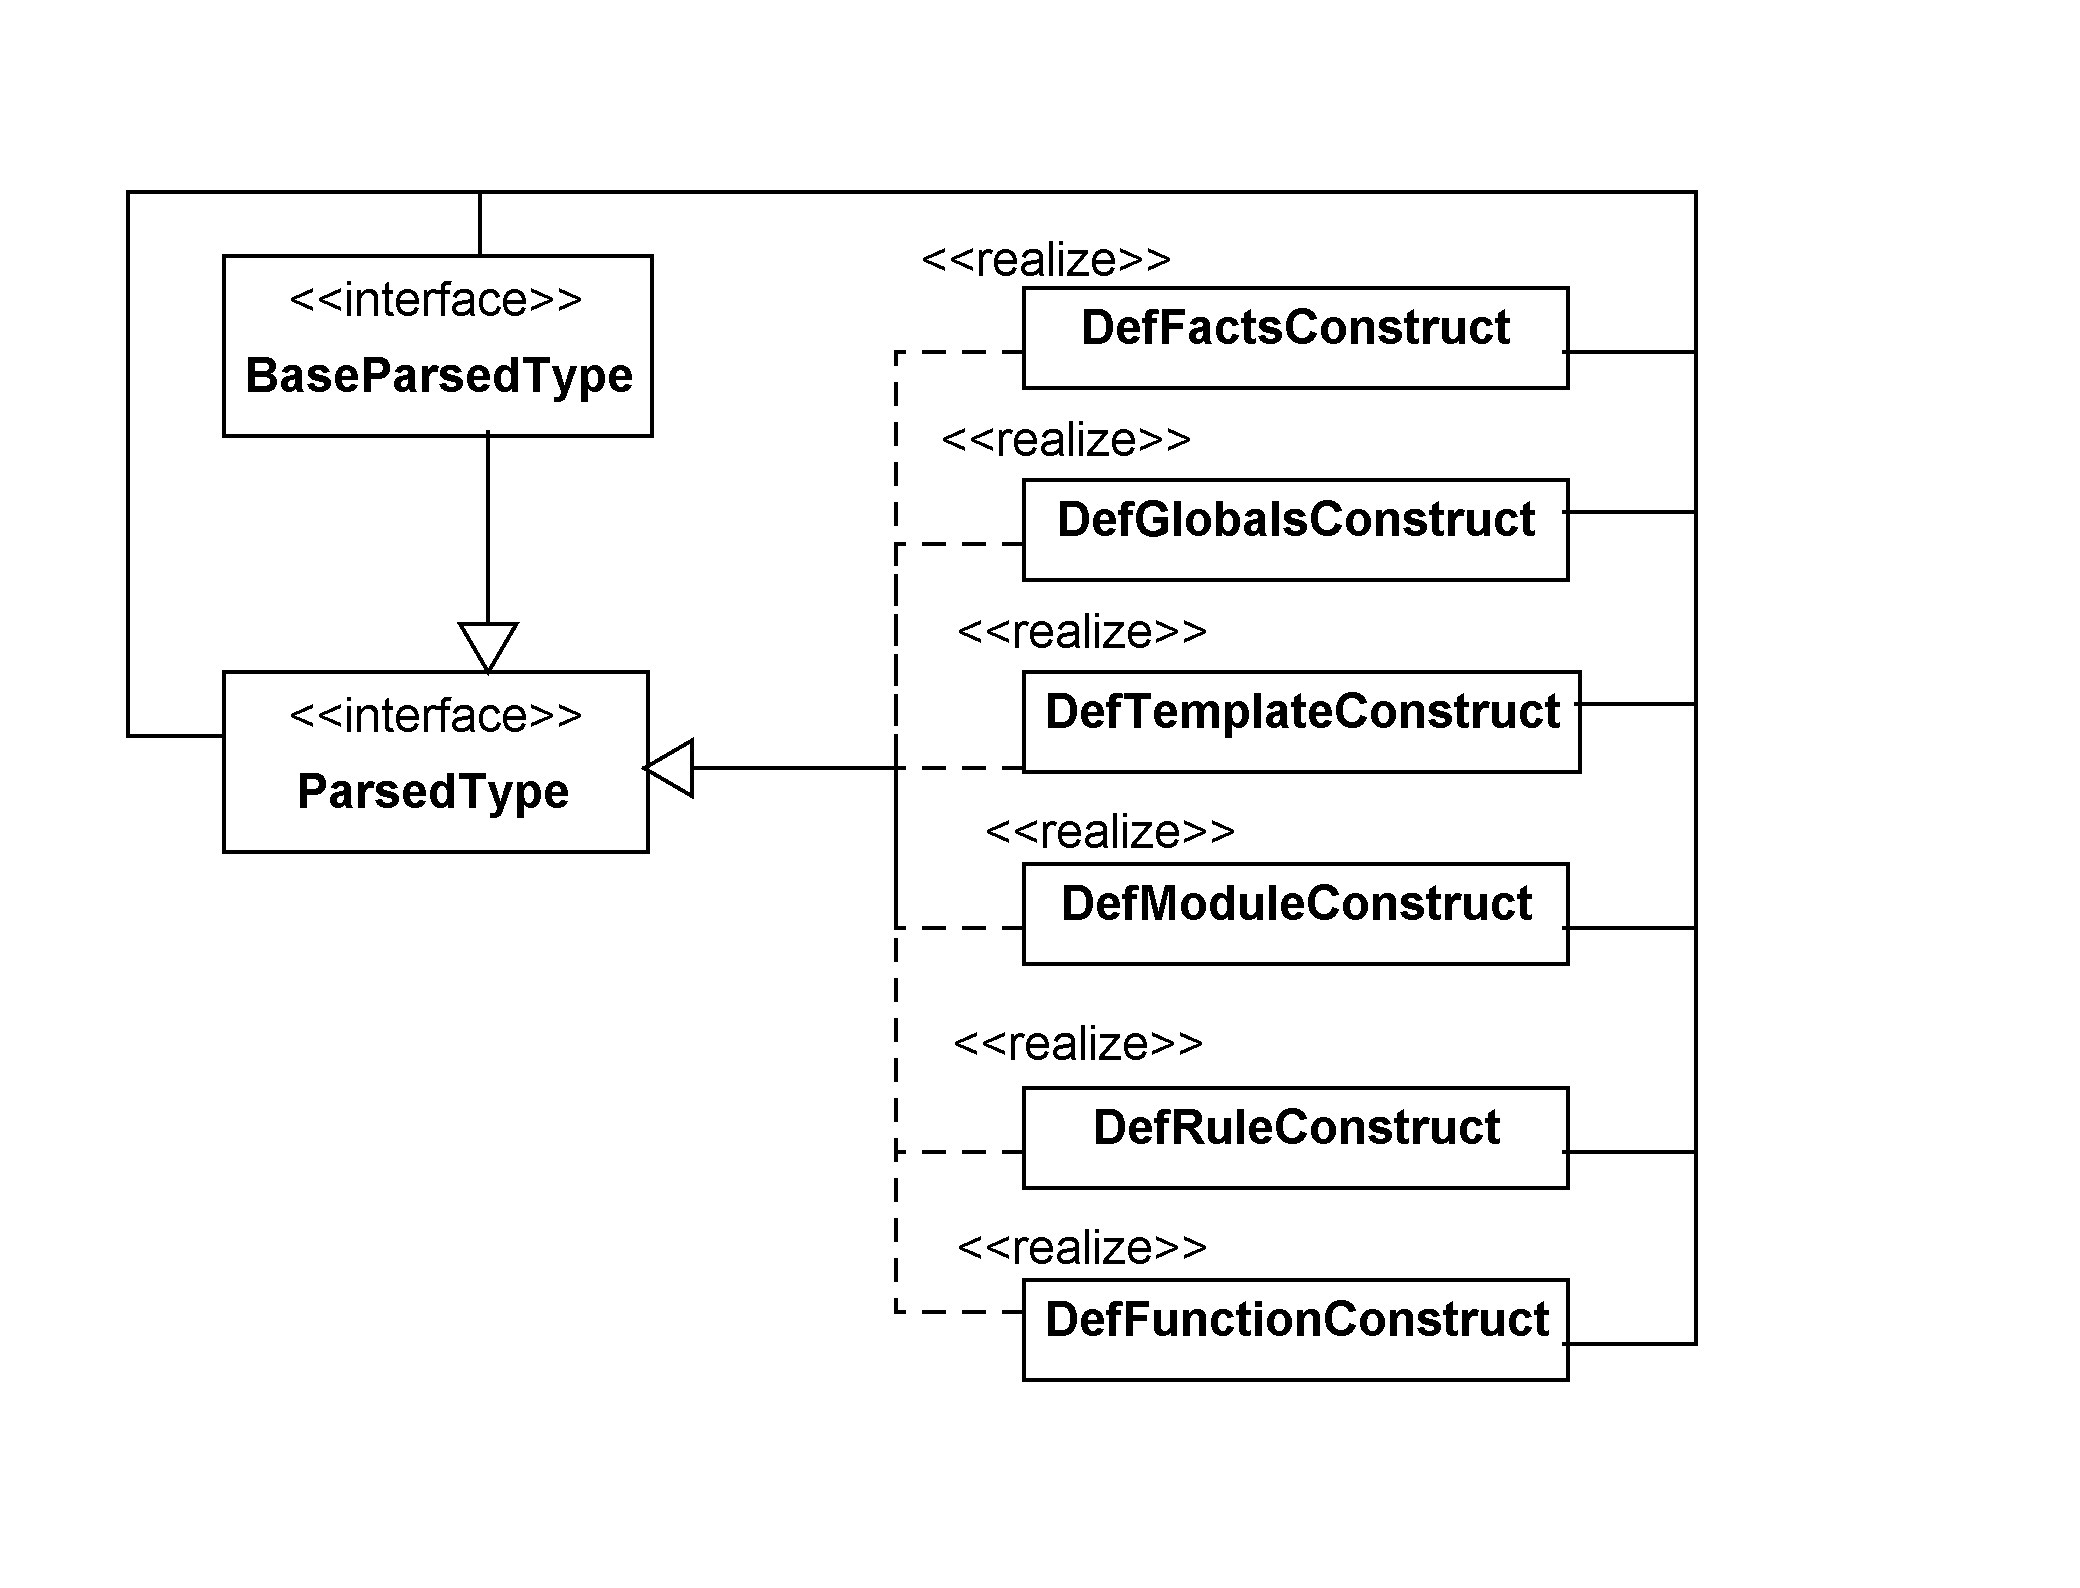
\includegraphics[width=0.8\textwidth]{Immagini/Capitolo3/Classi/myclips_parser_types_Constructs.png}
\caption{Package \emph{myclips.parser.types}: vista di classi e interfacce per i costrutti principali}\label{fig:class-myclips-parser-types-Constructs}
\end{figure}

La composizione dei tipi di base realizza un insieme di costrutti complessi principali. Le classi mostrate in \figurename~\ref{fig:class-myclips-parser-types-Constructs} sono le rappresentazioni corrispondenti ai formalismi \emph{defrule}, \emph{defglobals}, \emph{deffunction}, \emph{deftemplate} e \emph{defmodule}, utilizzate dal linguaggio di specifica per la formalizzazione dei sistemi esperti.

\begin{figure}[h]
\centering
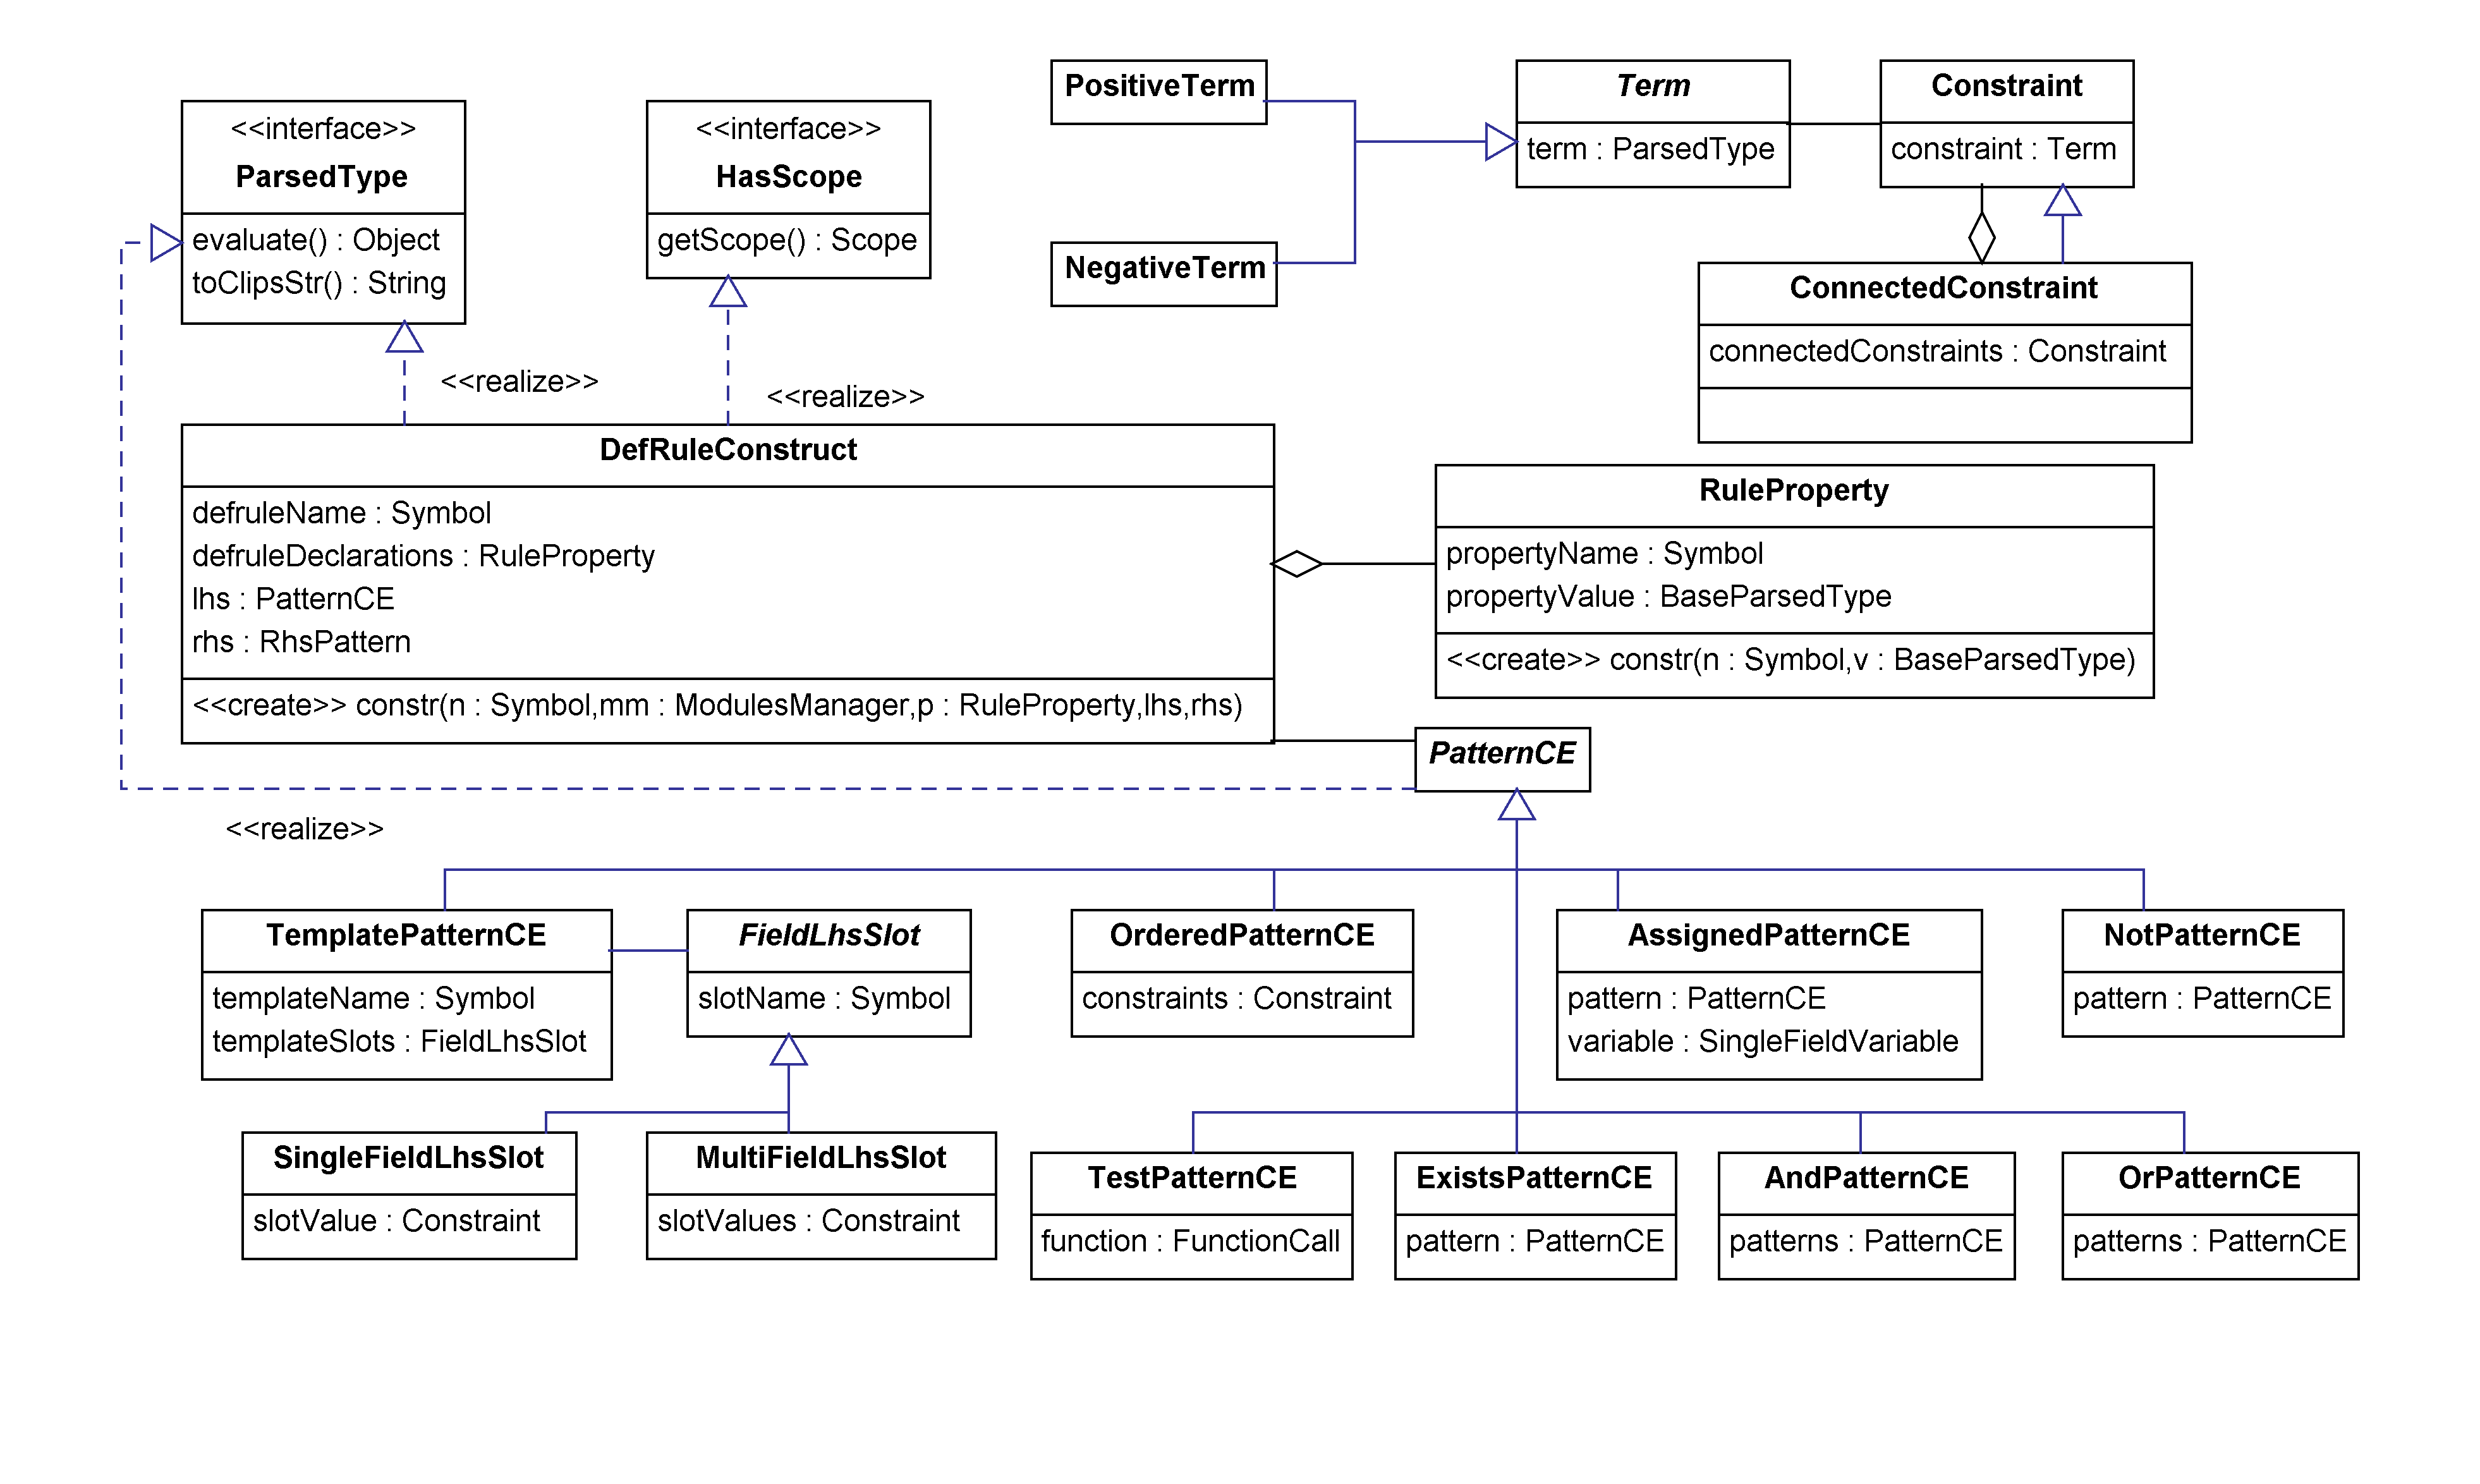
\includegraphics[width=1\textwidth]{Immagini/Capitolo3/Classi/myclips_parser_types_DefRule.png}
\caption{Package \emph{myclips.parser.types}: vista delle classi e interfacce relative al costrutto \emph{defrule}}\label{fig:class-myclips-parser-types-DefRuleConstruct}
\end{figure}

%\begin{figure}[h]
%\centering
%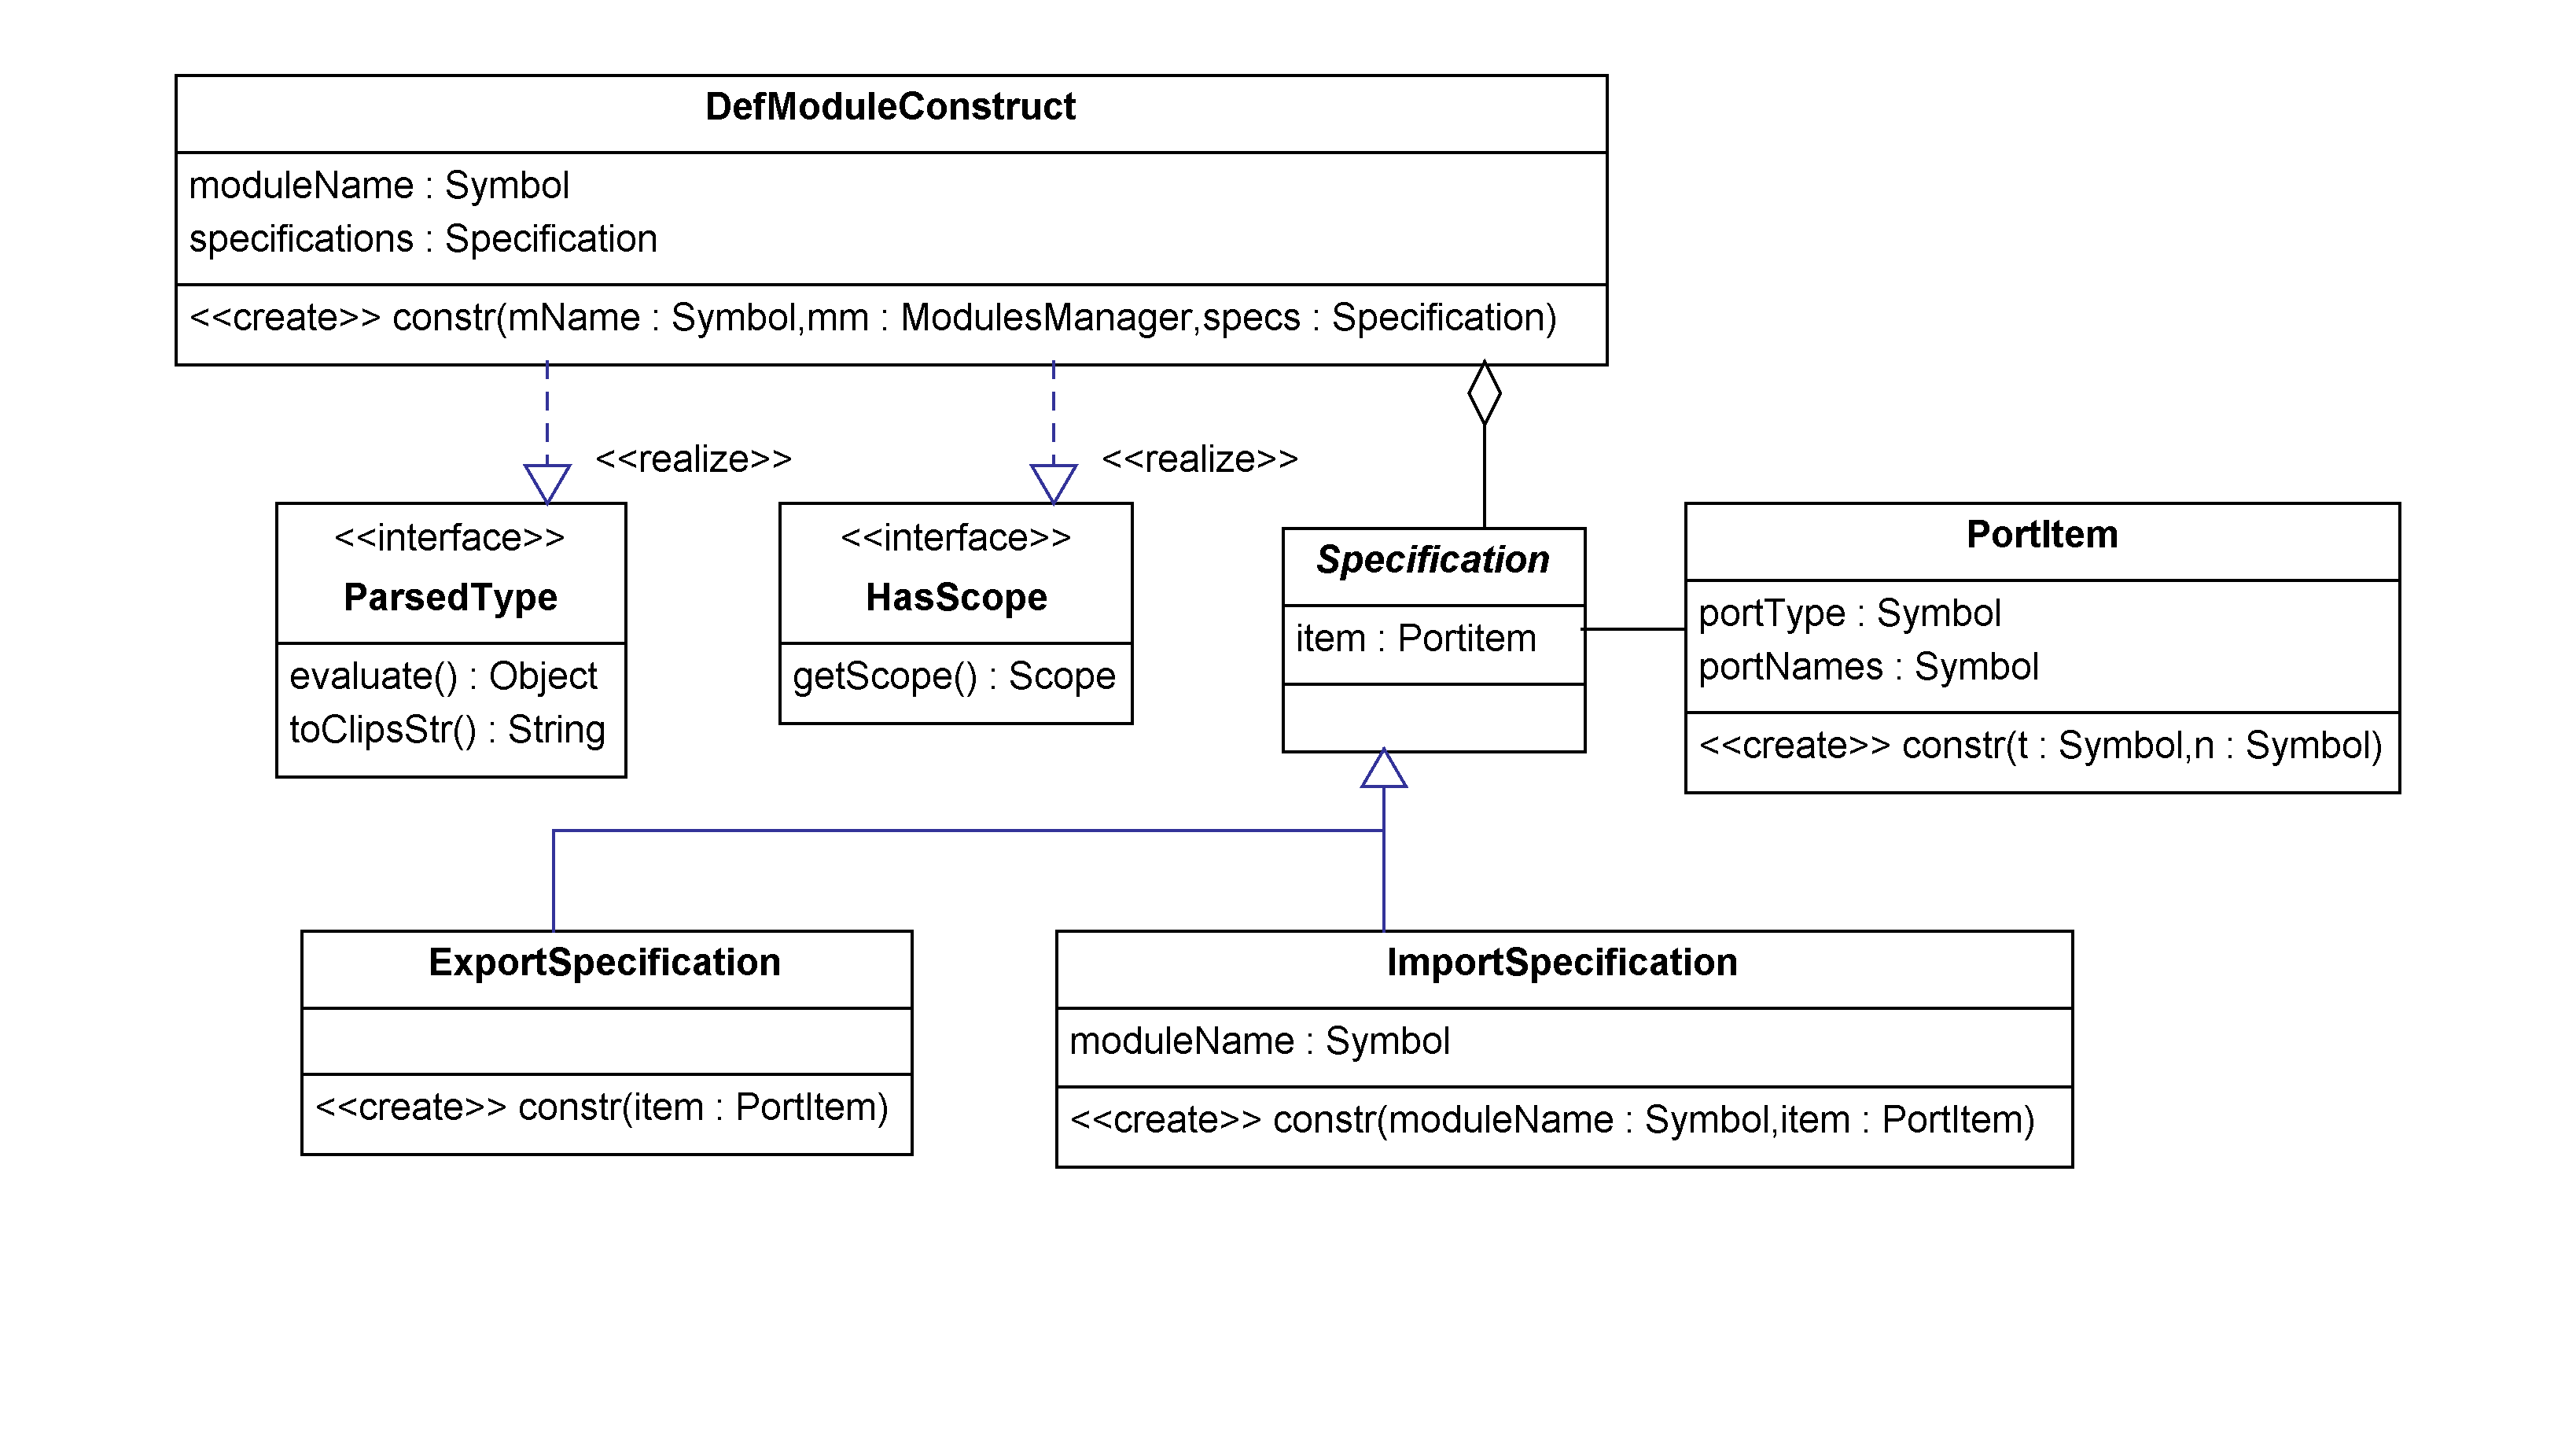
\includegraphics[width=0.9\textwidth]{Immagini/Capitolo3/Classi/myclips_parser_types_DefModule.png}
%\caption{Package \emph{myclips.parser.types}: vista delle classi e interfacce relative al costrutto \emph{defmodule}}\label{fig:class-myclips-parser-types-DefModuleConstruct}
%\end{figure}


%A titolo d'esempio di propongono le strutture delle classi \emph{DefRuleConstruct}~(\figurename~\ref{fig:class-myclips-parser-types-DefRuleConstruct}) e \emph{DefModuleConstruct}~(\figurename~\ref{fig:class-myclips-parser-types-DefModuleConstruct}), insieme ad i relativi sotto-costrutti utilizzati per la conversione e rappresentazione di pozioni di quest'ultimi.

A titolo d'esempio si propone la struttura della classe \emph{DefRuleConstruct}~(\figurename~\ref{fig:class-myclips-parser-types-DefRuleConstruct})  insieme ad i relativi sotto-costrutti utilizzati per la conversione e rappresentazione di pozioni di quest'ultima.


\subsubsection{Modulo Motore Inferenziale}

\begin{figure}[h]
\centering
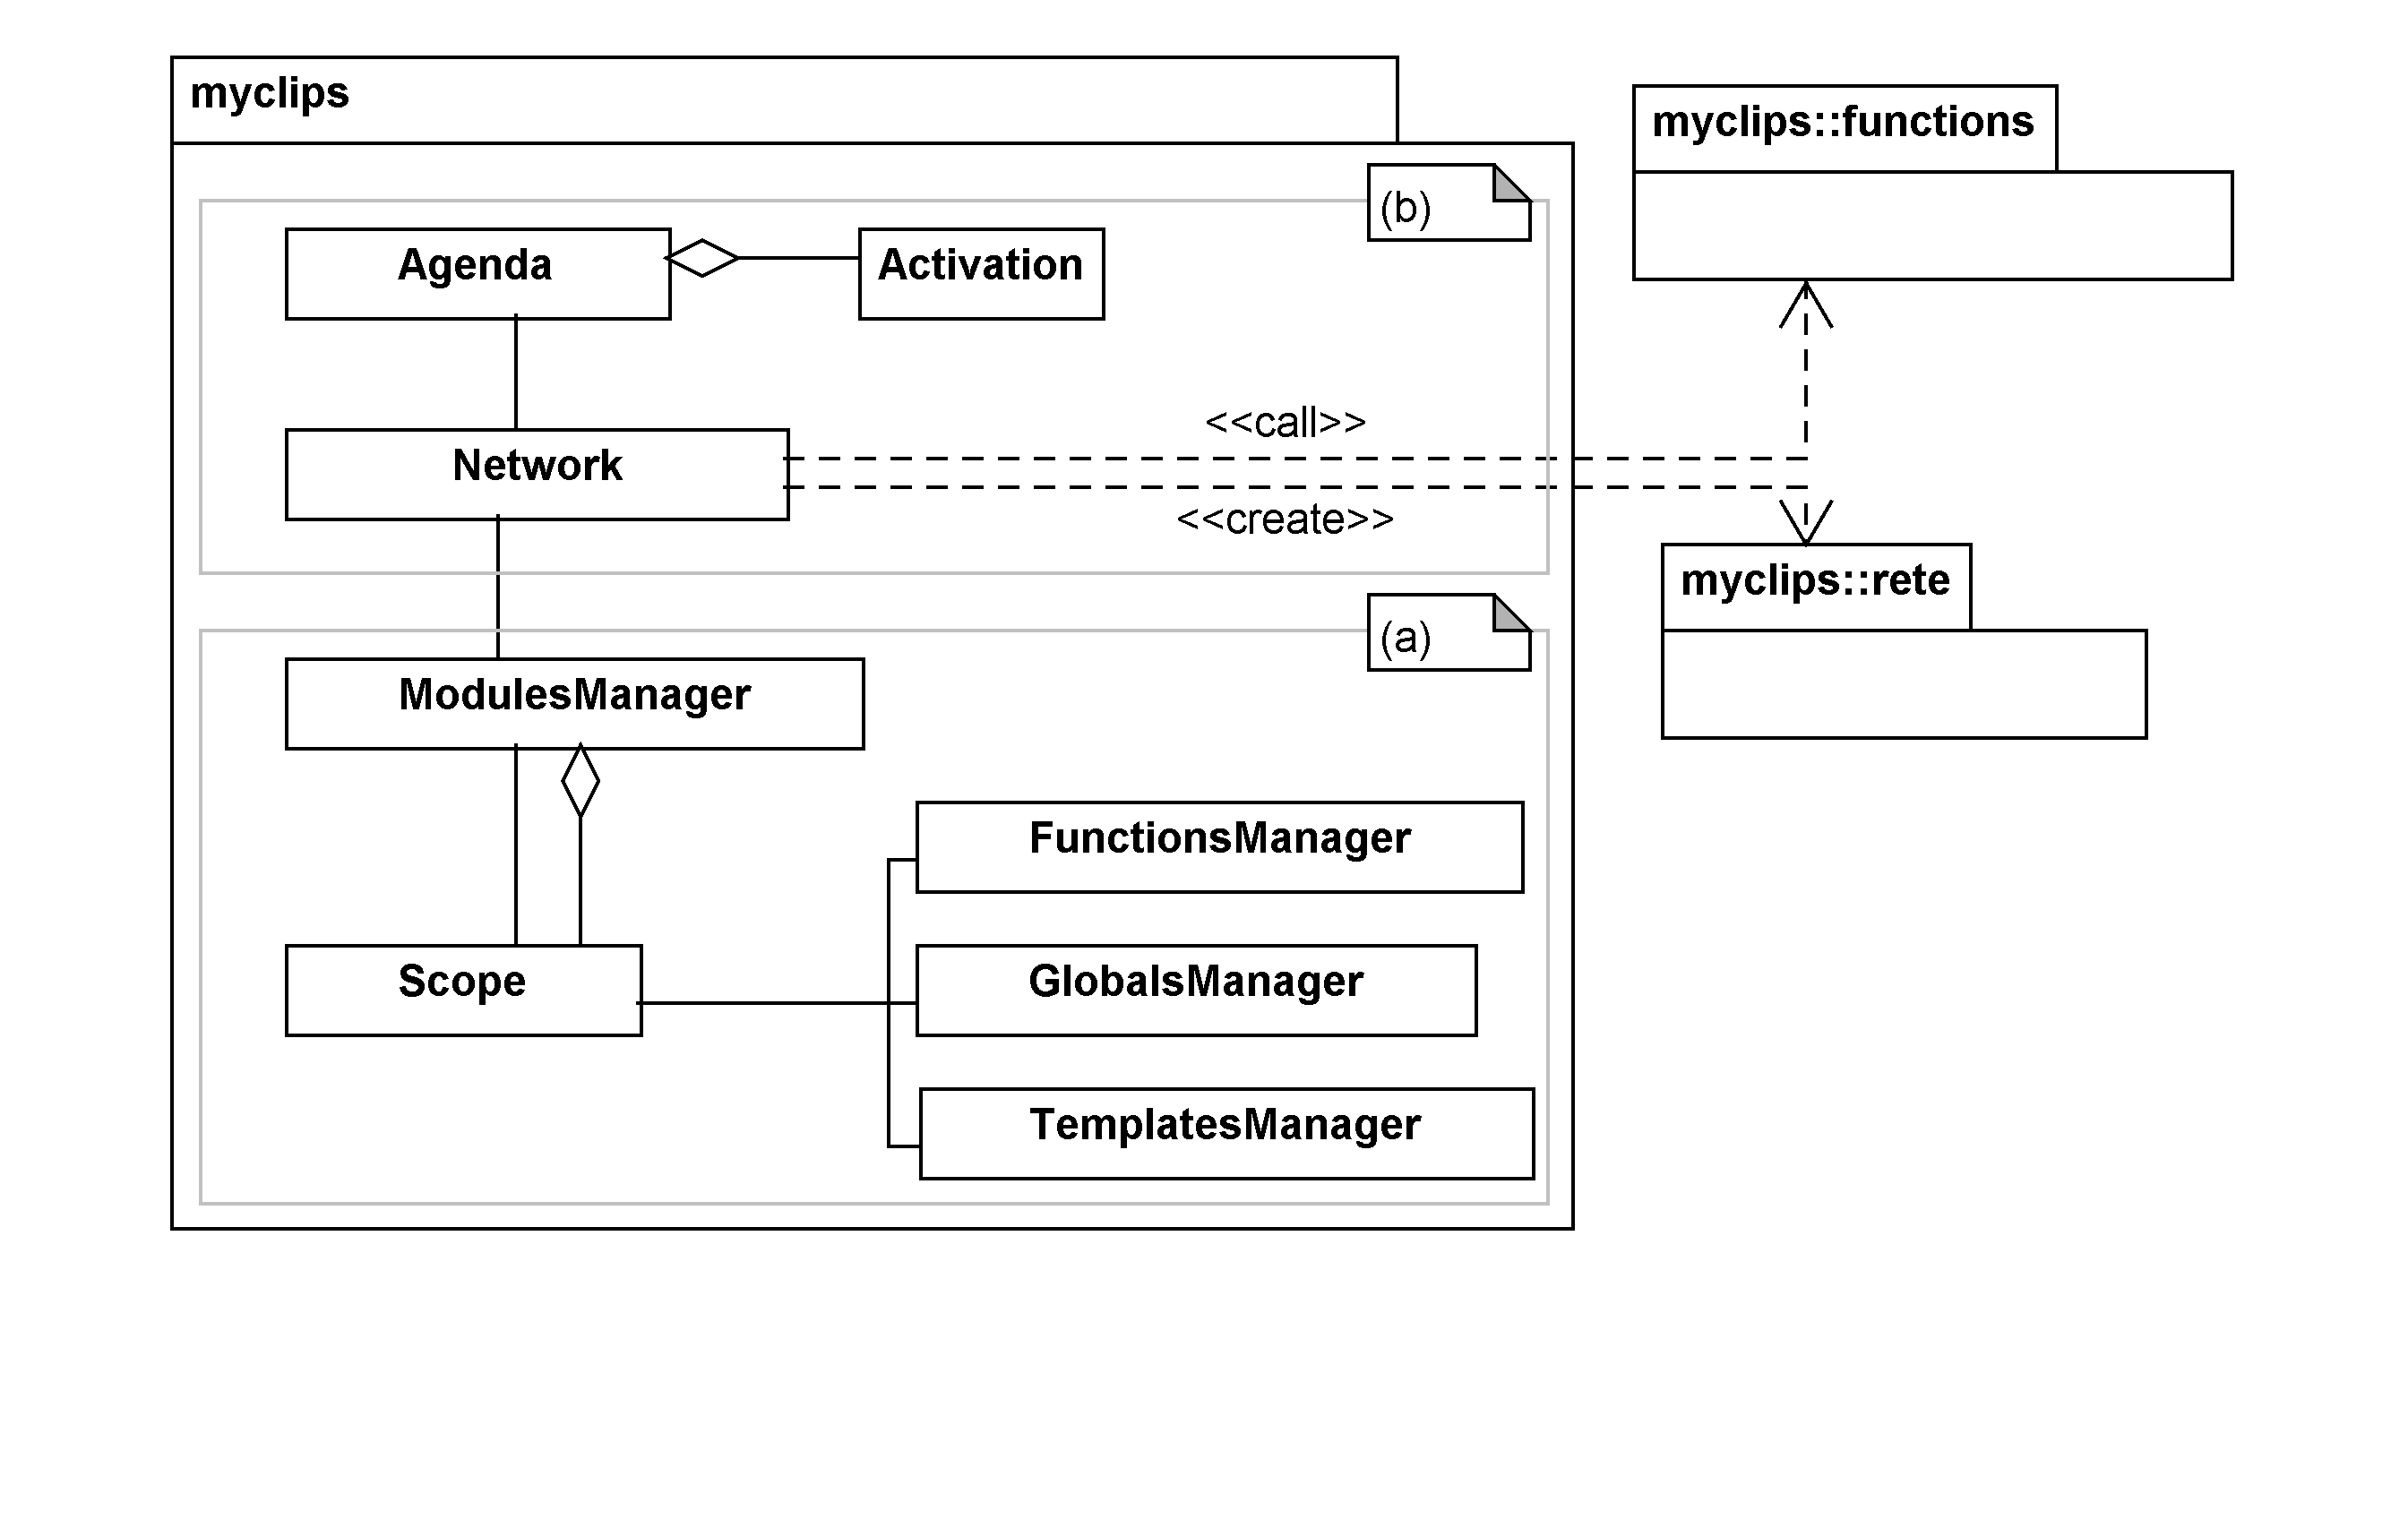
\includegraphics[width=1\textwidth]{Immagini/Capitolo3/Packages/IE.png}
\caption{Package \emph{myclips}: vista degli elementi che collaborano per la realizzazione dei servizi dell'\emph{IE}}\label{fig:packages-ie}
\end{figure}

Il ruolo del modulo \emph{Motore Inferenziale} (IE) è quello di offrire i servizi principali relativi alla gestione delle definizioni, all'esecuzione del ciclo \emph{recognize-act} e alla gestione delle transizioni fra gli stati del sistema.

A livello logico, le classi che lo realizzano possono essere raggruppate in due sezioni: una prima adibita alla gestione delle definizioni del sistema esperto (\figurename~\ref{fig:packages-ie}a), una seconda alla interpretazione e esecuzione dei costrutti (\figurename~\ref{fig:packages-ie}b).

\begin{figure}[h]
\centering
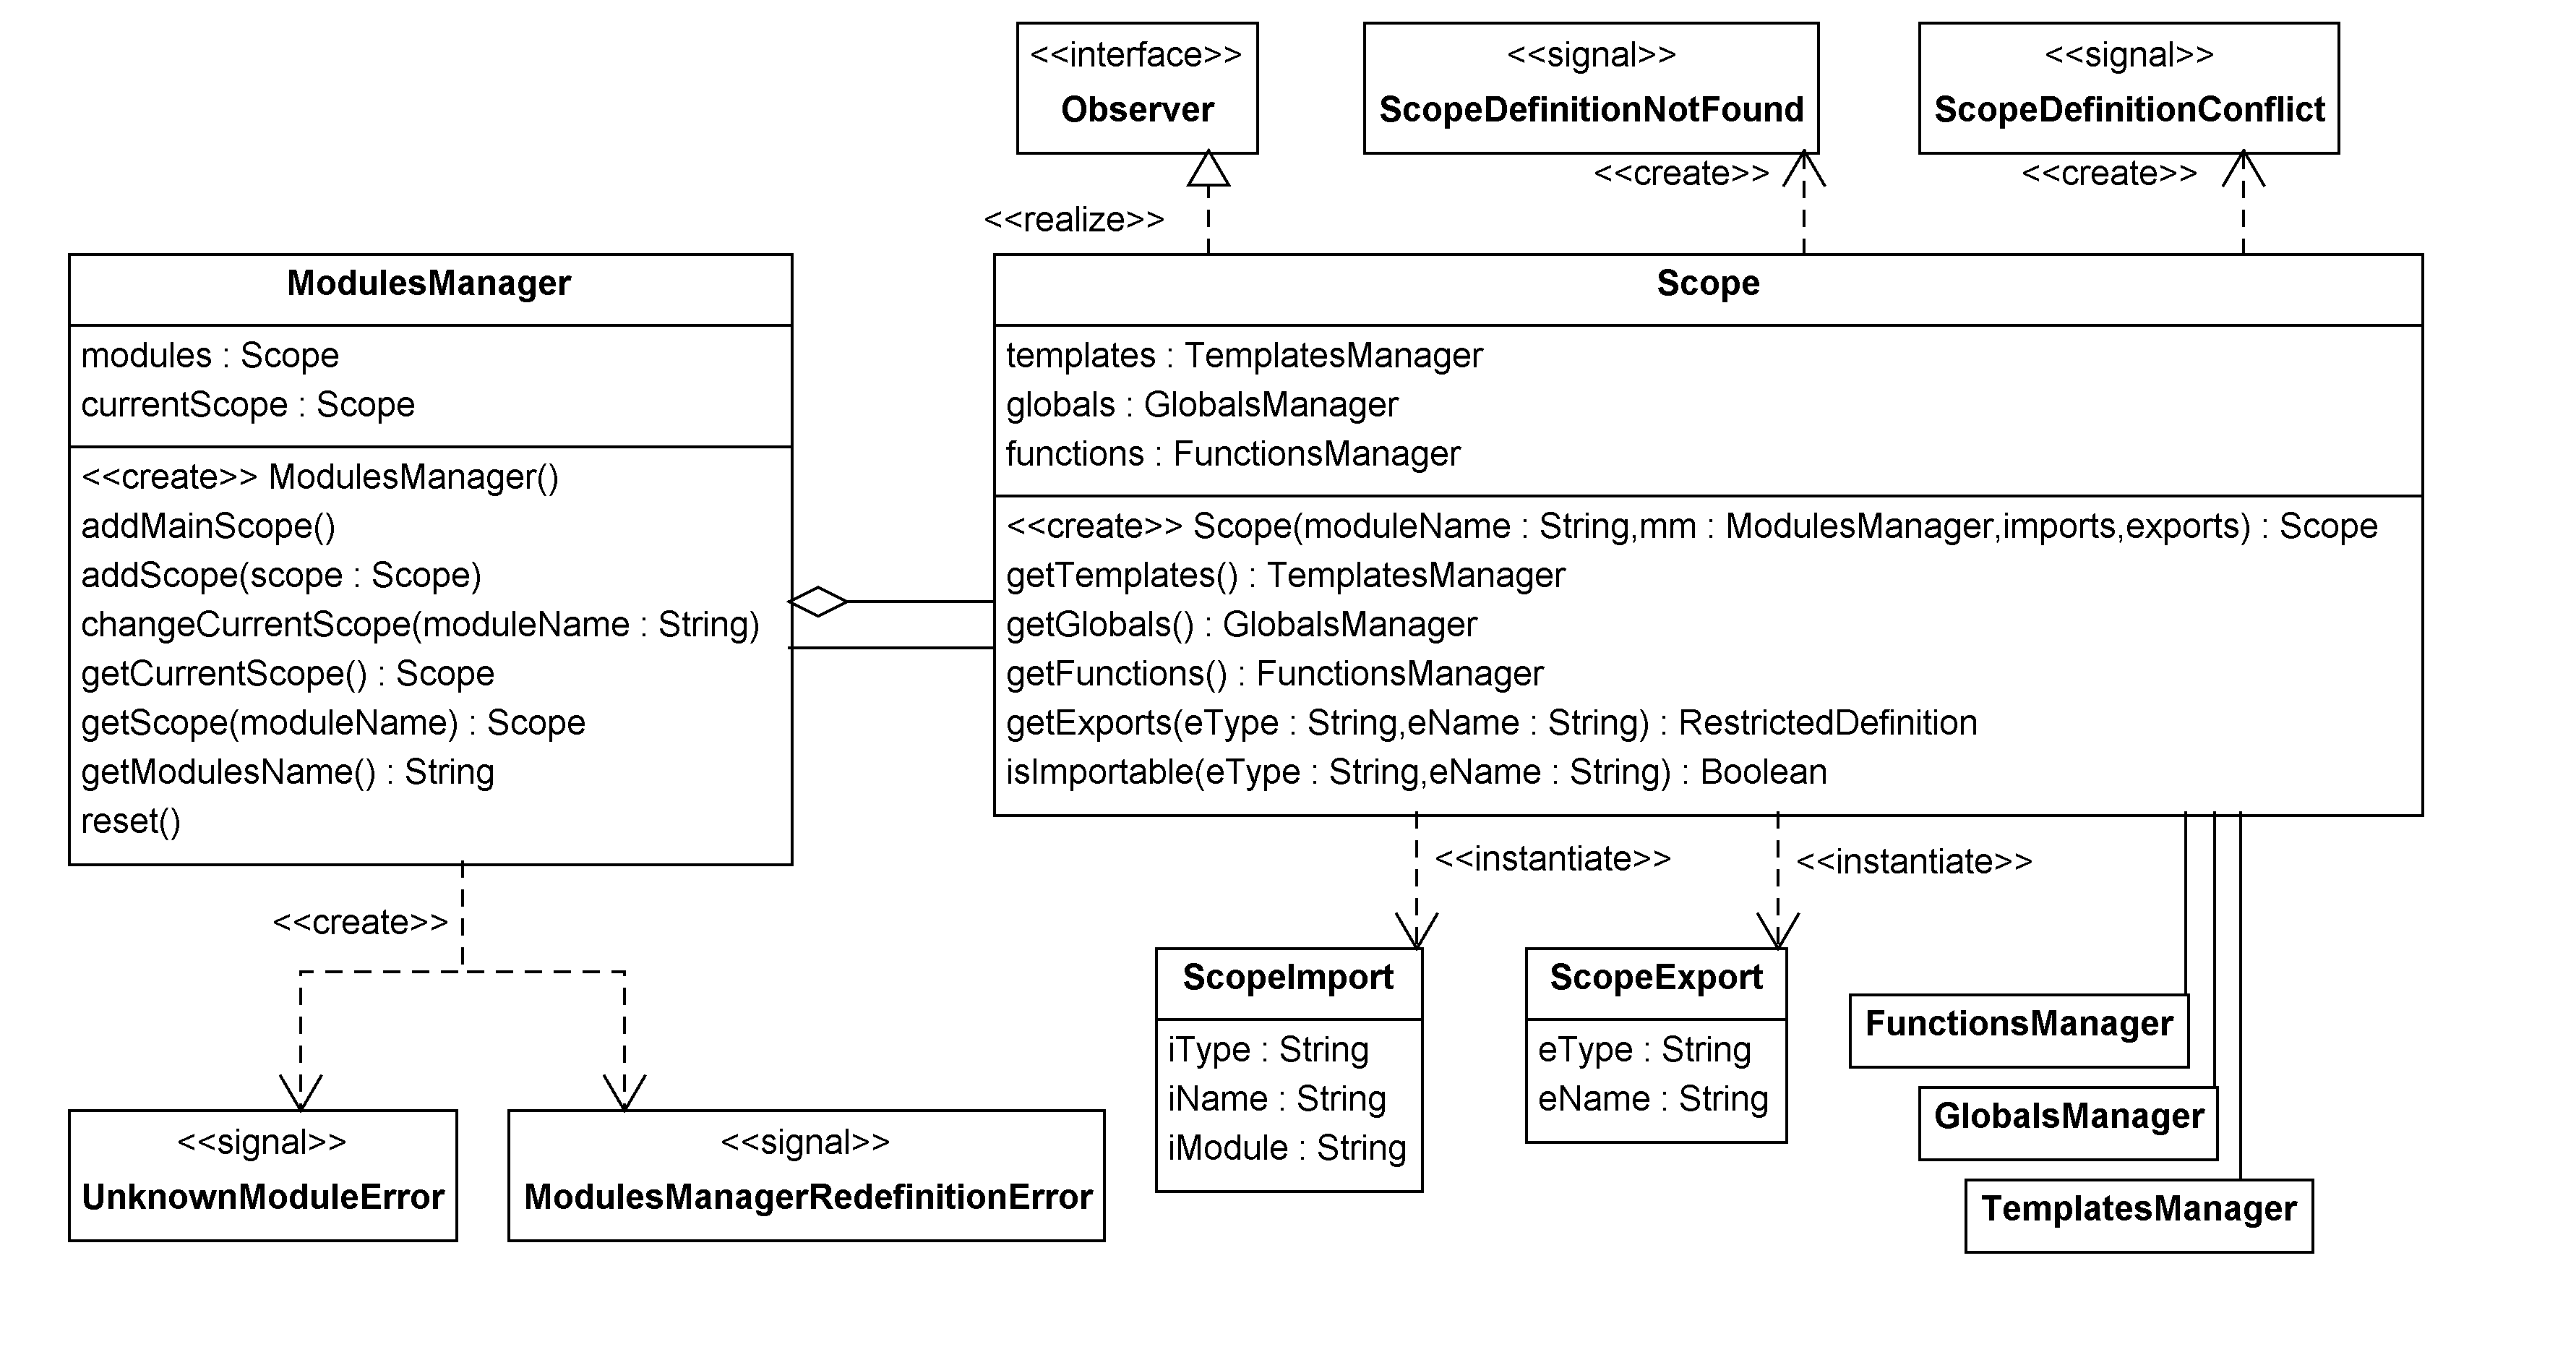
\includegraphics[width=1\textwidth]{Immagini/Capitolo3/Classi/myclips_Scope-ModulesManager.png}
\caption{Package \emph{myclips}: vista delle classi per la gestione dei moduli}\label{fig:class-myclips-scope-mm}
\end{figure}

\paragraph{Gestione delle definizioni}

La gestione dei moduli è affidata alla collaborazione fra le classi \emph{Scope} e \emph{ModulesManager}~(\figurename~\ref{fig:class-myclips-scope-mm}).
La classe \emph{ModulesManager} memorizza l'insieme dei moduli definiti in un sistema esperto e un attributo di stato (\emph{currentScope}) nel quale viene memorizzato il riferimento allo \emph{Scope} rappresentante il contesto corrente di esecuzione del sistema. Le definizioni o le azioni alle quali non è stato attribuito esplicitamente un modulo di appartenenza vengono automaticamente relazionate con il modulo corrente.

Le istanze di classe \emph{Scope} rappresentano singoli moduli definiti nel sistema. A differenza dell'entità \emph{modulo} intesa come collezione di costrutti e definizioni definiti nel \emph{modulo} stesso, quella di \emph{Scope} raggruppa l'insieme di definizioni disponibili in un preciso contesto d'uso relazionato ad un modulo. Ogni \emph{Scope} possiede i riferimenti ai manager dei tipi di costrutti definibili e gestisce il protocollo di \emph{import/export} delle definizioni~(\figurename~\ref{fig:sequence-def-import-export}).

\begin{figure}
\centering
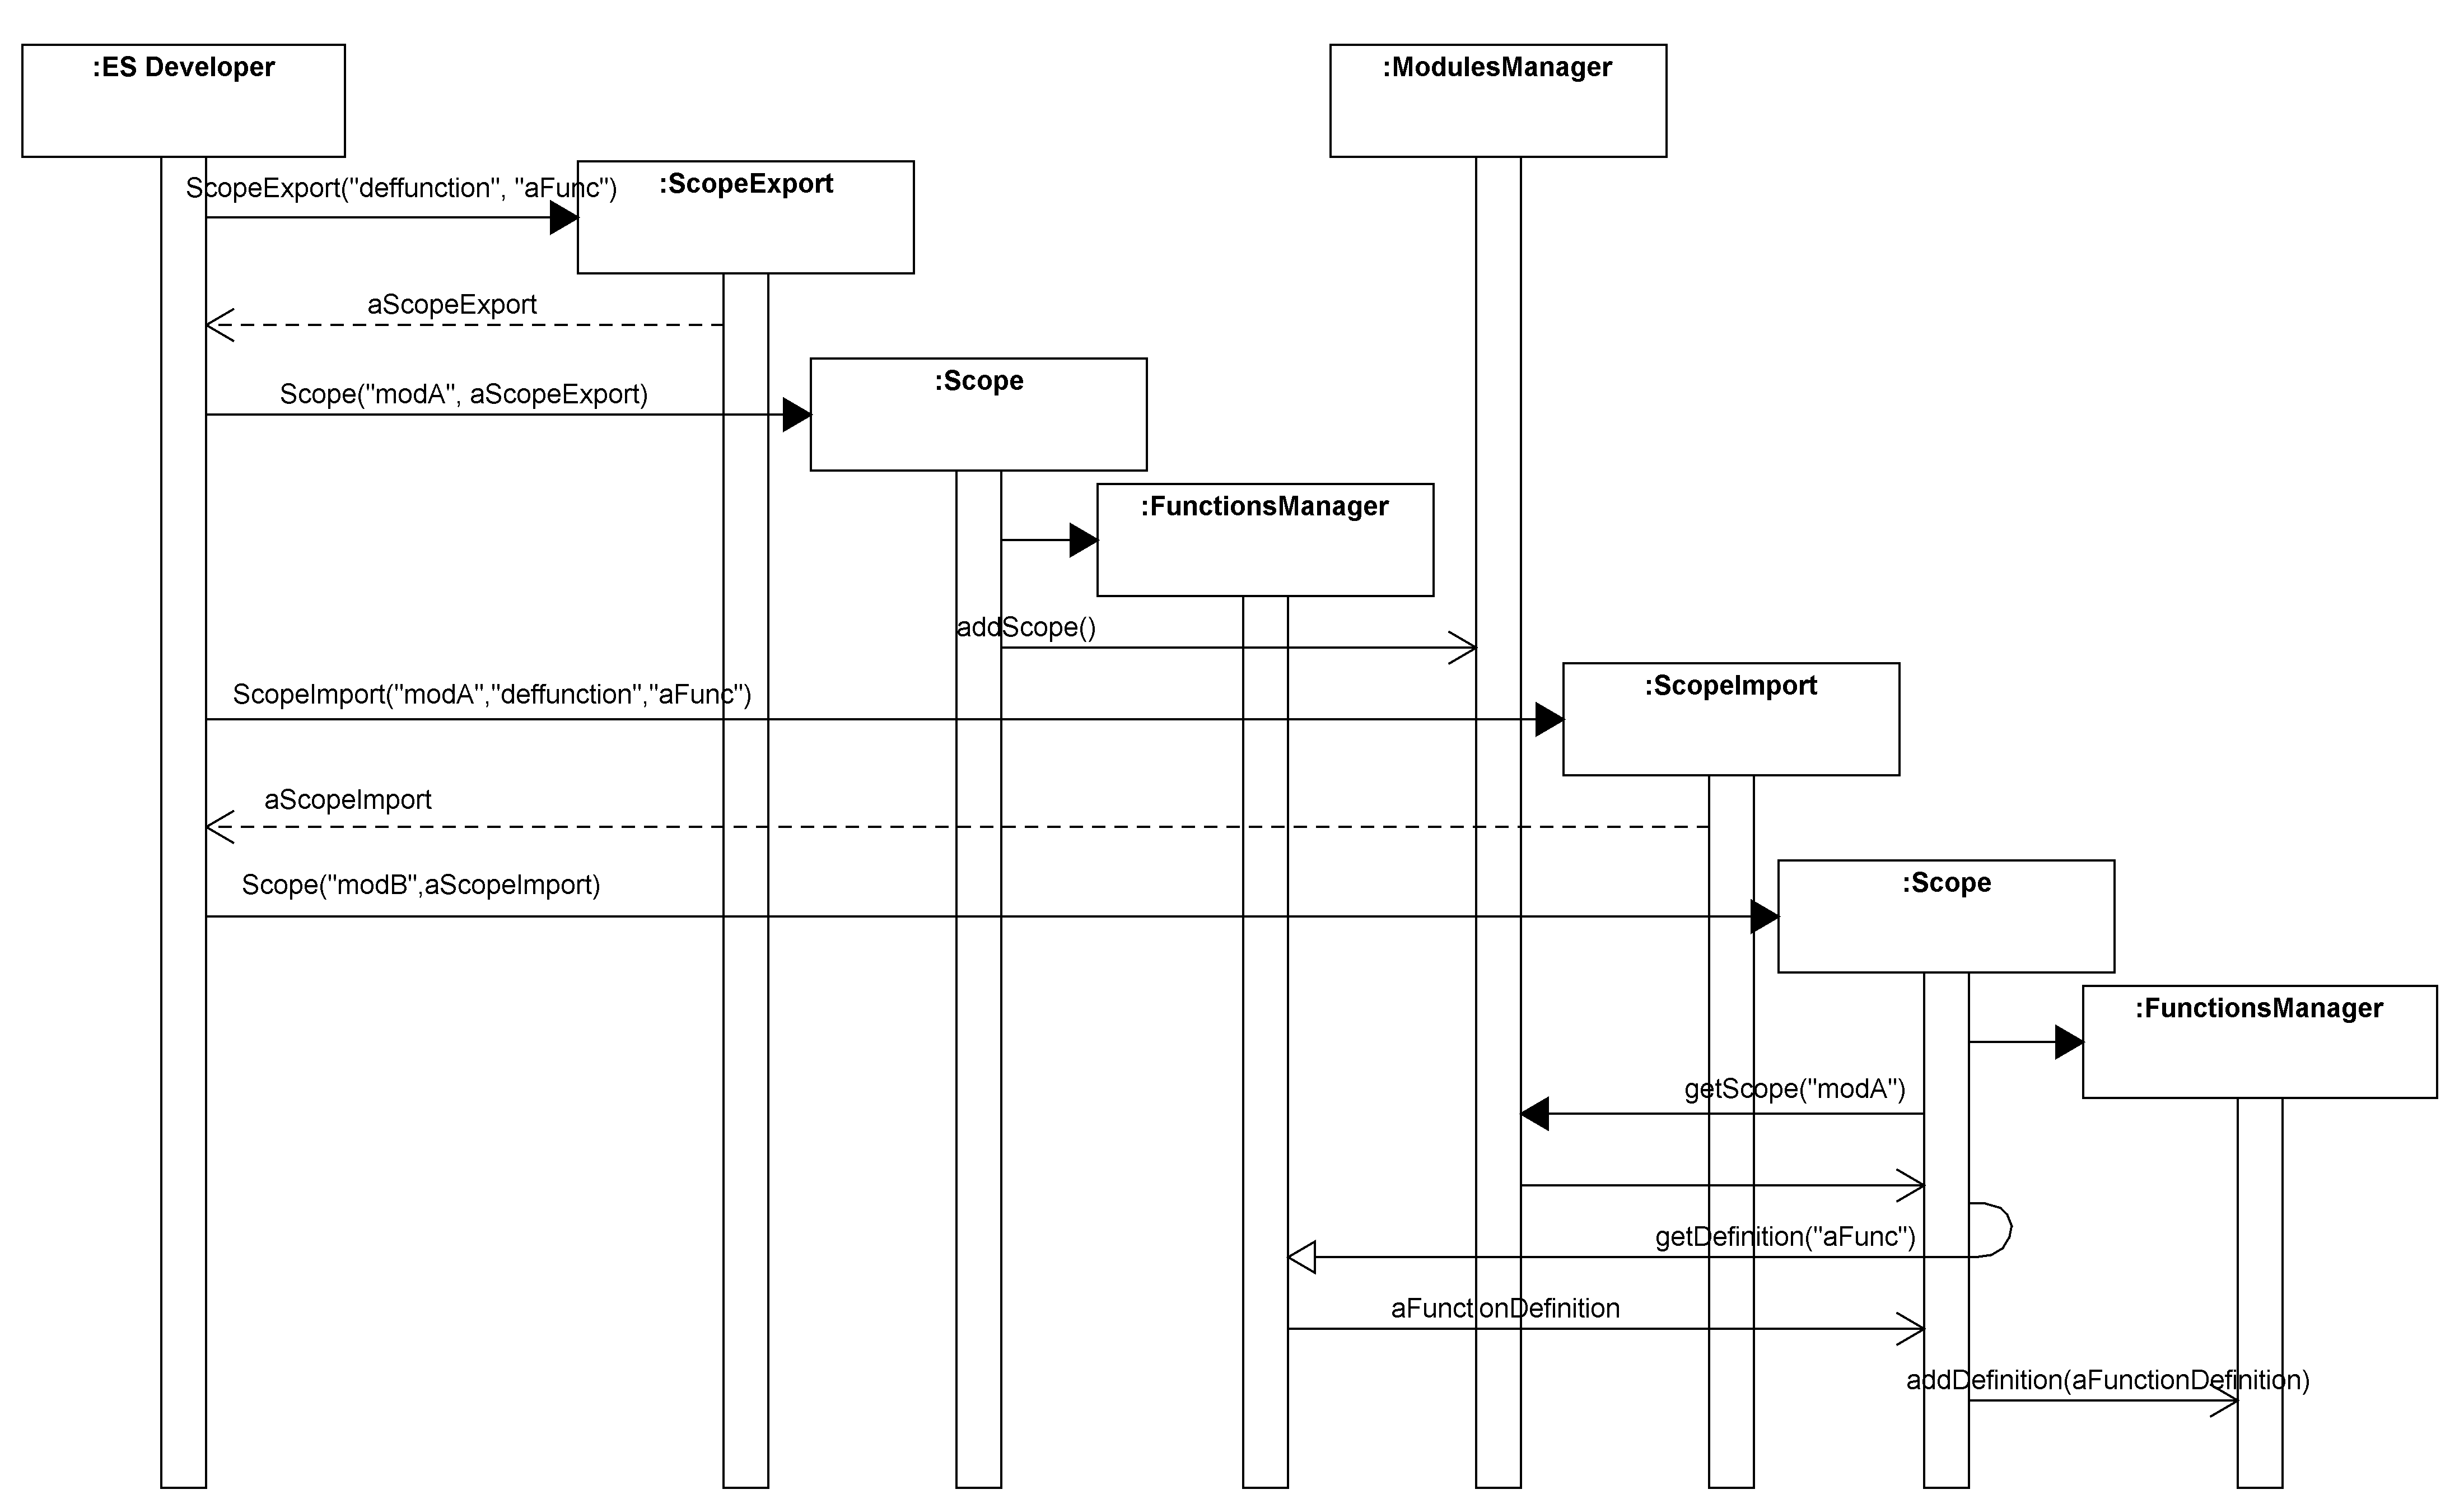
\includegraphics[width=1.2\textwidth, angle=270]{Immagini/Capitolo3/Sequenza/myclips_Scope_ImportExport.png}
\caption[Diagramma di sequenza \emph{import/export} delle definizioni]{Diagramma di sequenza \emph{import/export} delle definizioni: le clausule di importazione o esportazione determinano lo scambio di definizioni fra moduli}\label{fig:sequence-def-import-export}
\end{figure}

\begin{figure}
\centering
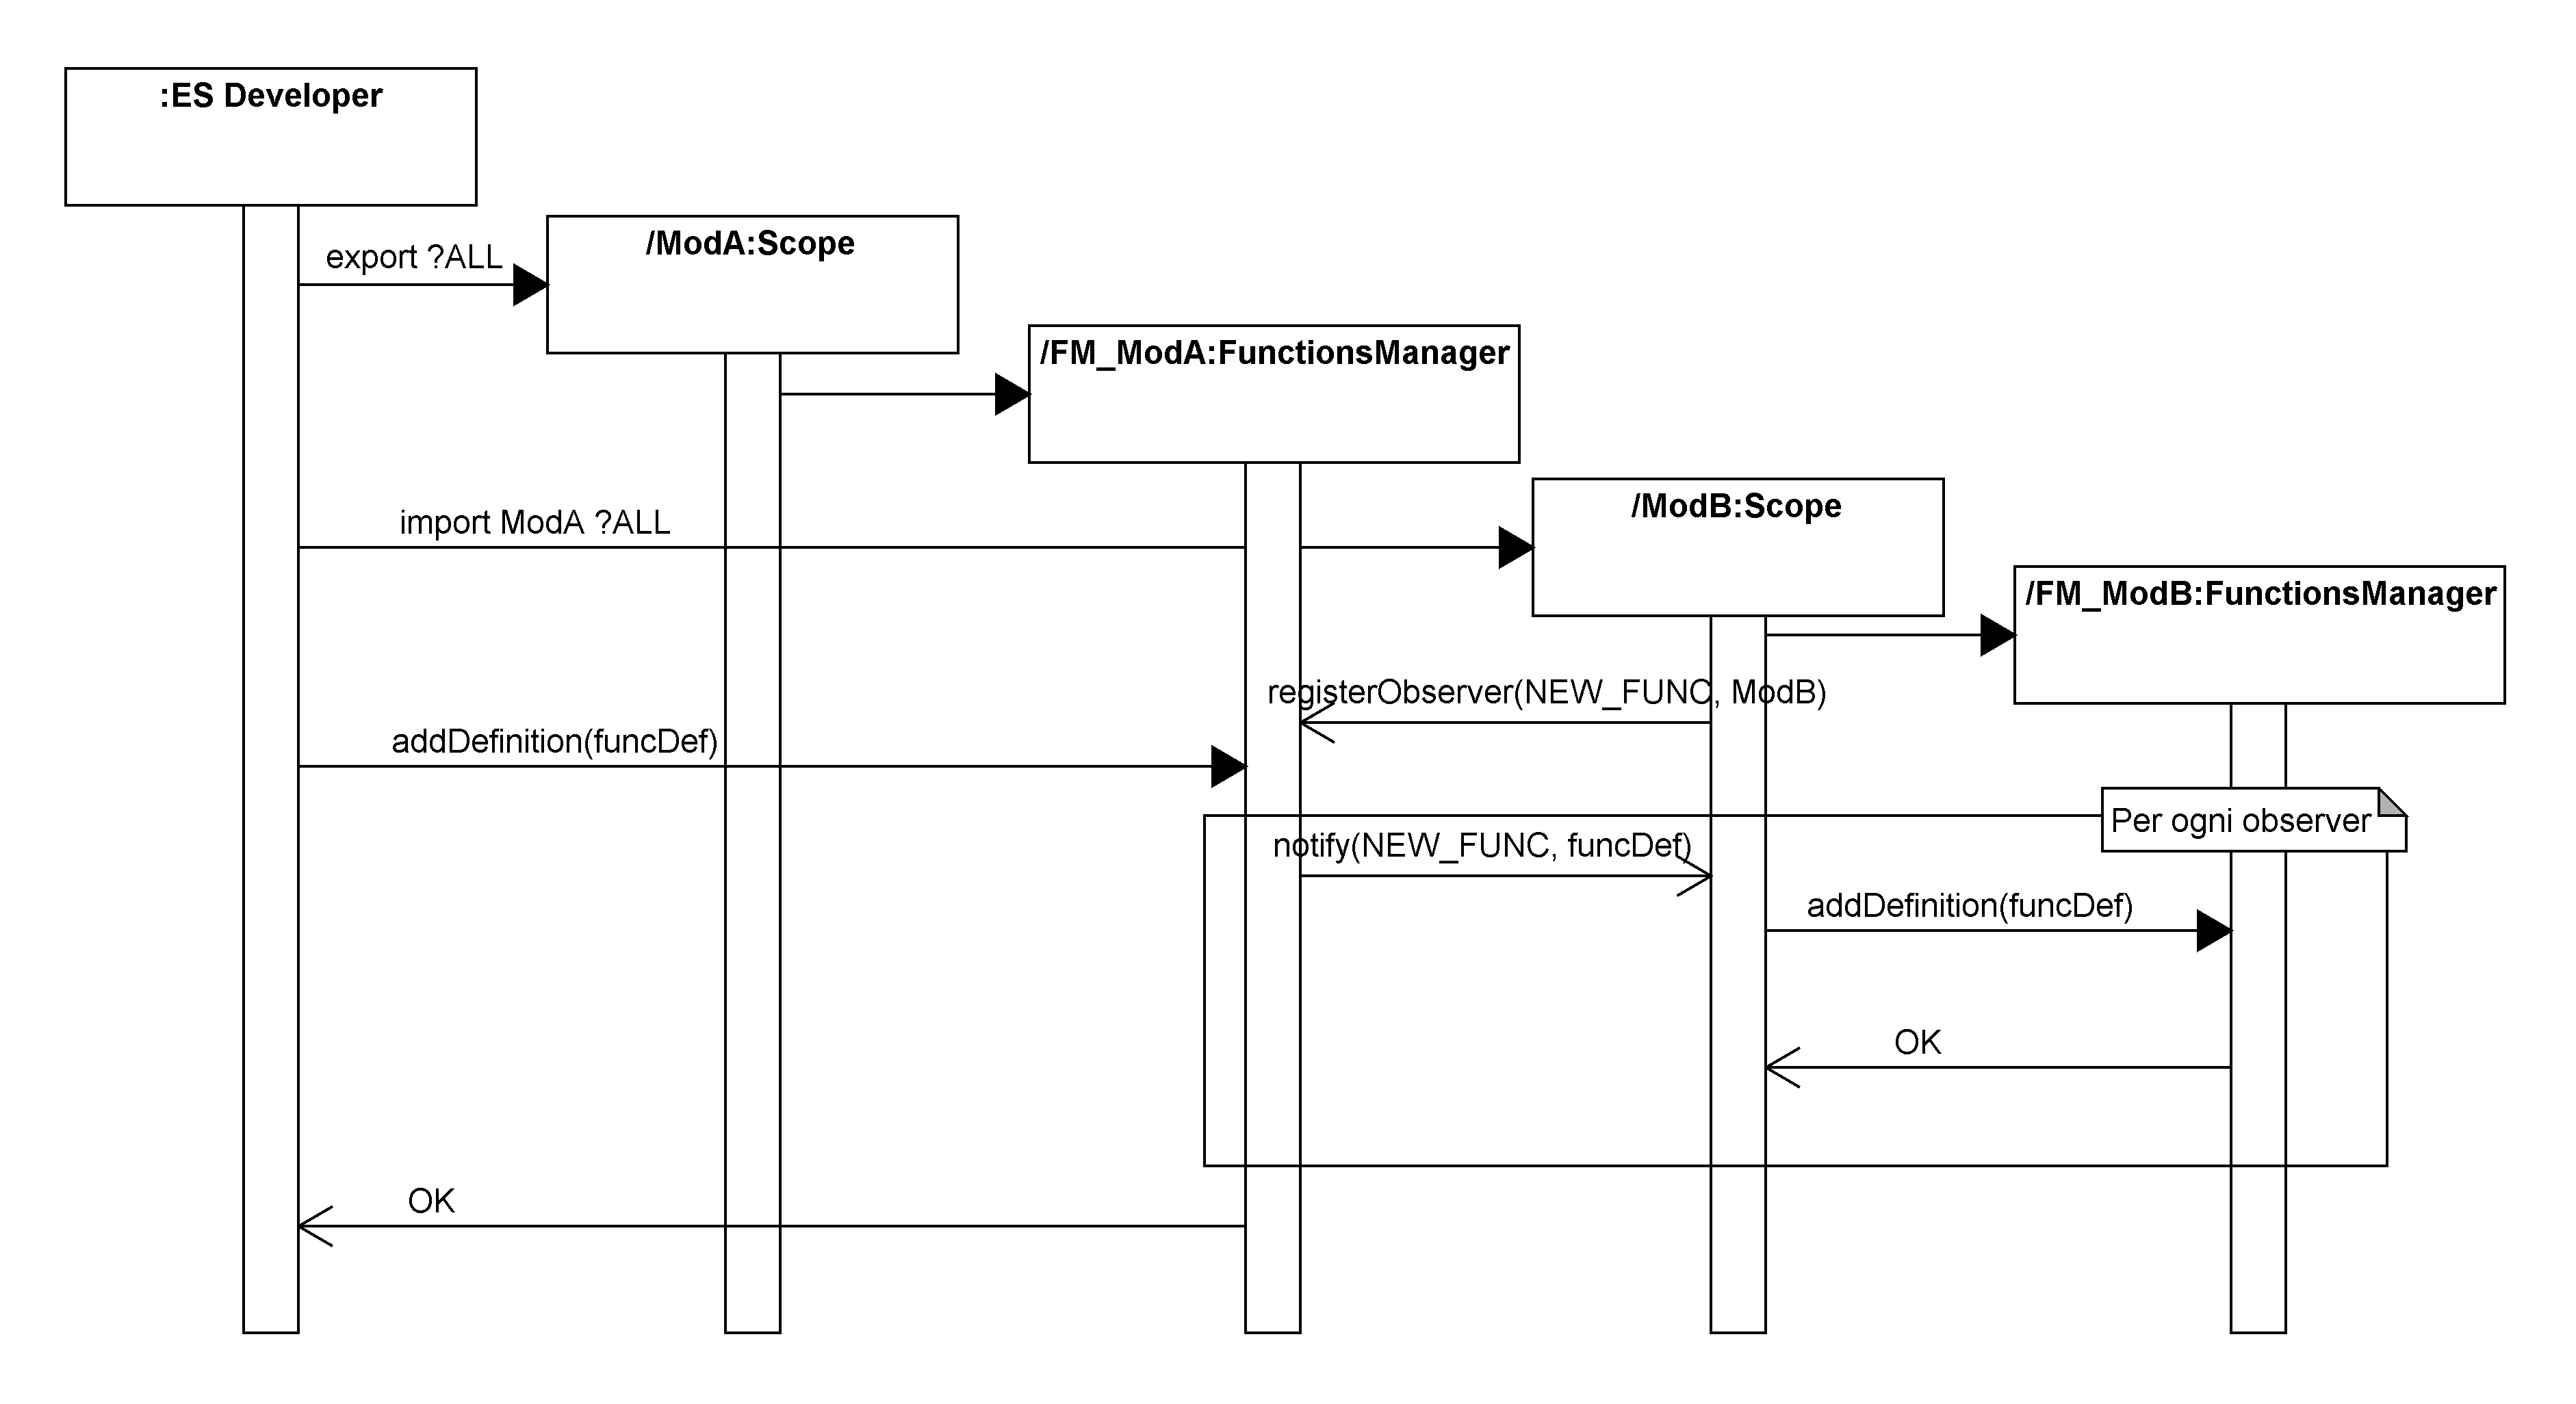
\includegraphics[width=1.3\textwidth, angle=270]{Immagini/Capitolo3/Sequenza/myclips_Scope_ExportPromise.png}
\caption[Diagramma di sequenza \emph{import/export} tramite l'uso di \emph{promesse}]{Diagramma di sequenza \emph{import/export} tramite l'uso di \emph{promesse}: i moduli vengono relazionati e l'aggiunta successiva di definizioni al primo modulo viene automaticamente inoltrata al secondo modulo}\label{fig:sequence-def-import-export-promise}
\end{figure}

Lo scambio di definizioni non ancora esplicitate avviene attraverso l'utilizzo delle \emph{promesse di import/export}. Nel momento in cui un modulo \emph{modA} definisce tutti i propri costrutti esportabili ed un secondo modulo \emph{modB} esplicita la volontà di importare tutti i costrutti di \emph{modA}, si fa uso di una \emph{promessa}: il protocollo prevede l'utilizzo di una soluzione basata sul pattern \emph{observer-observable} per eseguire il trasferimento delle definizioni aggiunte in fasi successive~(\figurename~\ref{fig:sequence-def-import-export-promise}).

\begin{figure}
\centering
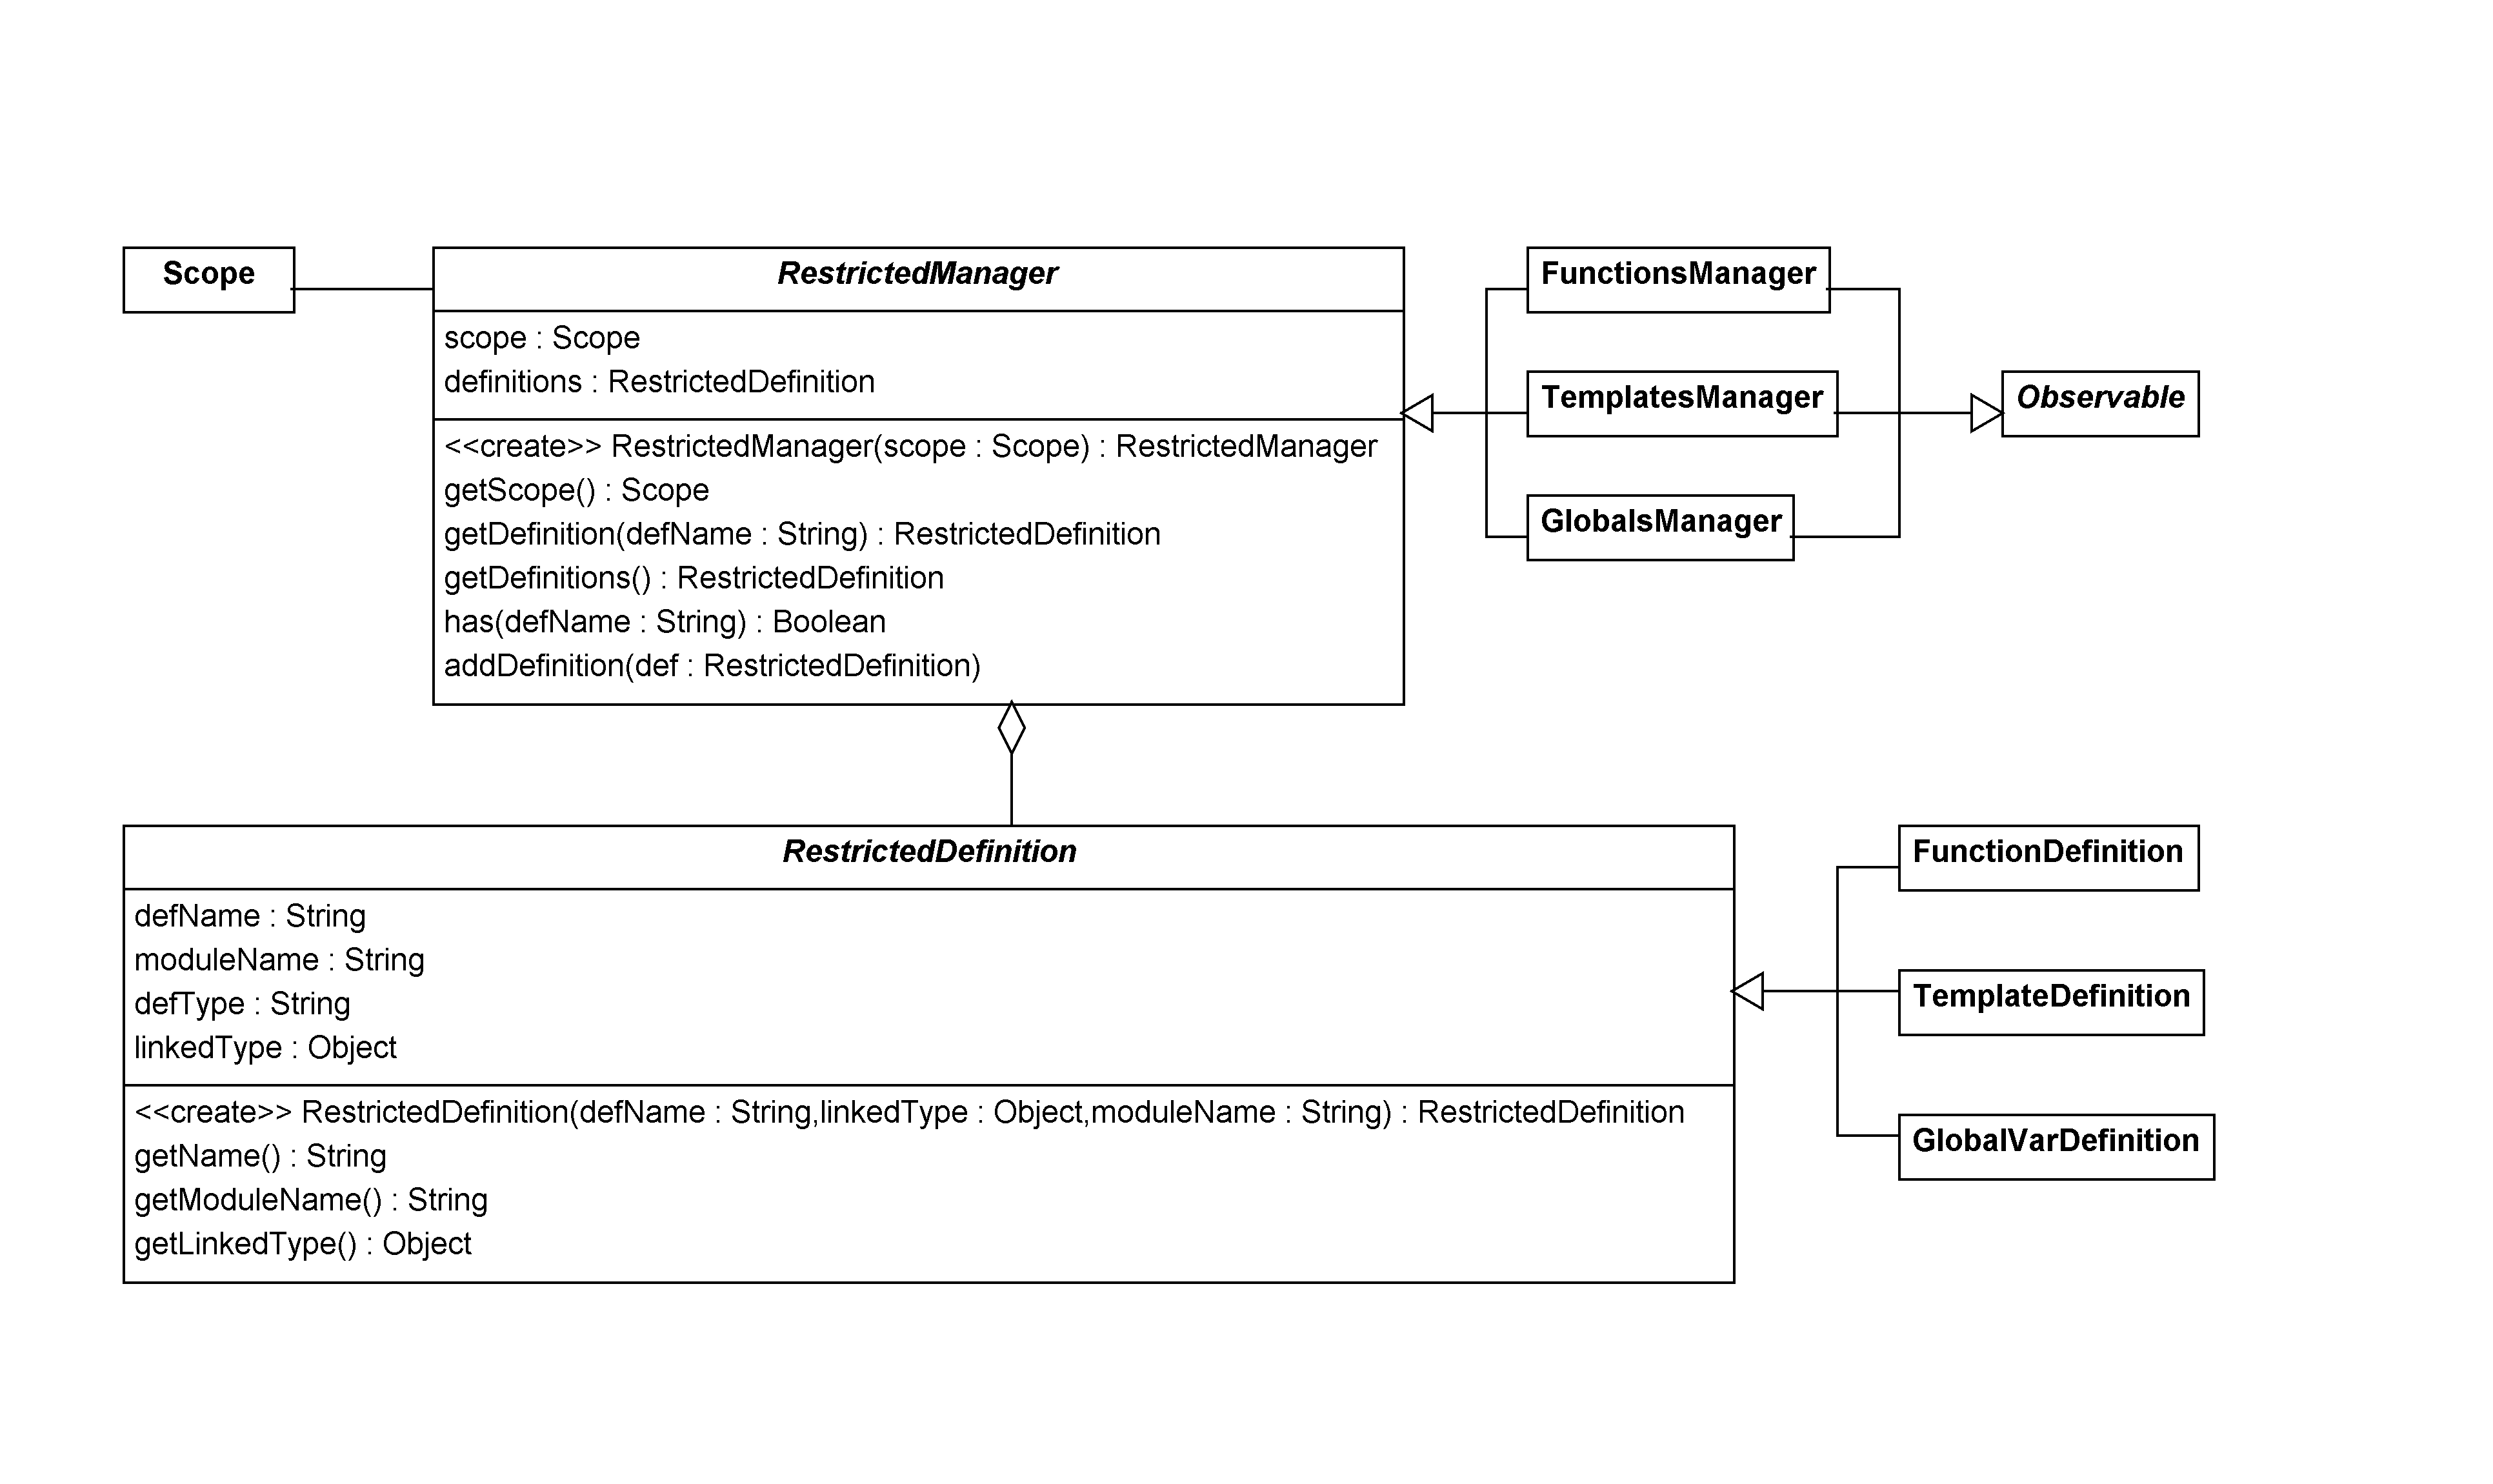
\includegraphics[width=1\textwidth]{Immagini/Capitolo3/Classi/myclips_RestrictedManager.png}
\caption{Vista delle classi \emph{manager} di definizioni}\label{fig:class-myclips-restricted-manager}
\end{figure}

La memorizzazione delle definizioni è affidata alle classi \emph{GlobalsManager}, \emph{TemplatesManager} e \emph{FunctionsManager}~(\figurename~\ref{fig:class-myclips-restricted-manager}). 
Ogni \emph{manager} memorizza un preciso tipo di definizioni che possono essere utilizzate nell'ambito di uno \emph{Scope} specifico. L'eventuale presenza di \emph{promesse di export} viene valutata durante l'aggiunta di nuove definizioni nei \emph{manager}~(\figurename~\ref{fig:sequence-def-import-export-promise}).


\paragraph{Gestione dell'inferenza}

\begin{figure}
\centering
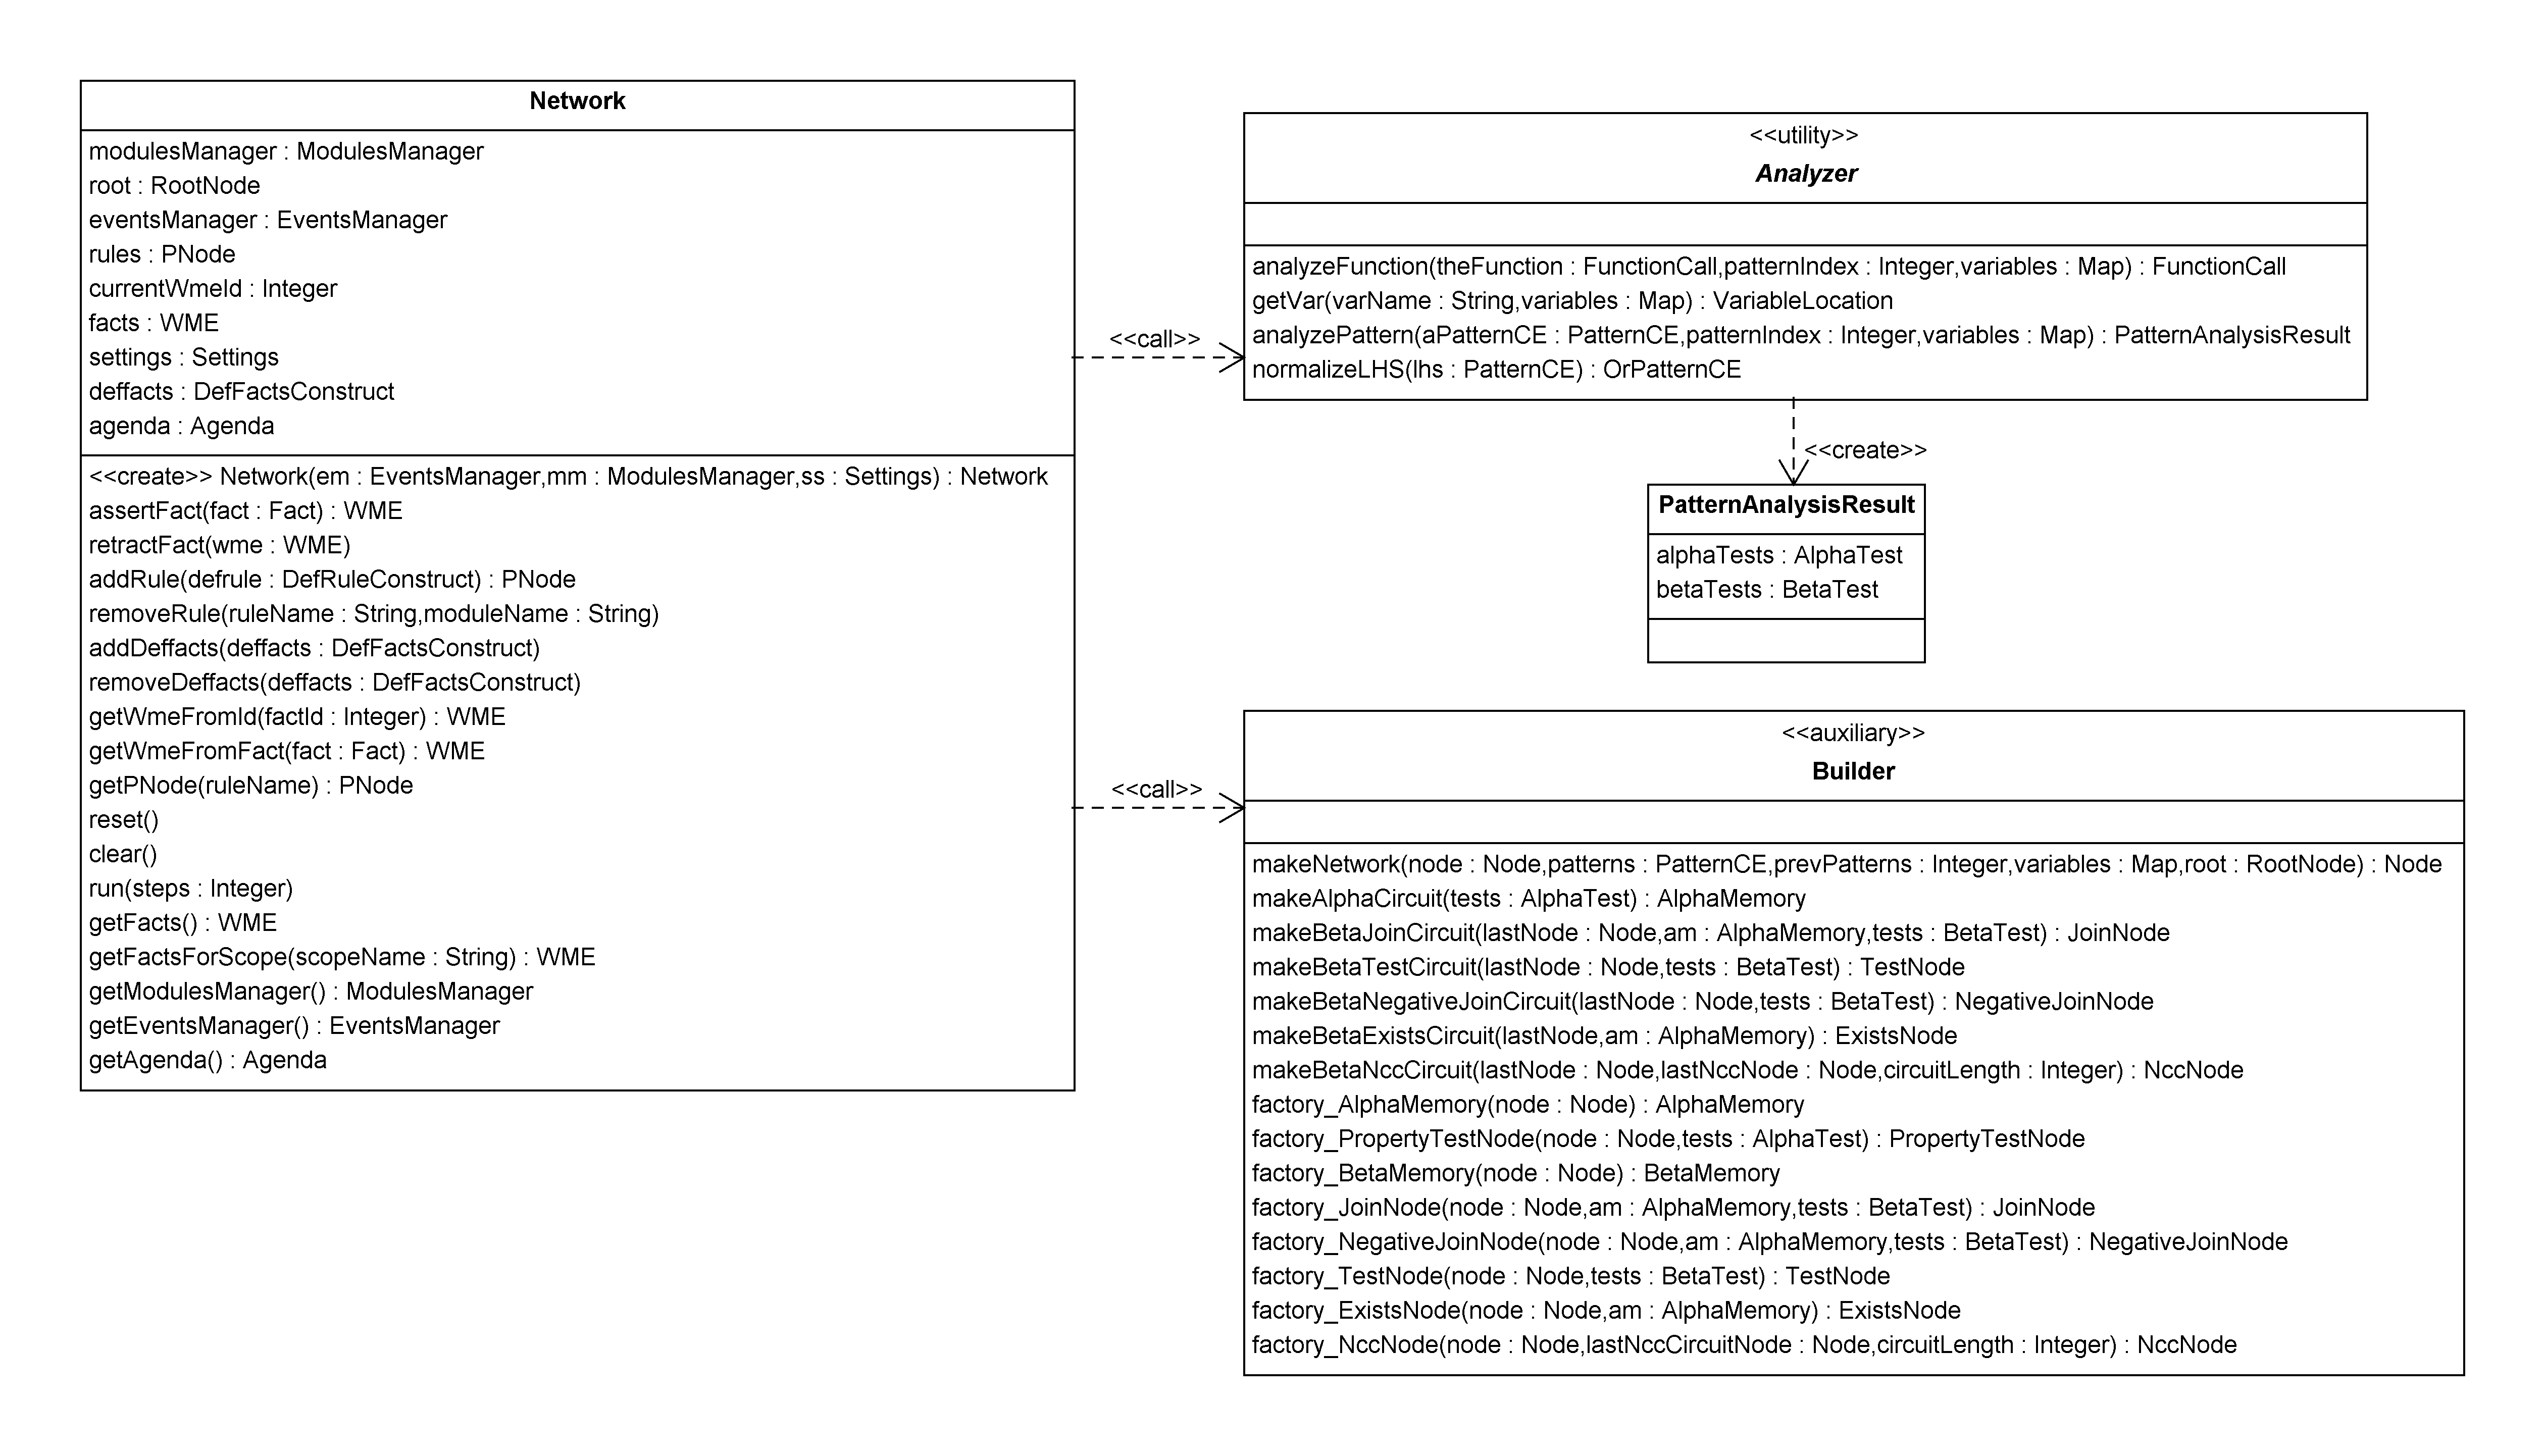
\includegraphics[width=1\textwidth]{Immagini/Capitolo3/Classi/myclips_rete_Network.png}
\caption{Package \emph{myclips}: vista della classe \emph{Network}}\label{fig:class-myclips-network}
\end{figure}

La classe principale per la gestione dell'inferenza è la classe \emph{fa\c{c}ade} \emph{Network}~(\figurename~\ref{fig:class-myclips-network}): astraendo dalla complessità delle interfacce offerte dal \emph{matcher}, offre metodi per la manipolazione del \emph{rules-set}, dei fatti iniziali e della \emph{working-memory}. Realizzando il ciclo \emph{recognize-act} al suo interno, permette l'utilizzo dei meccanismi di inferenza offerti dal sistema. La classe si affida a due componenti \emph{utility} per la reale implementazione delle funzionalità di compilazione e analisi delle regole interfacciandosi con il modulo \emph{matcher}, descritto in seguito.


\begin{figure}
\centering
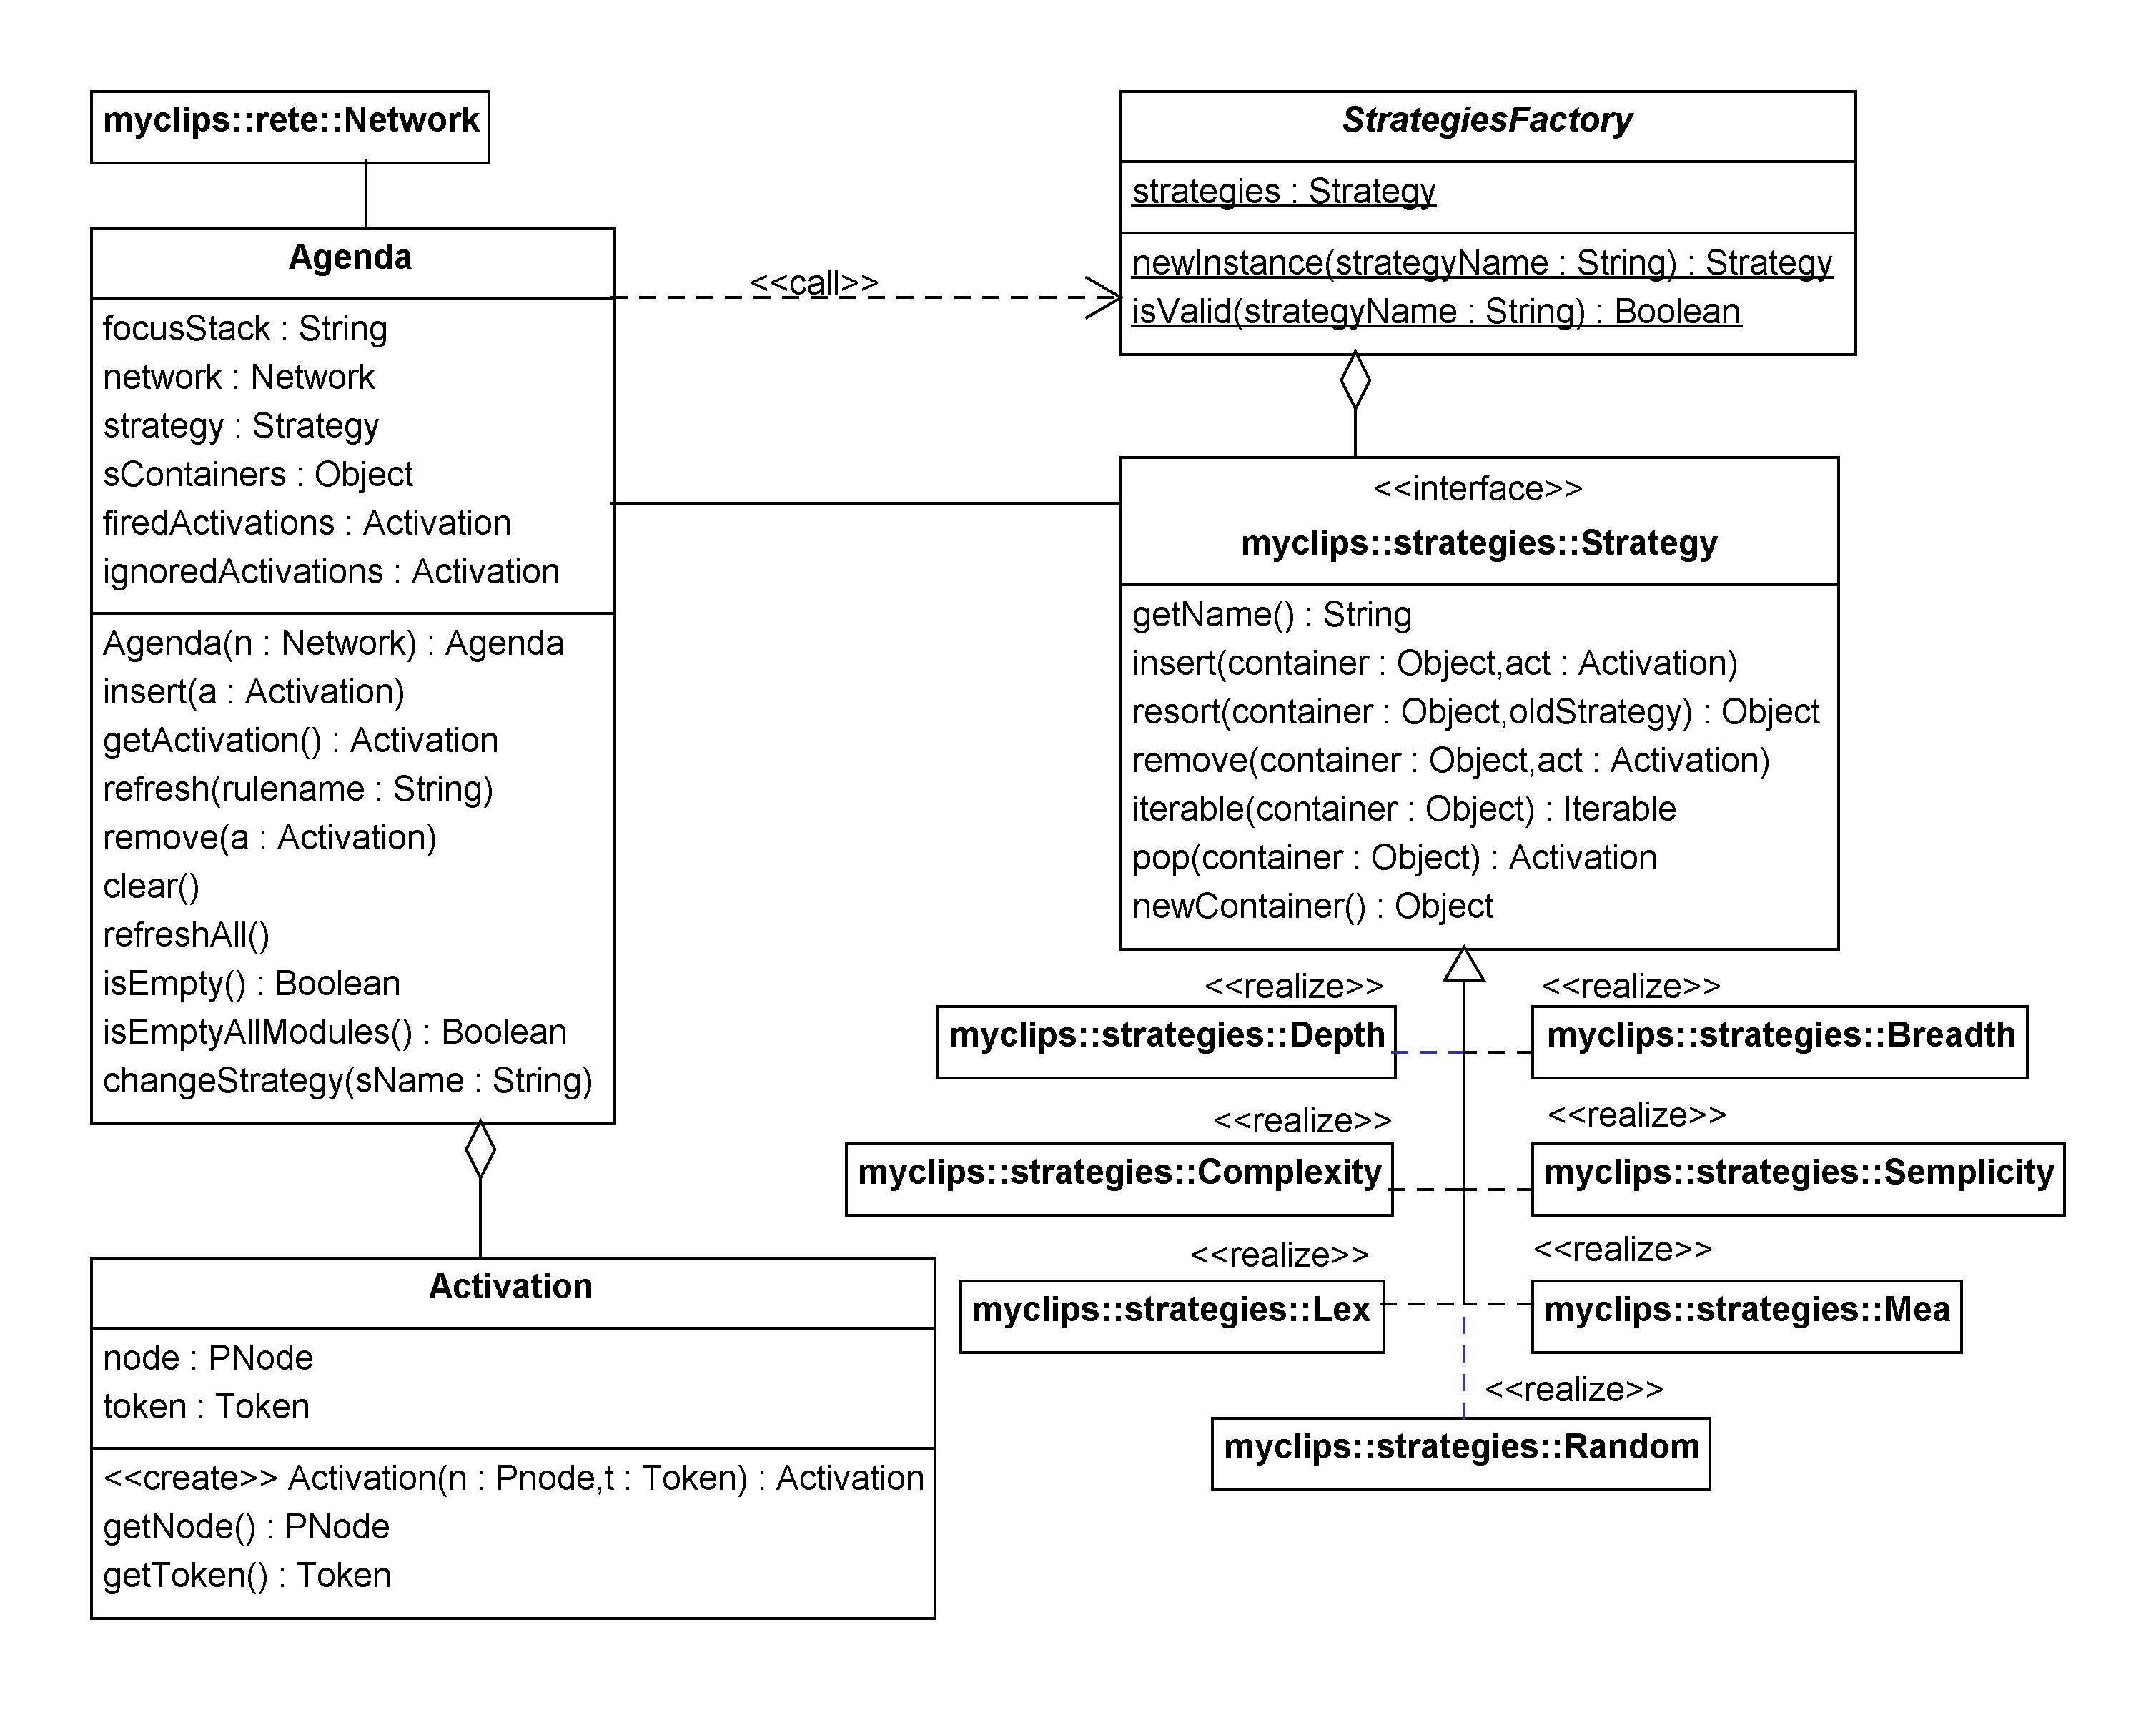
\includegraphics[width=1\textwidth]{Immagini/Capitolo3/Classi/myclips_Agenda-Strategies.png}
\caption{Package \emph{myclips}: vista delle classi e interfacce relative ad  \emph{Agenda} e \emph{Strategie} (CRS)}\label{fig:class-myclips-agenda-strategies}
\end{figure}

La gestione delle attivazioni viene affidata alla classe \emph{Agenda} e al \emph{package} \emph{myclips.strategies}~(\figurename~\ref{fig:class-myclips-agenda-strategies}). La classe organizza le attivazioni, offrendo servizi per l'aggiunta o la rimozione delle stesse, e gestendo le strategie di risoluzione dei conflitti. La collaborazione fra \emph{Agenda} e \emph{Strategy} viene realizzata attraverso l'utilizzo del pattern \emph{Factory}: la creazione dell'istanza di strategia viene delegata ad una istanza \emph{Singleton} della classe \emph{StrategiesFactory}, la quale inizializza un'implementazione dell'interfaccia \emph{Strategy} fornita basandosi su un id di strategia. L'implementazione dell'\emph{Agenda} viene realizzata tenendo conto dei metodi forniti dall'interfaccia, astraendo dall'implementazione concreta. Le strutture dati adibite alla memorizzazione delle sequenze di attivazioni vengono inizializzate e concretamente gestite dalla specifica implementazione della \emph{Strategy}.


\subsubsection{Modulo Matcher}
Lo scopo del modulo \emph{matcher} è quello di confrontare lo stato della \emph{working-memory} con il \emph{rule-set}, identificando l'insieme di attivazioni disponibili e inserendole nell'\emph{agenda delle attivazioni}.

\begin{figure}
\centering
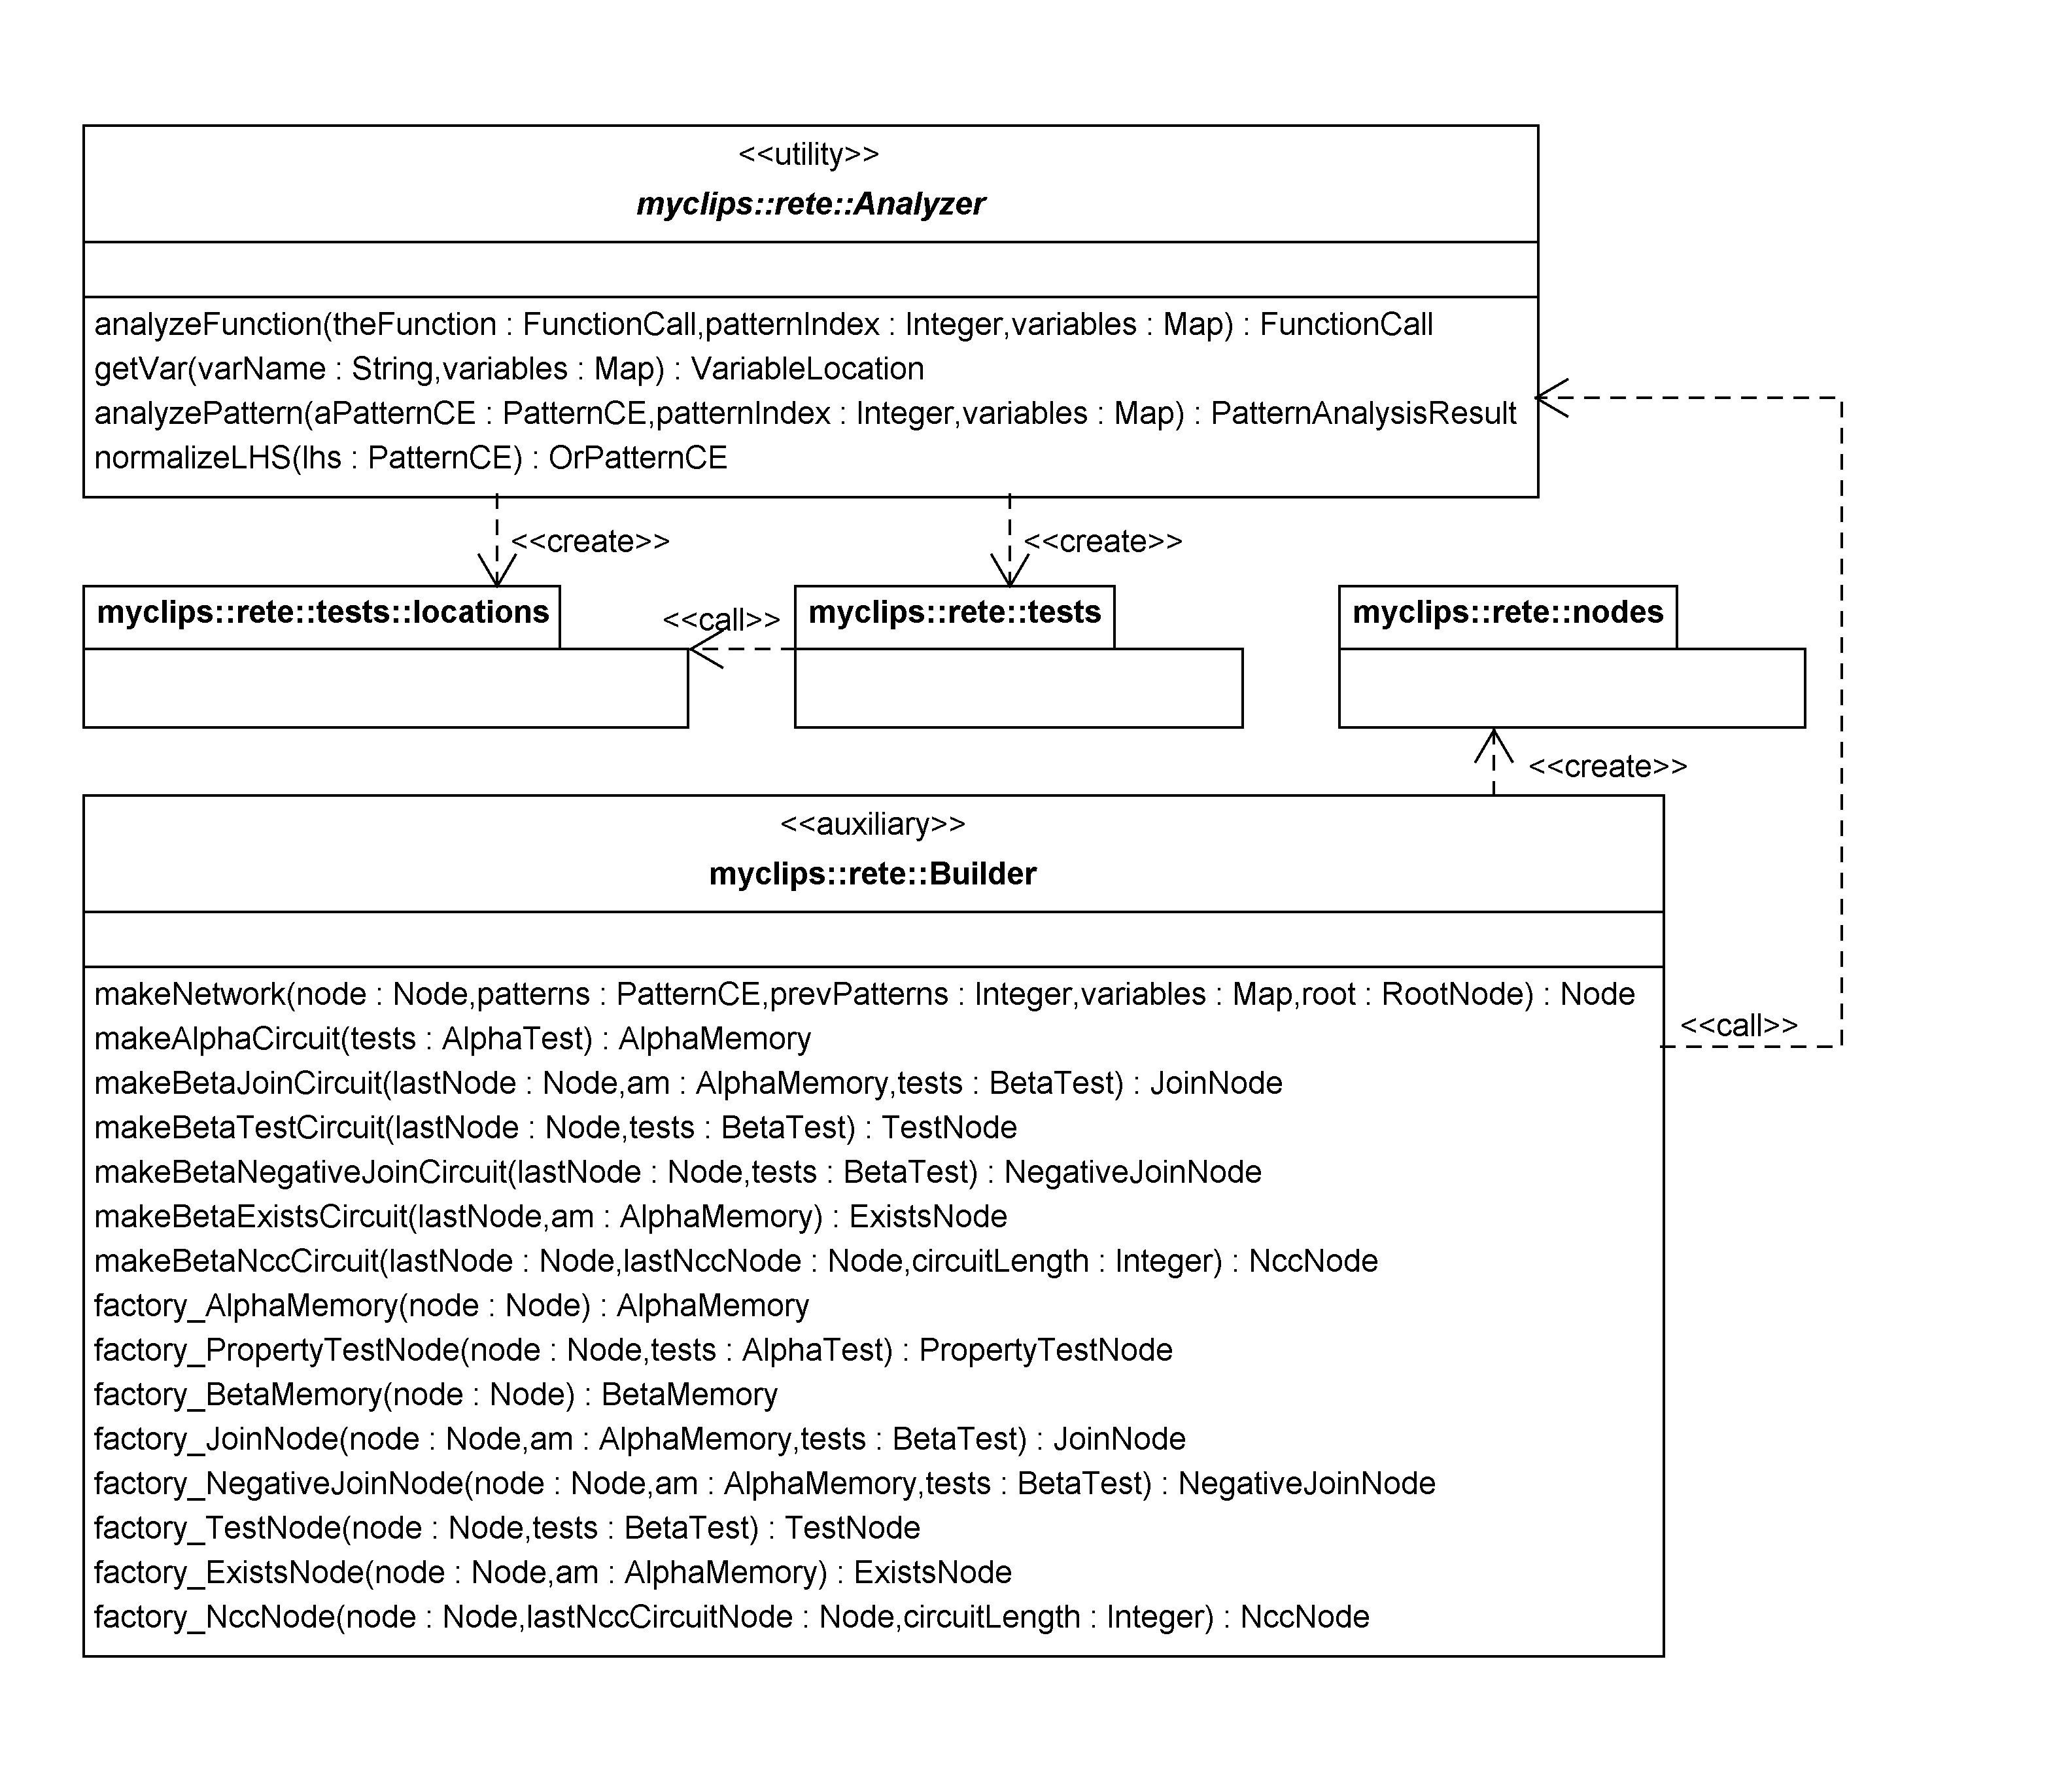
\includegraphics[width=1\textwidth]{Immagini/Capitolo3/Classi/myclips_rete_Builders.png}
\caption{Package \emph{myclips.rete}: vista delle classi utility per la conversione delle regole in strutture di RETE}\label{fig:class-myclips-rete-builders}
\end{figure}

Il modulo si basa sull'utilizzo di un'implementazione interpretata dell'algoritmo RETE. Attraverso l'uso di due classi utility~(\figurename~\ref{fig:class-myclips-rete-builders}), per l'analisi dei \emph{pattern} delle regole e per la costruzione del grafo, il \emph{rules-set} viene convertito nel grafo esplicito di valutazione caratteristico dell'algoritmo RETE.

La classe \emph{Analyzer} viene utilizzata per manipolare la forma dei pattern delle regole nel \emph{rules-set}, adattandole alla topologia del grafo di RETE, e individuare l'insieme dei test \emph{alpha} e \emph{beta} per i pattern, inizializzando le relative istanze delle classi di test organizzate nel package \emph{myclips.rete.tests}.

La classe \emph{Builder} ha invece il compito di creare l'insieme di nodi necessari alla costituzione del grafo, associandoli dove necessario ai test ottenuti dall'\emph{Analyzer}.
L'utilizzo dei metodi \emph{factory} per i nodi, come alternativa a normali costruttori, permette di utilizzare istanze condivise dei nodi quando possibile.

\paragraph{Compilazione delle regole}

L'algoritmo utilizzato per la compilazione delle regole segue quanto proposto in \cite{Doorenbos95productionmatching}, con alcune modifiche per permette l'utilizzo di pattern non previsti in origine come \emph{or-CE}, \emph{exists-CE} e \emph{test-CE}.

La procedura principale di compilazione ha inizio all'interno del metodo \emph{Network::addRule}: utilizzando \emph{Analyzer}, l'insieme dei pattern della regola vengono trasformati in modo che l'insieme di condizioni sia presentato in una forma normalizzata dove il primo pattern sia un elemento \emph{or-CE} con al suo interno almeno un elemento \emph{and-CE} che racchiuda le condizioni originali. Durante la normalizzazione, l'eventuale presenza di condizioni \emph{or} poste all'interno dei pattern viene trasferita nella radice della nuova \emph{LHS} normalizzata.



\begin{algorithm}
\caption{Compilazione di una regola}\label{alg:builder-makeNetwork}
\begin{algorithmic}
\Function{Builder.makeNetwork}{parent: node, conds: \textbf{list} of conditions, prevConds: integer}
\State \textbf{siano} $c_1,\dots,c_k$ le componenti di conds
\For{$i = 1 \to k$}
	\If {$c_i$ is-a Pattern-CE}
	    \State $tests_\alpha\gets$ Analysis.analyzePattern($c_i$, $\alpha$)
	    \State $memory_\alpha\gets$ Builder.makeAlphaCircuit($tests_\alpha$)
	    \State $tests_\beta\gets$ Analysis.analyzePattern($c_i$, $\beta$)
	    \State $parent\gets$ Builder.makeJoinCircuit($parent$, $memory_\alpha$, $tests_\beta$)
	\ElsIf {$c_i$ is-a Not-CE}
	    \State $tests_\alpha\gets$ Analysis.analyzePattern($c_i$, $\alpha$)
	    \State $memory_\alpha\gets$ Builder.makeAlphaCircuit($tests_\alpha$)
	    \State $tests_\beta\gets$ Analysis.analyzePattern($c_i$, $\beta$)
	    \State $parent\gets$ Builder.makeNegativeJoinCircuit($parent$, $memory_\alpha$, $tests_\beta$)
	\ElsIf {$c_i$ is-a Ncc-CE}
		\State \textbf{siano} $ncc_i$ le componenti negate da $c_i$
		\State \textbf{sia} $l$ il numero di componenti in $ncc_i$
	    \State $lastNccNode\gets$ Builder.makeNetwork($parent$, $ncc_i$, $prevConds$)
	    \State $node\gets$ Builder.makeNccCircuit($parent$, $lastNccNode$, $l$)
	\ElsIf {$c_i$ is-a Test-CE}
		\State $tests_\theta\gets$ Analysis.analyzePattern($c_i$, $\theta$)
		\State $parent\gets$ Builder.makeTestCircuit($parent$, $tests_\theta$)	
	\ElsIf {$c_i$ is-a Exists-CE}
	    \State $tests_\alpha\gets$ Analysis.analyzePattern($c_i$, $\alpha$)
	    \State $memory_\alpha\gets$ Builder.makeAlphaCircuit($tests_\alpha$)
	    \State $tests_\beta\gets$ Analysis.analyzePattern($c_i$, $\beta$)
	    \State $parent\gets$ Builder.makeExistsCircuit($parent$, $memory_\alpha$, $tests_\beta$)
	\EndIf
	\State $prevConds\gets prevConds + 1$
\EndFor
\State \Return{$node$}
\EndFunction
\end{algorithmic}
\end{algorithm}



Ogni gruppo di condizioni \emph{and-CE} genera un nuovo circuito indipendente. La compilazione del circuito ha luogo all'interno del metodo \emph{Builder::makeNetwork}~(Algoritmo~\ref{alg:builder-makeNetwork}): viene verificato il tipo di ogni pattern e quindi avviata la procedura di compilazione più indicata per lo stesso.



\begin{algorithm}
\caption{Creazione di un circuito $\alpha$}\label{alg:builder-makeAlpha}
\begin{algorithmic}
\Function{Builder.makeAlphaCircuit}{$tests_\alpha$: \textbf{list} of test}
\State \textbf{siano} $t_1,\dots,t_k$ le componenti di $tests_\alpha$
\State \textbf{sia} $root$ il nodo radice del grafo di RETE
\State $lastNode\gets root$
\For{$i = 1 \to k$}
	\State $lastNode\gets$ Builder.factory\_PropertyTestNode($lastNode$, $t_i$)
\EndFor
\State $lastNode\gets$ Builder.factory\_AlphaMemory($lastNode$)
\State \Return{$lastNode$}
\EndFunction
\end{algorithmic}
\end{algorithm}



\begin{algorithm}
\caption{Creazione di un circuito $\beta$ per il Join}\label{alg:builder-makeJoin}
\begin{algorithmic}
\Function{Builder.makeBetaJoinCircuit}{parent: node, $memory_\alpha$: node, $tests_\beta$: \textbf{list} of test}
\State $parent\gets$ Builder.factory\_BetaMemory($parent$)
\State $parent\gets$ Builder.factory\_JoinNode($parent$, $memory_\alpha$, $tests_\beta$)
\State \Return{$parent$}
\EndFunction
\end{algorithmic}
\end{algorithm}




Ad ogni tipo di pattern corrisponde una procedura apposita. Nel caso più comune, un normale \emph{Pattern-CE}, questo viene prima analizzato per l'identificazione dei test \emph{alpha} e \emph{beta}: i primi vengono utilizzati per la generazione di un circuito che filtri gli elementi della \emph{working-memory} in base ai criteri del pattern~(Algoritmo~\ref{alg:builder-makeAlpha}), mentre quelli \emph{beta} per la creazione di un nodo \emph{Join} che riunisca il circuito \emph{alpha} appena creato con le porzioni \emph{beta} della regola create in precedenza~(Algoritmo~\ref{alg:builder-makeJoin}).


\begin{algorithm}
\caption{Esempio di metodo \emph{factory} per i nodi}\label{alg:builder-factory}
\begin{algorithmic}
\Function{Builder.factory}{nodeType: un tipo di nodo, parent: node, params: \textbf{list} of parametri di creazione del nodo}
\State \textbf{siano} $child_1,\dots,child_k$ i nodi successori di $parent$
\For{$i = 1 \to k$}
	\State \textbf{siano} $params_{child_i}$ i parametri di creazioni usati per il nodo $child_i$
	\If {$child_i$ is-a $nodeType$ $\wedge$ $params = params_{child_i}$}
		\State \Return{$child_i$}
	\EndIf
\EndFor
\State \textbf{sia} $newNode$ un nuovo nodo di tipo $nodeType$ creato con i parametri $params$
\State aggiungi $newNode$ fra i successori di $parent$
\State imposta $parent$ come padre di $newNode$
\State \Return{$newNode$}
\EndFunction
\end{algorithmic}
\end{algorithm}


La procedura di generazione dei nodi~(Algoritmo~\ref{alg:builder-factory}) controlla prima la possibilità di condividere un nodo già esistente che verifichi condizioni analoghe a quelle desiderate, quindi provvede alla creazione di una nuova istanza nel caso la condivisione non sia possibile. La possibilità di condividere un nodo precedentemente creato dipende sia dall'esistenza di un nodo di tipo analogo a quello desiderato, sia dall'effettiva corrispondenza fra i test eseguiti dal nodo esistente con quelli che si desidera eseguiti dal nuovo nodo.



\paragraph{Nodi del grafo di RETE}

Il set di nodi che supportano l'implementazione dell'algoritmo RETE sono realizzazioni di un set di interfacce fondamentali (\figurename~\ref{fig:class-myclips-rete-interfaces}) che hanno il compito di formalizzare i metodi usati dai nodi per lo scambio di segnali e rendere possibile l'attraversamento da parte dei \emph{Token}.

\begin{figure}
\centering
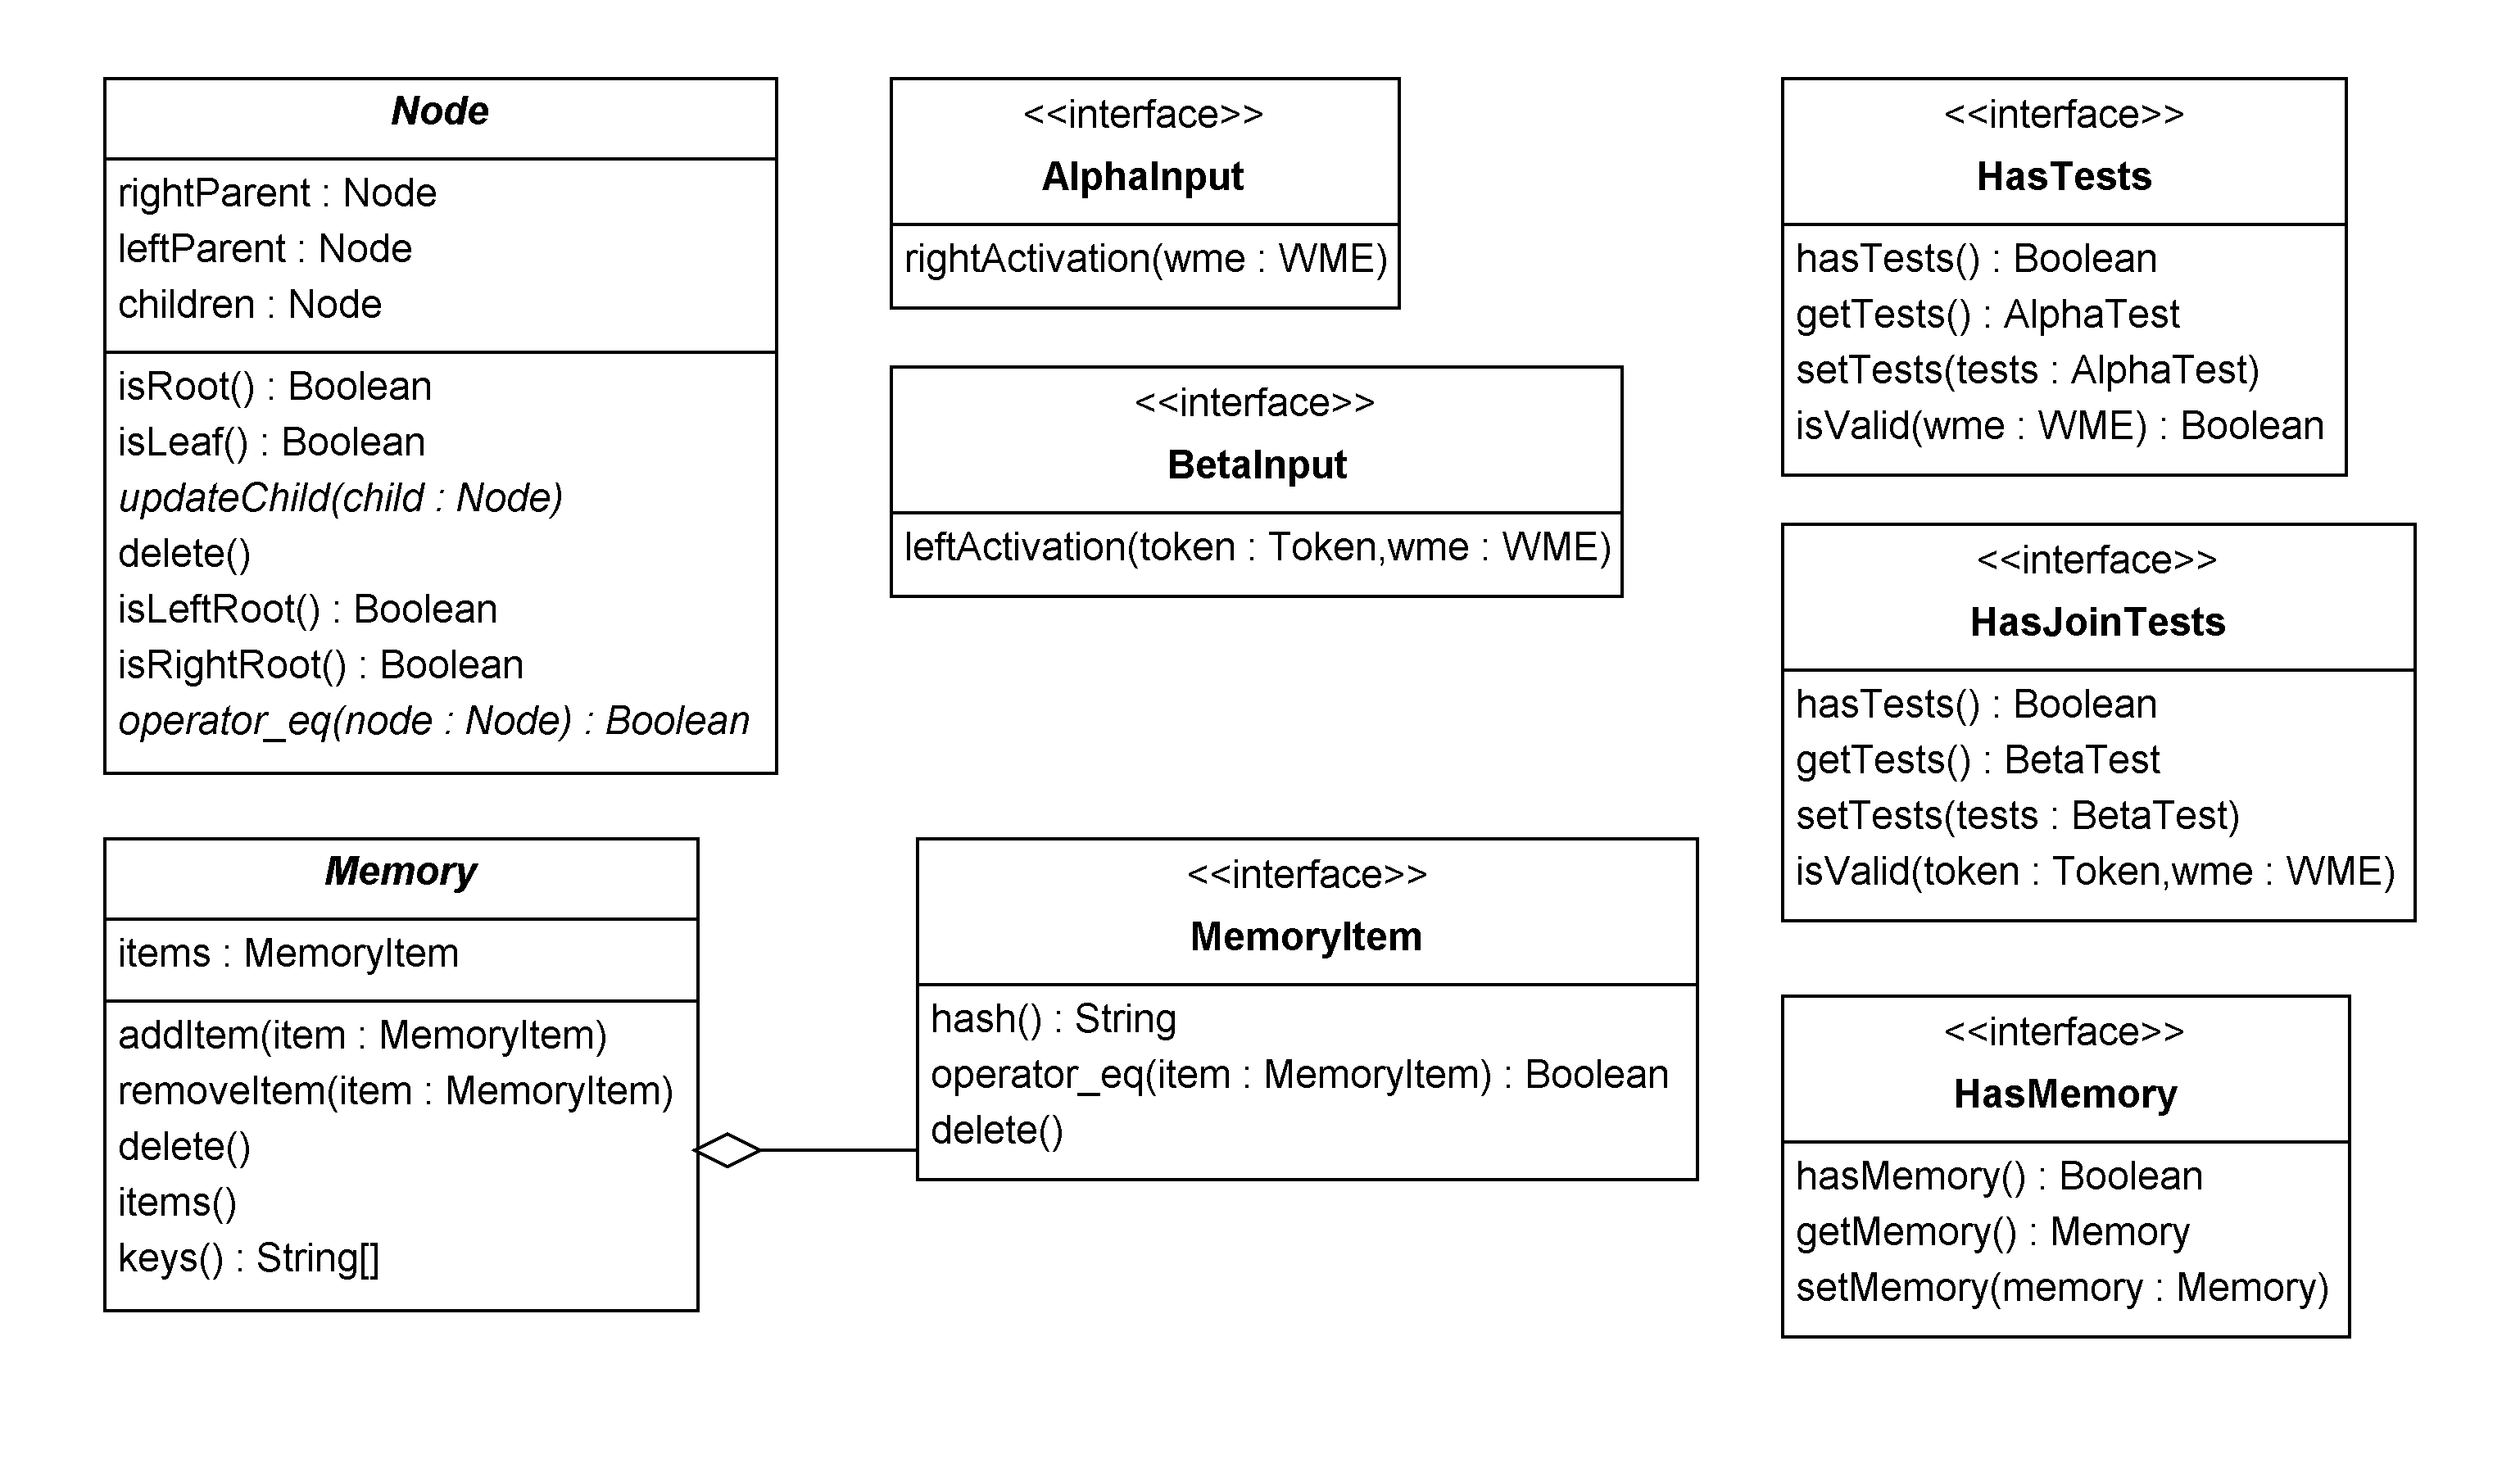
\includegraphics[width=1\textwidth]{Immagini/Capitolo3/Classi/myclips_rete_Interfacce.png}
\caption{Package \emph{myclips.rete}: vista delle interfacce di base usate dai nodi per l'implementazione di RETE}\label{fig:class-myclips-rete-interfaces}
\end{figure}

La classe astratta \emph{Node}, specializzata da tutti i nodi, rappresenta la struttura di base comune a tutti i tipi: memorizza i riferimenti ai nodi padre (destro per tutti i nodi, sinistro solo per quelli a due input) e i riferimenti ai nodi successori. Le memorie, \emph{alpha} e \emph{beta}, ed i nodi che memorizzano attivazioni parziali estendono inoltre la classe \emph{Memory}. Le ulteriori interfacce presenti in \figurename~\ref{fig:class-myclips-rete-interfaces} formalizzano i metodi relativi all'esecuzione dei test e alla propagazione delle attivazioni parziali.

\begin{figure}
\centering
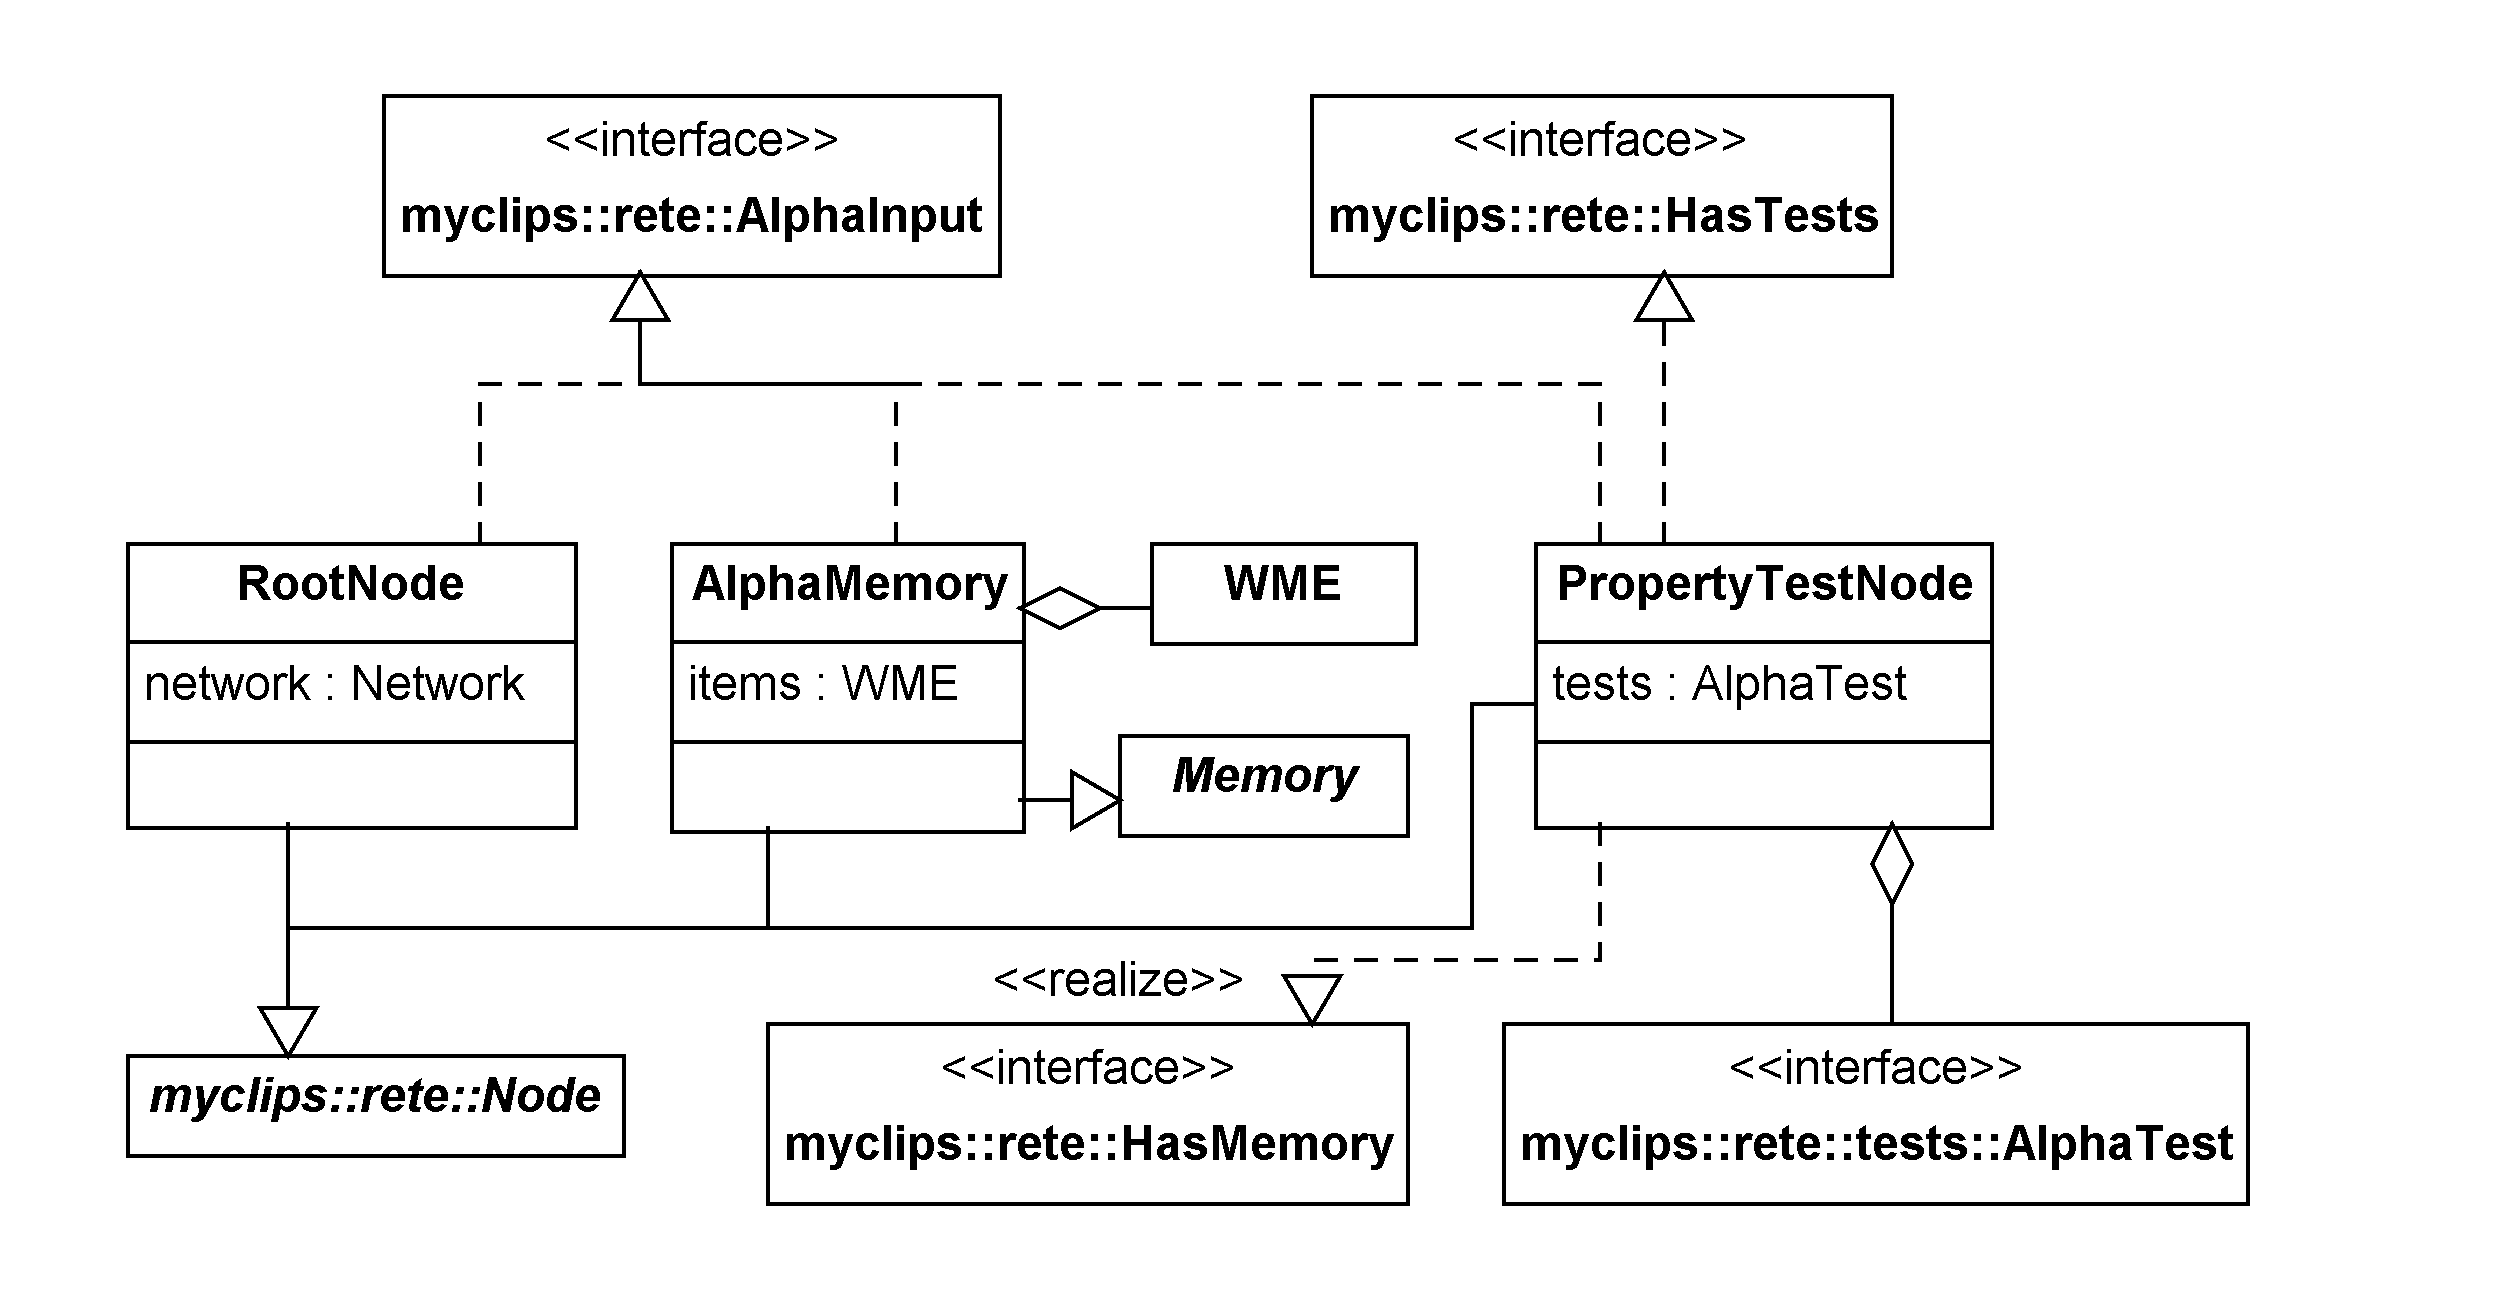
\includegraphics[width=1\textwidth]{Immagini/Capitolo3/Classi/myclips_rete_nodes_Nodi-Alpha.png}
\caption{Package \emph{myclips.rete.nodes}: vista dei nodi della pozione \emph{alpha}}\label{fig:class-myclips-rete-nodes-alpha}
\end{figure}

\begin{figure}
\centering
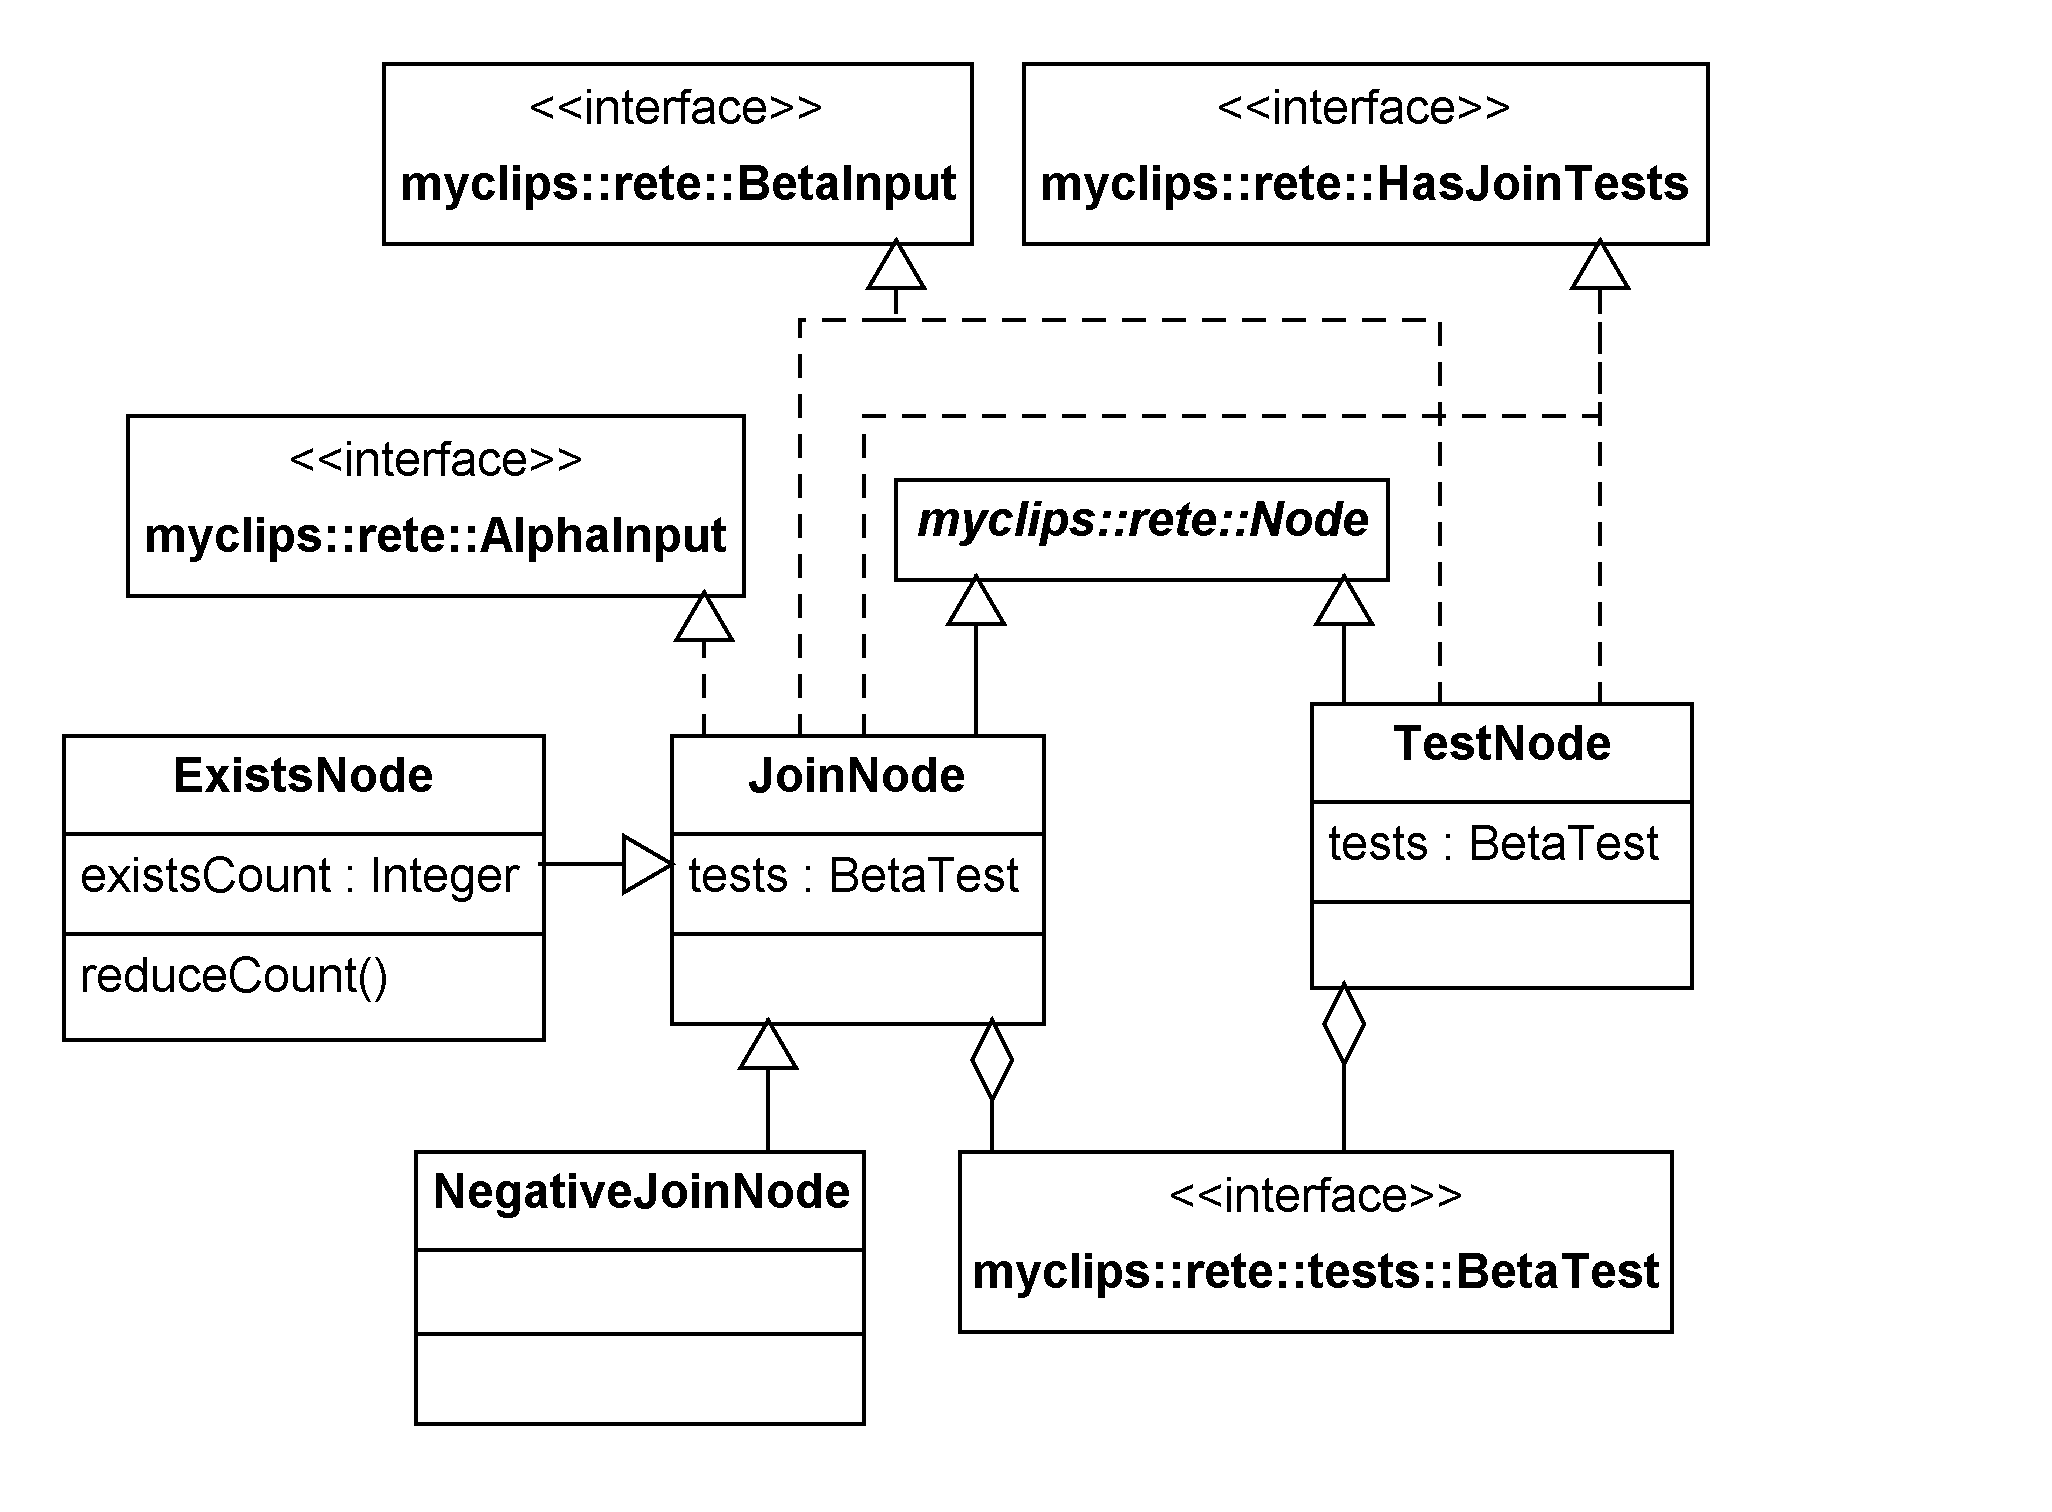
\includegraphics[width=1\textwidth]{Immagini/Capitolo3/Classi/myclips_rete_nodes_Join-Tests-Exists-Negative-Nodes.png}
\caption{Package \emph{myclips.rete.nodes}: vista dei nodi della pozione \emph{beta}}\label{fig:class-myclips-rete-nodes-beta}
\end{figure}

\begin{figure}
\centering
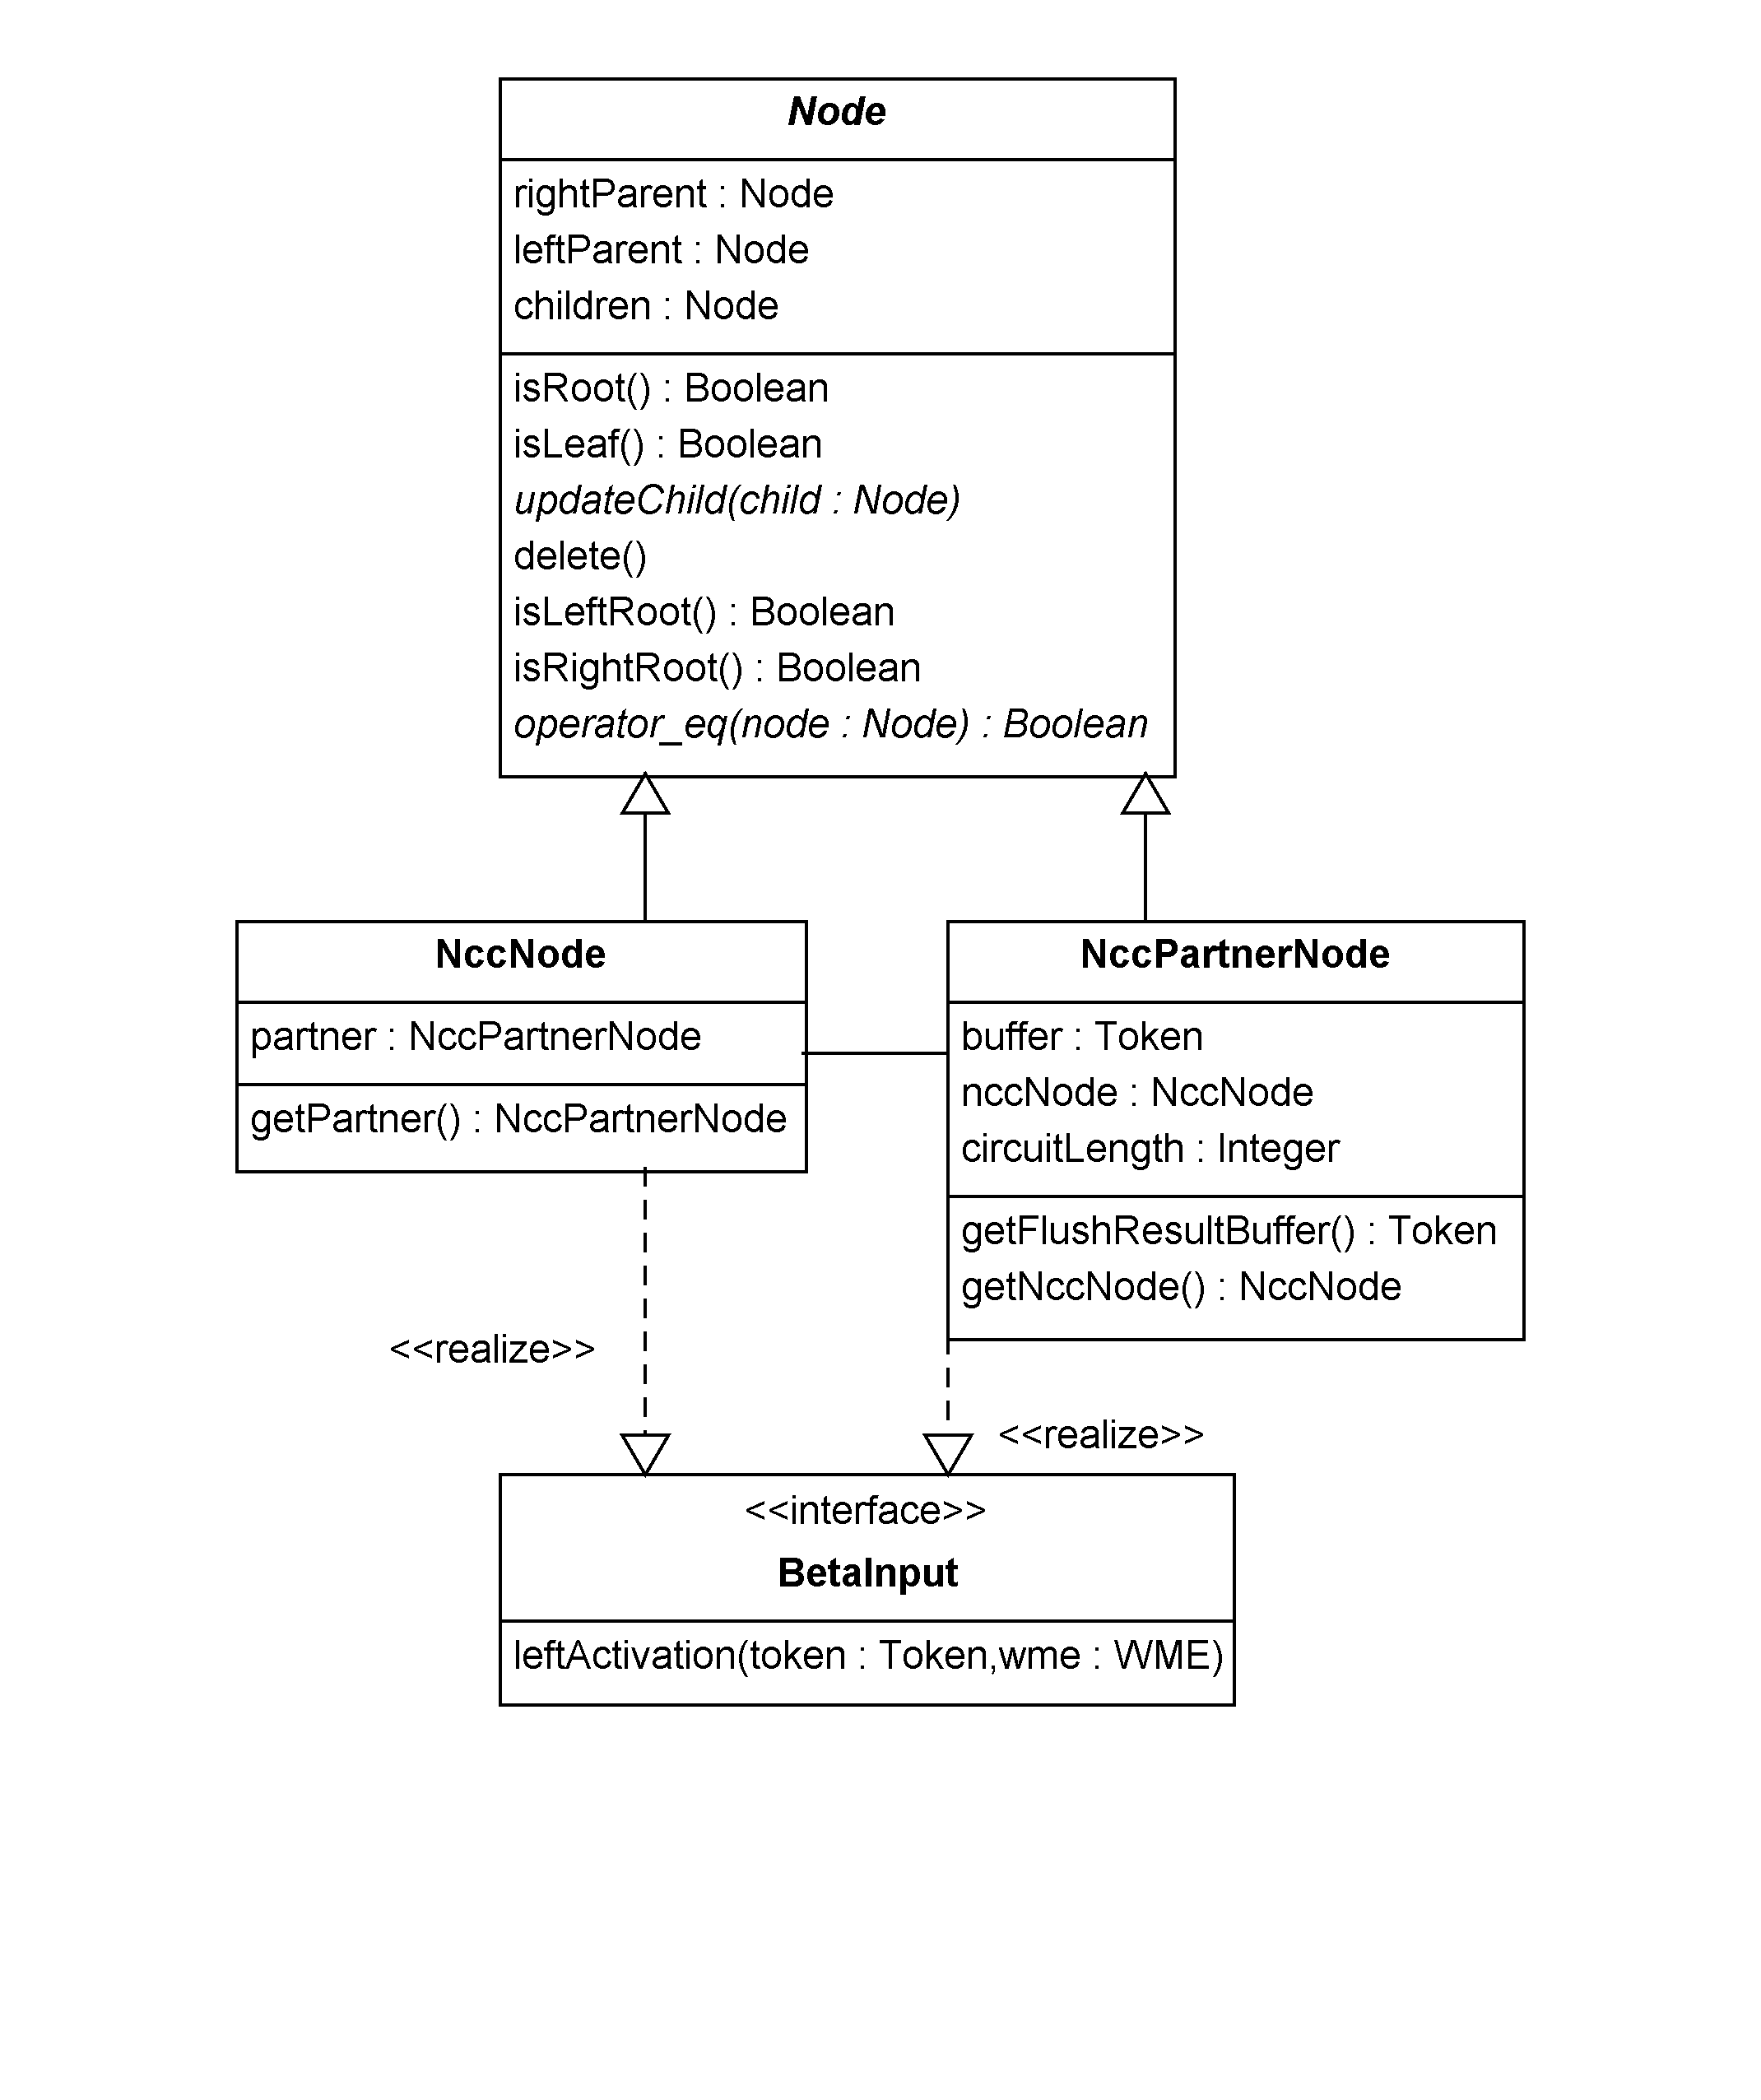
\includegraphics[width=1\textwidth]{Immagini/Capitolo3/Classi/myclips_rete_nodes_Ncc-Partner-Nodes.png}
\caption{Package \emph{myclips.rete.nodes}: vista dei nodi della pozione \emph{beta} (nodi \emph{Ncc})}\label{fig:class-myclips-rete-nodes-beta-ncc}
\end{figure}


Una classificazione approssimativa dei nodi può essere realizzata suddividendoli in base alla porzione della RETE che realizzano: \emph{alpha}~(\figurename~\ref{fig:class-myclips-rete-nodes-alpha}) o \emph{beta}~(\figurename~\ref{fig:class-myclips-rete-nodes-beta} e \ref{fig:class-myclips-rete-nodes-beta-ncc}). 

Ogni tipo di nodo svolge una specifica funzione, spesso anche in relazione alla tipologia di test che può inglobare:
\begin{description}
	\item[RootNode:] la radice del grafo radicato orientato che realizza RETE.
	
	\item[PropertyTestNode:] associabile a test di tipo \emph{alpha}, può effettuare controlli su elementi costanti di un pattern.
	
	\item[AlphaMemory:] unità locale di memoria posta a termine di ogni \emph{circuito alpha}. Conserva gli elementi \emph{WME} che hanno attraversato con successo il circuito a cui il nodo è collegato.
	
	\item[JoinNode:] nodo a due input, viene utilizzato per riunire istanze \emph{WME} provenienti dai due rami del grafo in \emph{Token} da propagare se i test collegati al nodo risultano verificati. Questo tipo di nodi viene utilizzato per realizzare i test di coerenza sul valore delle variabili presenti in pattern multipli.
	
	\item[NegativeJoinNode:] specializzazione del nodo \emph{JoinNode}, propaga un \emph{Token} solo se tutti i test di coerenza associati al nodo non risultano soddisfatti.
	
	\item[TestNode:] nodo con input singolo, esegue dei test su un \emph{Token} (spesso associati all'esecuzioni di funzioni dinamiche) e lo propaga nei casi di esito positivo.

	\item[ExistsNode:] nodo a due input utilizzato per fornire supporto al quantificatore esistenziale ($\exists$) all'interno delle porzioni LHS delle regole. Un'attivazione proveniente dal ramo sinistro (quindi \emph{beta}) del grafo viene propagato soltanto se esiste almeno un elemento all'interno dell'unità di memoria collegata come input destro (quindi \emph{alpha}).
	
	\item[NccNode] e \textbf{NccPartnerNode:} i nodi \emph{Ncc}~(\figurename~\ref{fig:class-myclips-rete-nodes-beta-ncc}) vengono utilizzati per realizzare negazioni di gruppi di condizioni. Le attivazioni provenienti dal ramo sinistro vengono propagate soltanto quando non viene identificata nessuna attivazione proveniente dal circuito negato associato.
	
\end{description} 

\paragraph{Classi di Test}

Gli algoritmi utilizzati dai nodi per eseguire le verifiche sulle attivazioni e gli elementi della \emph{working-memory} sono organizzati all'interno del \emph{package} \emph{myclips.rete.tests}. Alla base della strategia di progettazione dei test c'è l'utilizzo del \emph{design pattern} comportamentale \emph{Strategy}: allo scopo di rendere gli algoritmi di test intercambiabili fra loro, vengono fornite due interfacce di base che tutti i test realizzano. La scelta dell'interfaccia da implementare indica la classe di nodi che potranno utilizzare i test: \emph{AlphaTest} per i test utilizzabili nei nodi \emph{Alpha}, \emph{BetaTest} per quelli nei nodi \emph{Beta}.

\begin{figure}
\centering
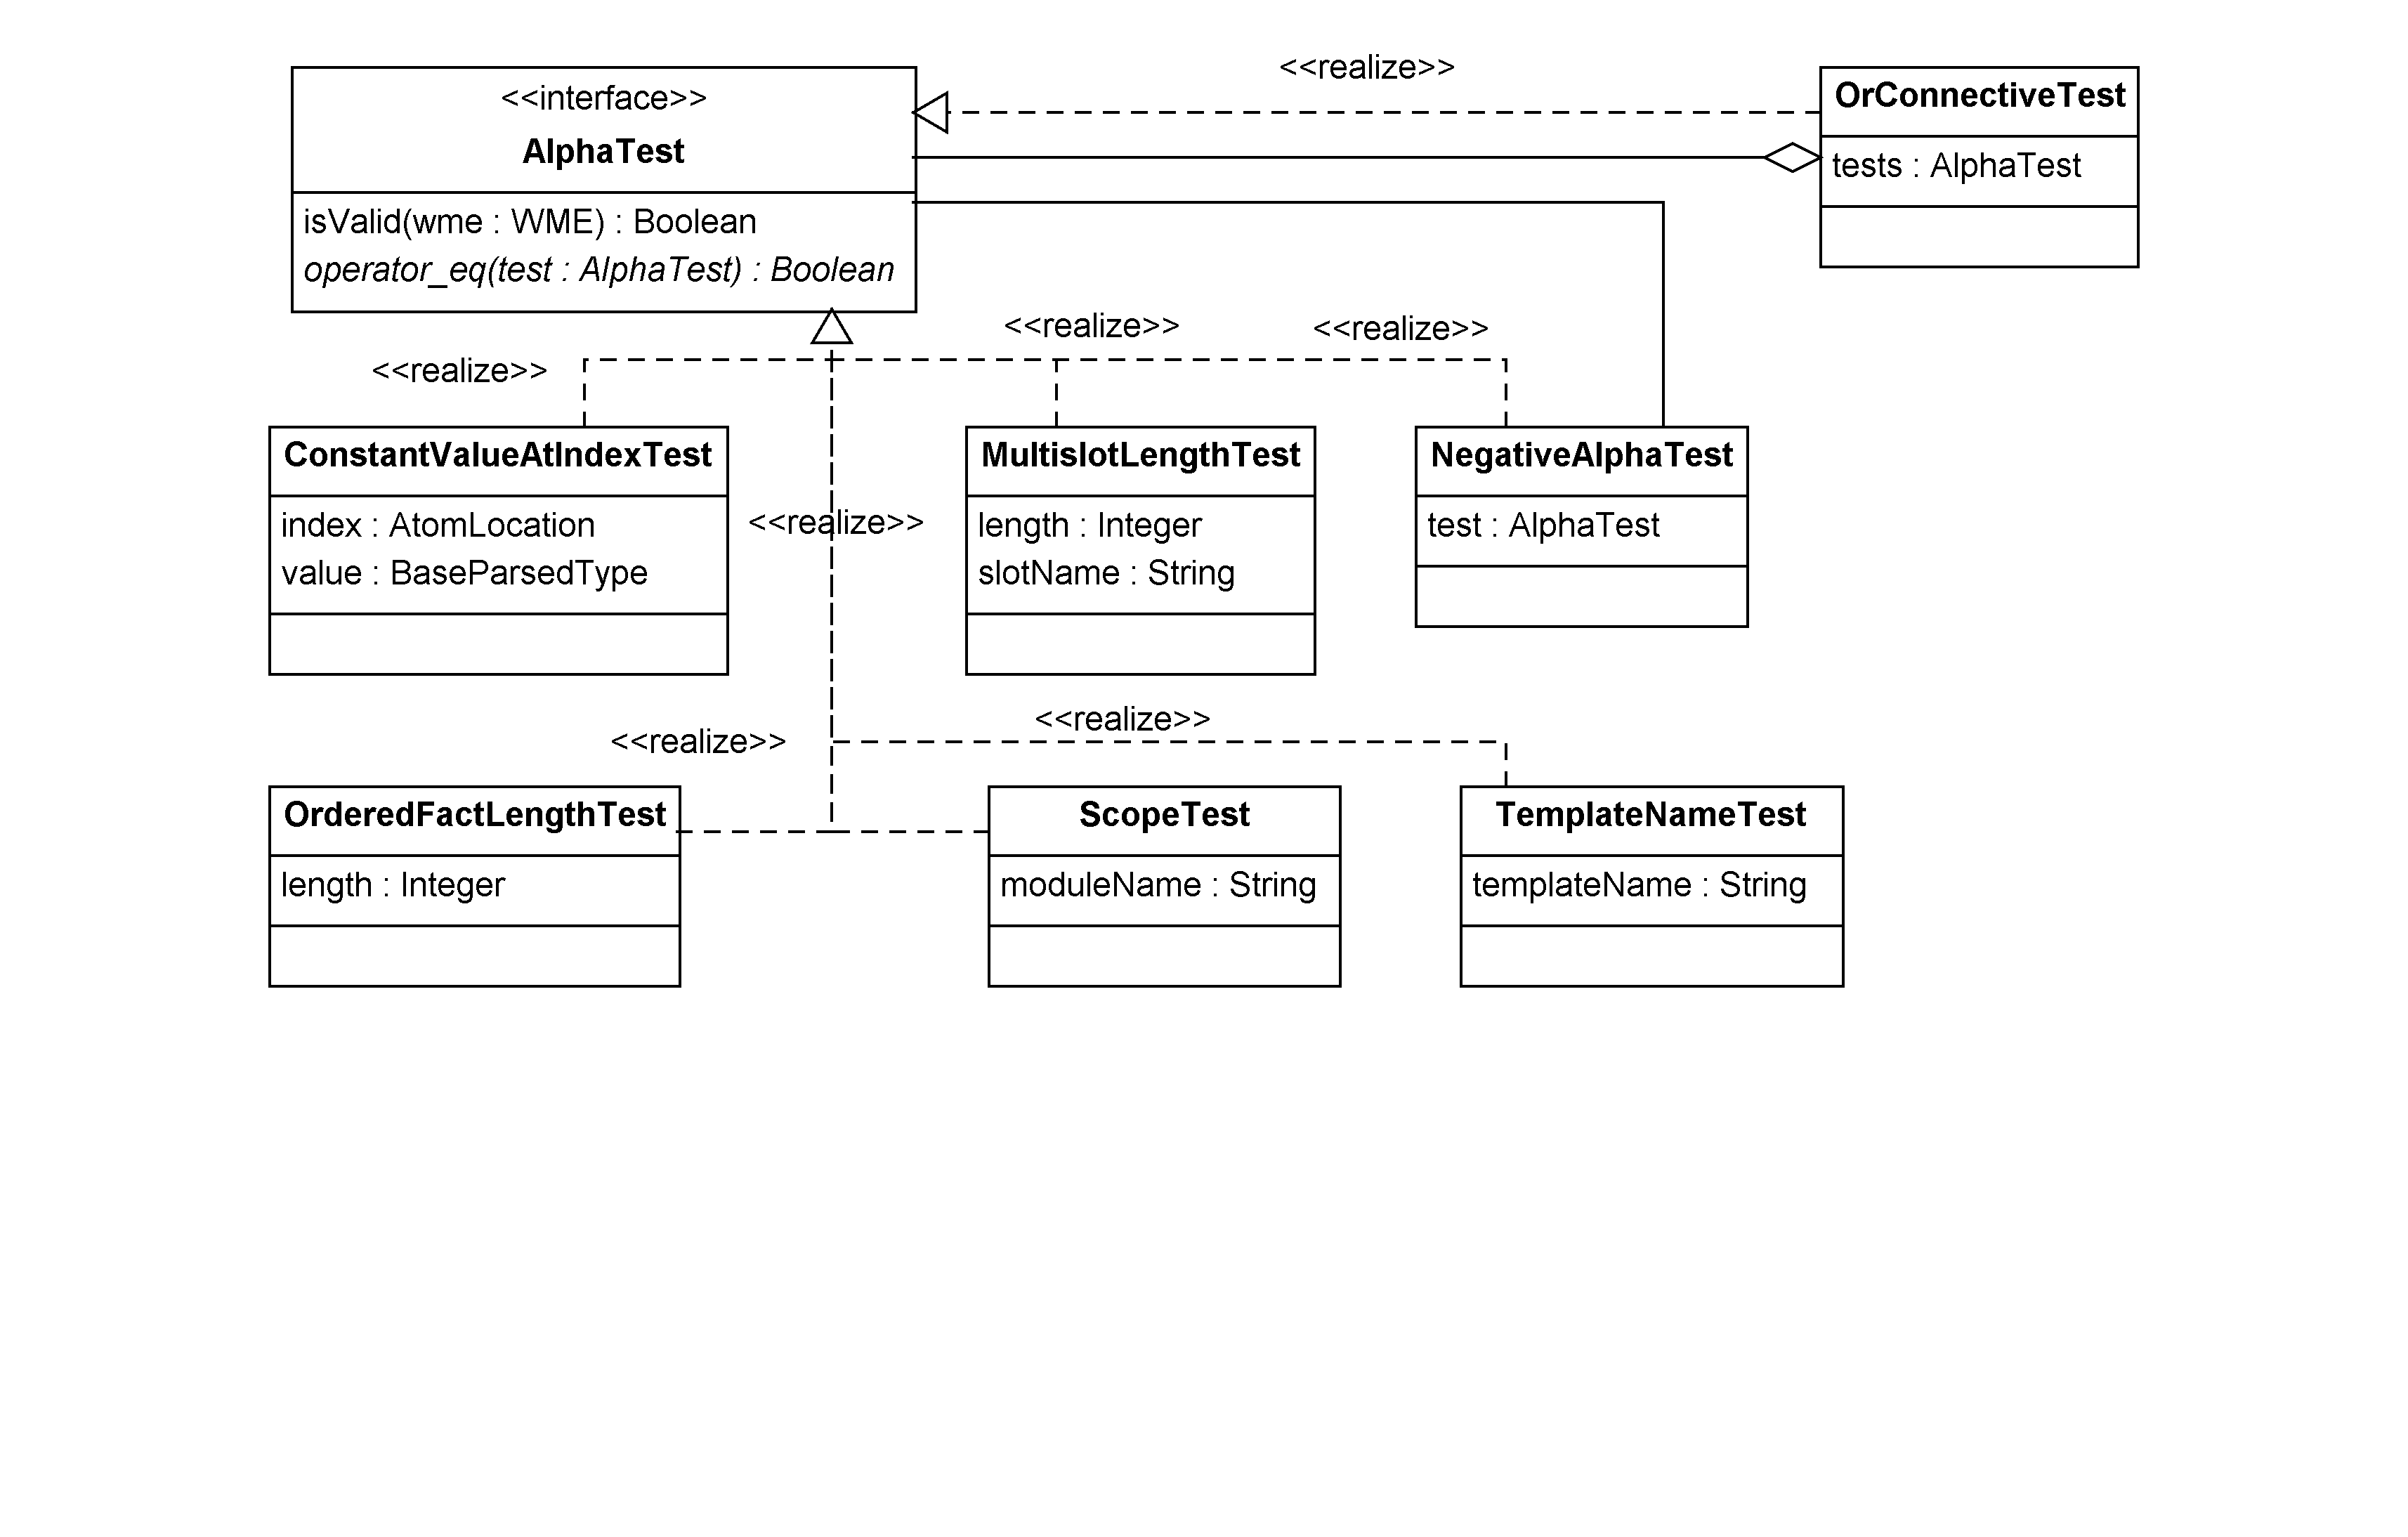
\includegraphics[width=1\textwidth]{Immagini/Capitolo3/Classi/myclips_rete_tests_Alpha.png}
\caption{Package \emph{myclips.rete.tests}: vista dei test eseguiti nella porzione \emph{alpha}}\label{fig:class-myclips-rete-tests-alpha}
\end{figure}

La prima tipologia (\figurename~\ref{fig:class-myclips-rete-tests-alpha}) esegue test su singoli elementi \emph{WME}, valutando il possibile inserimento all'interno delle memorie locali presenti al termine dei circuiti \emph{alpha}. Gli algoritmi possono valutare caratteristiche differenti dei singoli elementi come la lunghezza delle sequenze di \emph{OrderedFact}, la visibilità relativa ad un determinato \emph{Scope}, la presenza di un elemento costante in una determinata coordinata, etc.

\begin{figure}[h]
\centering
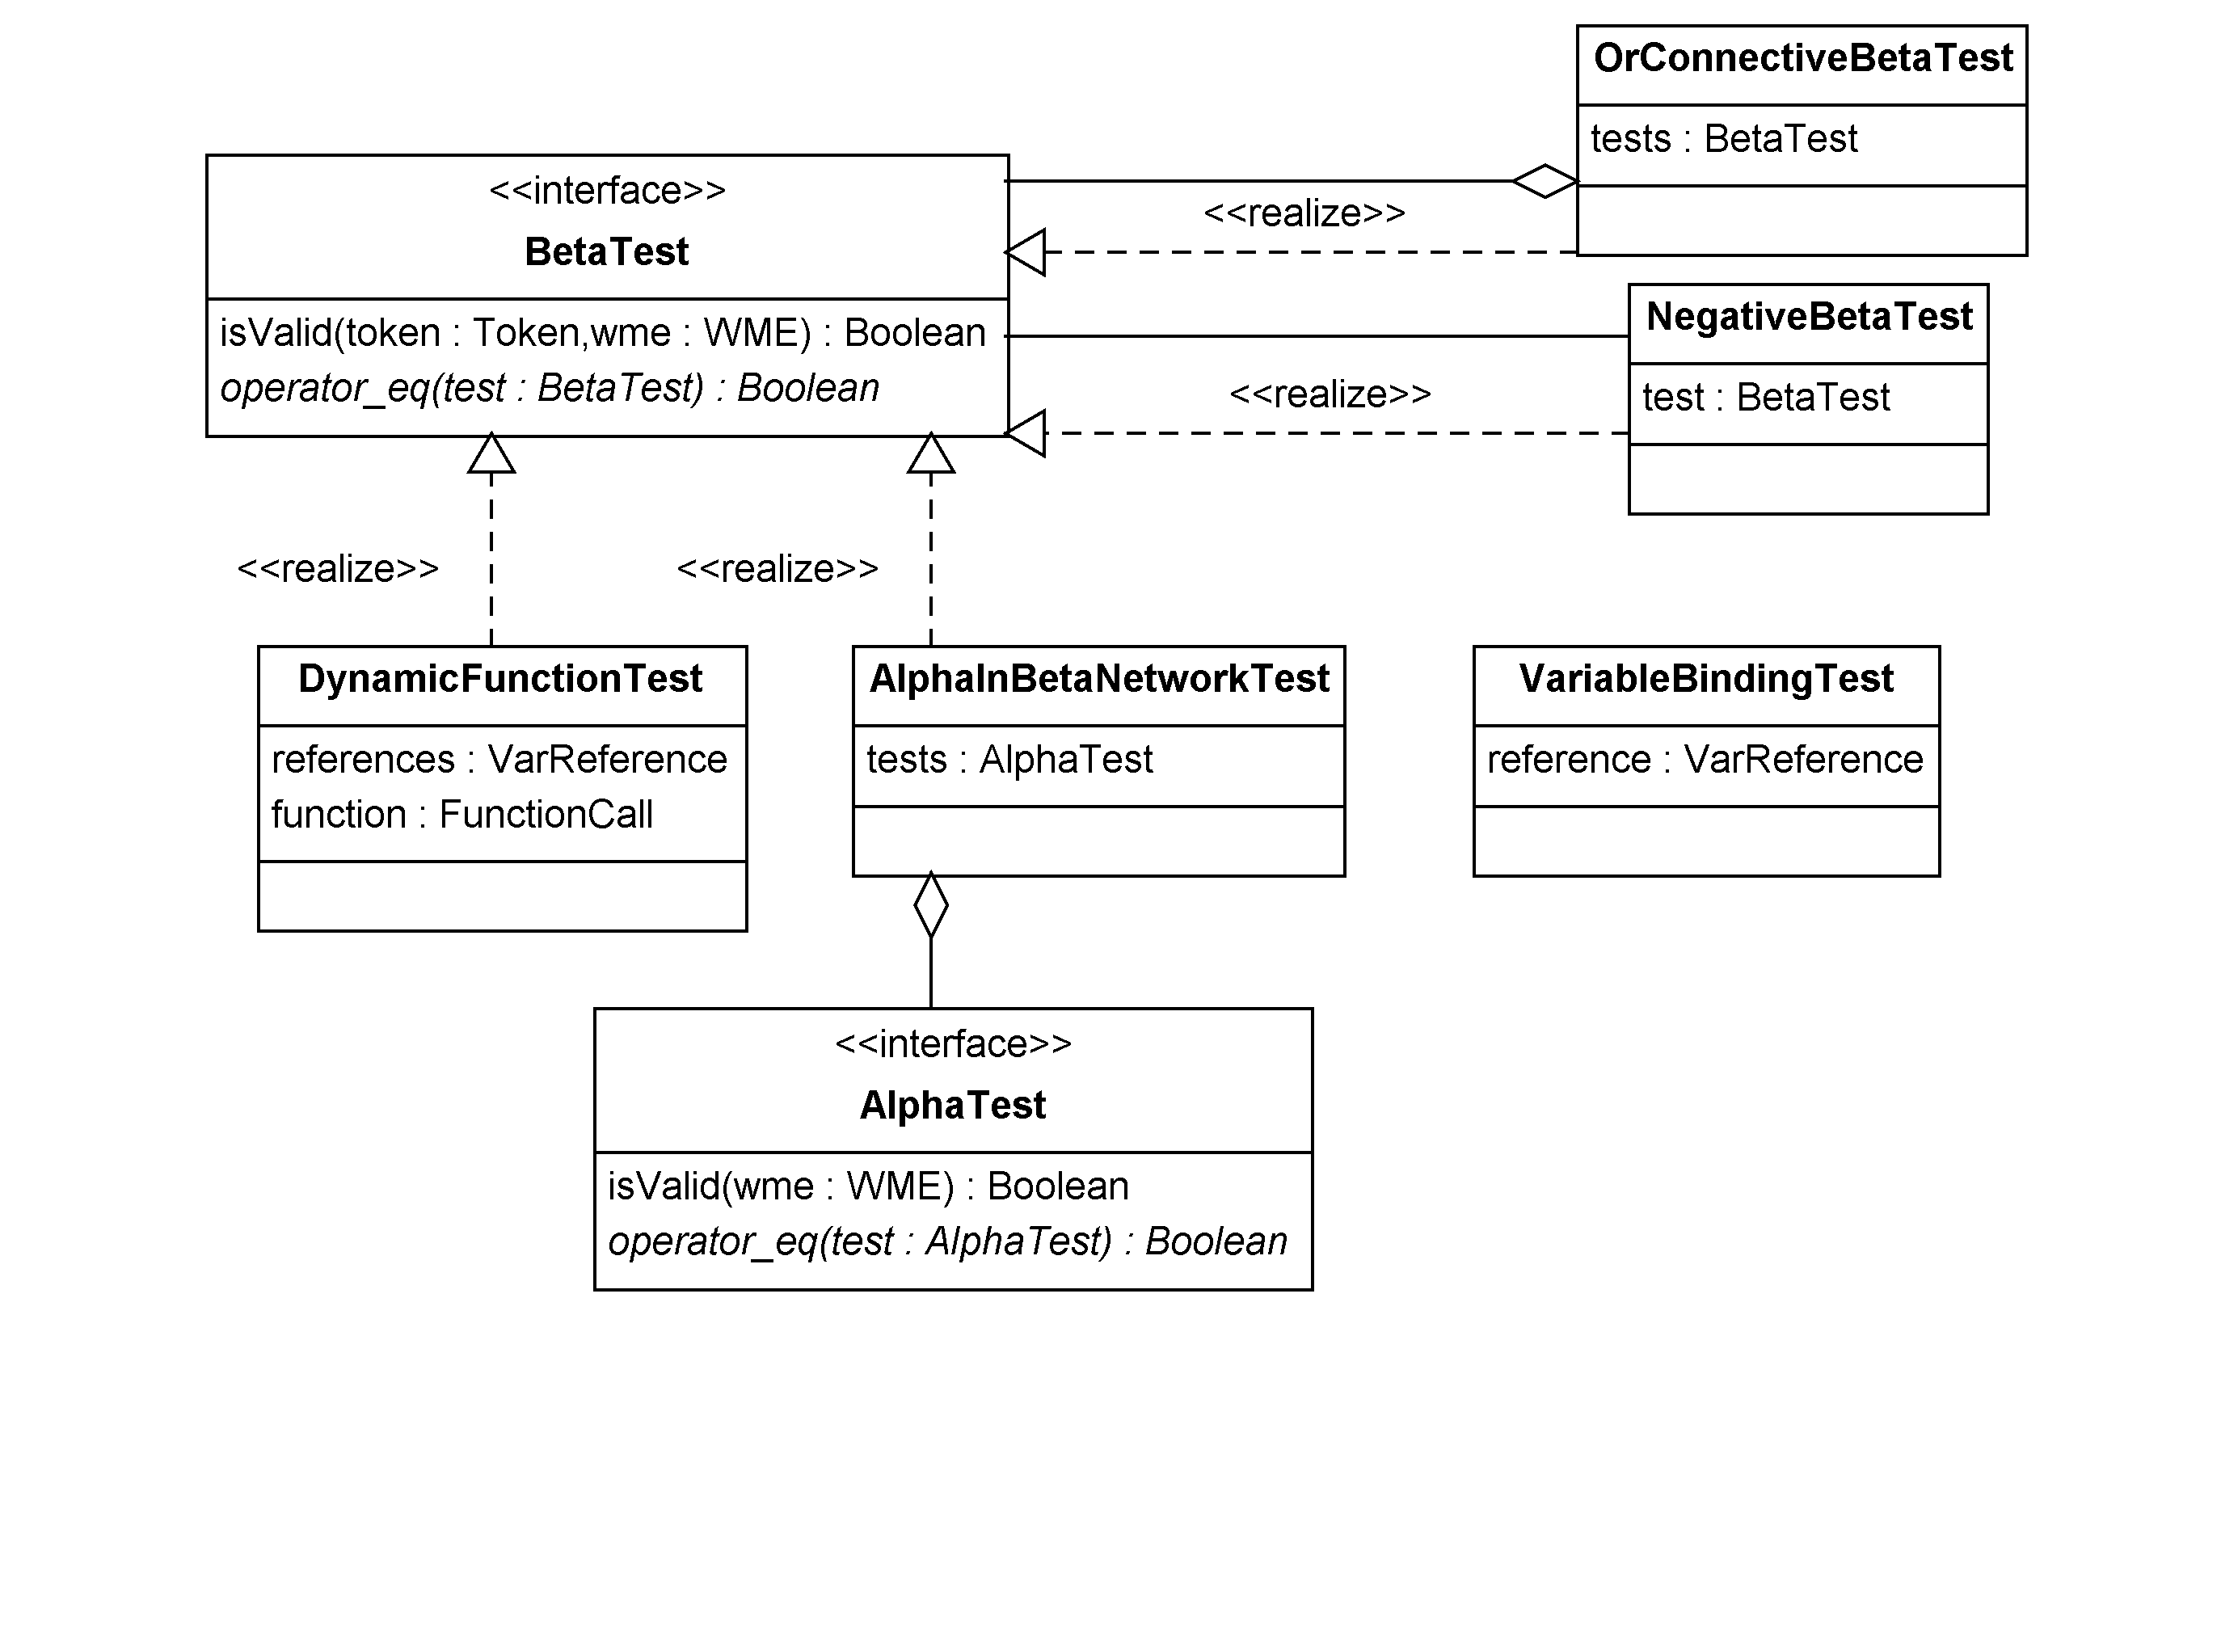
\includegraphics[width=1\textwidth]{Immagini/Capitolo3/Classi/myclips_rete_tests_Beta.png}
\caption{Package \emph{myclips.rete.tests}: vista dei test eseguiti nella porzione \emph{beta}}\label{fig:class-myclips-rete-tests-beta}
\end{figure}

La seconda tipologia (\figurename~\ref{fig:class-myclips-rete-tests-beta}) esegue verifiche su gruppi di \emph{WME}, rappresentati da \emph{Token}, valutando la coerenza del valore di variabili comuni a più pattern, il risultato dell'esecuzione di funzioni o valutando i risultato di test di tipo \emph{alpha} eseguiti nella porzione \emph{beta} del grafo. Al fine di poter eseguire i test di tipo \emph{alpha} nei nodi di tipo \emph{beta} è stata adottata una strategia facente riferimento al \emph{design pattern} strutturale \emph{Adapter} (anche noto con il nome di \emph{Wrapper} o \emph{Translator}): la classe \emph{AlphaInBetaNetworkTest}, che realizza l'interfaccia \emph{BetaTest}, incapsula oggetti con interfaccia \emph{AlphaTest} al suo interno. Le operazioni di traduzione degli argomenti dei test vengono eseguite all'interno dell'implementazione della classe.

\subsubsection{Modulo Interprete}

\begin{figure}[h]
\centering
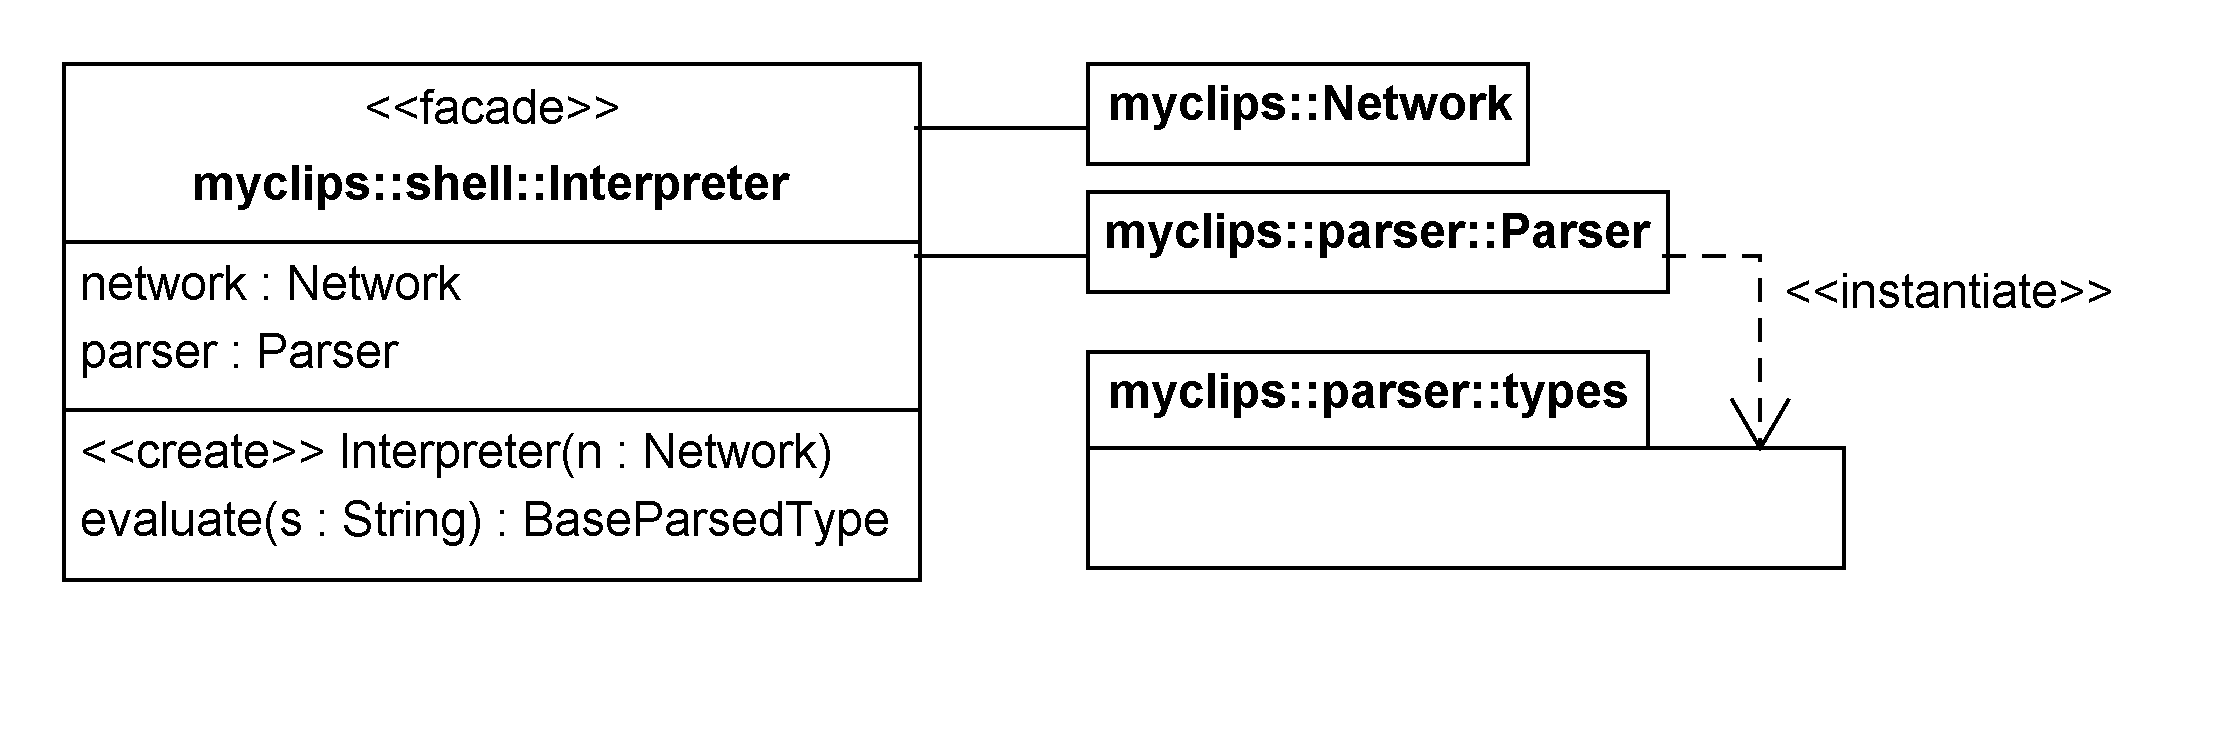
\includegraphics[width=1\textwidth]{Immagini/Capitolo3/Classi/myclips_shell_Interpreter.png}
\caption{Package \emph{myclips.rete.shell}: vista della classe \emph{Interpreter}}\label{fig:class-myclips-shell-interpreter}
\end{figure}

Il modulo \emph{Interprete}, contenuto nel \emph{package} \emph{myclips.shell}, consiste di un'unica classe \emph{fa\c{c}ade}: \emph{Interpreter}. Lo scopo della classe è quello semplificare ed unificare le operazioni di \emph{parsing} e valutazione dei costrutti, associandole alle attività di inizializzazione del \emph{motore inferenziale} e all'esecuzione del ciclo principale~(\figurename~\ref{fig:class-myclips-shell-interpreter}).

L'unica attività svolta dall'\emph{Interpreter} è quella di inizializzare un'istanza del \emph{Parser}, richiedere la valutazione di stringhe rappresentanti singoli \emph{costrutti} o \emph{comandi} e, se necessario, avviare l'interpretazione del costrutto dal parte di un'istanza di \emph{Network}. Nel caso l'elemento valutato dal parser sia un \emph{comando} (una chiamata a funzione di sistema), l'interprete provvede all'esecuzione dello stesso.

\subsubsection{Modulo Events Manager}

\begin{figure}[h]
\centering
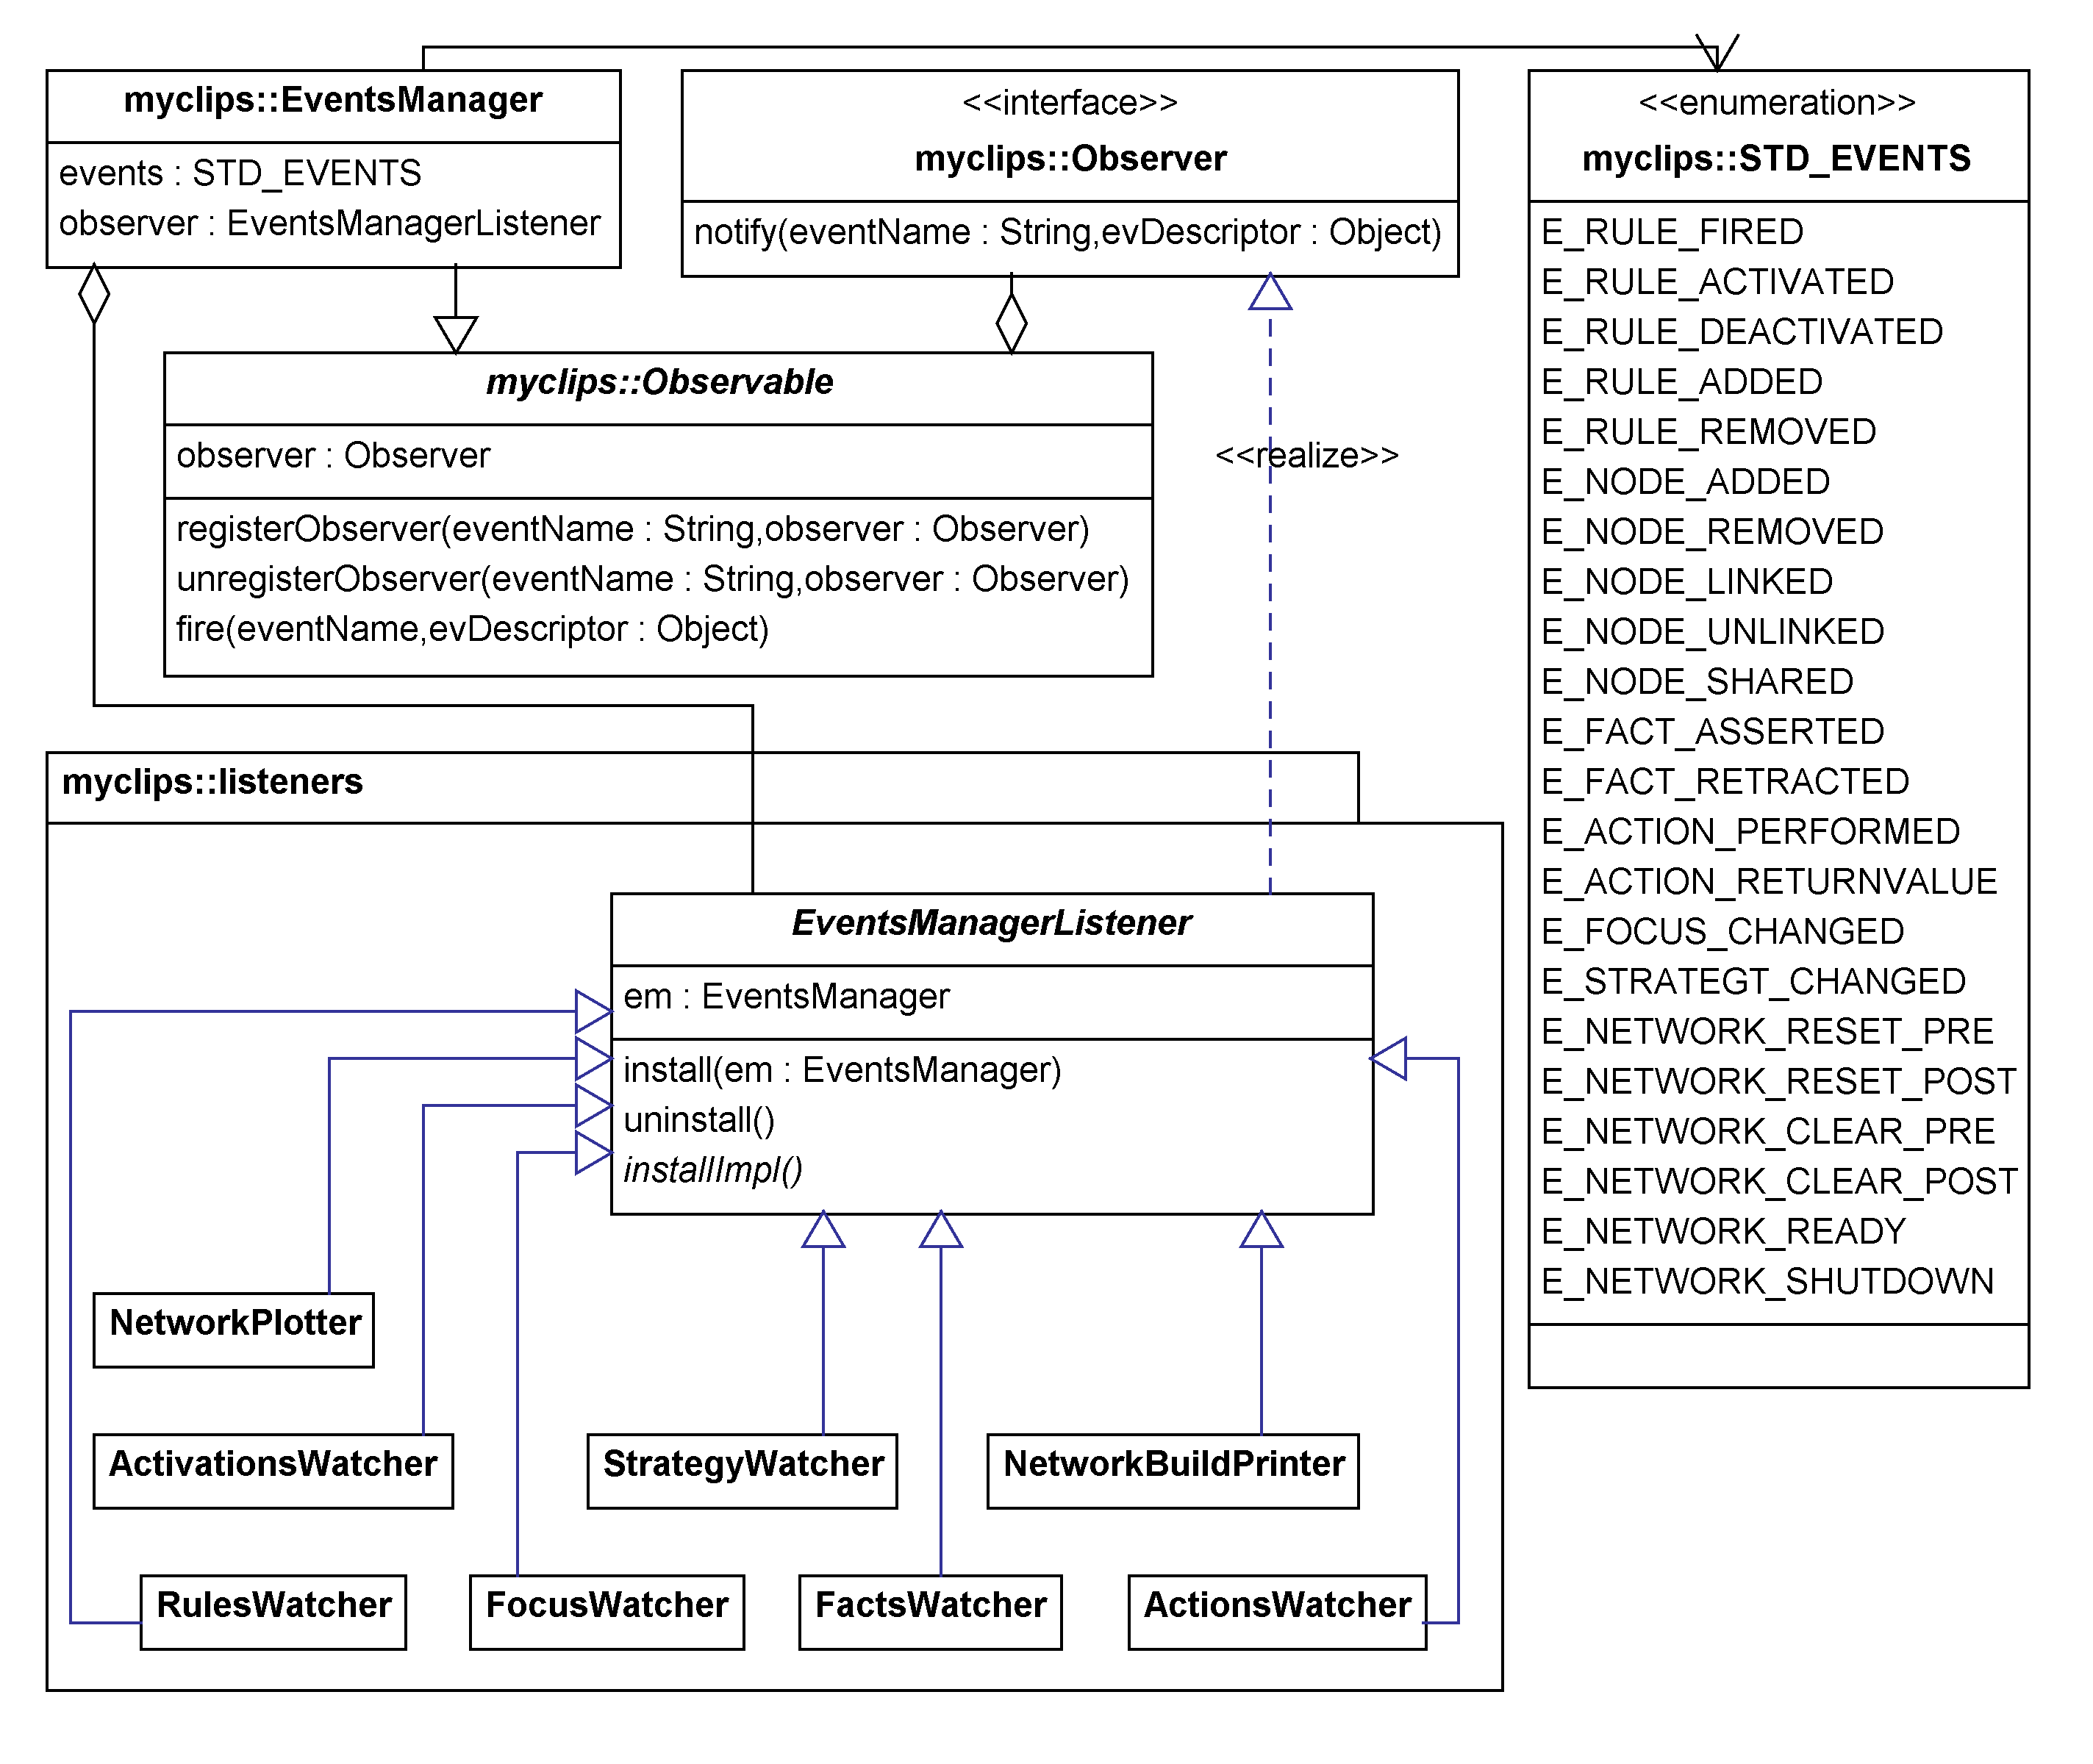
\includegraphics[width=1\textwidth]{Immagini/Capitolo3/Classi/myclips_EventsManager-Listeners.png}
\caption{Package \emph{myclips.rete.listeners}: vista della classi per la gestione degli eventi}\label{fig:class-myclips-eventsmanager}
\end{figure}

La gestione degli eventi è affidata alla collaborazione fra la classe \emph{EventsManager}, posta nel \emph{package} \emph{myclips}, e i \emph{listeners} riuniti nel \emph{package} \emph{myclips.listeners}~(\figurename~\ref{fig:class-myclips-eventsmanager}).

Usando come base l'infrastruttura offerta dallo schema \emph{Observer/Observable}, la classe \emph{EventsManager} viene utilizzata nel sistema per notificare il verificarsi di eventi. In aggiunta ad una serie di eventi predefiniti raggruppati in \emph{STD\_EVENTS}, la classe consente di notificare un qualsiasi evento personalizzato all'insieme di \emph{listener} registrati.

I \emph{listener} sono classi che estendono la classe astratta \emph{EventsManagerListener}. Il sistema fornisce un gruppo di definizioni predefinite con le quali intercettare gli eventi più comuni. Ogni classe, tramite la propria implementazione, esegue un comportamento differente come risposta ai singoli eventi per i quali si registra. La procedura di registrazione dei \emph{listener} è effettuata all'interno del metodo \emph{EventsManagerListener::install}, alle super-classi viene offerta la possibilità di personalizzare la procedura tramite l'implementazione del metodo \emph{EventsManagerListener::installImpl}, realizzando in questo modo lo schema previsto dal \emph{design pattern} comportamentale \emph{Template method}.

\subsubsection{Modulo Funzioni}
Il \emph{package} \emph{myclips.functions} gestisce la collezione di funzioni di sistema, così come l'intera infrastruttura per la manipolazione della stessa~(\figurename~\ref{fig:class-myclips-functions}).

\begin{figure}
\centering
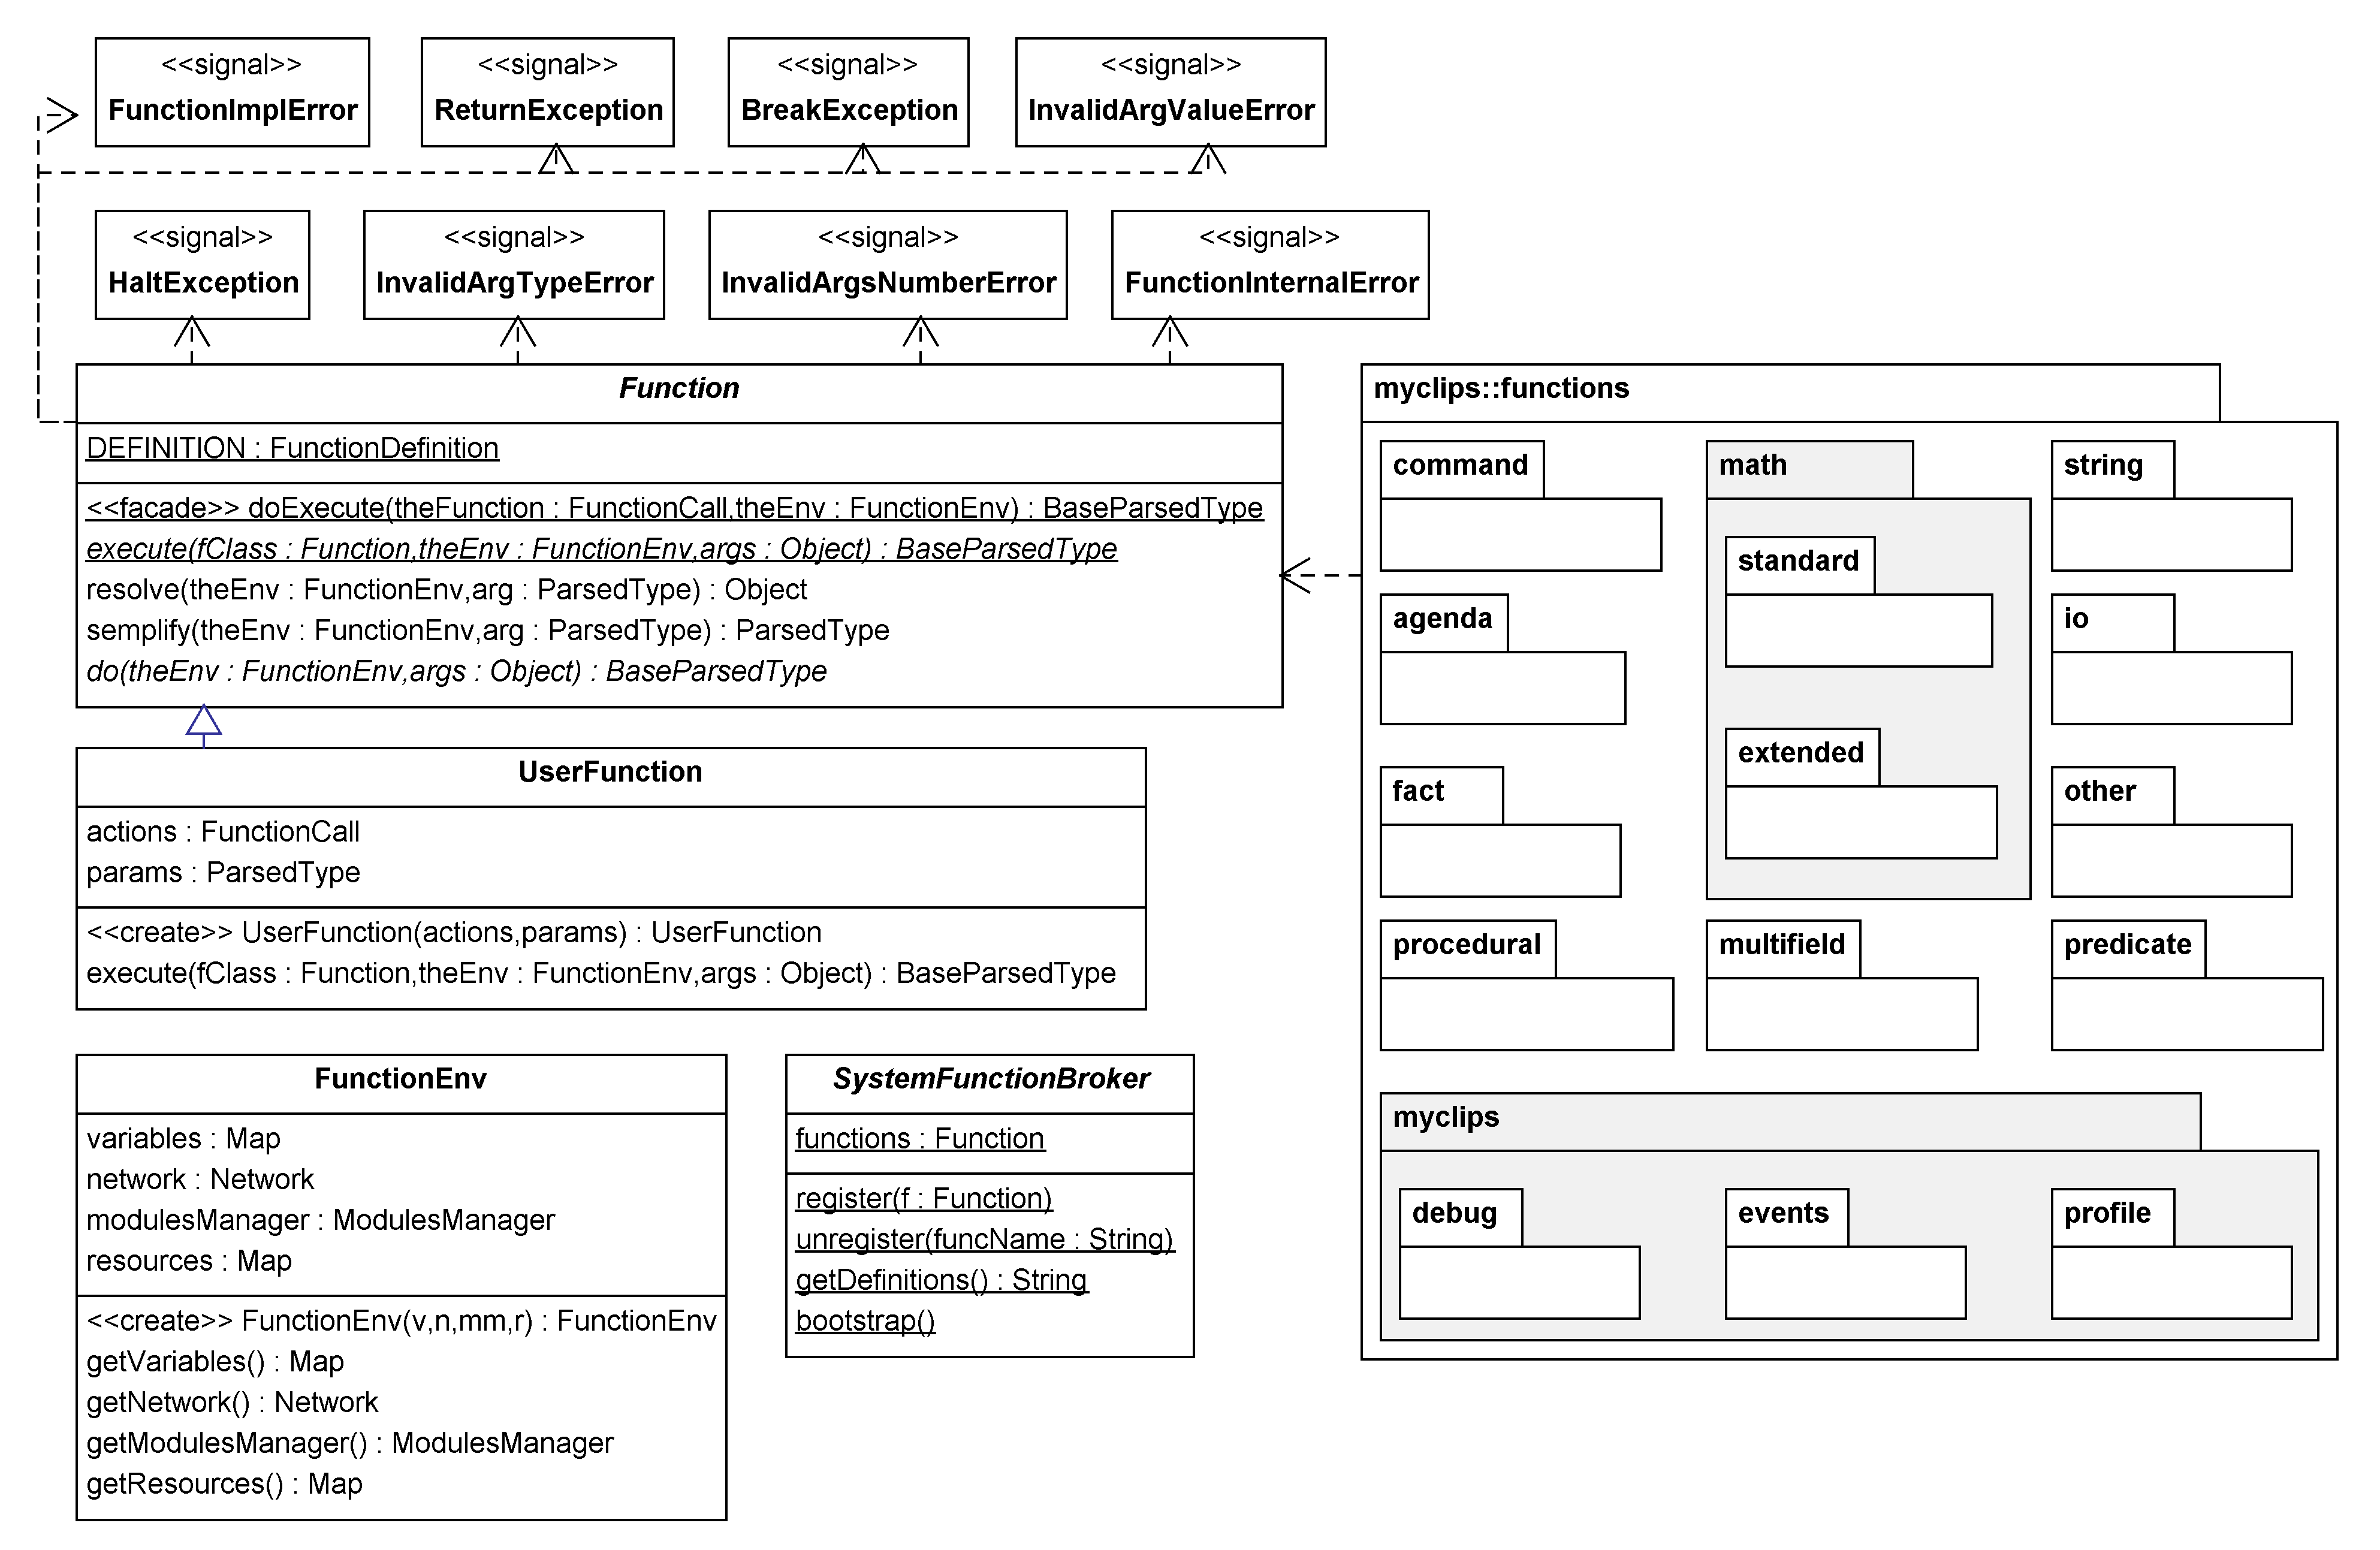
\includegraphics[width=1.3\textwidth, angle=270]{Immagini/Capitolo3/Classi/myclips_functions-Globale.png}
\caption{Package \emph{myclips.rete.functions}: vista della classi per la gestione delle funzioni di sistema}\label{fig:class-myclips-functions}
\end{figure}

Alla base di ogni funzione di sistema c'è la classe astratta \emph{Function}, la quale realizza una strategia basata sul \emph{design pattern} comportamentale \emph{Command}. Il contesto d'esecuzione delle funzioni viene fornito attraverso un'istanza di classe \emph{FunctionEnv}, la quale conserva riferimenti al \emph{Network}, \emph{ModulesManager} e alle risorse inizializzate dal sistema (l'elenco di \emph{stream di input/output}).

La base per la gestione delle definizioni è offerta dal \emph{SystemFunctionBroker}: definisce metodi per l'aggiunta o la rimozione di definizioni a \emph{run-time}, cosi come implementa il meccanismo automatico di caricamento delle definizioni partendo da un registro conservato su \emph{file} (tramite il metodo \emph{bootstrap}).

L'elenco di funzioni di sistema è distribuito all'interno del \emph{sub-package} \emph{myclips.function}. L'organizzazione adottata rispecchia la tipologia di funzioni. Le classi definite nel \emph{sub-package} \emph{myclips.functions.myclips} rappresentano funzioni originali del sistema MyCLIPS per la gestione di eventi e la valutazione degli artefatti (sia dal punto di vista prestazionale che di correttezza). Le restanti definizioni realizzano funzioni previste da CLIPS: le sintassi e le semantiche delle definizioni rispecchiano quelle previste dal software CLIPS per consentire la portabilità degli artefatti fra i sistemi.

\subsection{Server}

\begin{figure}[h]
\centering
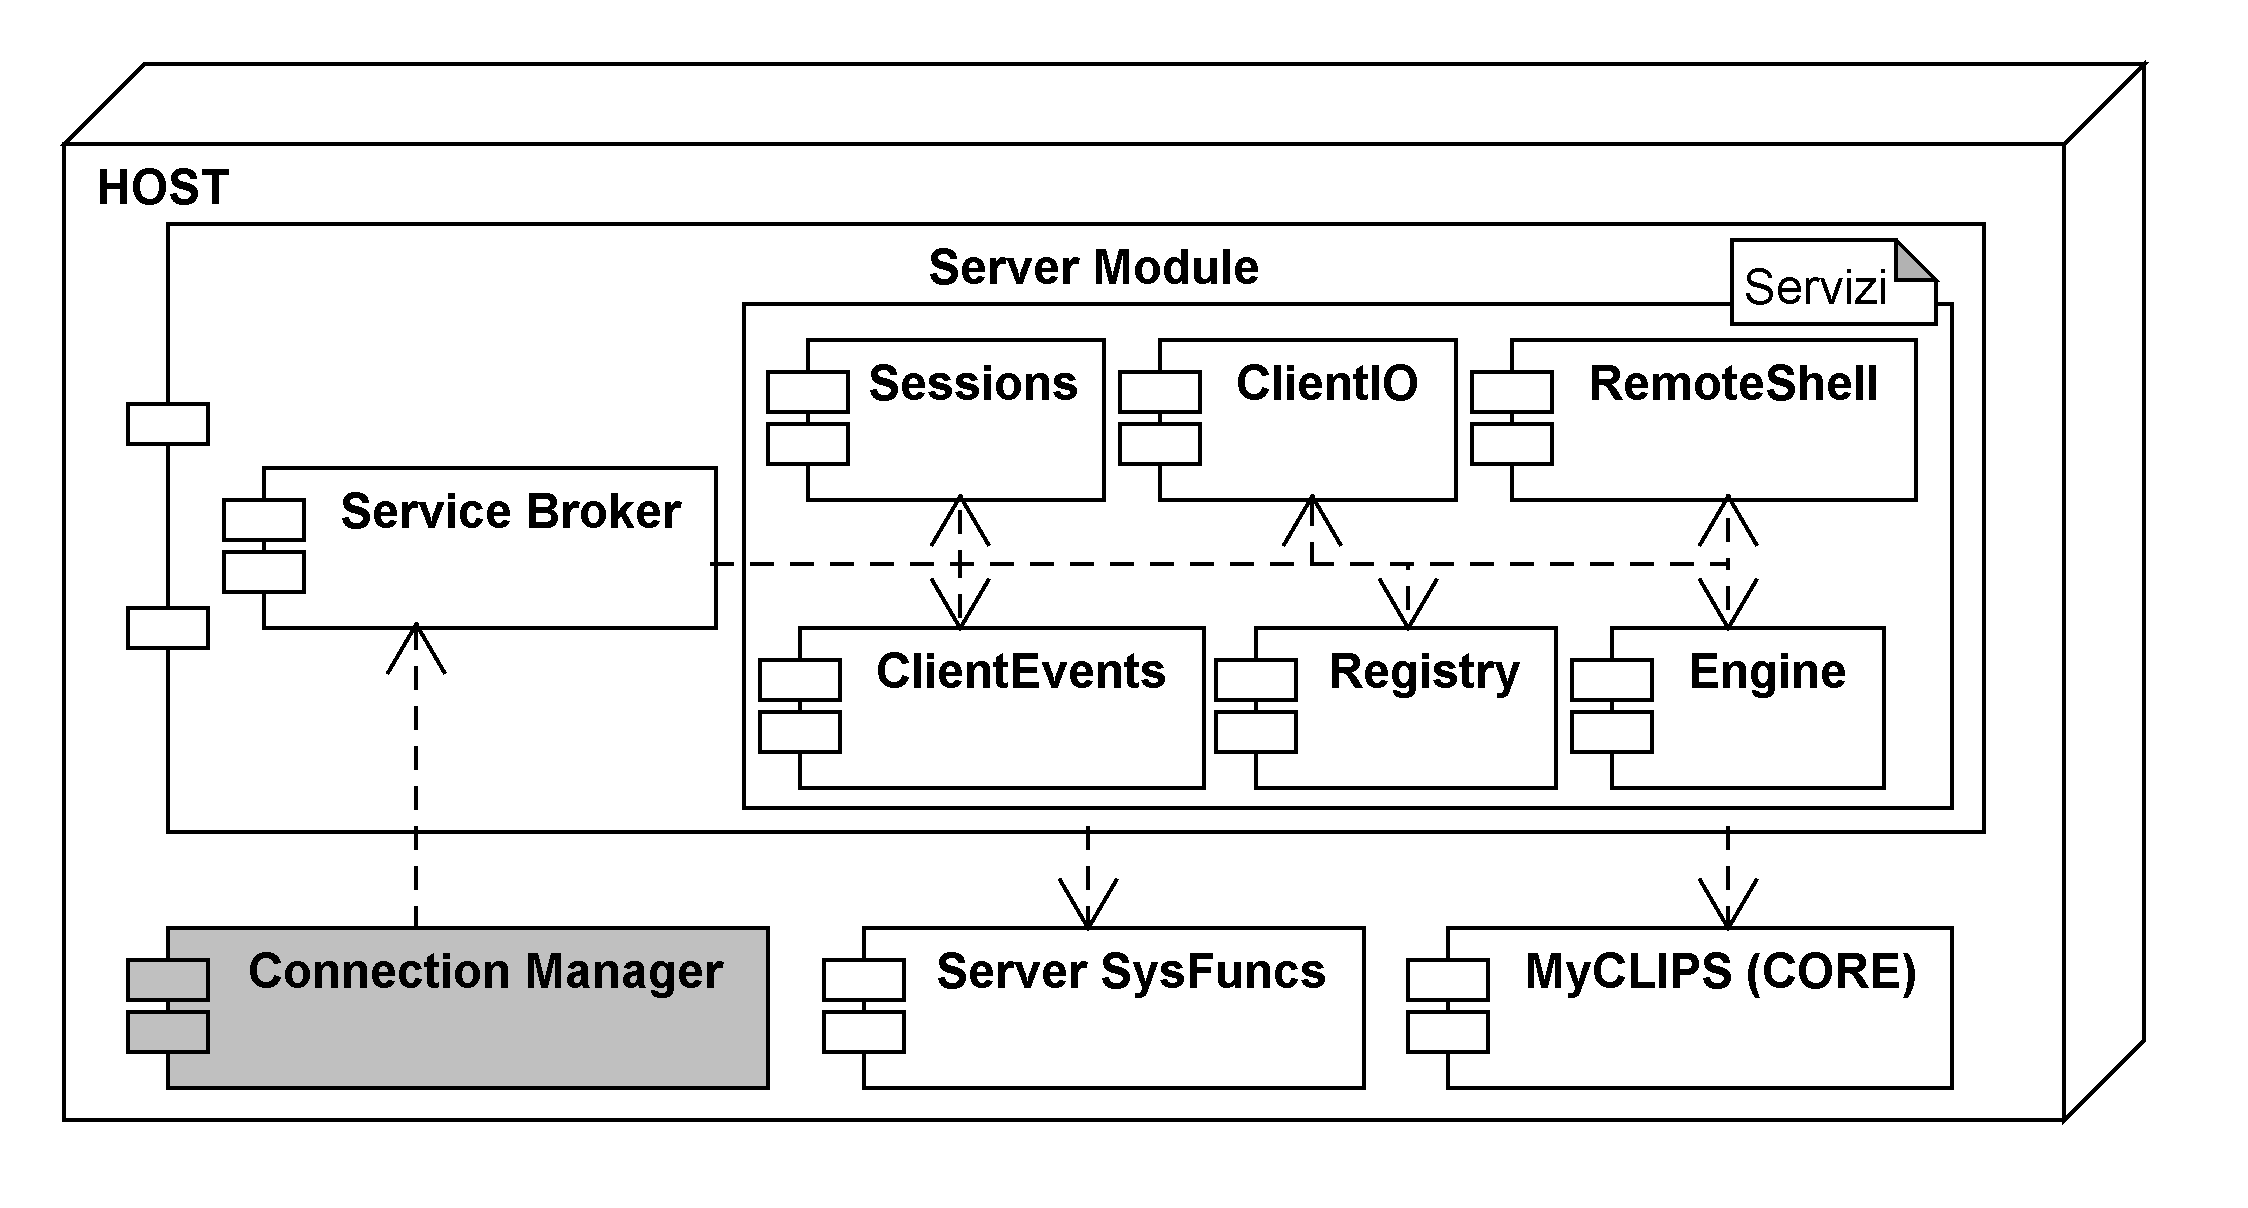
\includegraphics[width=1\textwidth]{Immagini/Capitolo3/Deployment/Server.png}
\caption{Vista generale dell'architettura server}\label{fig:architettura-server}
\end{figure}

L'architettura del modulo server rispecchia uno schema orientato alla suddivisione delle attività svolte in servizi differenti e che realizzano specifiche tipologie di interfaccia~(\figurename~\ref{fig:architettura-server}). Alla base delle implementazioni dei differenti servizi viene posto il componente software principale MyCLIPS.

\subsubsection{Broker di servizi}

\begin{figure}
\centering
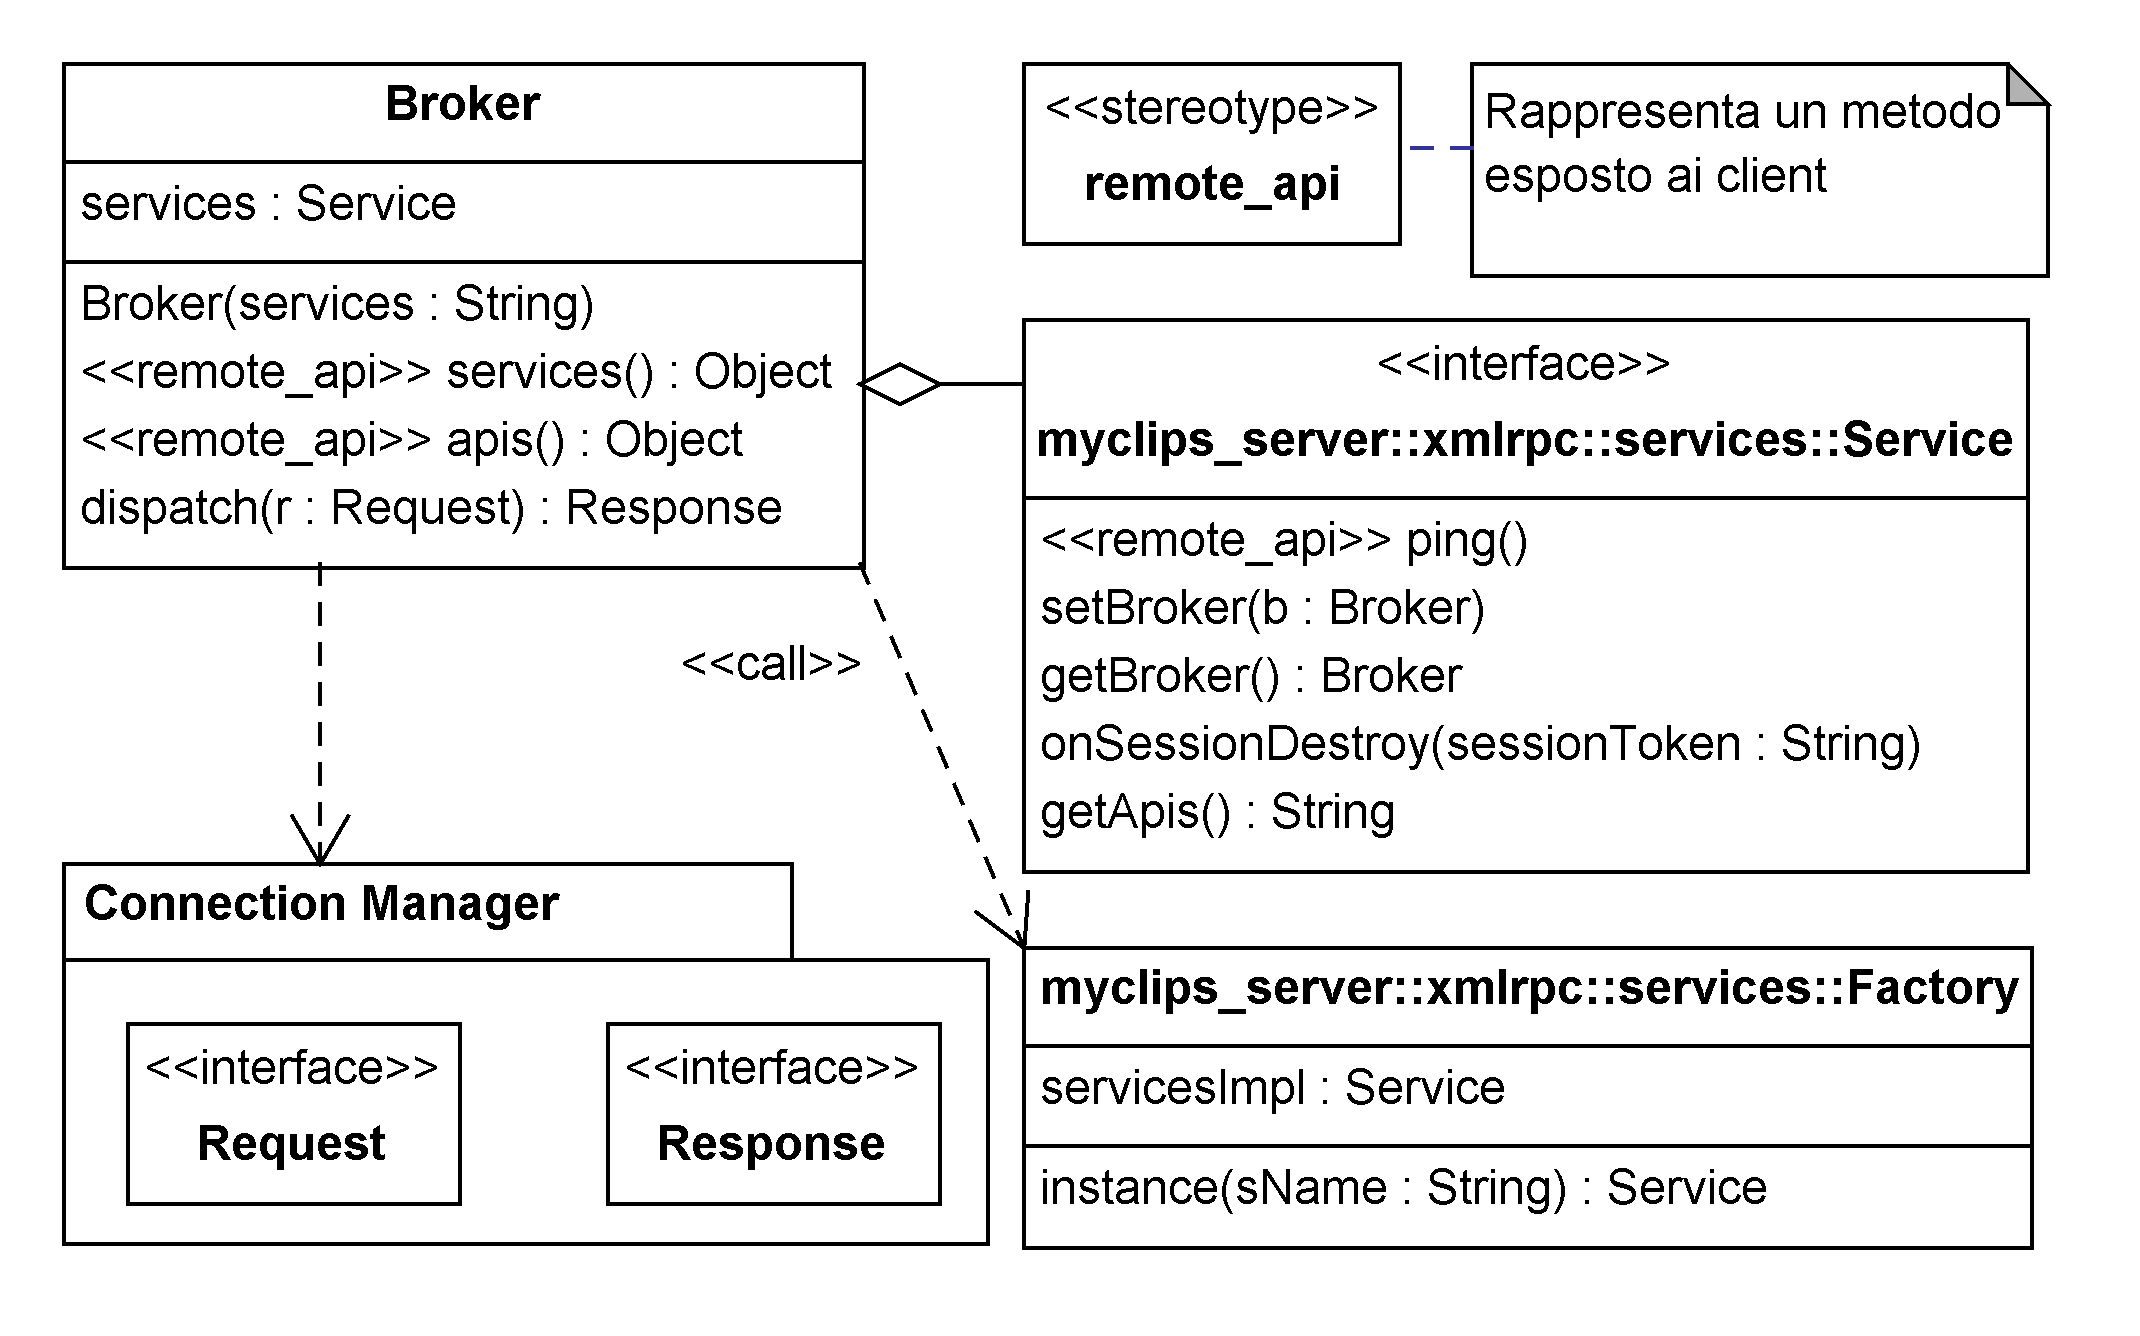
\includegraphics[width=1\textwidth]{Immagini/Capitolo3/Classi/myclips_server_Broker.png}
\caption{Package \emph{myclips\_server}: vista delle classi e interfacce relative al \emph{Broker}}\label{fig:class-myclips-server-broker}
\end{figure}

Il componente \emph{Broker}~(\figurename~\ref{fig:class-myclips-server-broker}) ha il compito di organizzare i servizi offerti dal modulo \emph{server}, controllando il flusso di richieste e risposte provenienti dall'infrastruttura addetta alla gestione delle connessioni con i client.

La realizzazione dell'interfaccia \emph{Service}, richiesta ad ogni classe concreta di servizio, garantisce l'implementazione dei metodi necessari alla registrazione della classe nel \emph{Broker}. L'interfaccia viene ulteriormente estesa da ogni tipologia specifica di servizio.

La creazione delle istanze concrete dei servizi viene delegata alle funzioni del \emph{Service Factory} (classe \emph{Factory} in \figurename~\ref{fig:class-myclips-server-broker})

\subsubsection{Servizio Sessioni}

\begin{figure}
\centering
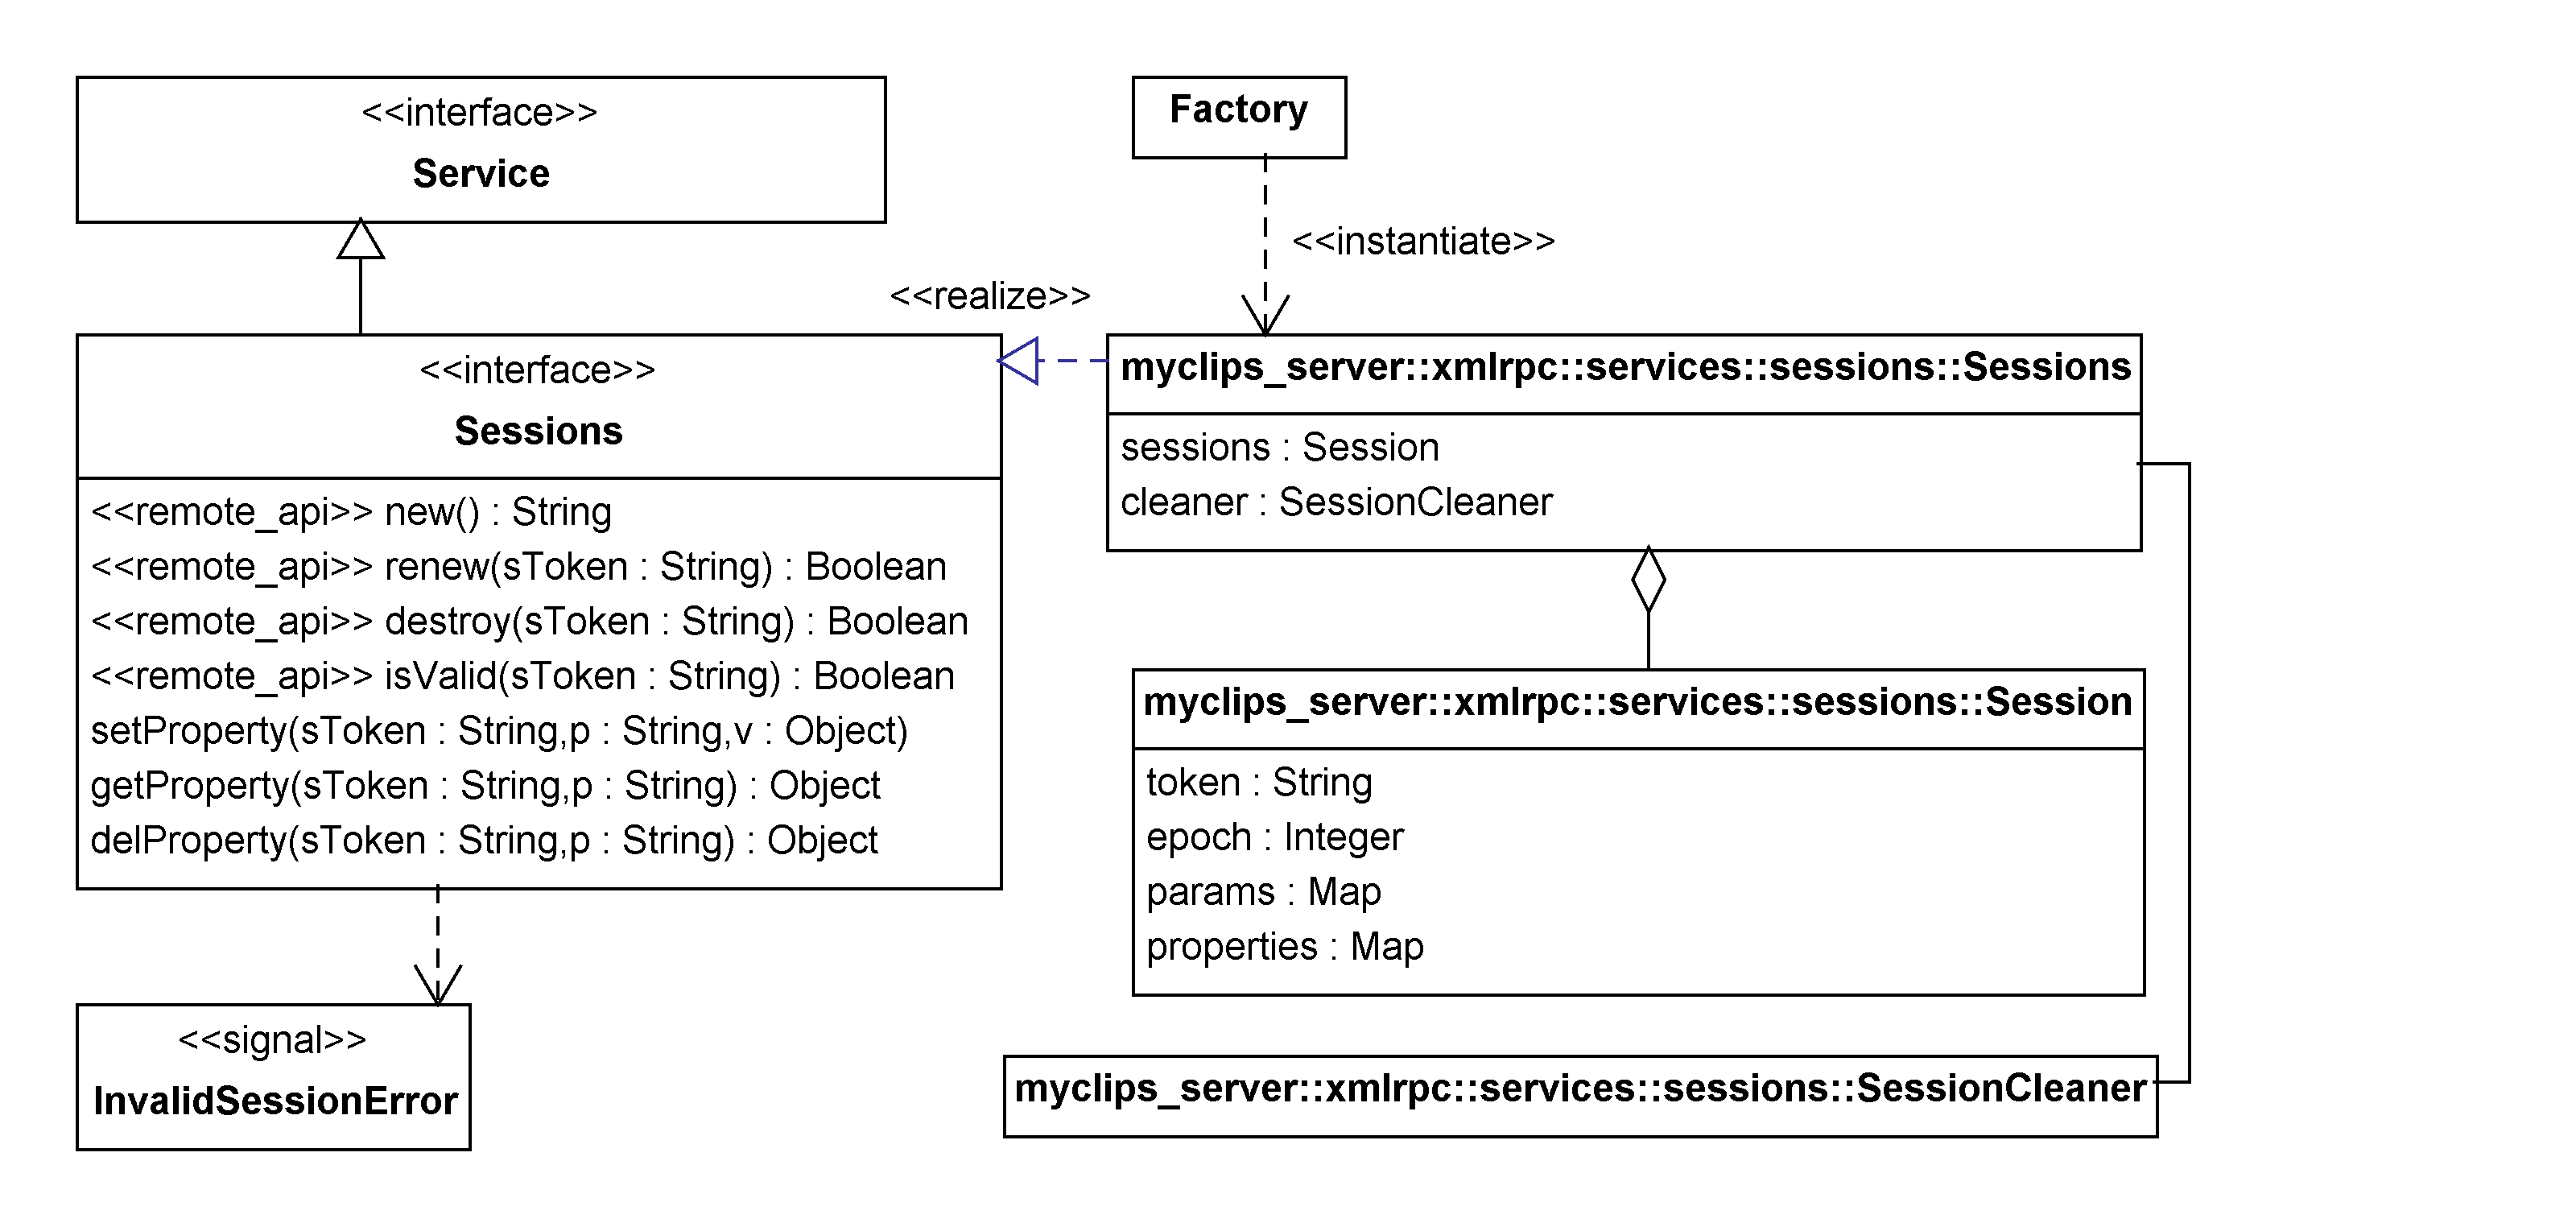
\includegraphics[width=1\textwidth]{Immagini/Capitolo3/Classi/myclips_server_services_Sessions.png}
\caption{Package \emph{myclips\_server.xmlrpc.services}: vista delle classi e interfacce relative al servizio \emph{Sessions}}\label{fig:class-myclips-server-services-sessions}
\end{figure}

Il servizio \emph{Sessions}~(\figurename~\ref{fig:class-myclips-server-services-sessions}) consente ai \emph{client} di creare sessioni persistenti fra più richieste successive. Ogni sessione viene inizializzata e gestita dalla classe concreta, che provvederà a memorizzarla fino a quando non verranno riscontrate condizioni favorevoli all'eliminazione.
Il servizio fornisce sia un'interfaccia rivolta ai client (per la creazione, rimozione e rinnovo delle sessioni), sia ad altri servizi del sistema (per realizzare un meccanismo di stoccaggio persistente delle informazioni).


\subsubsection{Servizio Registro di tipi}

\begin{figure}[h]
\centering
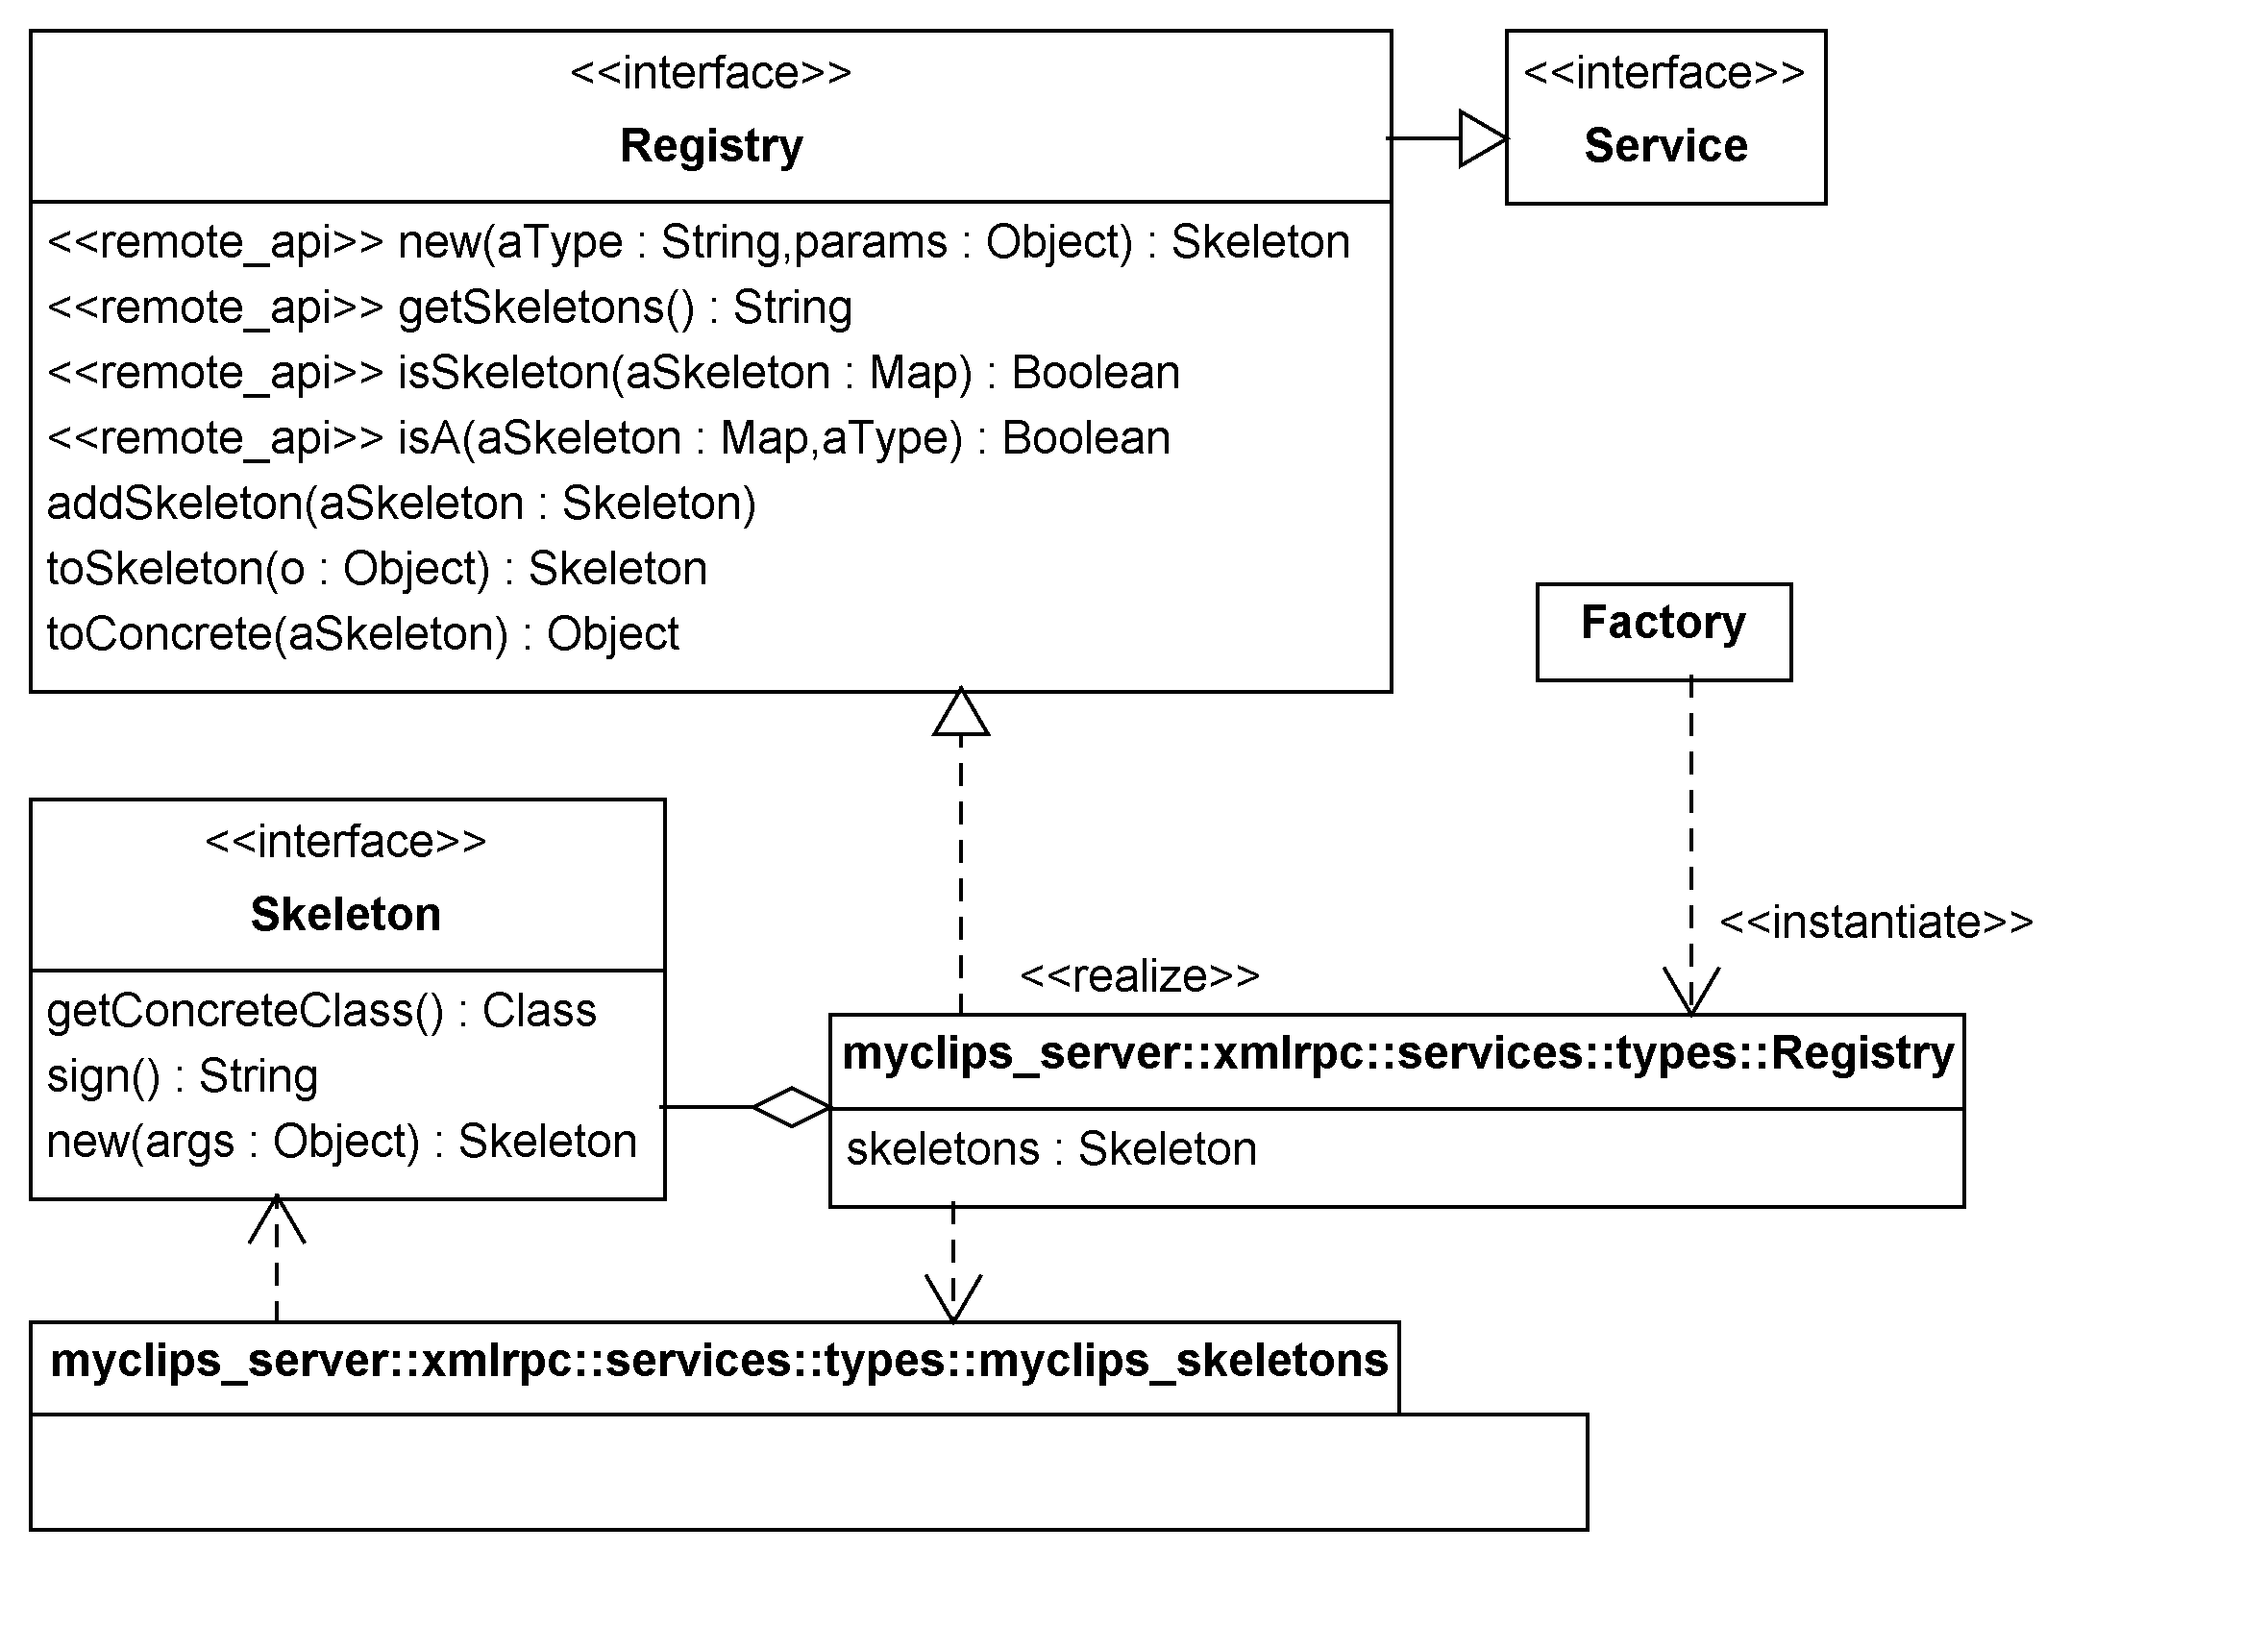
\includegraphics[width=1\textwidth]{Immagini/Capitolo3/Classi/myclips_server_services_Registry.png}
\caption{Package \emph{myclips\_server.xmlrpc.services}: vista delle classi e interfacce relative al servizio \emph{Registry}}\label{fig:class-myclips-server-services-registry}
\end{figure}

Il servizio \emph{Registry}~(\figurename~\ref{fig:class-myclips-server-services-registry}) consente, a client e altri servizi, di manipolare tipi complessi non previsti da specifiche implementazioni del protocollo di trasmissione dei messaggi fra \emph{client} e \emph{server}. Le attività svolte dal servizio sono quelle di organizzare una collezione di classi \emph{Skeleton} che forniscano i metodi di conversione da classi specifiche a forme di più facile trasmissione e viceversa.
Il servizio offre anche la possibilità ad altre parti del sistema di registrare tipi di \emph{Skeleton} personalizzati.

L'implementazione concreta dell'interfaccia del servizio, realizzata dalla classe \emph{Registry}, utilizza una collezione di \emph{Skeleton} riuniti nel \emph{sub-package} \emph{myclips\_server.xmlrpc.services.types.myclips\_skeletons} per rappresentare costrutti e tipi utilizzati dal motore inferenziale.

\subsubsection{Servizio Client IO}

\begin{figure}[h]
\centering
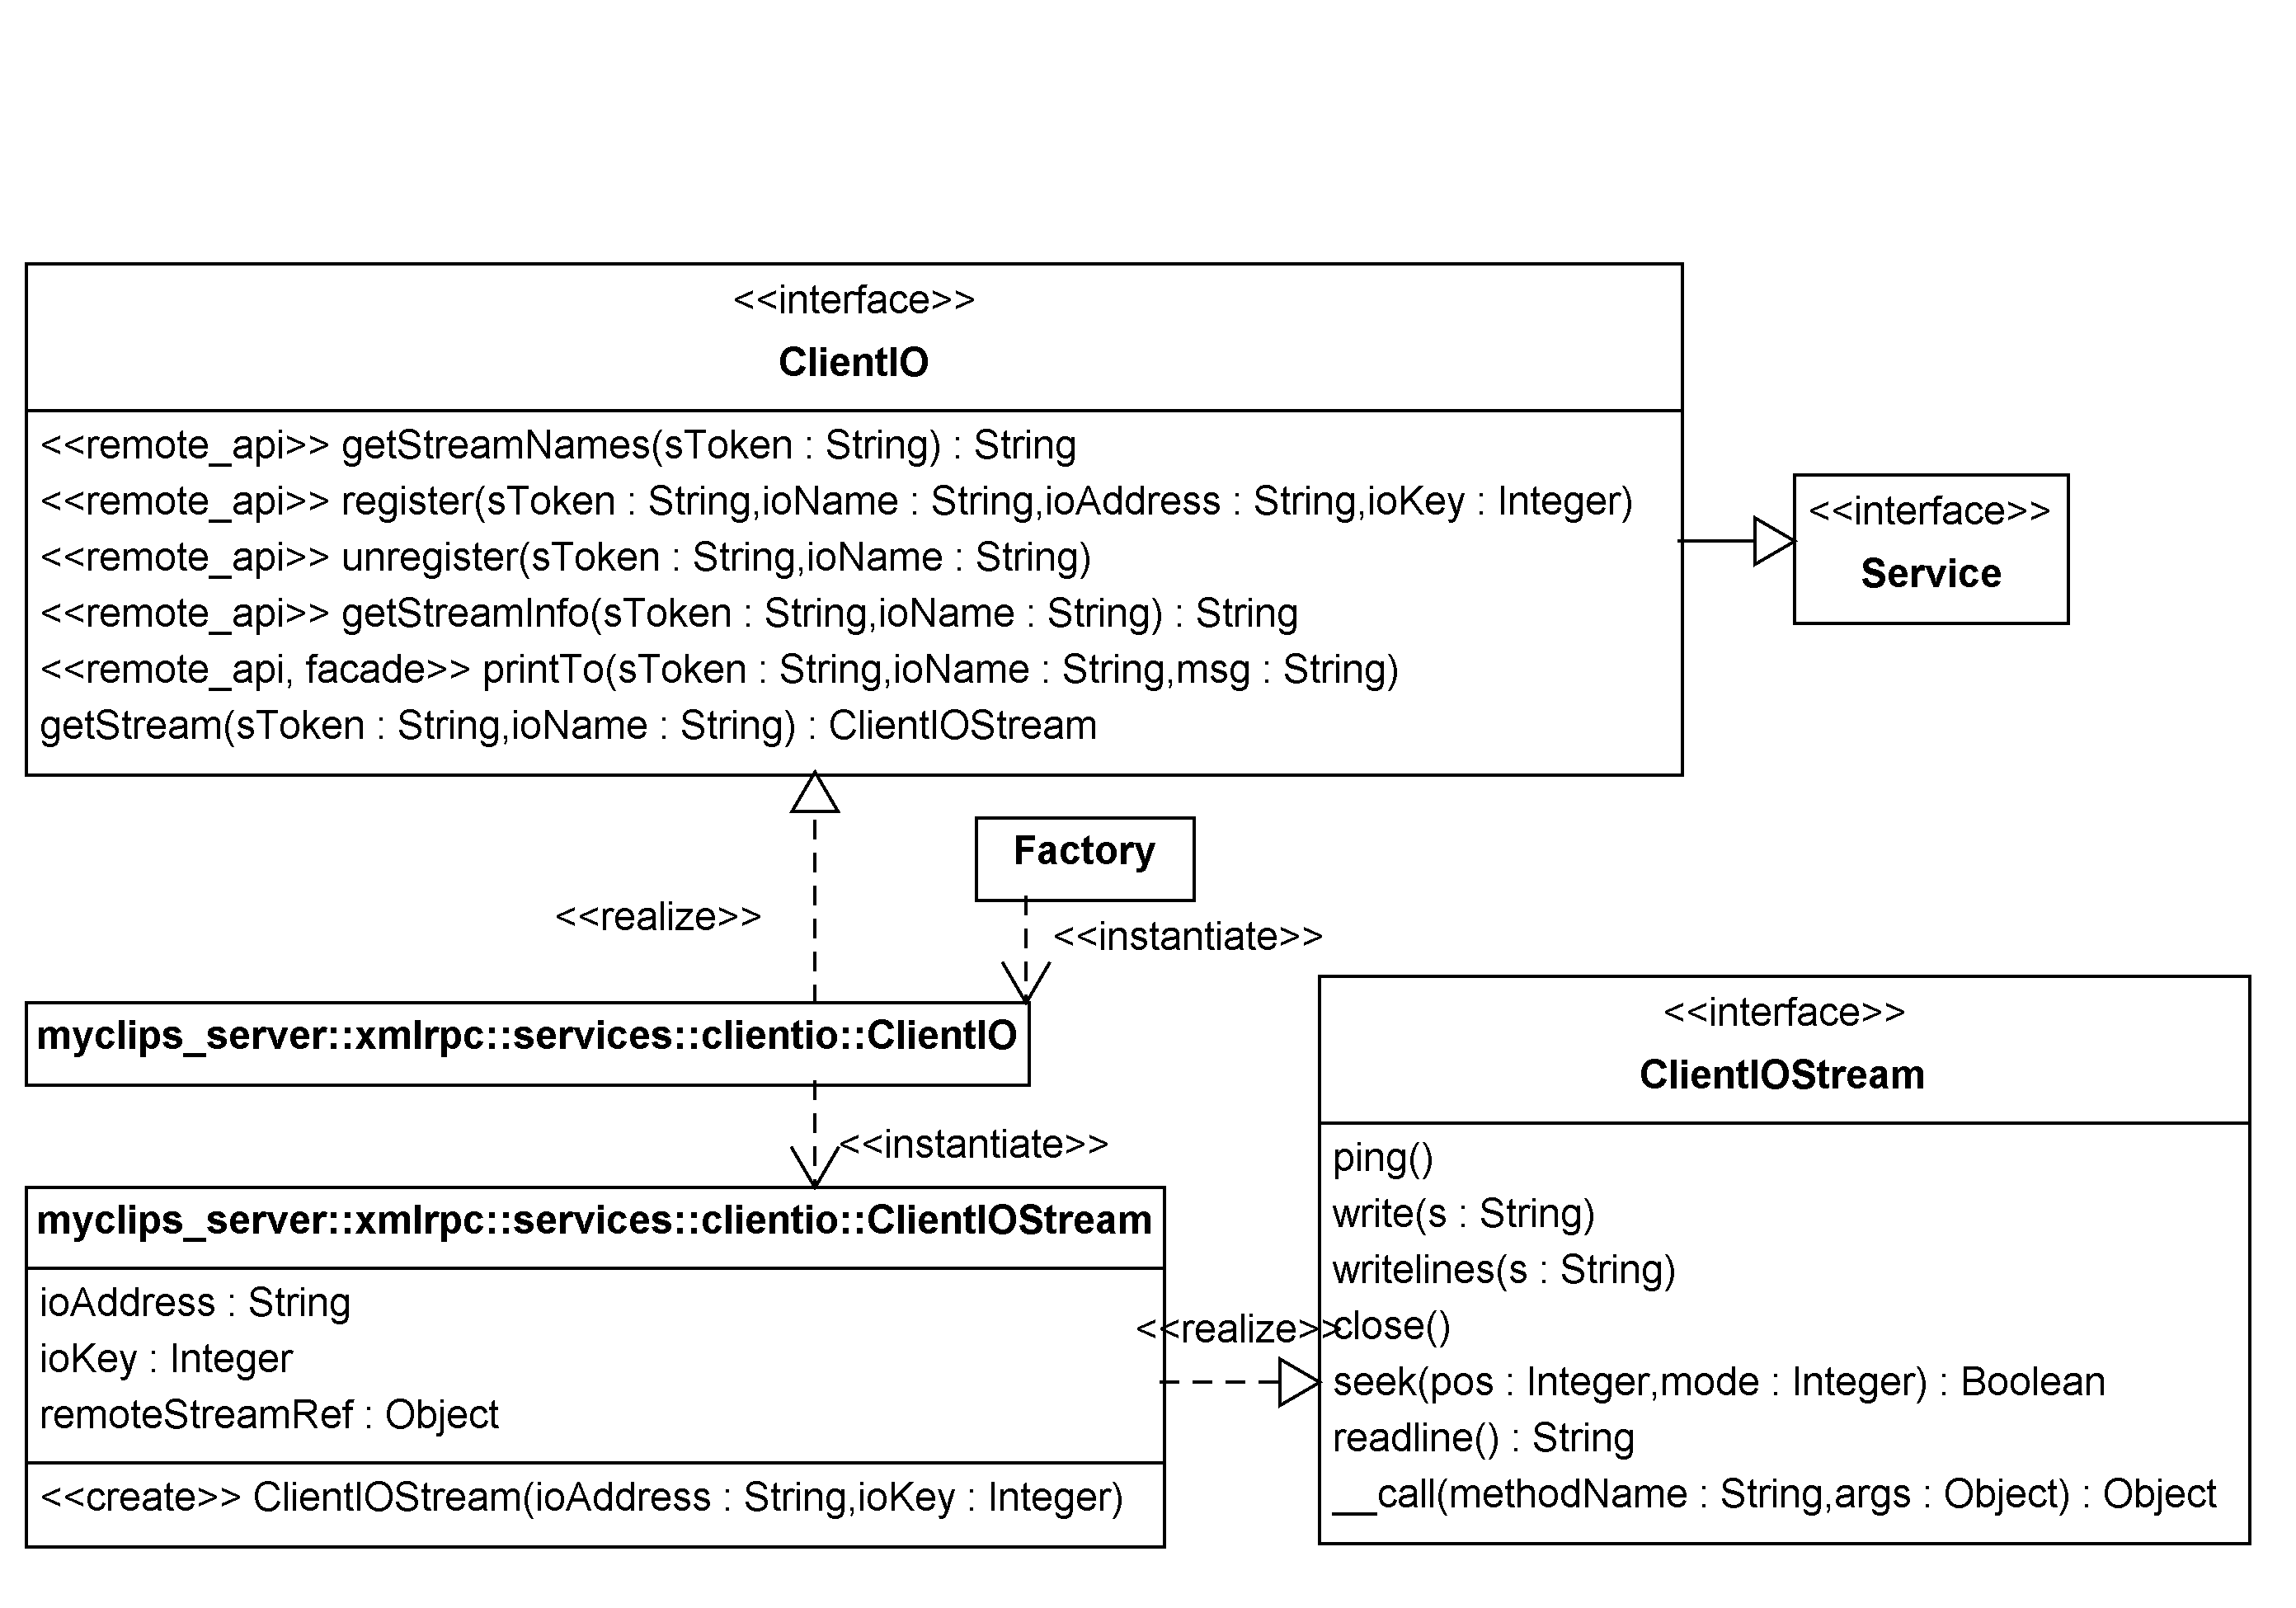
\includegraphics[width=1\textwidth]{Immagini/Capitolo3/Classi/myclips_server_services_ClientIO.png}
\caption{Package \emph{myclips\_server.xmlrpc.services}: vista delle classi e interfacce relative al servizio \emph{ClientIO}}\label{fig:class-myclips-server-services-clientio}
\end{figure}

Il servizio \emph{ClientIO}~(\figurename~\ref{fig:class-myclips-server-services-clientio}) permette ai client di fornire i parametri di utilizzo relativi a stream remoti che il server  (e i relativi servizi) può utilizzare in sostituzione degli stream locali. L'utilizzo degli stream remoti consente di dirottare tutte le normali operazioni di scrittura e lettura, eseguite all'interno del motore inferenziale, verso le risorse messe a disposizione dal client in maniera trasparente.
Al client viene richiesta l'implementazione di un'interfaccia analoga a \emph{ClientIOStream}.

\subsubsection{Servizio Remote Shell}

\begin{figure}[h]
\centering
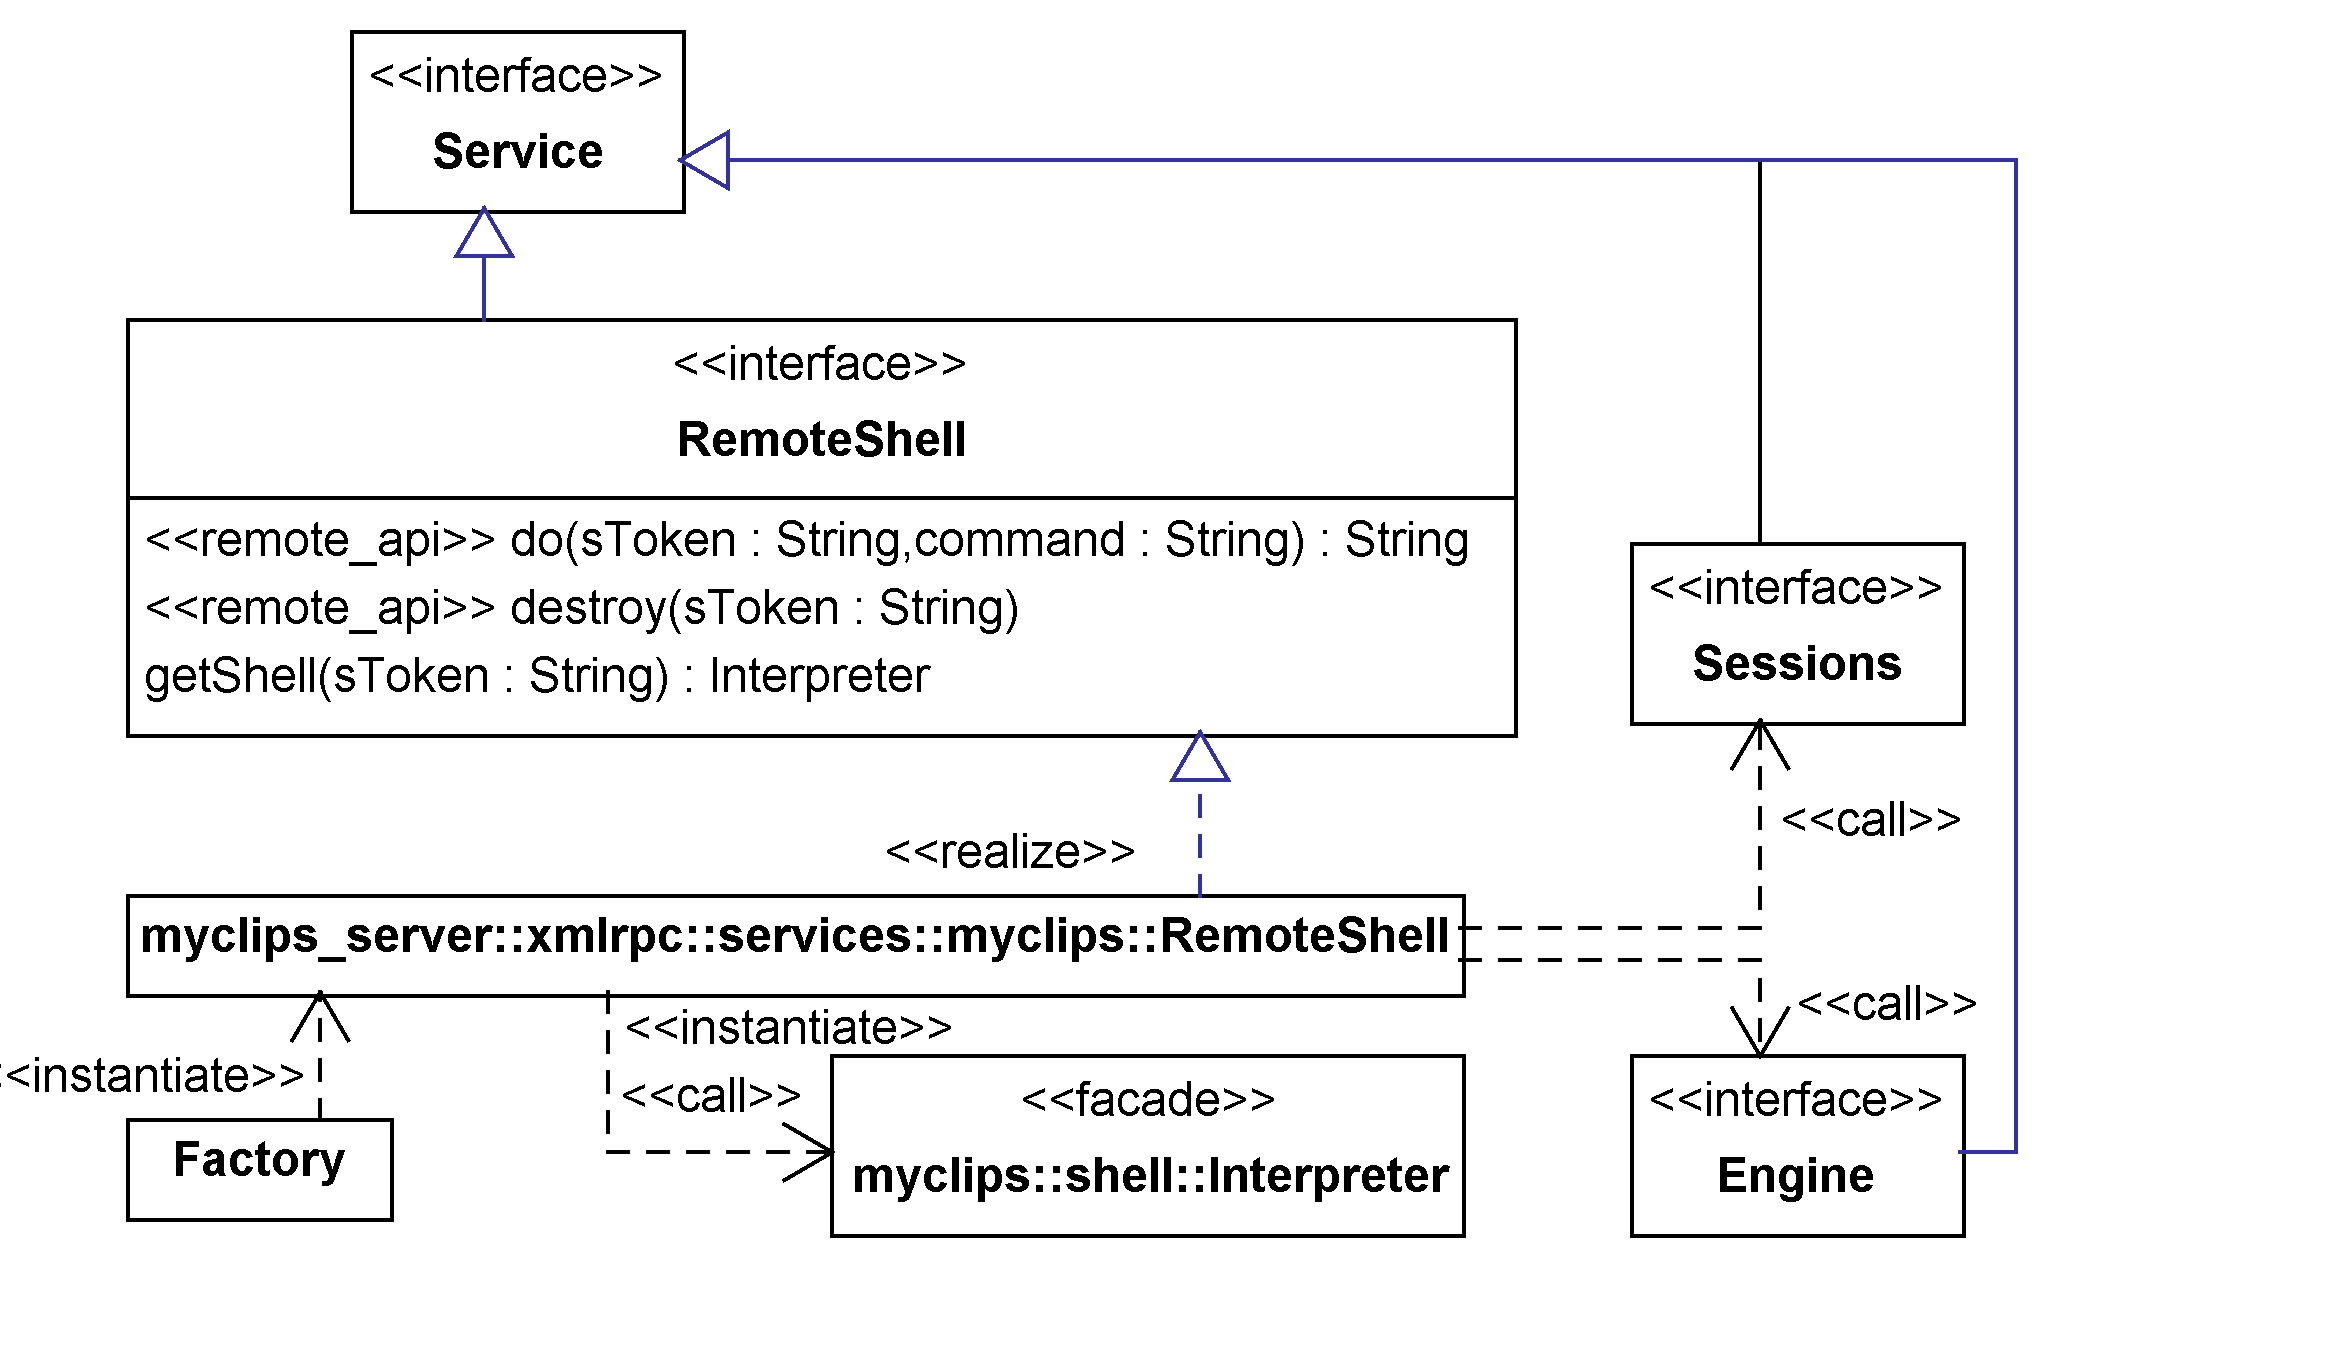
\includegraphics[width=1\textwidth]{Immagini/Capitolo3/Classi/myclips_server_services_RemoteShell.png}
\caption{Package \emph{myclips\_server.xmlrpc.services}: vista delle classi e interfacce relative al servizio \emph{RemoteShell}}\label{fig:class-myclips-server-services-remoteshell}
\end{figure}

Il servizio \emph{RemoteShell}~(\figurename~\ref{fig:class-myclips-server-services-remoteshell}) viene utilizzato per distribuire i servizi del modulo Interprete del sistema principale: attraverso lo scambio di comandi, trasferiti come stringhe di testo, è possibile manipolare istanze remote del motore inferenziale in maniera esattamente analoga a quanto avviene tramite l'utilizzo di un \emph{Terminale} locale.

Il servizio fa uso delle interfacce \emph{Sessions} (per memorizzare l'istanza \emph{Interpreter}), \emph{Engine} (per l'infrastruttura necessaria all'\emph{Interpreter}) e di \emph{ClientIO} (per l'inoltro dei flussi \emph{input/output}).

\subsubsection{Servizio Engine}

\begin{figure}[h]
\centering
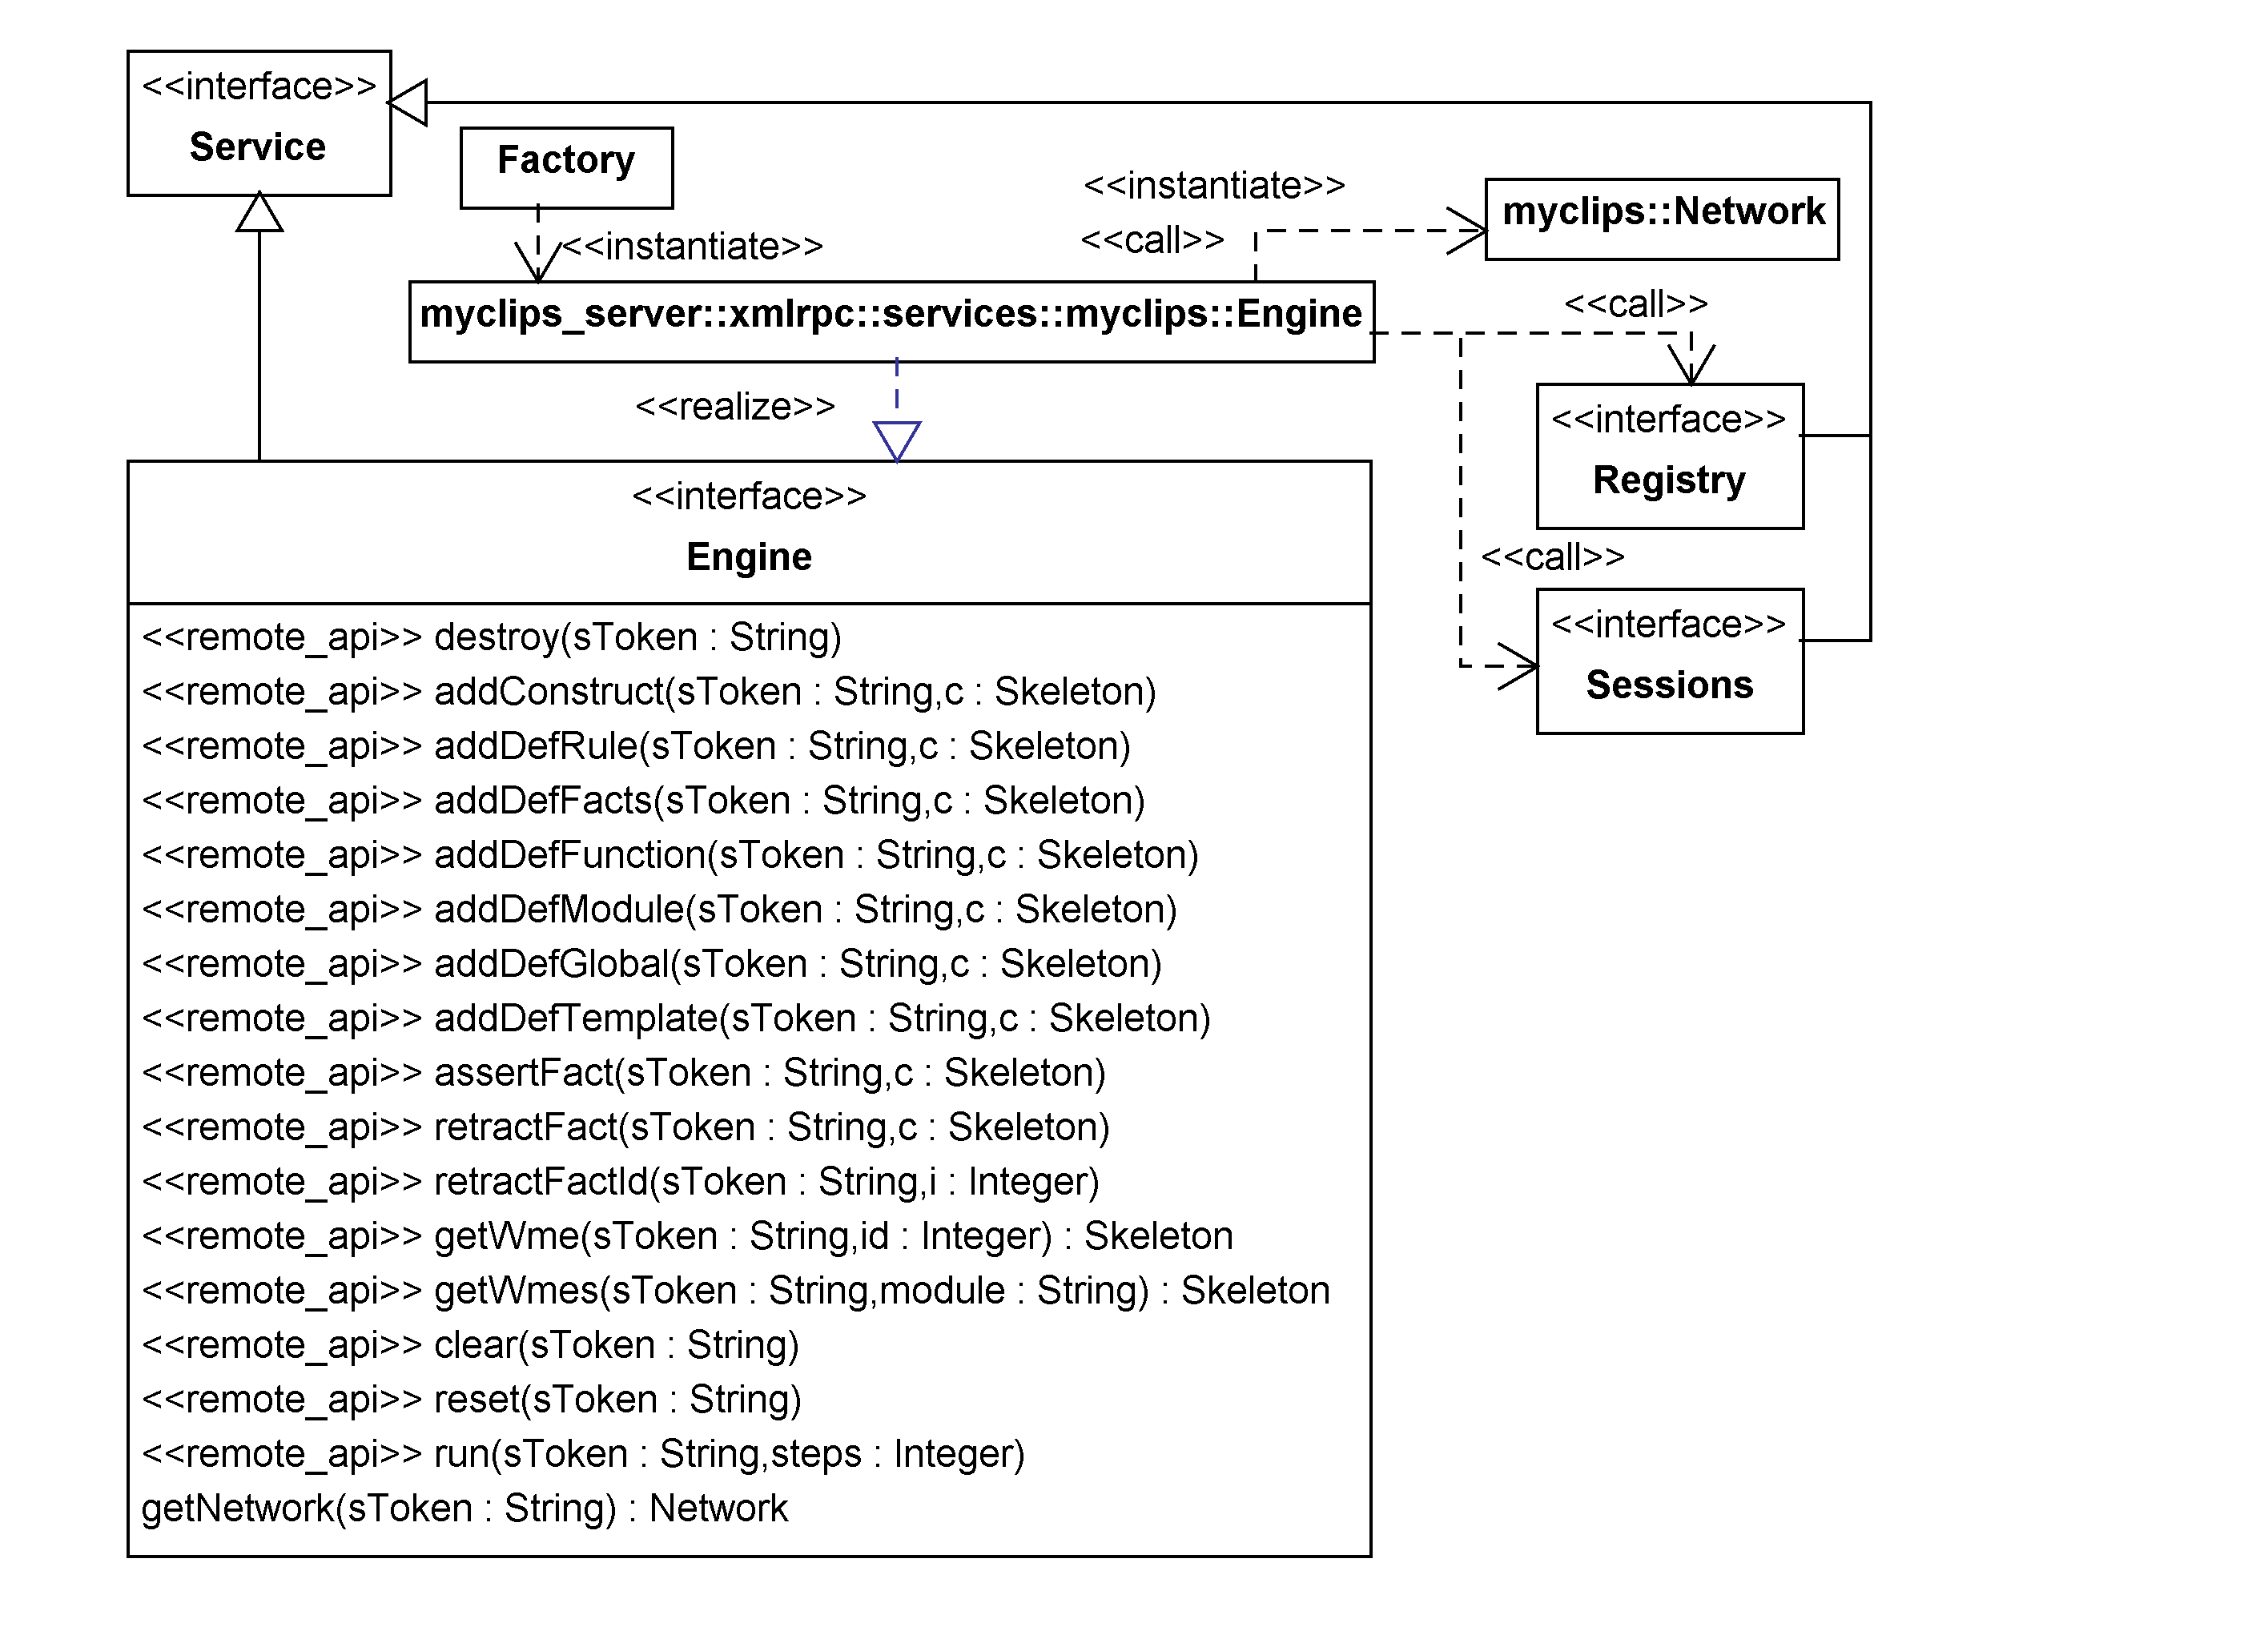
\includegraphics[width=1\textwidth]{Immagini/Capitolo3/Classi/myclips_server_services_Engine.png}
\caption{Package \emph{myclips\_server.xmlrpc.services}: vista delle classi e interfacce relative al servizio \emph{Engine}}\label{fig:class-myclips-server-services-engine}
\end{figure}

Il servizio che realizza il collegamento fra \emph{client} e il motore inferenziale prende il nome di \emph{Engine}~(\figurename~\ref{fig:class-myclips-server-services-engine}). Utilizzando i metodi pubblicizzati tramite l'interfaccia di servizio \emph{Engine}, al client viene data la possibilità di inizializzare il motore inferenziale aggiungendo costrutti (opportunamente creati tramite l'utilizzo del servizio \emph{Registry}), eseguire il ciclo \emph{recognize-act} e, utilizzando i metodi di ispezione forniti, analizzare lo stato finale del sistema. Tramite l'utilizzo dei servizi \emph{ClientIO} e \emph{ClientEvents}, il motore offre la stessa gamma di funzionalità utilizzabili attraverso un'istanza locale del sistema. La classe concreta che realizza il servizio si affida all'utilizzo dei metodi offerti dalla classe del core \emph{Network}.

\subsection{Terminale}

\begin{figure}[h]
\centering
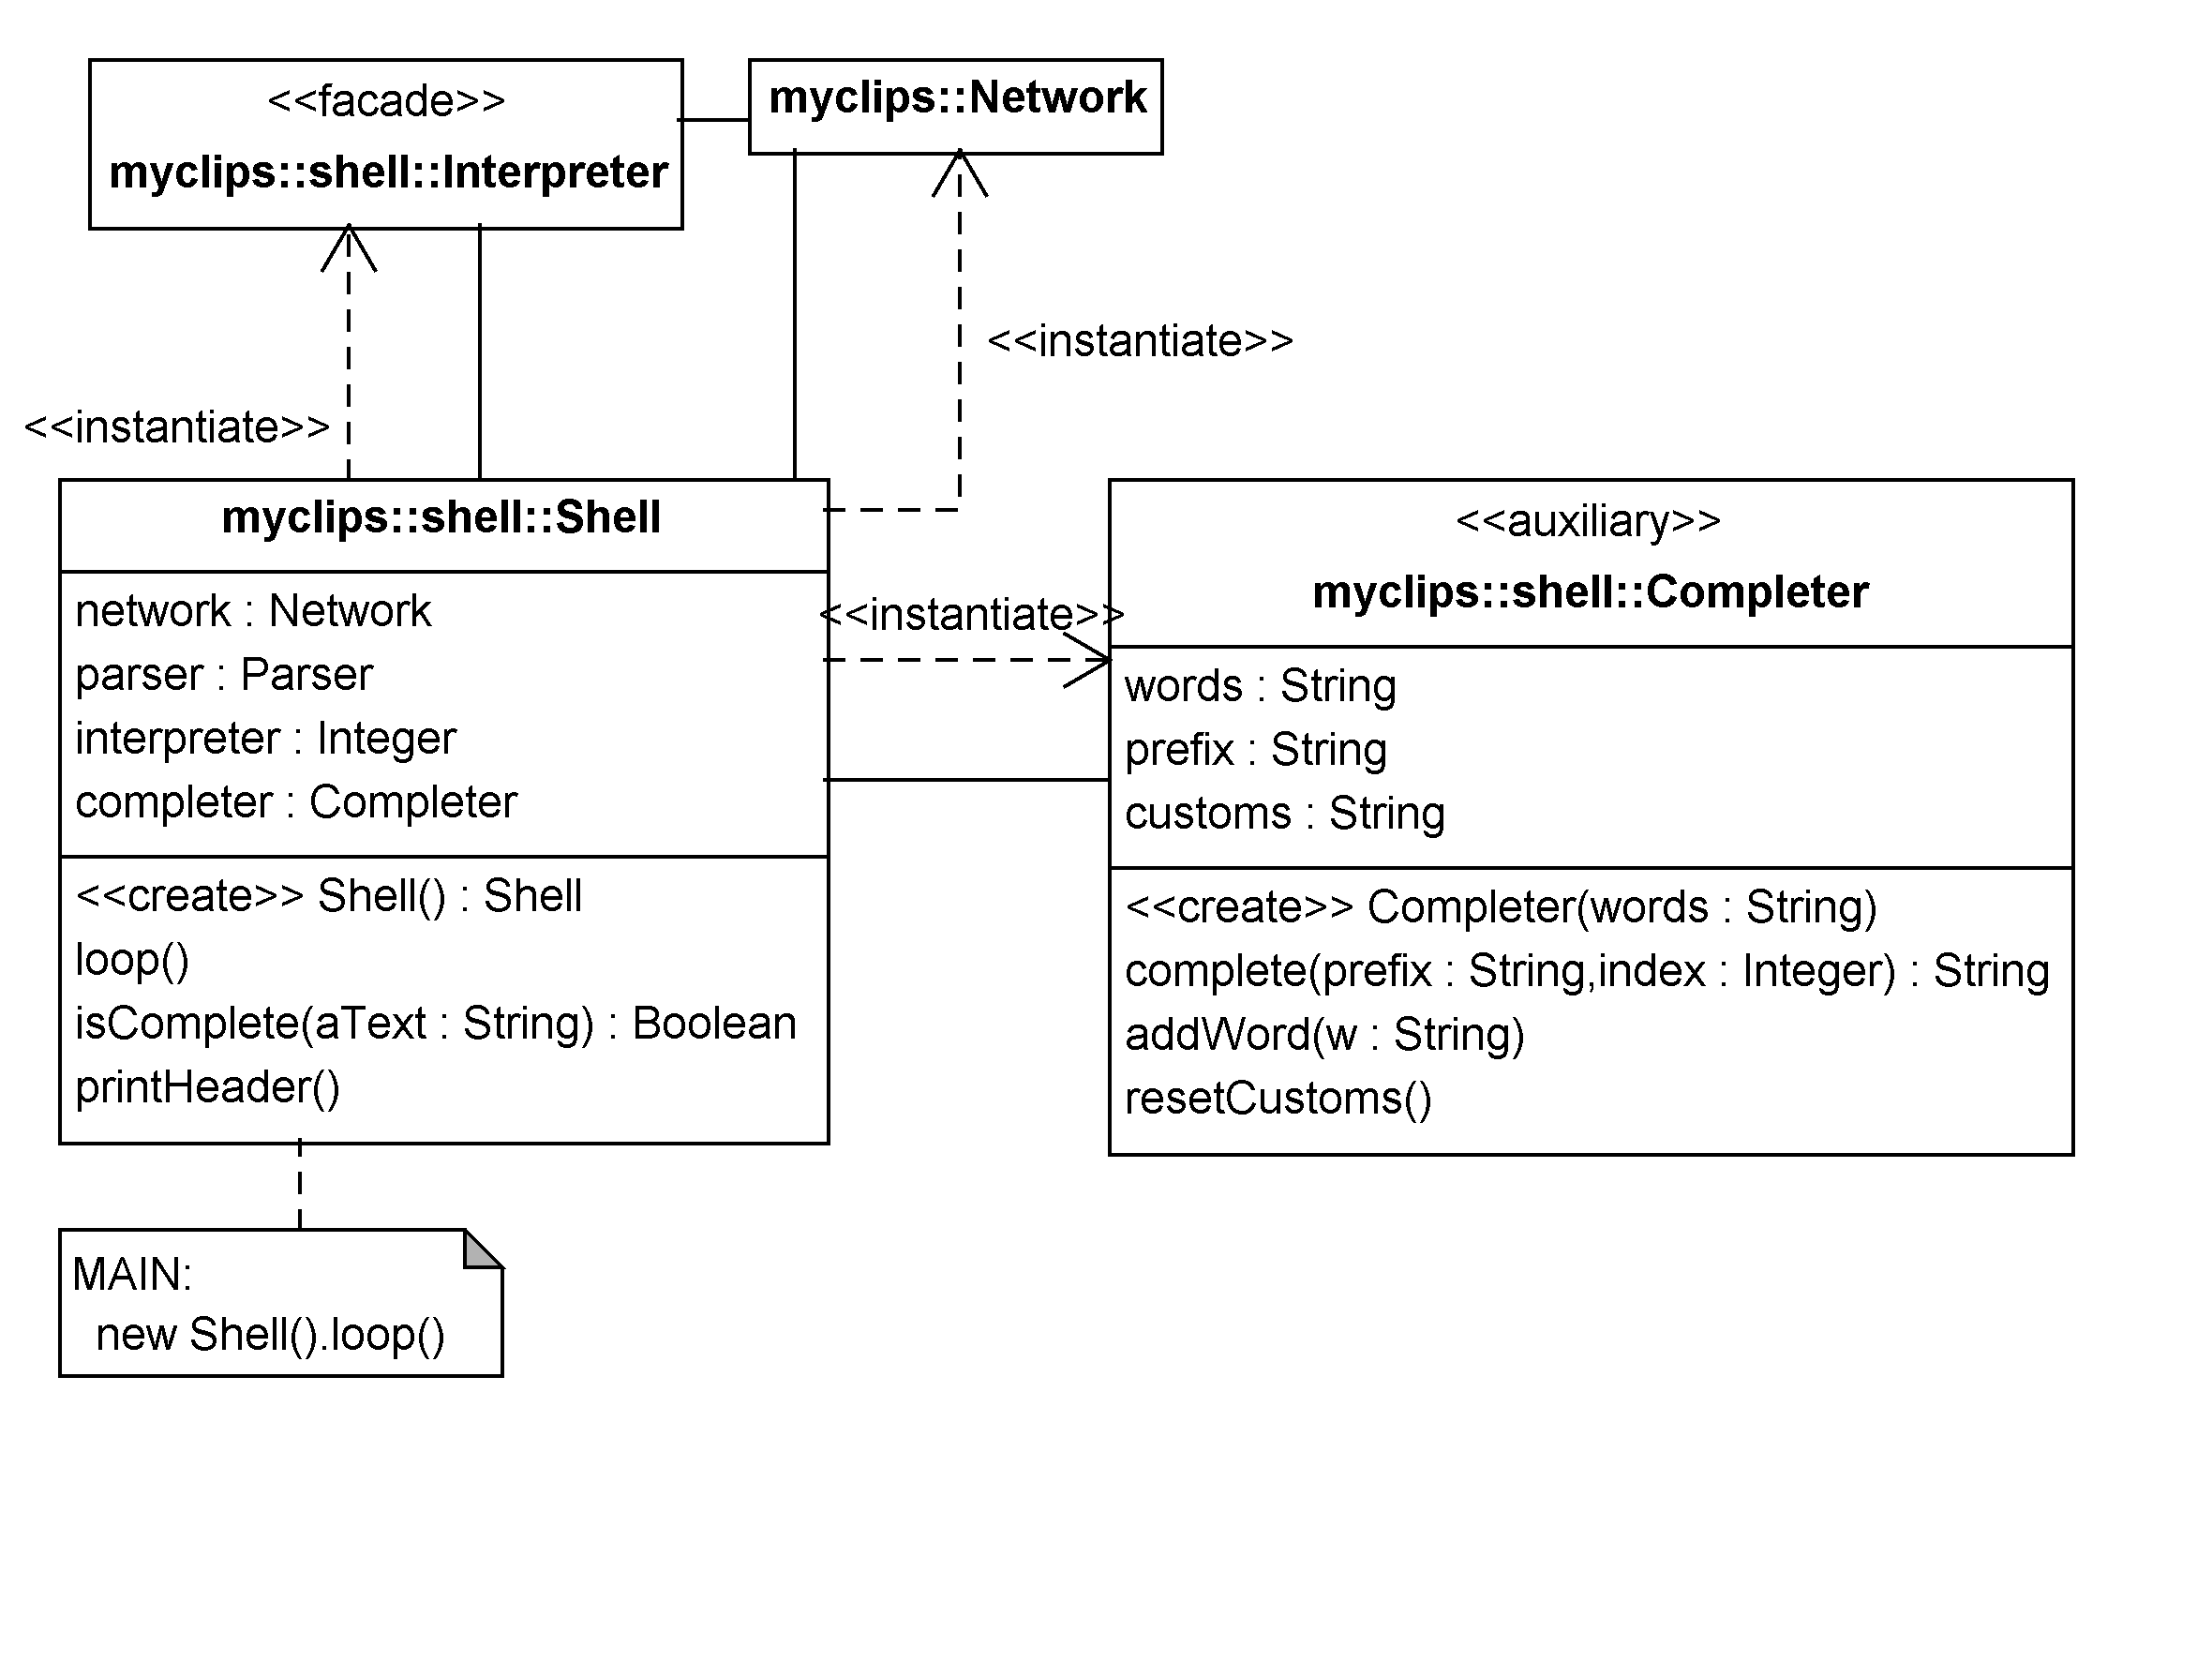
\includegraphics[width=1\textwidth]{Immagini/Capitolo3/Classi/myclips_shell_Shell.png}
\caption{Package \emph{myclips.shell}: vista delle classi relative al \emph{Terminale}}\label{fig:class-myclips-shell-Shell}
\end{figure}

L'interfaccia Terminale offerta dal sistema viene implementata tramite la collaborazione di due classi presenti nel \emph{package} \emph{myclips.shell}: \emph{Shell} e \emph{Completer}.~(\figurename~\ref{fig:class-myclips-shell-Shell})
La prima realizza il ciclo principale di immissione e valutazione dei comandi testuali forniti dall'utente, utilizzando le funzionalità di \emph{Interpreter}, la seconda valuta il completamento automatico delle immissioni dell'utente, quando richiesto dalla pressione di un tasto speciale.


\section{Implementazione}

La fase di implementazione ha richiesto la conversione delle strutture progettate e mostrate nei paragrafi precedenti tramite l'utilizzo di un linguaggio di programmazione. Inoltre è stata necessaria la selezione del protocollo da utilizzare per le comunicazioni \emph{client-server}.

\subsection{Scelta del linguaggio: Python}

\begin{figure}[h]
\centering
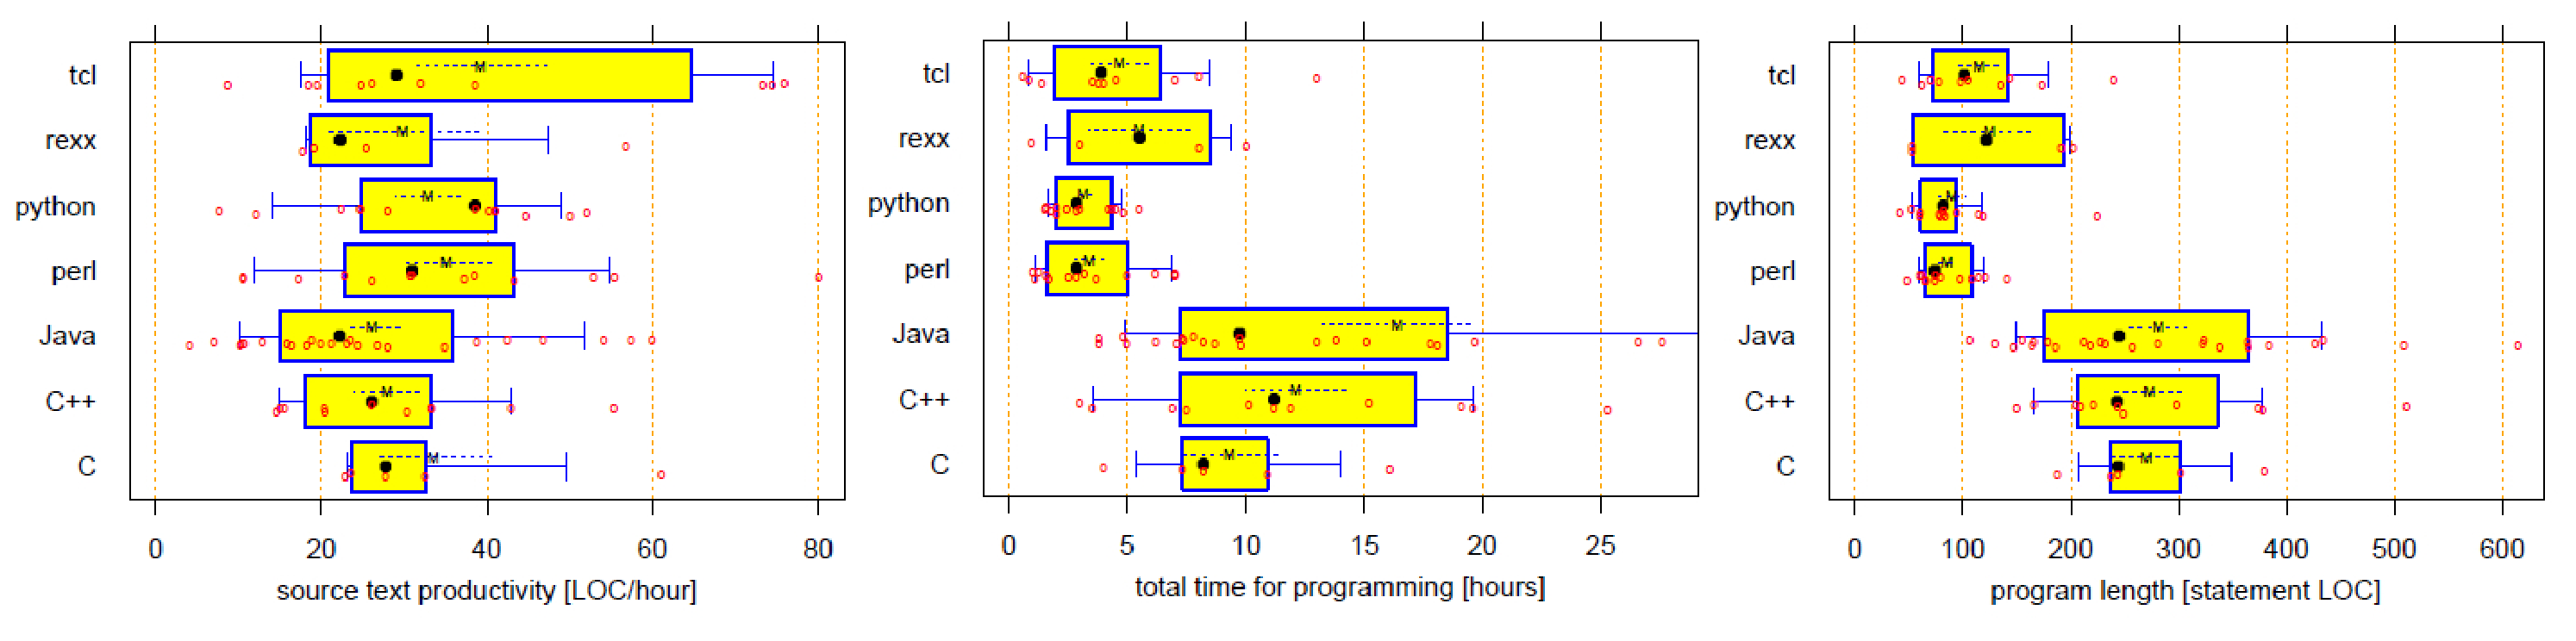
\includegraphics[viewport=0 0 1434 347, width=1\textwidth]{Immagini/Capitolo3/Python-comparison.pdf}
\caption[Comparazione fra Python e altri linguaggi di programmazione]{Comparazione fra Python e altri linguaggi di programmazione mostrando, da sinistra a destra, velocità di produzione del codice, tempo totale di produzione e lunghezza degli artefatti~\cite{prechelt2000}.}\label{fig:python-comparison}
\end{figure}

La scelta del linguaggio di programmazione da utilizzare per l'implementazione del sistema è ricaduta su linguaggio intepretato \emph{Python}\footnote{http://www.python.org/}. A supporto della scelta si propongono le seguenti argomentazioni:
\begin{description}
	\item[Gratuità:] Python è un linguaggio open-source utilizzabile, modificabile e distribuibile gratuitamente. Lo sviluppo del linguaggio è affidato ad una organizzazione \emph{no-profit} (Python Software Foundation)~\cite{pythonfaq}.
	
	\item[Facilità di sviluppo:] Python è un linguaggio di programmazione \emph{general-purpose} di alto livello. La grande varietà di librerie distribuite insieme alle implementazioni del linguaggio (con ambiti che variano dalla programmazione asincrona alla gestione degli archivi zip~\cite{pythonfaq}~\cite{pythonstdlib}) o prodotte dalla comunità\footnote{http://pypi.python.org/pypi} consente di utilizzare le soluzioni offerte per velocizzare i processi di sviluppo degli artefatti~\cite{prechelt2000}~\cite{prashant2008}.
	
	\item[Sinteticità del linguaggio:] studi comparativi fra linguaggi di programmazione attualmente disponibili (\figurename~\ref{fig:python-comparison}) hanno evidenziato la proprietà del linguaggio di utilizzare una sintassi concisa senza ridurre le capacità espressive~\cite{prechelt2000}~\cite{prashant2008}.
	
	\item[Meccanismi di riflessione:] il linguaggio integra dei meccanismi di riflessione e caricamento a \emph{run-time} avanzati che rendono agevole la realizzazione dei meccanismi di estensione dell'environment progettato. Le attività di inclusione di nuove funzioni di sistema o strategie CRS si riducono alla semplice serializzazione degli algoritmi, senza la necessità di eseguire fasi di compilazione o integrazione complesse.
	
	\item[Multi-piattaforma:] il supporto al linguaggio è disponibile per numerose piattaforme e sistemi operativi~\cite{pythonfaq} (compresi quelli richiesti per il  soddisfacimento del \emph{Vincolo-6}).
	
	\item[Capacità di integrazione:] sono disponibili numerose implementazioni di Python (con diversi livelli di compatibilità), realizzate in linguaggi come  Java\footnote{http://www.jython.org/}, C\#\footnote{http://ironpython.net/}, C\footnote{Implementazione di riferimento: http://www.python.org/}. Ognuna consente un'integrazione diretta con meccanismi propri del linguaggio di implementazione. In aggiunta, le capacità offerte dalle librerie permettono di utilizzare meccanismi di integrazione agnostici tra linguaggi eterogenei.
\end{description}

%Come rovescio della medaglia, la scelta ha determinato alcuni effetti sulle prestazioni complessive del sistema: nonostante le prestazioni teoricamente migliori ottenibili con linguaggi alternativi, il \emph{Vincolo-7} risulta egualmente soddisfatto. Le ridotte prestazioni offerte da Python (se messo in relazione con altri linguaggi), non sono state ritenute una ragione sufficiente ad invalidare la preferenza espressa, soprattutto tenendo conto dei vantaggi alternativi che la soluzione offre.

\subsection{Protocollo: XML-RPC}

\emph{Remote Procedure Call}, o \emph{RPC}, è un meccanismo tramite il quale un'applicazione posizionata su una \emph{macchina} richiede l'utilizzo di servizi forniti da un'altra applicazione residente su una \emph{macchina} differente. Con il termine \emph{macchina} non viene unicamente inteso un \emph{host}, un'installazione fisicamente separata, ma anche un processo residente in una porzione di memoria indipendente e che rende l'accesso alle risorse del servizio impossibile se non tramite il meccanismo \emph{RPC}. 

Il meccanismo \emph{RPC} prevede che una prima applicazione possa inviare uno o più messaggi ad una applicazione differente per invocare delle procedure. L'applicazione ricevente ha la possibilità,  a sua volta, di inviare i risultati dell'elaborazione tramite un ulteriore messaggio verso applicazione richiedente~\cite{MERRICK:2006:misc}.

\emph{RPC} descrive un meccanismo generalizzato per l'invocazione di procedure remote, non una concreta implementazione di un protocollo o di tecnologie per lo scambio dei messaggi fra gli \emph{host}. Partendo dal concetto generale di \emph{RPC}, nel tempo sono state proposte differenti implementazioni basate su protocolli proprietari o codifiche dei messaggi differenti~\cite{JAIRATH:2004:misc}~\cite{dcerpc}.

\begin{figure}[h]
\centering
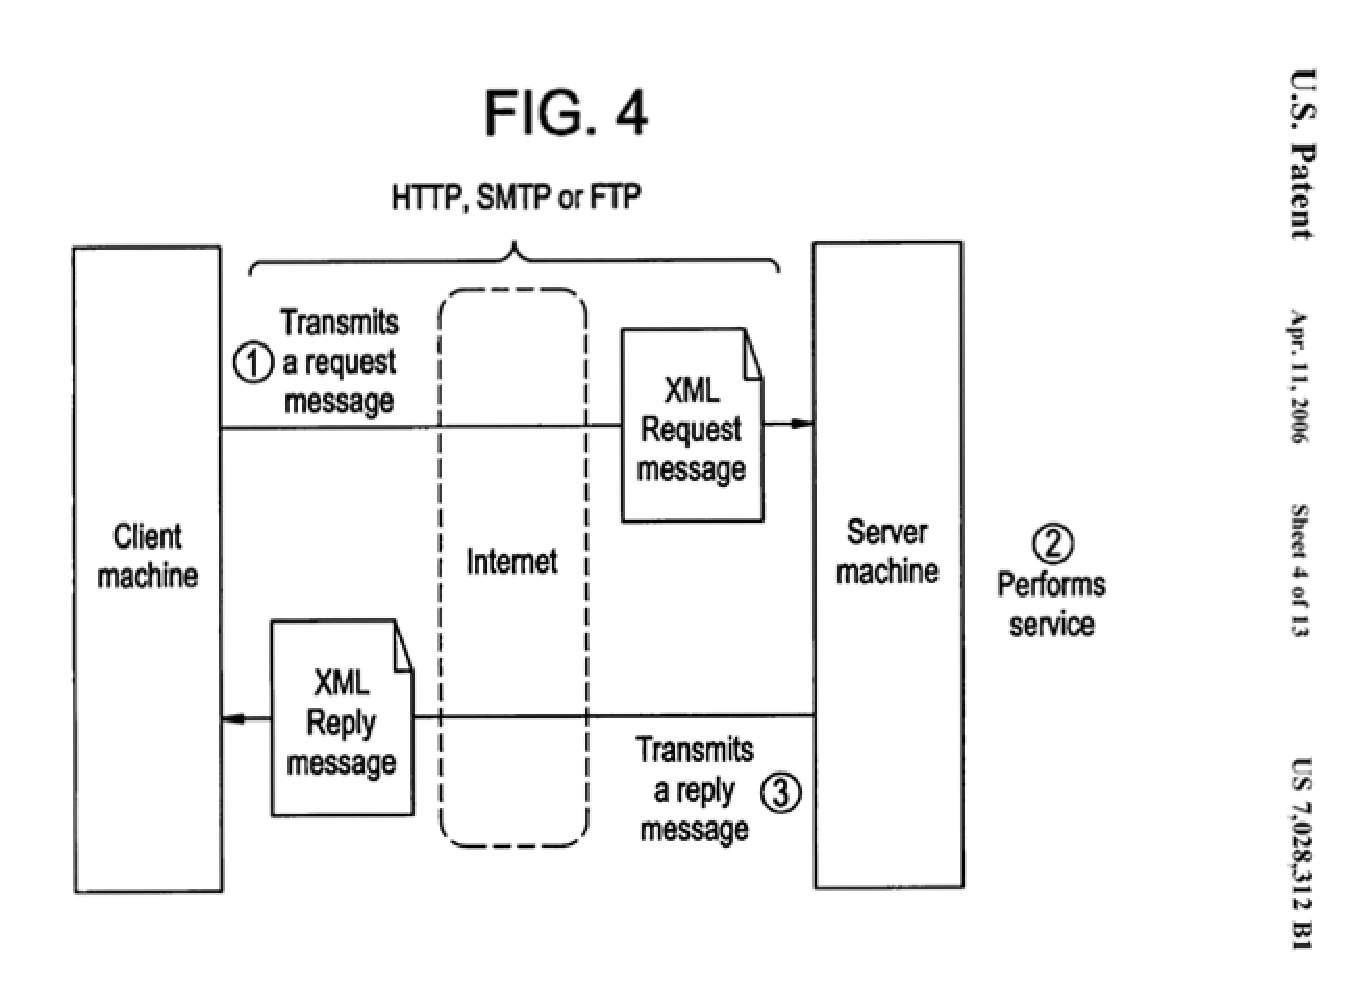
\includegraphics[scale=0.5, viewport=0 0 646 440]{Immagini/Capitolo3/XMLRPC-patent.pdf}
\caption[Comunicazione tramite \emph{XML-RPC}]{Comunicazione tramite \emph{XML-RPC}: immagine presente nella richiesta originale di brevetto~\cite{MERRICK:2006:misc}.}\label{fig:xmlrpc-patent}
\end{figure}

\emph{XML-RPC} è una fra le implementazioni proposte per \emph{RPC}: si propone come un meccanismo di chiamata a procedura remote semplice e versatile. Il brevetto originale con il quale è stato proposto descrive sia il meccanismo di chiamata, che un sistema per l'implementazione del metodo~\cite{MERRICK:2006:misc}.
\emph{XML-RPC} prevede lo scambio di richieste e risposte usando il formato \emph{XML}, attraverso meccanismi di trasporto multipli. Solitamente, con l'uso del termine \emph{XML-RPC} si è soliti però indicare il protocollo di scambio messaggi in \emph{XML} attraverso un meccanismo di trasporto basato sul protocollo \emph{HTTP}.

\begin{program}
\begin{verbatimtab}

POST /RPC2 HTTP/1.0
User-Agent: Frontier/5.1.2 (WinNT)
Host: betty.userland.com
Content-Type: text/xml
Content-length: 181


<?xml version="1.0"?>
<methodCall>
   <methodName>examples.getStateName</methodName>
   <params>
      <param>
         <value><i4>41</i4></value>
         </param>
      </params>
   </methodCall>
\end{verbatimtab}
\caption{Esempio di chiamata ad una procedura remota usando \emph{XML-RPC over HTTP}}\label{code:xmlrpc-request}
\end{program}

La codifica dei messaggi viene effettuata incapsulando i parametri di chiamata ed i valori di ritorno all'interno di appositi frammenti del documento \emph{XML}, i quali hanno il compito di attribuire una semantica alla stringa rappresentante il valore.

\begin{program}
\begin{verbatimtab}
HTTP/1.1 200 OK
Connection: close
Content-Length: 158
Content-Type: text/xml
Date: Fri, 17 Jul 1998 19:55:08 GMT
Server: UserLand Frontier/5.1.2-WinNT


<?xml version="1.0"?>
<methodResponse>
   <params>
      <param>
         <value><string>South Dakota</string></value>
         </param>
      </params>
   </methodResponse>
\end{verbatimtab}
\caption{Esempio di messaggi inviato a risposta di una chiamata a procedura remota usando \emph{XML-RPC over HTTP}}\label{code:xmlrpc-response}
\end{program}

I \emph{tag} che contengono il valore ne determinano il tipo. Nell'esempio fornito in Codice~\ref{code:xmlrpc-request}, il valore ''41'' (tipo \emph{integer}) viene incapsulato nel \emph{tag i4}. Il tag indica appunto che il tipo del valore, come da specifica, è un \emph{4 bytes signed integer}.

La specifica prevede la possibilità di utilizzare un set di tipi atomici con i quali rappresentare tutti i parametri di chiamata a procedura o i valori di ritorno (''integer'', ''string'', ''boolean'', ''double'', ''dateTime.iso8601'', ''base64'') e un gruppo di strutture composte (''struct'' per strutture analoghe a dizionari, ''array'' per vettori)~\cite{xmlrpcspec}.

A supporto della scelta di utilizzare \emph{XML-RPC} come protocollo RPC si propongono le seguenti argomentazioni:
\begin{description}
	\item[Semplicità:] il protocollo formalizza un metodo di interazione relativamente semplice se comparato con le alternative disponibili. Il trasferimento delle informazioni avviene nella forma di parametri di input o output di funzioni ed il modello di comunicazione non forza l'utilizzo di modelli di sicurezza complessi. La fornitura del servizio non richiede la necessità di creare descrizioni formali dello stesso, sebbene l'utilizzo di strumenti di supporto\footnote{XRDL: http://code.google.com/p/xrdl/} permettano la generazione automatica di client per i servizi.
	\item[Disponibilità:] l'utilizzo del protocollo è possibile in molti linguaggi di programmazione e piattaforme attraverso le implementazioni fornite da librerie apposite. Una stima approssimativa suggerisce la disponibilità di oltre 40 implementazioni differenti per un totale di oltre 25 piattaforme e linguaggi di programmazione~\cite{wikipedia-xmlrpc}.
\end{description}


\subsection{Tecnologie utilizzate}

\subsubsection{Pyparsing}
Pyparsing\footnote{http://pyparsing.wikispaces.com/home}$^,$\footnote{http://sourceforge.net/projects/pyparsing} è un modulo completamente scritto in linguaggio Python che fornisce un insieme di classi per la creazione di parser di espressioni, sia elementari che complesse e che prevedono l'uso di componenti variabili. Le espressioni sono combinate usando gruppi di operatori (come ad esempio ''+'' per definire la sequenzialità o ''$\mid$'' per le alternative), prevedendo l'utilizzo di espressioni replicate o ricorsive~\cite{pyparsing-gs}.

\begin{figure}[h]
\centering

\includegraphics[width=1\textwidth]{Immagini/Capitolo3/Classi/myclips_parser_PyParsing.png}
\caption[Integrazione di PyParsing nel modulo Parser]{Integrazione di PyParsing nel modulo Parser}\label{fig:class-myclips-parser-pyparsing}
\end{figure}

Il modulo Parser è stato implementato facendo uso delle classi fornite da Pyparsing per la definizione delle regole di valutazione. L'interfaccia \emph{ParserRule} mostrata nella descrizione del modulo Parser è stata sostituita dall'uso delle classi fornite da PyParsing. La classe principale \emph{Parser} è stata conseguentemente adattata per l'uso delle nuove istanze (\figurename~\ref{fig:class-myclips-parser-pyparsing})~\cite{pyparsing-apidoc}.

\subsubsection{BList}

\begin{figure}[h]
\centering
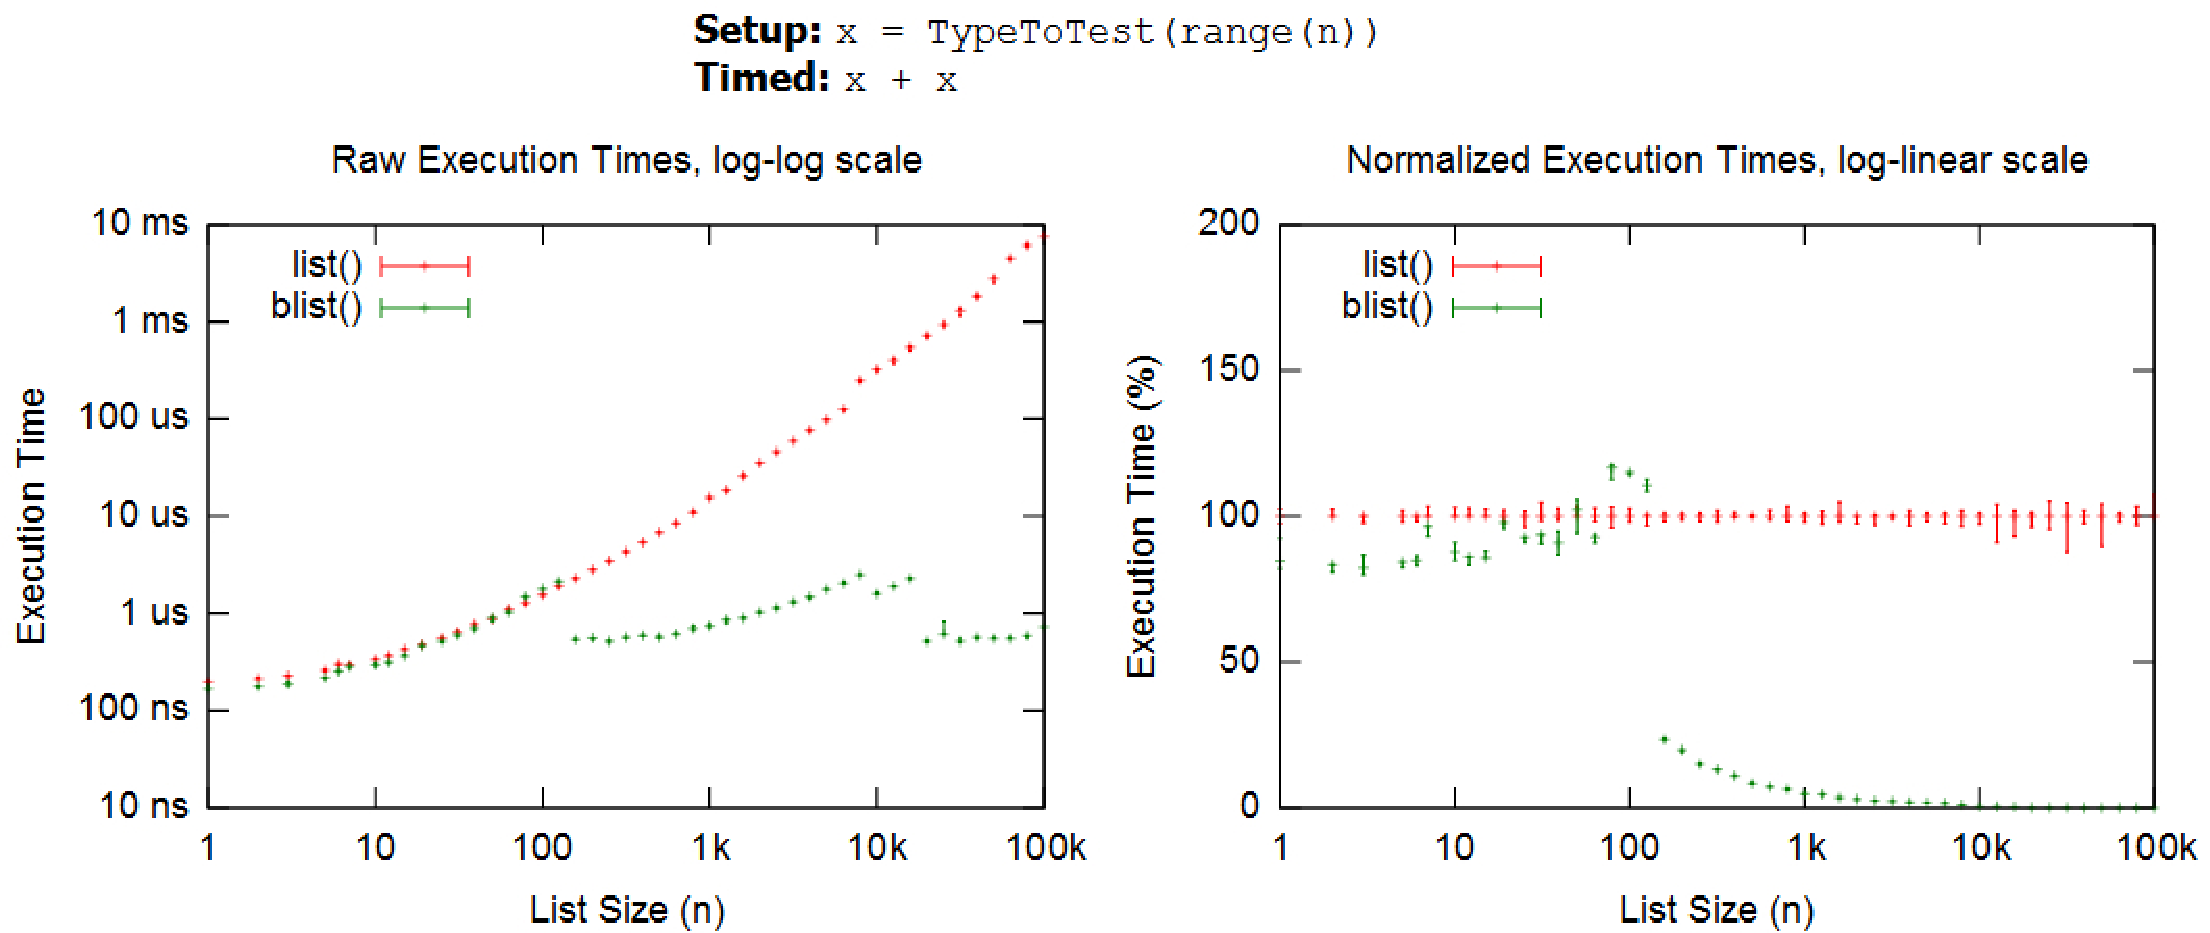
\includegraphics[width=1\textwidth]{Immagini/Capitolo3/BList-comparison.pdf}
\caption[Confronto fra l'implementazione di vettori fornita da BList e di \emph{default}]{Confronto fra l'implementazione di vettori fornita da BList e quella di \emph{default} fornita da CPython: prestazioni dell'operazione di inserimento~\cite{blist-prest}.}\label{fig:blist-comparison}
\end{figure}

La libreria BList\footnote{http://stutzbachenterprises.com/blist/} è un modulo Python per la sostituzione trasparente dell'implementazione delle collezioni fornite dal linguaggio~\cite{blist-manual}. Fornisce prestazioni superiori rispetto all'implementazione \emph{standard} dei vettori durante la manipolazione di collezioni di grandi dimensioni e fornisce realizzazioni di liste ordinate (\figurename~\ref{fig:blist-comparison})~\cite{blist-prest}.

Le liste ordinate fornite da Blist sono state utilizzate nell'implementazione delle strategie CRS \emph{Mea} e \emph{Lex} per l'inserimento ordinato delle attivazioni nell'agenda.


\subsubsection{NetworkX}

\begin{figure}
\centering
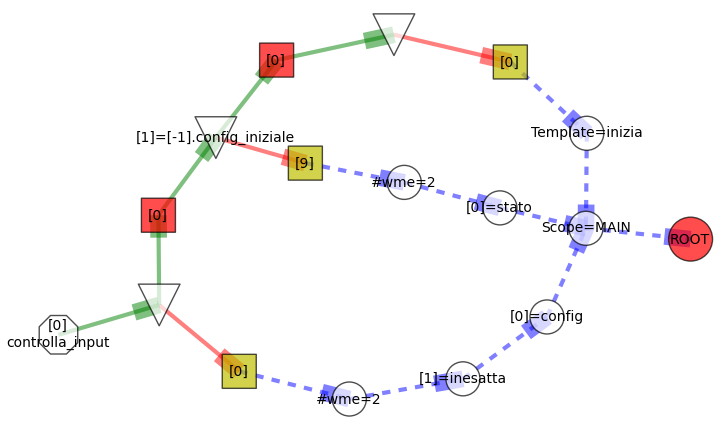
\includegraphics[width=1\textwidth]{Immagini/Capitolo3/draw-circuit.png}
\caption[Esempio d'uso della libreria NetworkX]{Esempio d'uso della libreria NetworkX per la rappresentazione del circuito compilato ottenuto dalla regola \emph{controlla\_input} in Codice~\ref{code:agricoltore-1}}\label{fig:networkx-example}
\end{figure}

NetworkX\footnote{http://networkx.lanl.gov/} è un pacchetto software per il linguaggio Python per la creazione, manipolazione e lo studio di strutture, dinamiche e funzioni di reti complesse.

La libreria viene utilizzata per l'implementazione del \emph{Listener} \emph{NetworkPlotter}, usato per offrire una rappresentazione grafica della RETE compilata (\figurename~\ref{fig:networkx-example}), e per la generazione degli script in formato \emph{dot}\footnote{http://en.wikipedia.org/wiki/DOT\_language} contenenti una serializzazione della rappresentazione di RETE da trasmettere ai \emph{client}.

\section{Valutazione}

Al fine di valutare il prototipo di sistema realizzato, sono stati prodotti o adattati una serie di sistemi esperti in modo che risultassero compatibili con l'\emph{environment}. L'analisi del prototipo si è concentrata nella valutazione di due aspetti fondamentali: la correttezza di funzionamento, sia in ambiti di utilizzo locale che tramite modulo server, e le prestazioni, effettuando un confronto con CLIPS.

Per la sperimentazione di utilizzo locale si è fatto uso del modulo Terminale prodotto e descritto in questa trattazione. Per la sperimentazione di utilizzo remoto, si è fatto uso di un terminale remoto realizzato in linguaggio Java che consentisse di replicare le funzionalità del modulo Terminale locale.

\subsection{Correttezza}

Il primo gruppo di test effettuati ha come obiettivo quello di valutare la correttezza del funzionamento del prototipo e del motore inferenziale. I test sono stati condotti utilizzando una serie di sistemi esperti, analizzando il comportamento del prototipo alla variazione degli input offerti. Si protone una descrizione sommaria degli artefatti con un riferimento all'implementazione utilizzata:

\begin{enumerate}
	\item \textbf{Problema dell'agricoltore, realizzazione 1}: ''un agricoltore deve attraversare un fiume portando con sé un cavolo, una pecora ed un lupo. La barca che può utilizzare per l'operazione è in grado di trasportare non più di due attori per volta. Durante l'attraversamento deve prestare attenzione agli spostamenti da effettuare: è risaputo che, se lasciati soli, la pecora mangia il cavolo e il lupo mangia la pecora''. La prima formulazione proposta per la soluzione del problema prevede l'utilizzo di fatti in notazione \emph{Ordered-Fact}~(Codice~\ref{code:agricoltore-1}).
	
	\item \textbf{Problema dell'agricoltore, realizzazione 2}: la seconda soluzione proposta utilizza soltanto fatti in notazione \emph{Template-Fact}~(Codice~\ref{code:agricoltore-2}).

	\item \textbf{Sistema per la diagnosi medica}: si propone la formulazione di un basilare sistema esperto per la diagnosi delle malattie del fegato. La realizzazione prevede l'utilizzo di fatti in notazione \emph{Template-Fact}, l'utilizzo del costrutto \emph{DefFunction}, per la realizzazione di funzioni utente di supporto alla richiesta di informazioni e alla validazione degli input forniti, e l'utilizzo del costrutto \emph{DefGlobal}~(Codice~\ref{code:diagnosi}).
	
	\item \textbf{Sistema per la diagnosi meccanica}: si propone la formulazione di un basilare sistema esperto per la diagnosi dei malfunzionamenti di un'automobile. La realizzazione\footnote{http://clipsrules.svn.sourceforge.net/viewvc/clipsrules/examples/auto.clp?revision=93}, distribuita insieme al software CLIPS, esegue valuta i possibili malfunzionamenti interrogando l'utente per ottenere le informazioni necessarie.

\end{enumerate}

I risultati delle prove vengono valutati confrontando l'esecuzione dei medesimi artefatti nell'ambiente CLIPS.

\subsection{Prestazioni}

Il secondo gruppo di test eseguiti ha come obiettivo quello di valutare il sistema dal punto di vista prestazionale. I test sono stati condotti utilizzando implementazioni delle soluzioni per il problema \emph{Manners}~\cite{brantetal91}~\cite{ops5bench}, per il problema \emph{Scimmia e banane}~\cite{clipsmab} e del gioco del \emph{Sudoku}~\cite{clipssudoku}.

Le formulazioni utilizzate per la soluzione dei problemi sono quelle distribuite insieme al software CLIPS. Le valutazioni e i confronti fra i due sistemi vengono effettuate osservando i tempi di esecuzioni sulle medesime implementazioni. Per ogni istanza di test sono stati eseguiti dieci \emph{run} indipendenti, riavviando l'\emph{environment} al termine di ognuno. \`E stata quindi utilizzata la media dell'esecuzione dei dieci run per i confronti.


\subsubsection{Manners}

Il benchmark \emph{Manners} fa riferimento al problema di individuare una disposizione dei posti accettabile per un gruppo di invitati ad una cena. La soluzione dovrebbe garantire che ogni ospite sia seduto vicino a qualcuno di sesso opposto che condivida con lui almeno uno dei suoi hobby.

Il processo di soluzione è basato su una ricerca in profondità fra le soluzioni al problema per individuare una disposizione accettabile. Il programma \emph{Manners} può essere esteso per gestire differenti criteri di organizzazione dei posti, inoltre rende possibile modificare la complessità d'esecuzione controllando la distribuzione degli hobby associati agli invitati. I dati usati per questa valutazione utilizzano una distribuzione uniforme degli hobby, da un minimo di 2 ad un massimo di 5, per ogni invitato. 
La verifica ha interessato l'utilizzo di quattro dataset differenti: per 8, 16, 32 e 64 invitati~\cite{kiernan:inria-00075406}~\cite{brantetal91}. 

Di seguito (\tablename~\ref{tab:bench-manners}) sono proposti i risultati dei test effettuati sui sistemi CLIPS, MyCLIPS (localmente, tramite Terminale) e MyCLIPS (in remoto, tramite una RemoteShell).

\begin{table}[h]
\caption{Tempi d'esecuzione del benchmark \emph{Manners} variando il numero di ospiti}\label{tab:bench-manners}
\centering
\begin{tabular}{|c||c|c|c|c|}
\hline 
\multicolumn{5}{|c|}{Manners} \\ 
\hline 
 & \multicolumn{4}{c|}{Ospiti} \\ 
\hline 
Sistema & 8 & 16 & 32 & 64 \\ 
\hline\hline
CLIPS (6.24) & 0.005 & 0.092 & 1.321 & 40.38 \\ 
\hline 
MyCLIPS (locale) & 0.311 & 5.461 & 149.1 & 4580 \\ 
\hline 
MyCLIPS (server) & 0.327 & 5.642 & 157.1 & 4771 \\ 
\hline 
\end{tabular} 
\end{table}

\subsubsection{Sudoku}

Il \emph{Sudoku} è un gioco di logica nel quale al risolutore viene proposta una griglia di $n^2 \times n^2$ celle, ciascuna delle quali può contenere un numero compreso nella sequenza fra $1$ e $n^2$ o essere vuota. La griglia è suddivisa in righe e colonne di lunghezza $n^2$ e in sotto-griglie, chiamate regioni, di $n \times n$ celle contigue. Lo scopo del gioco è quello di risolvere il puzzle inserendo un numero nelle celle vuote in modo tale che ogni riga, colonna o regione della scacchiera contenga ognuno dei numeri della sequenza $1 \dots n^2$ senza ripetizioni~\cite{sudokuwikipedia}.

\begin{figure}
\centering
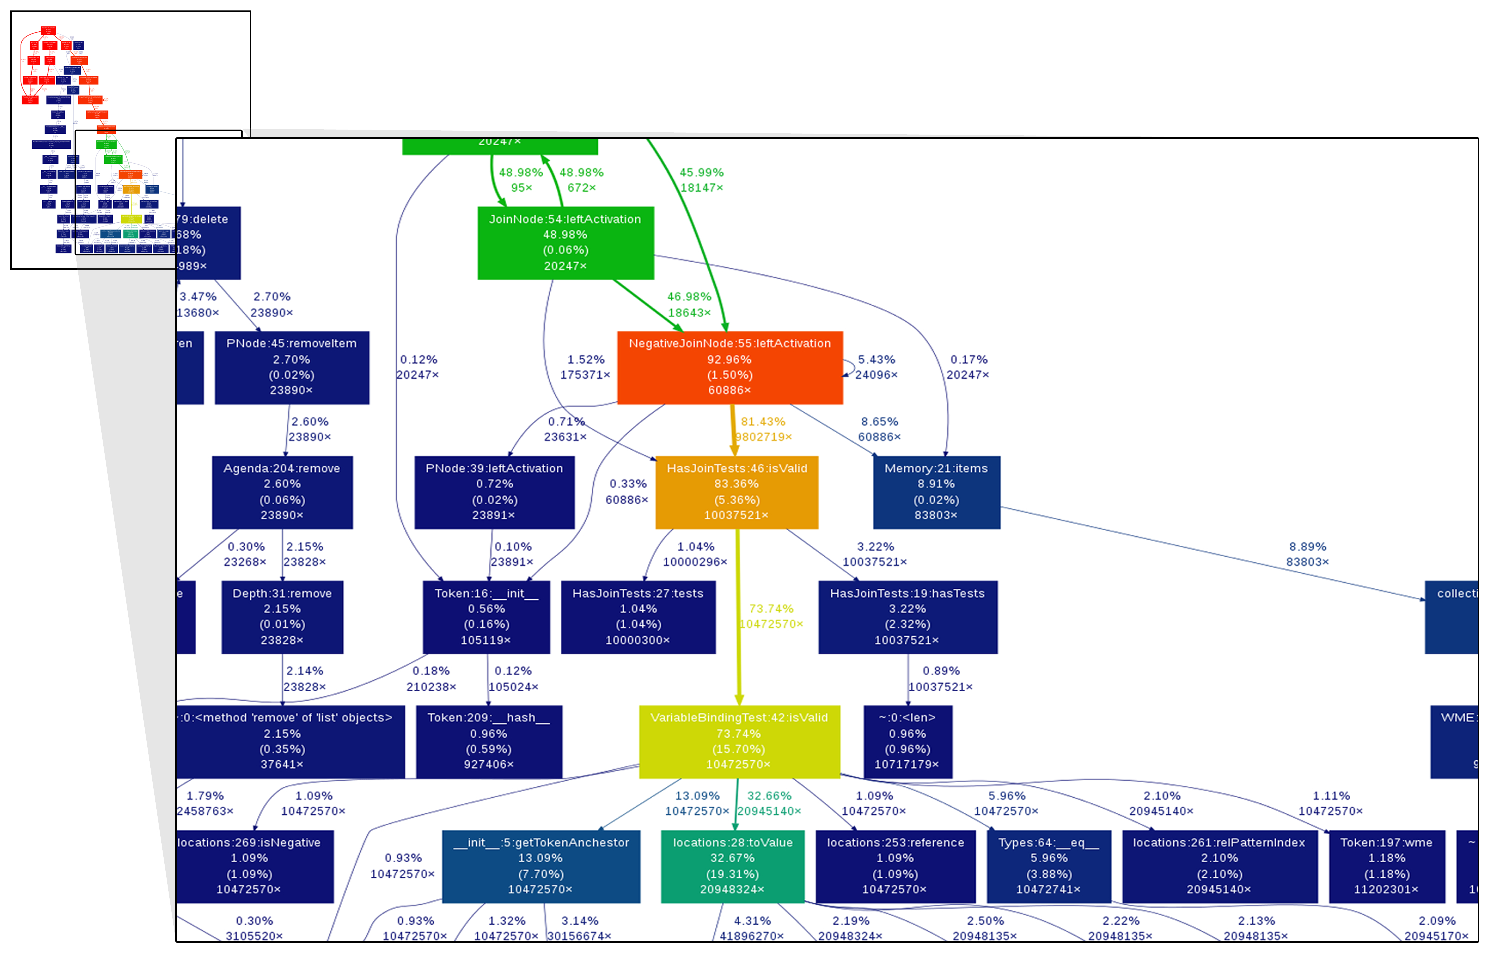
\includegraphics[width=1.3\textwidth, angle=270, viewport=0 0 718 456]{Immagini/Capitolo3/Profile-sudoku.pdf}
\caption[Profilazione dell'esecuzione del benchmark \emph{Sudoku}]{Profilazione dell'esecuzione del benchmark \emph{Sudoku}: grafico delle chiamate, dettaglio su \emph{VariableBindingTest}}\label{fig:profile-sudoku}
\end{figure}


Il benchmark \emph{Sudoku}, nell'implementazione distribuita insieme al software CLIPS~\cite{clipssudoku}, consente di valutare le prestazioni dei sistemi stressando i nodi della \emph{Beta-Network} generando una grande attività nei nodi Join positivi e negativi (\figurename~\ref{fig:profile-sudoku}). Le regole utilizzate per la formalizzazione delle strategie utilizzano condizioni simili, garantendo un'alta percentuale di condivisione dei nodi \emph{alpha}~\cite{rbsbench}. I test sono stati eseguiti utilizzando griglie di dimensioni $9 \times 9$ ($n = 3$) e due dataset differenti\footnote{grid3x3-p13: http://clipsrules.svn.sourceforge.net/viewvc/clipsrules/examples/sudoku/ puzzles/grid3x3-p13.clp?revision=93}$^,$\footnote{grid3x3-p15: http://clipsrules.svn.sourceforge.net/viewvc/clipsrules/examples/sudoku/ puzzles/grid3x3-p15.clp?revision=93}.

Di seguito (\tablename~\ref{tab:bench-sudoku}) sono proposti i risultati dei test effettuati sui sistemi CLIPS, MyCLIPS (localmente, tramite Terminale) e MyCLIPS (in remoto, tramite una RemoteShell).


\begin{table}[h]
\caption{Tempi d'esecuzione del benchmark \emph{Sudoku} per i dataset \emph{grid3x3-p13} e \emph{grid3x3-p15}}\label{tab:bench-sudoku}
\centering
\begin{tabular}{|c||c|c|}
\hline 
\multicolumn{3}{|c|}{Sudoku} \\ 
\hline 
 & \multicolumn{2}{c|}{Puzzle} \\ 
\hline 
Sistema & grid3x3-p13 & grid3x3-p15 \\ 
\hline\hline
CLIPS (6.24) & 5.315 & 8.488 \\ 
\hline 
MyCLIPS (locale) & 712.4 & 981.2 \\ 
\hline 
MyCLIPS (server) & 705.8 & 974.8 \\ 
\hline 
\end{tabular} 
\end{table}


\subsubsection{Monkey}

Il benchmark \emph{Monkey} fa riferimento ad un problema classico di pianificazione: l'obiettivo del problema è individuare la sequenza di azioni che consentono ad una scimmia di mangiare un casco di banane nascosto all'interno di un forziere chiuso a chiave posto in cima ad una pila di oggetti. La chiave che consente l'apertura del forziere è nascosta all'interno di un secondo forziere, anch'esso posto su una pila di oggetti. La scimmia è in grado di spostarsi nell'ambiente prendere, scaraventare e trasportare oggetti, oltre che utilizzare le chiavi per aprire i forzieri. 

L'implementazione utilizzata per la risoluzione è quella distribuita insieme al software CLIPS~\cite{clipsmab}: durante la risoluzione del problema vengono visualizzate sullo schermo le operazioni svolte dalla scimmia\footnote{La soluzione consiste di 42 operazioni consecutive}.

Di seguito (\tablename~\ref{tab:bench-monkey}) sono proposti i risultati dei test effettuati sui sistemi CLIPS, MyCLIPS (localmente, tramite Terminale) e MyCLIPS (in remoto, tramite una RemoteShell).


\begin{table}[h]
\caption{Tempi d'esecuzione del benchmark \emph{Monkey}}\label{tab:bench-monkey}
\centering
\begin{tabular}{|c||c|}
\hline 
\multicolumn{2}{c|}{Monkey} \\ 
\hline 
Sistema & Tempo \\ 
\hline\hline
CLIPS (6.24) & 0.004 \\ 
\hline 
MyCLIPS (locale) & 0.111 \\ 
\hline 
MyCLIPS (server) & 0.779 \\ 
\hline 
\end{tabular} 
\end{table}

\subsection{Osservazioni}

Grazie ai vari test effettuati è possibile affermare che le capacità del sistema prodotto risultano paragonabili a quelle del software di riferimento CLIPS. 
%La capacità di utilizzare artefatti e sistemi originariamente realizzati per il sistema di riferimento senza la necessità di apportare modifiche (escludendo le estensioni del sottosistema COOL), dimostra la possibilità di sostituire il primo sistema in maniera trasparente. 
I test hanno mostrato un livello di compatibilità di sistema che va al di là della sola portabilità degli artefatti: la sequenza delle attivazioni ed i relativi processi di ragionamento simulati dai sistemi risultano costanti in entrambi gli \emph{environment}. Sia i risultati che le modalità con le quali sono stati ottenuti vengono replicati esattamente dal prototipo realizzato.

Sebbene il divario in termini prestazionali sia evidente, l'obiettivo di questo elaborato era quello di realizzare un \emph{environment} funzionate con finalità didattiche e di ricerca, una base per sviluppi futuri. La scelta stessa del linguaggio è stata effettuata trascurando le problematiche di tipo prestazionale e privilegiando invece criteri di selezione come la facilità e rapidità di sviluppo e le possibilità di estensione offerte. Come emerso da diverse comparazioni effettuate fra linguaggi~\cite{prashant2008}~\cite{prechelt2000}~\cite{naiditch1999}, la valutazione della prestazione pura espressa in termini di tempo non vede Python emergere fra i migliori~\cite{cpybench}~\cite{prashant2008}~\cite{prechelt2000}. Il divario misurato tramite l'utilizzo della \emph{benchmark suite} in~\cite{cpybench} vede il linguaggio C risultare fino a cento volte più rapido rispetto a Python (\figurename~\ref{fig:c-vs-python-bench}). Chiaramente si propongono questi dati consci del fatto che trarre conclusioni semplicemente basandosi su numeri e senza effettuare i dovuti \emph{distinguo} non rappresenta un approccio efficace ad un problema tanto complesso quanto lo è la valutazione empirica delle prestazioni di un linguaggio di programmazione~\cite{algorithms}. 

Le ridotte prestazioni offerte dal linguaggio, non sono state ritenute una ragione sufficiente ad invalidare la preferenza espressa, soprattutto tenendo conto dei vantaggi che la soluzione ha offerto durante lo sviluppo del prototipo e che può potenzialmente offrire durante l'ulteriore sviluppo del sistema, principale obiettivo di questa tesi. Il \emph{Vincolo-7} non poneva delle limitazioni di rapidità alla soluzione prodotta se non quella di rendere possibile un confronto fra il prototipo e CLIPS utilizzando strumenti già fruttati in passato per questa finalità~\cite{rbsbench}~\cite{ops5bench}~\cite{brantetal91}.


\begin{figure}
\centering
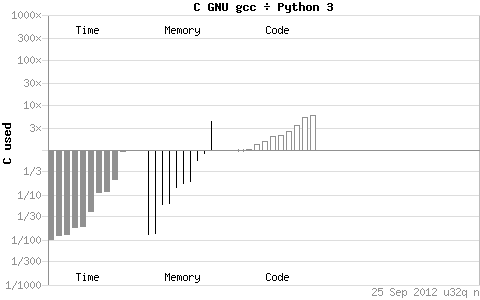
\includegraphics[width=0.8\textwidth]{Immagini/Capitolo3/c-vs-python.png}
\caption{Python 3 vs C: esecuzione della \emph{benchmark suite}~\cite{cpybench}  }\label{fig:c-vs-python-bench}
\end{figure}

Analizzando i risultati in ambito locale, si può evidenziare come il prototipo risulti fra le 20 e le 130 volte più lento rispetto al software di riferimento. I risultati migliori sono stati ottenuti nel benchmark \emph{Monkey}, dove la relativa semplicità del test ha permesso di marcare risultati ben al di sotto della soglia attesa. Le differenze risultano lievemente al di sotto delle attese anche per i test \emph{Manners} con 8 e 16 ospiti. Il divario si fa più marcato nel momento in cui la dimensione del dataset e la complessità dei test cresce, evidenziando maggiormente i limiti della soluzione proposta.

Quello che invece risulta più interessante è l'analisi dell'andamento del \emph{gap} prestazionale evidenziato dai test differenti (\figurename~\ref{fig:myclips-vs-clips-bench}). Il rapporto fra il prototipo e il software di riferimento è rimasto pressoché costante (compreso fra le 100 e 130 volte) anche a fronte di un aumento dei tempi reali di esecuzione dell'ordine di 40 volte, dimostrando una corrispondenza di comportamento fra il software di riferimento ed il sistema proposto in rapporto all'aumento della complessità dei test.


\begin{figure}
\begin{minipage}[b]{6.5cm}
	\centering
	\resizebox{6cm}{!}{
	\begin{tikzpicture}
	\begin{axis}[ylabel={MyCLIPS usa (tempo)},
				ybar,
				ymin=20,
				ymax=200,
				xtick=data,
				ymajorgrids=true,
				%xtick pos=left,
				x tick label style=%
					{rotate=45,	anchor=east	},
				%xticklabel interval boundaries,
				symbolic x coords={
					$manners-8$,
					$manners-16$,
					$manners-32$,
					$manners-64$,
					$sudoku-p13$,
					$sudoku-p15$,
					$monkey$},
				title style={align=center},
				title={MyCLIPS (locale) $\div$ CLIPS}]
	\addplot [%ybar interval,
				fill=grigio-chiarissimo,
				draw=black] coordinates
	{($manners-8$, 62.2) 
	($manners-16$, 59.3)
	($manners-32$, 112.8)
	($manners-64$, 113.4)
	($sudoku-p13$, 134) 
	($sudoku-p15$, 115.5)
	($monkey$, 27.7)
	};
	\end{axis}
	\end{tikzpicture}
	}
\end{minipage}
\ \hspace{2mm} \hspace{3mm} \
\begin{minipage}[b]{6.5cm}
	\centering
	\resizebox{6cm}{!}{
	\begin{tikzpicture}
	\begin{axis}[ylabel={MyCLIPS usa (tempo)},
				ybar,
				ymin=20,
				ymax=200,
				xtick=data,
				ymajorgrids=true,
				%xtick pos=left,
				x tick label style=%
					{rotate=45,	anchor=east	},
				%xticklabel interval boundaries,
				symbolic x coords={
					$manners-8$,
					$manners-16$,
					$manners-32$,
					$manners-64$,
					$sudoku-p13$,
					$sudoku-p15$,
					$monkey$},
				title style={align=center},
				title={MyCLIPS (server) $\div$ CLIPS}]
	\addplot [%ybar interval,
				fill=grigio-chiarissimo,
				draw=black] coordinates
	{($manners-8$, 65.4) 
	($manners-16$, 61.3)
	($manners-32$, 118.9)
	($manners-64$, 118)
	($sudoku-p13$, 132.7) 
	($sudoku-p15$, 114.8)
	($monkey$, 194)
	};
	\end{axis}
	\end{tikzpicture}
	}
\end{minipage}
\caption[Grafici dei rapporti prestazionali fra MyCLIPS e CLIPS]{Grafici dei rapporti prestazionali fra MyCLIPS e CLIPS: a sinistra il confronto con un'istanza locale di MyCLIPS, a destra con una server}\label{fig:myclips-vs-clips-bench}
\end{figure}

L'analisi dei risultati ottenuti utilizzando il sistema tramite un'istanza server evidenzia una corrispondenza con i risultati ottenuti tramite utilizzo locale. L'unica eccezione risiede nei risultati del benchmark \emph{Monkey}, dove si riscontra un peggioramento delle prestazioni evidente. Bisogna però effettuare delle valutazioni particolari per comprendere appieno il risultato del singolo test: il benchmark esegue durante il processo 42 operazioni di \emph{output} a fronte di un tempo di esecuzione di un decimo di secondo. In questo caso, i tempi richiesti per le operazioni di inoltro dei dati verso lo \emph{stream} remoto dominano quelli di esecuzione del test in sé. Lo stesso fenomeno non si presenta durante l'esecuzione del benchmark \emph{Sudoku}: sebbene, in termini assoluti, il test esegua un maggior numero di operazioni di output su \emph{stream} (oltre 200), i risultati non risultano influenzati data la maggior durata dello stesso. Si conclude quindi che l'utilizzo remoto del prototipo offra prestazioni e possibilità in linea con un utilizzo locale.

%\section{Conclusioni}

%L'integrazione degli strumenti di sviluppo per sistemi esperti con tecnologie orientate alla distribuzione degli stessi in ambito \emph{web} ha offerto lo spunto per questo lavoro di tesi. Prendendo come riferimento le funzionalità offerte da un \emph{environment} di grande adozione come CLIPS, è stata progettata e quindi realizzata una soluzione compatibile che enfatizzasse le capacità di estensibilità e integrazione offerte dal linguaggio di programmazione scelto per la realizzazione del prototipo: Python. Al fine di saggiare la flessibilità della soluzione proposta è stata eseguita l'integrazione della soluzione in un modello d'architettura \emph{client-server} e quindi valutato l'impatto che l'adozione di questa tecnologia ha avuto sulle prestazioni complessive del sistema.

%Durante questa trattazione è stata fornita una definizione di sistemi esperti, approfondendo le tematiche relative al loro processo di sviluppo e all'ambito di utilizzo degli stessi. L'attenzione è stata quindi focalizzata verso le tecniche utilizzate per la formalizzazione della conoscenza in strutture adeguate alla computazione e quindi offerta una classificazione generale degli strumenti di sviluppo per sistemi esperti.
%Nella seconda e terza parte sono state approfondite le problematiche relative alla progettazione e alla realizzazione di un prototipo funzionante di \emph{environment} multi-paradigmatico, successivamente sottoposto ad una valutazione per testarne la correttezza e le prestazioni.

%Da quanto osservato durante la sperimentazione si può affermare che i risultati ottenuti sono in linea con le attese. Il livello di compatibilità con il sistema di riferimento risulta soddisfacente, i costrutti più utilizzati e considerati indispensabili vengono resi disponibili dal prototipo e i comportamenti riscontrati risultano trovano corrispondenza fra i due sistemi. L'analisi della prestazione ha mostrato un \emph{gap} abbastanza evidente, ma il degrado delle prestazioni, superato un valore di soglia, replica esattamente il comportamento riscontrato nella soluzione di riferimento. Una delle cause alla base delle minori prestazioni è il linguaggio utilizzato per l'implementazione del prototipo, ma non è l'unica. L'analisi del grafico delle chiamate (\figurename~\ref{fig:profile-sudoku}) generato durante la profilazione del benchmark \emph{Sudoku} ha messo in luce due criticità, sicuramente concause delle scarse prestazioni ottenute nello specifico test:
%\begin{enumerate}
%	\item la realizzazione scelta per la rappresentazione dei Token nel sistema utilizza una struttura ad albero per ridurre il consumo di memoria e permettere una condivisione delle informazioni~\cite{Doorenbos95productionmatching}. Questo approccio ha comportato un maggior dispendio di tempo per l'esecuzione delle procedure di \emph{matching} a causa della forma utilizzata per serializzazione delle regole nello specifico test.
	
%	\item l'implementazione dei pattern \emph{Test-CE} prevede l'esecuzione di chiamate a funzione senza prevedere alcun sistema di \emph{caching} dei risultati. Verifiche successive richiedono una nuova esecuzione della funzione anche nei casi in cui gli input siano identici a quelli di valutazioni precedenti.
%\end{enumerate}



%Il risultato di questo lavoro è un sistema che può rappresentare una buona base di partenza per ulteriori evoluzioni del sistema. 
%Le capacità realizzate rappresentano una porzione delle funzionalità che vengono richieste ad un \emph{environment per sistemi esperti} della corrente generazione. Le scelte effettuate durante la progettazione e la realizzazione del sistema hanno avuto come priorità quella di rendere il sistema modificabile, analizzabile ed estendibile con facilità. Lo sviluppo della componente server è stato un modo per saggiarne la flessibilità trasferendo il normale modello di interazione anche attraverso un'architettura tanto differente quanto quella \emph{client-server}.


%\subsection{Sviluppi futuri}

%L'approfondimento di alcune delle mancanze del prototipo o l'aggiunta di ulteriori funzionalità potrebbe offrire lo spunto per ulteriori evoluzioni del sistema e nuovi ambiti di ricerca:
%\begin{itemize}
%	\item l'integrazione di un \emph{regime di controllo} alternativo basato sul \emph{backward-chaining} o su approcci ibridi, garantendo agli ingegneri della conoscenza maggiore flessibilità durante le fasi di progettazione.
	
%	\item l'integrazione del paradigma di programmazione basato su oggetti nel linguaggio di specifica.
	
%	\item la valutazione delle prestazioni offerte dal sistema utilizzando algoritmi di matching differenti come ad esempio TREAT~\cite{Miranker:1987:TBM:899610}~\cite{Miranker:1987:TBM:1856670.1856678} o LEAPS~\cite{Batory:1994:LA:899216}.	
	
%	\item approfondimento delle problematiche relative alle prestazioni generali del sistema, eseguendo una nuova valutazione sulle tecnologie impiegate per la realizzazione dell'artefatto.
	
%	\item l'integrazione di funzionalità che agevolino lo svolgimento di attività comuni  dei sistemi esperti come la spiegazione dell'inferenza.
	
%	\item la fusione nel motore inferenziale di strumenti per la gestione dell'incertezza e della logica \emph{Fuzzy}.
%\end{itemize}
